%\documentclass[spanish,a4paper,11pt,oneside,links]{report}
\documentclass[spanish,a4paper,oneside,12pt,openright]{book}

\usepackage{mathptmx}
\usepackage{graphicx}
\usepackage{amsmath,amsfonts,amssymb}
\usepackage[utf8]{inputenc}
\usepackage[spanish, es-tabla]{babel}
\usepackage[Algoritmo]{algorithm}
\usepackage{algpseudocode}
\usepackage{url}
\usepackage{fancyhdr}
\usepackage{epstopdf}
\usepackage{minted}
\usepackage{csquotes}
\usepackage{rotating}
\usepackage{etoolbox}
\usepackage{zref-xr}
\usepackage{hyperref}
%\usepackage[authoryear,round,longnamesfirst]{natbib}
\usepackage[numbers,square]{natbib}
\setcitestyle{comma}
\usepackage{multicol}
\usepackage{spverbatim}
\usepackage[pdf]{graphviz}
\usepackage{dirtree}
\usepackage{tabularx}
    \newcolumntype{L}{>{\raggedright\arraybackslash}X}
\usepackage{emptypage}
\usepackage[acronym,shortcuts]{glossaries}
\usepackage{markdown}
\usepackage{booktabs}
\usepackage{multirow}
\usepackage{xcolor}
\usepackage{changepage}
\usepackage{tcolorbox}
\usepackage{listings}
\usepackage{datetime}
\usepackage{subcaption}
\usepackage{tikz} \usetikzlibrary{arrows.meta,positioning,decorations.pathreplacing}
\usepackage{float}
\usepackage{array}
\usepackage{setspace}
\usepackage{pdfpages}

% Rutas de figuras e inputs relativas a Latex/ (un nivel arriba)
\graphicspath{{../}}

\newcommand{\capitalmonthname}[1]{%
  \ifcase#1\or
    Enero\or Febrero\or Marzo\or Abril\or Mayo\or Junio\or
    Julio\or Agosto\or Septiembre\or Octubre\or Noviembre\or Diciembre
  \fi
}

\newdateformat{monthyeardate}{%
  \capitalmonthname{\THEMONTH}, \THEYEAR}

\newcommand{\tfcTitle}{Estimación de la edad cerebral mediante autoencoders variacionales y aprendizaje multimodal a partir de conectividad funcional, datos estructurales y variables sociodemográficas}
\newcommand{\tfcAuthor}{Nicolás Marcelo Bazán}
\newcommand{\authorname}{\tfcAuthor}
\newcommand{\tfcAdvisors}{Damián Barsotti \\ Gabriel Della Bella}
\newcommand{\tfcGrade}{Licenciado en Ciencias de la Computación}
\newcommand{\tfcFaculty}{Facultad De Matemática, Astronomía, Física Y Computación}
\newcommand{\tfcCollege}{Universidad Nacional de Córdoba}
\newcommand{\tfcDefenseDate}{Mayo, 2026}

\setlength{\headheight}{25.07225pt}
\addtolength{\topmargin}{-12.0pt}

% wide page for side by side figures, tables, etc
\newlength{\offsetpage}
\setlength{\offsetpage}{1.0cm}
\newenvironment{widepage}{\begin{adjustwidth}{-\offsetpage}{-\offsetpage}%
    \addtolength{\textwidth}{2\offsetpage}}%
{\end{adjustwidth}}

\newtheorem{definition}{Definición}

\renewcommand{\listalgorithmname}{Índice de Algoritmos}

\addto\extrasspanish{
    \renewcommand{\sectionautorefname}{Sec.}
}


\DeclareMathOperator*{\argmax}{arg\,max}  % in your preamble
\DeclareMathOperator*{\argmin}{arg\,min}  % in your preamble

\DeclareMathOperator*{\minimize}{minimize}
\DeclareMathOperator*{\maximize}{maximize}

\makeglossaries

% Acrónimos y glosario (glossaries)

% Neuroimagen
\newacronym{mri}{MRI}{Magnetic Resonance Imaging}
\newacronym{fmri}{fMRI}{functional Magnetic Resonance Imaging}
\newacronym{bold}{BOLD}{Blood-Oxygenation-Level Dependent}
\newacronym{fc}{FC}{Functional Connectivity}
\newacronym{aal}{AAL}{Automated Anatomical Labeling}
\newacronym{vbm}{VBM}{Voxel-Based Morphometry}
\newacronym{roi}{ROI}{Region of Interest}

% Diagnósticos clínicos
\newacronym{cn}{CN}{Cognitively Normal}
\newacronym{ad}{AD}{Alzheimer's Disease}
\newacronym{ftd}{FTD}{Frontotemporal Dementia}

% Modelos y métodos
\newacronym{vae}{VAE}{Variational Autoencoder}
\newacronym{pca}{PCA}{Principal Component Analysis}
\newacronym{xgboost}{XGBoost}{eXtreme Gradient Boosting}
\newacronym{svr}{SVR}{Support Vector Regression}
\newacronym{kl}{KL}{Kullback--Leibler}
\newacronym{elbo}{ELBO}{Evidence Lower Bound}
\newacronym{tpe}{TPE}{Tree-structured Parzen Estimator}
\newacronym{hpo}{HPO}{Hyperparameter Optimization}
\newacronym{gnn}{GNN}{Graph Neural Network}
\newacronym{cnn}{CNN}{Convolutional Neural Network}
\newacronym{cv}{CV}{Cross-Validation}
\newacronym{rbf}{RBF}{Radial Basis Function}

% Estadística
\newacronym{anova}{ANOVA}{Analysis of Variance}

% Métricas
\newacronym{mae}{MAE}{Mean Absolute Error}
\newacronym{rmse}{RMSE}{Root Mean Squared Error}
\newacronym{mse}{MSE}{Mean Squared Error}
\newacronym{sse}{SSE}{Sum of Squared Errors}

\lhead[]{\rightmark}
\chead[]{}
\rhead[\leftmark]{}
\renewcommand{\headrulewidth}{0.5pt}

\fancypagestyle{plain}{
\fancyhead[L]{}
\fancyhead[C]{}
\fancyhead[R]{}
\renewcommand{\headrulewidth}{0pt}
}

\pagestyle{fancy}

\widowpenalty 10000
\clubpenalty 10000

% Editorial/review commands (highlighting and placeholders)
% Review commands removed for final version

\renewcommand{\listingscaption}{Algoritmo}
\renewcommand{\listoflistingscaption}{Lista de algoritmos}

%\usemintedstyle{algol_nu}
%https://pygments.org/styles/

\setminted{
    breaklines=true
}

\renewcommand{\listingscaption}{Código}
\renewcommand{\thelisting}{\thesection.\arabic{listing}}
\preto\section{\setcounter{listing}{0}}

\begin{document}



% % Caratula
\begin{titlepage}

% LOGOS SUPERIORES
\noindent
\begin{minipage}[t]{0.5\linewidth}
    \flushleft
    
\includegraphics[width=6cm]{00_tapa/figures/logo_unc.png} % Descomentar si tienes la imagen
\end{minipage}%
\begin{minipage}[t]{0.5\linewidth}
    \flushright
    
\includegraphics[width=6cm]{00_tapa/figures/logo_famaf.png} % Descomentar si tienes la imagen
\end{minipage}

\vspace{1.2cm} % Espacio vertical para separar

% TÍTULO Y AUTOR
\begin{center}
    \begin{spacing}{1.5}
    {\LARGE \textbf{\tfcTitle}}
    \end{spacing}
    \vspace{0.8cm}
    {\large por}\\[0.4cm]
    {\Large \textbf{\tfcAuthor}}
\end{center}

\vspace{0.6cm}

% TEXTO DESCRIPTIVO
\noindent
Presentado ante la \textbf{\MakeUppercase{\tfcFaculty}} como parte de los requerimientos para la obtención del grado de \tfcGrade{} de la

\begin{center}
    \textbf{\MakeUppercase{\tfcCollege}}
\end{center}

\vspace{0.4cm}

\noindent
\begin{center}
    \tfcDefenseDate
\end{center}

\vspace{0.2cm}

% DIRECTOR/A
\noindent
\begin{center}
Directores: \\ \tfcAdvisors
\end{center}

\vfill % Espacio hasta el final de la página

% LICENCIA CREATIVE COMMONS
\begin{center}
    
\includegraphics[width=3cm]{00_tapa/figures/by-nc-sa.png}\\[0.1cm]
    Este trabajo se distribuye bajo una licencia\\
    \href{https://creativecommons.org/licenses/by-nc-sa/4.0/?ref=chooser-v1}{Creative Commons Atribución-NoComercial-CompartirIgual 4.0 Internacional}
\end{center}

\vspace{0.3cm}

\end{titlepage}
 \cleardoublepage


\pagenumbering{gobble}
Certifico que el trabajo incluido en este documento es el resultado de tareas de investigación
originales y que no ha sido presentado para optar a un título en ninguna otra
Universidad o Institución.

\vspace{3cm}
\begin{flushright}
\authorname
\end{flushright}
\cleardoublepage

% Agradecimientos

%\chapter*{Reconocimientos}
%\pagenumbering{Roman} % para comenzar la numeracion de paginas en numeros romanos
%\addcontentsline{toc}{chapter}{Reconocimientos} % si queremos que aparezca en el índice
%\markboth{RECONOCIMIENTOS}{RECONOCIMIENTOS} % encabezado
%Esta Tesis fue desarrollada gracias a la ayuda económica de ...


%\phantom{p. 1}
\clearpage
\thispagestyle{empty}
\phantom{p. 2}
\clearpage

\chapter*{Agradecimientos} % si no queremos que añada la palabra "Capitulo"
\pagenumbering{Roman} % para comenzar la numeracion de paginas en numeros romanos
\addcontentsline{toc}{chapter}{Agradecimientos} % si queremos que aparezca en el índice
\markboth{AGRADECIMIENTOS}{AGRADECIMIENTOS} % encabezado
Quisiera agradecer a la Universidad Nacional de Córdoba y a la Facultad de Matemática, Astronomía, Física y Computación por haberme dado la posibilidad de acceder a una educación libre, gratuita y de calidad, y por permitirme realizar este trabajo final de grado que culmina una etapa importante en mi vida y da comienzo a otra.

A mis directores, Damián Barsotti, Gabriel Della Bella y Pablo Barttfeld, por su guía, su paciencia y su compromiso en todo momento.

A cada compañero y profesor con quienes tuve la oportunidad de compartir estos años de estudio, por la compañía y por todo el conocimiento y las enseñanzas que me brindaron.

A mis compañeros de trabajo en Ualabee por permitirme desarrollarme profesionalmente, por las oportunidades que me brindaron y por darme el espacio para enfocarme en mis estudios cuando lo necesitaba.

A mis amigos de la facultad, por haberme enseñado tanto en lo académico como en lo personal, por las anécdotas, las horas de estudio y por hacer de la vida universitaria algo más divertido.
A mis amigos fuera de la facultad, que también me acompañaron y estuvieron dispuestos a escucharme y ayudarme cuando lo necesitaba.

Por último y más importante, a mi familia quienes son mi sostén y apoyo incondicional.

A mi papá Marcelo y a mi mamá Judith, quienes se esforzaron por darme la mejor educación posible y me brindaron todo para que no me faltara nada, incluso en los momentos más difíciles.
A mis hermanos, Matías y Carolina, que se han preocupado por mí, aconsejado y acompañado en todo momento.
A mis sobrinos, Felipe y Alma, que siempre me sacan una sonrisa y traen alegría a la familia.
A mis tíos y tías, abuelos y abuelas; en particular a mis tías Marta y Silvia, que se han preocupado por mi educación y mi salud en todo momento.
A todos ellos, a los que están y a los que ya no están con nosotros pero siguen presentes en el recuerdo, por creer en mí incluso cuando yo no lo hacía y por darme la fuerza para seguir adelante.

Y por último, a mí mismo. Por todo el esfuerzo, el sacrificio, la paciencia y la dedicación que puse en estos años de carrera y formación, a pesar de las dificultades que se presentaron en el camino. Por haber aprendido a enfrentarlas y superarlas.


% Resumen / Abstract

\phantom{p. 1}
\clearpage
\thispagestyle{empty}
\phantom{p. 2}
\clearpage

\chapter*{Resumen} % si no queremos que añada la palabra "Capitulo"
\addcontentsline{toc}{chapter}{Resumen} % si queremos que aparezca en el índice
\markboth{RESUMEN}{RESUMEN} % encabezado
La estimación de la edad cerebral a partir de datos de neuroimagen permite cuantificar el envejecimiento del cerebro y detectar desviaciones asociadas a enfermedades neurodegenerativas. La diferencia entre la edad predicha y la edad cronológica ---la \textit{brain age gap}--- constituye un potencial biomarcador de envejecimiento acelerado.

En este trabajo se propone un pipeline multimodal que integra conectividad funcional derivada de fMRI en reposo, comprimida mediante un $\beta$-VAE, con medidas volumétricas de materia gris (T1w) para predecir la edad cerebral con XGBoost. El pipeline fue evaluado sobre $N = 1\,245$ sujetos de la cohorte multicéntrica latinoamericana RedLaT, alcanzando un error absoluto medio (MAE) de 5,62 años. La integración de ambas modalidades superó el uso de cualquiera por separado, y la reducción de dimensionalidad resultó más determinante que la elección entre métodos lineales y no lineales o entre familias de regresores.

Se analizó además el impacto de variables demográficas ---años de educación y sitio de adquisición--- sobre la predicción y la brain age gap. La inclusión de estas variables como features adicionales redujo el MAE a 5,17 años, mientras que el sitio de adquisición emergió como el principal confundidor entre centros. La evaluación del pipeline como biomarcador mediante entrenamiento exclusivo en controles sanos mostró señales prometedoras al incorporar información demográfica, aunque el tamaño de la muestra disponible limitó su aplicabilidad clínica. El pipeline es modular y reutilizable, lo que facilita su adaptación a cohortes más amplias y la incorporación de nuevas variables.

\vspace{1em}
\noindent\textbf{Palabras clave:} edad cerebral, neuroimagen, conectividad funcional, fMRI, autoencoder variacional, XGBoost, datos multimodales, brain age gap, variables demográficas, cohorte latinoamericana.


\phantom{p. 1}
\clearpage
\thispagestyle{empty}

\chapter*{Abstract} % si no queremos que añada la palabra "Capitulo"
\addcontentsline{toc}{chapter}{Abstract} % si queremos que aparezca en el índice
\markboth{ABSTRACT}{ABSTRACT} % encabezado
Brain age estimation from neuroimaging data enables the quantification of brain aging and the detection of deviations associated with neurodegenerative diseases. The difference between predicted and chronological age ---the brain age gap--- constitutes a potential biomarker of accelerated aging.

This work proposes a multimodal pipeline that integrates resting-state fMRI functional connectivity, compressed via a $\beta$-VAE (beta-variational autoencoder), with T1-weighted gray matter volumes to predict brain age using XGBoost. The pipeline was evaluated on $N = 1{,}245$ subjects from the multicentric Latin American cohort RedLaT, achieving a mean absolute error (MAE) of 5.62 years. Integrating both modalities outperformed using either one alone, and dimensionality reduction proved more important than the choice between linear and nonlinear methods or among regressor families.

The impact of demographic variables ---years of education and acquisition site--- on prediction and the brain age gap was also analyzed. Including these variables as additional features reduced the MAE to 5.17 years, while the acquisition site emerged as the main confounder across centers. Evaluation of the pipeline as a biomarker through training exclusively on cognitively normal subjects showed promising signals when incorporating demographic information, although the available sample size limited clinical applicability. The pipeline is modular and reusable, facilitating its adaptation to larger cohorts and the incorporation of new variables.

\vspace{1em}
\noindent\textbf{Keywords:} brain age, neuroimaging, functional connectivity, fMRI, variational autoencoder, XGBoost, multimodal data, brain age gap, demographic variables, Latin American cohort.


\clearpage
\phantom{p. 1}
\thispagestyle{empty}



% Glosario

\renewcommand*\glspostdescription{\dotfill}
\setlength{\glslistdottedwidth}{1\textwidth}
\setlength{\glsdescwidth}{0.89\textwidth}
\markboth{Glosario}{Glosario} % encabezado
\glsaddall
\printglossary[type=\acronymtype,title=Glosario]
\addcontentsline{toc}{chapter}{Glosario}


% Índice de contenidos
\phantom{p. 1}
\clearpage

\tableofcontents % indice de contenidos

\phantom{p. 1}
\clearpage
\thispagestyle{empty}
\phantom{p. 2}
\clearpage

% Contenido (capítulos)

\pagenumbering{arabic}
\setcounter{page}{1}

% Cap 1: Introducción
\chapter{Introducción}
\label{chapter:intro}

El cerebro humano experimenta cambios constantes a lo largo de la vida como parte del proceso normal de envejecimiento. Algunos de estos cambios son progresivos, como la mielinización (crucial para el desarrollo cognitivo) o el desarrollo celular, mientras que otros reflejan procesos regresivos, entre ellos la pérdida neuronal, la reducción del volumen de materia gris y el adelgazamiento cortical \cite{good2001voxel, fjell2010structural, raz2005regional}. La combinación de estos fenómenos produce un patrón característico de envejecimiento cerebral que, en la mayoría de los casos, ocurre de manera gradual y predecible.

Sin embargo, distintas enfermedades neurodegenerativas y psiquiátricas pueden alterar este curso natural. En patologías como la enfermedad de Alzheimer, por ejemplo, se observa una aceleración de la atrofia cerebral, lo que provoca que el cerebro de un paciente “aparente” una edad mayor a su edad cronológica \cite{franke2010estimating}. Este tipo de observaciones motivó el desarrollo del concepto de edad cerebral (brain age), entendido como una estimación de la edad biológica del cerebro a partir de datos de neuroimagen, generalmente obtenida mediante modelos predictivos entrenados sobre poblaciones sanas. A partir de esta estimación es posible calcular la brecha de edad cerebral (brain age gap), definida como la diferencia entre la edad predicha y la edad real del individuo \cite{smith2019estimation}. Una brecha positiva puede interpretarse como un envejecimiento acelerado, mientras que una brecha negativa sugiere resiliencia o envejecimiento más lento de lo esperado.


La estimación de la edad cerebral suele realizarse utilizando imágenes obtenidas mediante resonancia magnética (MRI). Las imágenes T1-weighted (T1w) permiten extraer información estructural del cerebro, como volúmenes de materia gris, materia blanca y líquido cefalorraquídeo \cite{franke2010estimating}. Por otro lado, las imágenes fMRI en reposo (resting-state fMRI) capturan fluctuaciones espontáneas de la actividad cerebral, a partir de las cuales es posible calcular medidas de conectividad funcional entre distintas regiones \cite{damoiseaux2006consistent, craddock2012whole}. Dado que estructura y función aportan información complementaria sobre el envejecimiento, el uso combinado de ambas modalidades ha demostrado ser una estrategia prometedora para mejorar la precisión de los modelos de predicción \cite{erus2015imaging, groves2012benefits}.


En este trabajo se aborda el problema de predecir la edad cerebral utilizando un enfoque multimodal. Para ello, se emplean matrices de conectividad funcional derivadas de fMRI y datos estructurales obtenidos a partir de imágenes T1w, evaluados sobre la cohorte multicéntrica latinoamericana RedLaT. Se analiza además la contribución de variables demográficas ---incluyendo sexo, años de educación y sitio de adquisición--- tanto mediante estudios de ablaciones (que investiga el rendimiento de un modelo mediante la eliminación de determinados componentes) como a través de su relación con la brain age gap. El uso de una cohorte latinoamericana, con su marcada heterogeneidad socioeconómica y cultural, permite explorar cómo factores demográficos asociados a las condiciones de vida en la región modulan la predicción de edad cerebral, un aspecto poco estudiado en la literatura existente, que se ha basado predominantemente en cohortes europeas y norteamericanas. Desde una perspectiva computacional, este trabajo propone un pipeline modular que combina técnicas de aprendizaje no supervisado ($\beta$-VAE), cuya elección se fundamenta en los buenos resultados reportados por autoencoders variacionales en análisis de neuroimagen \cite{vieira2017using} y en estimación de edad cerebral \cite{dufumier2024multi}, y modelos de regresión (XGBoost) para integrar información estructural y funcional en la estimación de la edad cerebral. Adicionalmente, se evalúa la viabilidad del pipeline como biomarcador de envejecimiento acelerado mediante el entrenamiento exclusivo en controles sanos, discutiendo las limitaciones impuestas por el tamaño de la cohorte disponible.


\section{Objetivos}

\subsection{Objetivo general}

Desarrollar y evaluar un pipeline de estimación de edad cerebral basado en la integración multimodal de datos de neuroimagen funcional y estructural, utilizando técnicas de aprendizaje profundo no supervisado y modelos de regresión supervisada, y analizar el impacto de variables demográficas y la viabilidad del pipeline como biomarcador de envejecimiento cerebral sobre una cohorte multicéntrica latinoamericana.

\subsection{Objetivos específicos}

\begin{enumerate}
    \item Implementar un autoencoder variacional con ponderación $\beta$ ($\beta$-VAE) para la reducción de dimensionalidad no lineal de matrices de conectividad funcional derivadas de fMRI.
    \item Integrar las representaciones latentes funcionales con features volumétricas de materia gris (T1w) para la predicción supervisada de la edad mediante XGBoost.
    \item Optimizar los hiperparámetros del VAE utilizando la predicción de edad como objetivo downstream, en lugar del error de reconstrucción.
    \item Cuantificar la contribución de cada modalidad y variable mediante un estudio de ablaciones.
    \item Comparar el enfoque de reducción no lineal (VAE) con un baseline lineal (PCA) para evaluar la naturaleza de las relaciones en los datos de conectividad funcional.
    \item Evaluar el pipeline sobre una cohorte multicéntrica latinoamericana (RedLaT), incluyendo sujetos sanos y pacientes con enfermedades neurodegenerativas.
    \item Analizar el impacto de variables demográficas y socioeconómicas ---en particular los años de educación y el sitio de adquisición--- sobre la brain age gap y la predicción de edad cerebral en el contexto de una cohorte latinoamericana.
    \item Evaluar la viabilidad del pipeline como biomarcador de envejecimiento acelerado mediante el entrenamiento exclusivo en controles sanos, analizando la influencia del tamaño de la muestra sobre los resultados obtenidos.
\end{enumerate}


\section{Organización del trabajo}

Los capítulos de este trabajo se organizan de la siguiente manera:

En el Capítulo~\ref{chapter:marco_teorico} se presenta el marco teórico necesario para contextualizar el problema, abordando conceptos fundamentales de neuroimagen, aprendizaje automático, autoencoders variacionales y modelos basados en árboles. En el Capítulo~\ref{chapter:trabajo_relacionado} se revisan los trabajos previos en estimación de edad cerebral, incluyendo los métodos, datasets y resultados reportados en la literatura. En el Capítulo~\ref{chapter:datos_cohorte} se describen los datos utilizados, incluyendo las características de la cohorte RedLaT, las modalidades de neuroimagen disponibles y el proceso de integración de las fuentes de datos. El Capítulo~\ref{chapter:metodologia_pipeline} detalla la metodología propuesta y el pipeline implementado para la integración multimodal de la información y la estimación de la edad cerebral, incluyendo la arquitectura del $\beta$-VAE, el modelo de regresión XGBoost y la optimización de hiperparámetros con Optuna. En el Capítulo~\ref{chapter:resultados_discusion} se presentan los resultados obtenidos, el análisis de las métricas de desempeño, las ablaciones realizadas, la evaluación del entrenamiento exclusivo en controles sanos, el impacto de variables demográficas sobre la predicción y la brain age gap, y la discusión de los hallazgos en el contexto de la literatura existente. Finalmente, el Capítulo~\ref{chapter:conclu} resume las conclusiones del trabajo y plantea posibles líneas de investigación futura. \cleardoublepage

% Cap 2: Marco teórico
\chapter{Marco Teórico}
\label{chapter:marco_teorico}

% 2.1
\section{Bases neurobiológicas del envejecimiento cerebral}
\label{sec:bases_neuro}

Existe evidencia suficiente que demuestra que el cerebro experimenta cambios a lo largo de la vida como parte del proceso normal de envejecimiento. Estos cambios no implican necesariamente la presencia de una enfermedad, sino que forman parte de la evolución natural del cerebro con el paso del tiempo. Estudiar este proceso resulta de interés por múltiples razones, entre ellas la disminución progresiva de ciertas habilidades cognitivas y motrices, así como los cambios observados en la memoria y otras funciones mentales.

El envejecimiento cerebral se encuentra asociado a modificaciones inevitables en distintas propiedades del tejido cerebral. Entre los cambios más estudiados se encuentra la reducción del volumen de determinadas estructuras, así como alteraciones en la organización interna del cerebro. Estos procesos no afectan a todas las regiones de la misma manera ni con la misma intensidad, y su impacto puede variar considerablemente entre distintos individuos.

Estudios longitudinales en adultos sanos han mostrado que los cambios estructurales asociados al envejecimiento no se producen de manera uniforme en todo el cerebro. Si bien la reducción del volumen cerebral es un fenómeno ampliamente observado, su magnitud varía según la región analizada y entre distintos individuos. Estas diferencias indican que el envejecimiento cerebral no sigue un patrón único, sino que presenta trayectorias diversas tanto a nivel regional como individual, incluso en poblaciones sin diagnóstico de patologías neurodegenerativas \cite{raz2005regional}.

El análisis de los cambios cerebrales en personas sanas adquiere especial relevancia cuando se lo utiliza como referencia para comparar con procesos patológicos. Enfermedades neurodegenerativas como la enfermedad de Alzheimer (AD) o la demencia frontotemporal (FTD) presentan alteraciones estructurales que, en muchos casos, afectan regiones que también se ven modificadas durante el envejecimiento normal, aunque de forma más pronunciada. Esta superposición plantea interrogantes fundamentales acerca de cuán diferentes son los cambios producidos por una enfermedad neurodegenerativa respecto de aquellos propios del envejecimiento saludable.

Numerosos estudios han investigado la relación entre la edad y el volumen o grosor de diversas estructuras cerebrales, mostrando que algunas regiones presentan un deterioro más marcado mientras que otras se mantienen relativamente preservadas \cite{good2001voxel}. En este contexto, la materia gris resulta de particular interés, ya que desempeña un rol central en el procesamiento de la información y en el control de funciones como el pensamiento, la memoria y el movimiento. Evidencia previa indica que la cantidad de materia gris tiende a disminuir con la edad, y que este proceso puede comenzar en etapas tempranas de la vida adulta.

En el caso de la enfermedad de Alzheimer, los cambios estructurales en el cerebro son especialmente relevantes y pueden ser observados mediante técnicas de neuroimagen, lo que ha impulsado la búsqueda de biomarcadores que permitan una detección temprana y un diagnóstico más preciso. Comprender cómo se manifiestan estos cambios en el envejecimiento normal constituye un paso fundamental para diferenciar procesos patológicos de aquellos esperables en personas sanas \cite{fjell2010structural}.

Finalmente, cabe destacar que el envejecimiento cerebral no se limita únicamente a la materia gris, sino que también involucra cambios en otras componentes del cerebro, como la materia blanca y el líquido cefalorraquídeo. Sin embargo, dado que este trabajo se centra en un conjunto específico de datos, dichos aspectos no serán analizados en detalle.

% 2.2
\section{Resonancia magnética (MRI)}
\label{sec:mri}

La resonancia magnética (Magnetic Resonance Imaging, MRI) es una técnica de neuroimagen ampliamente utilizada para estudiar distintas propiedades de los tejidos biológicos de forma no invasiva. Como su nombre lo indica, se basa en el uso de campos magnéticos intensos y secuencias de pulsos electromagnéticos que interactúan con los núcleos atómicos presentes en el cuerpo humano. Dependiendo de la secuencia de pulsos utilizada, el escáner puede resaltar diferentes características de los tejidos, lo que permite generar imágenes con distintos tipos de contraste.

Gracias a esta versatilidad, la MRI se ha convertido en una herramienta de gran valor para el estudio del cerebro, ya que permite analizar tanto su estructura como su función. Mientras que la MRI estructural se centra en describir la anatomía cerebral, la resonancia magnética funcional (fMRI) busca capturar cambios asociados a la actividad cerebral, proporcionando información complementaria sobre el funcionamiento del cerebro.

Los conceptos presentados en esta sección se basan principalmente en la descripción metodológica de la resonancia magnética estructural y funcional desarrollada por Huettel et al. \cite{huettel2004functional}.

\subsection{MRI estructural}
\subsubsection{Imágenes ponderadas en T1 (T1-weighted)}

La MRI estructural se utiliza principalmente para obtener imágenes detalladas de la anatomía cerebral. Entre las distintas modalidades disponibles, las imágenes ponderadas en T1 (T1-weighted o T1w) son una de las más empleadas debido a su capacidad para diferenciar claramente distintos tipos de tejido.

En las imágenes T1w, la materia blanca, la materia gris y el líquido cefalorraquídeo presentan contrastes diferenciados, lo que facilita la identificación de estructuras cerebrales y la delimitación de regiones anatómicas. En particular, la materia blanca suele aparecer más clara, la materia gris con un tono intermedio y los fluidos más oscuros. Este contraste permite estudiar propiedades estructurales del cerebro, como el volumen o el grosor de distintas regiones.

Debido a estas características, las imágenes T1w son ampliamente utilizadas en estudios de envejecimiento cerebral y en la extracción de medidas estructurales que pueden ser analizadas de manera cuantitativa. A partir de estas imágenes es posible representar cada cerebro mediante un conjunto de valores numéricos que describen propiedades anatómicas de diferentes regiones.

\subsection{Resonancia magnética funcional (fMRI)}
\subsubsection{Señal BOLD}

Si bien el estudio de la estructura cerebral aporta información fundamental, resulta limitado para comprender procesos asociados a la actividad cerebral en tiempo real. Con el objetivo de estudiar el cerebro en funcionamiento, se desarrolló la resonancia magnética funcional (functional MRI, fMRI), una técnica que permite analizar cambios asociados a la actividad cerebral.

La mayoría de los estudios de fMRI se basan en la medición de cambios en la oxigenación sanguínea a lo largo del tiempo. A diferencia de otras técnicas que registran directamente la actividad eléctrica neuronal, la fMRI no mide la actividad neuronal en sí misma, sino efectos secundarios de dicha actividad sobre el metabolismo cerebral. En particular, la técnica más utilizada es el contraste dependiente del nivel de oxigenación de la sangre, conocido como Blood-Oxygenation-Level Dependent (BOLD).

El contraste BOLD se basa en la relación entre la actividad neuronal y la cantidad de hemoglobina desoxigenada en la sangre. Cuando una región del cerebro incrementa su actividad, se producen cambios en el flujo sanguíneo y en la oxigenación local, lo que genera variaciones detectables en la señal de MRI. A partir de estas variaciones, es posible inferir qué regiones del cerebro se encuentran más activas durante determinados procesos perceptivos, motores o cognitivos.

\subsubsection{Resolución espacial y vóxeles}

Las imágenes de resonancia magnética representan el cerebro en tres dimensiones y están compuestas por unidades básicas denominadas vóxeles (elementos de volumen), análogos a los píxeles en una imagen bidimensional. La resolución espacial de una imagen está determinada por el tamaño de estos vóxeles: a medida que su tamaño disminuye, aumenta la capacidad de distinguir estructuras más pequeñas dentro del cerebro.

En estudios de fMRI, la señal BOLD se mide para cada vóxel a lo largo del tiempo, generando series temporales que reflejan la evolución de la señal en distintas ubicaciones del cerebro. Estas series temporales constituyen la base para análisis posteriores, como el estudio de la conectividad funcional entre regiones cerebrales.

La Figura~\ref{fig:bold_parts} ilustra un ejemplo de volumen funcional en estado de reposo junto con la serie temporal de la señal BOLD correspondiente a un vóxel individual.

\begin{figure}[H]
    \centering
    \begin{subfigure}{0.85\textwidth}
        \centering
        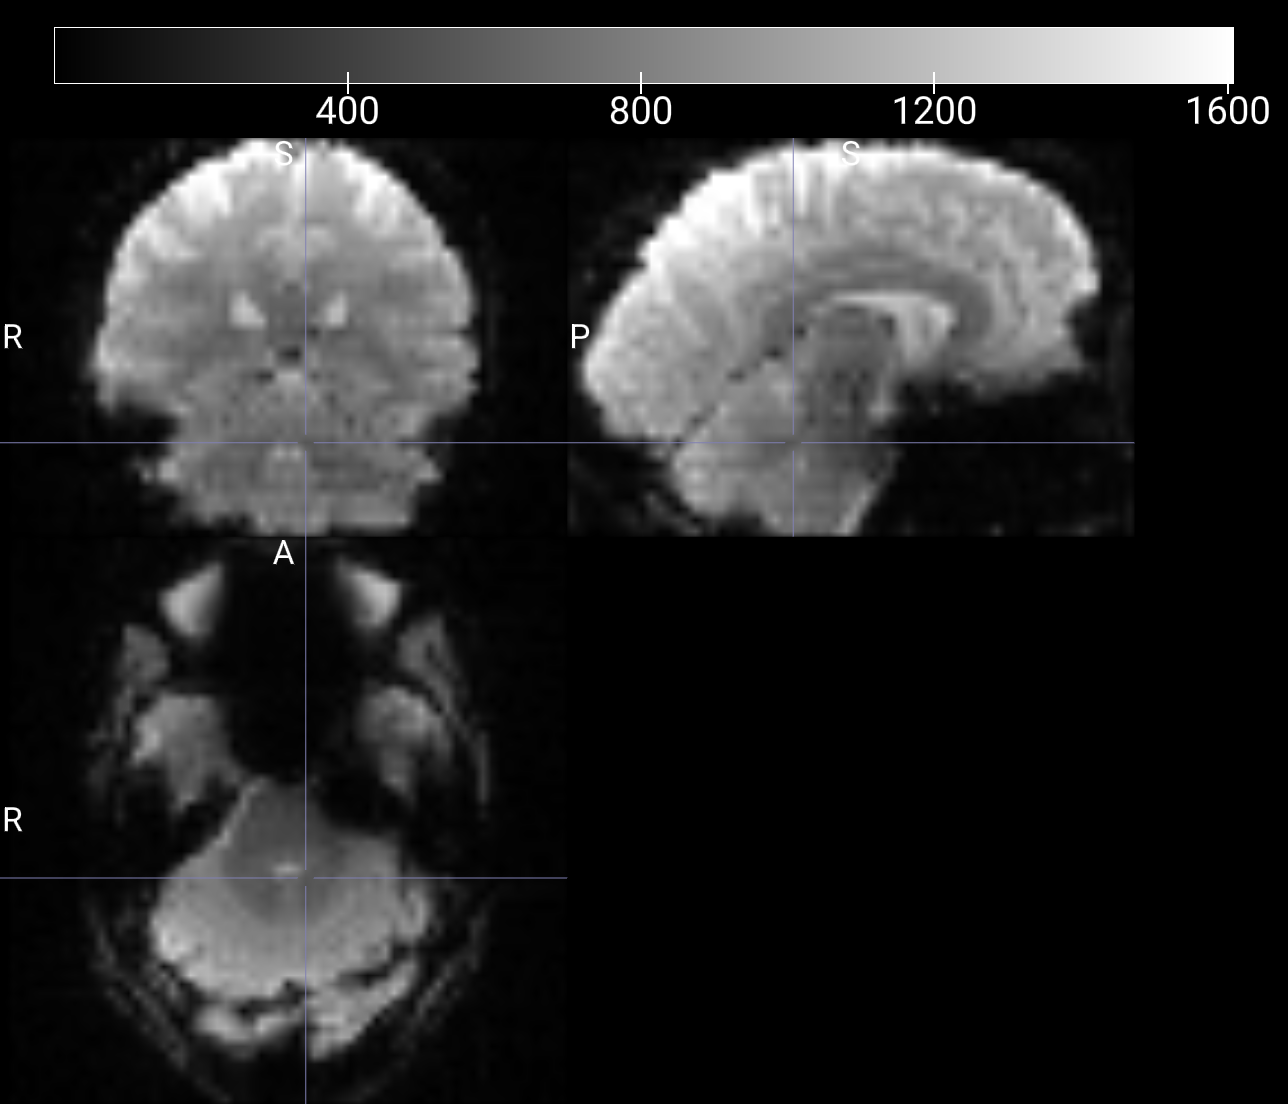
\includegraphics[width=\textwidth]{04_marco_teorico/images/bold_volume.png}
        \caption{Cortes de un volumen funcional (fMRI en estado de reposo).}
    \end{subfigure}

    \vspace{0.5em}

    \begin{subfigure}{0.85\textwidth}
        \centering
        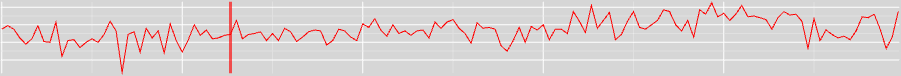
\includegraphics[width=\textwidth]{04_marco_teorico/images/bold_timeseries.png}
        \caption{Serie temporal de la señal BOLD correspondiente a un vóxel.}
    \end{subfigure}

    \caption{Ejemplo de señal BOLD en un vóxel. En la parte superior se muestran cortes del volumen funcional, y en la inferior la evolución temporal de la señal, que constituye la unidad básica para el análisis de conectividad funcional.}
    \label{fig:bold_parts}
\end{figure}


% 2.3
\section{Conectividad funcional en fMRI}
\label{sec:conectividad_funcional}

\subsection{Enfoque general de la conectividad funcional}

Como se describió en la Sección~\ref{sec:mri}, la resonancia magnética funcional permite observar la evolución temporal de la señal BOLD en distintas ubicaciones del cerebro. Cada vóxel queda asociado a una serie temporal que refleja variaciones en la oxigenación sanguínea a lo largo del tiempo.

Trabajar directamente a nivel vóxel implica manejar volúmenes tridimensionales con una cantidad muy grande de variables, lo cual resulta costoso desde el punto de vista computacional. Para dar una idea del orden de magnitud, una imagen cerebral típica tiene una resolución de aproximadamente $100 \times 100 \times 100$ vóxeles, es decir, del orden de $10^6$ variables. Si se quisiera calcular la correlación entre todos los pares de vóxeles, el número de conexiones crecería como el cuadrado del número de vóxeles, resultando en aproximadamente $10^{12}$ pares, lo cual es inviable en la práctica. Además, vóxeles espacialmente cercanos suelen presentar señales temporales similares, ya que capturan actividad proveniente de regiones anatómicamente próximas. Por este motivo, en muchos estudios no se pierde información relevante al resumir la señal a nivel regional, por ejemplo mediante el promedio de las señales de un conjunto de vóxeles que pertenecen a una misma zona.

En este contexto, la conectividad funcional se entiende como una forma de cuantificar la dependencia temporal entre regiones cerebrales anatómicamente separadas. Si las fluctuaciones de la señal BOLD de dos regiones tienden a variar de manera similar, o de forma opuesta, a lo largo del tiempo, se considera que existe conectividad funcional entre ellas \cite{van2010exploring}.

\subsection{Normalización espacial y parcelación cerebral}

Para poder comparar datos entre distintos sujetos, es necesario que las regiones cerebrales se correspondan de manera consistente entre individuos. Dado que cada cerebro presenta diferencias en forma y tamaño, en neuroimagen se utiliza un espacio de referencia común o espacio estándar que permita establecer una correspondencia anatómica entre sujetos.

Una estrategia ampliamente utilizada consiste en construir plantillas cerebrales a partir de imágenes de resonancia magnética de múltiples sujetos, las cuales son alineadas y promediadas para generar un cerebro de referencia. Un ejemplo clásico es la plantilla MNI152, construida a partir del promedio de imágenes T1 de 152 sujetos sanos por el Instituto Neurológico de Montreal. En esta plantilla, cada región anatómica se encuentra identificada con un nombre estándar, lo que permite que al transformar la imagen de un sujeto individual a este espacio de referencia, las distintas estructuras cerebrales queden asociadas de manera consistente a regiones conocidas y nombradas. Estas plantillas definen un espacio común que sirve como marco para el análisis de datos estructurales y funcionales.

En un pipeline típico de análisis, la imagen funcional se alinea espacialmente con la imagen estructural ponderada en T1 del mismo sujeto mediante un proceso de co-registración. Este paso permite que una misma región anatómica pueda identificarse de manera consistente tanto en la imagen estructural como en la funcional. Posteriormente, se aplican transformaciones espaciales (como traslaciones, rotaciones y deformaciones no lineales) para llevar ambos volúmenes al espacio estándar \cite{mandal2012structural}.

Una vez que los datos se encuentran en un espacio común, puede aplicarse un atlas o parcelación, que divide el cerebro en un conjunto finito de regiones etiquetadas. En este trabajo se utiliza el atlas \textit{Automated Anatomical Labeling} (AAL), ampliamente adoptado en estudios de neuroimagen \cite{tzourio2002automated}. El atlas AAL se encuentra disponible en distintas configuraciones; en la práctica, suele emplearse con 90 o 116 regiones. En este trabajo se utiliza la versión de 116 regiones, acorde a los datos analizados.

La Figura~\ref{fig:t1} muestra un ejemplo de imagen estructural ponderada en T1, que actúa como referencia anatómica para la co-registración de la imagen funcional y su posterior transformación al espacio estándar.

\begin{figure}[H]
    \centering
    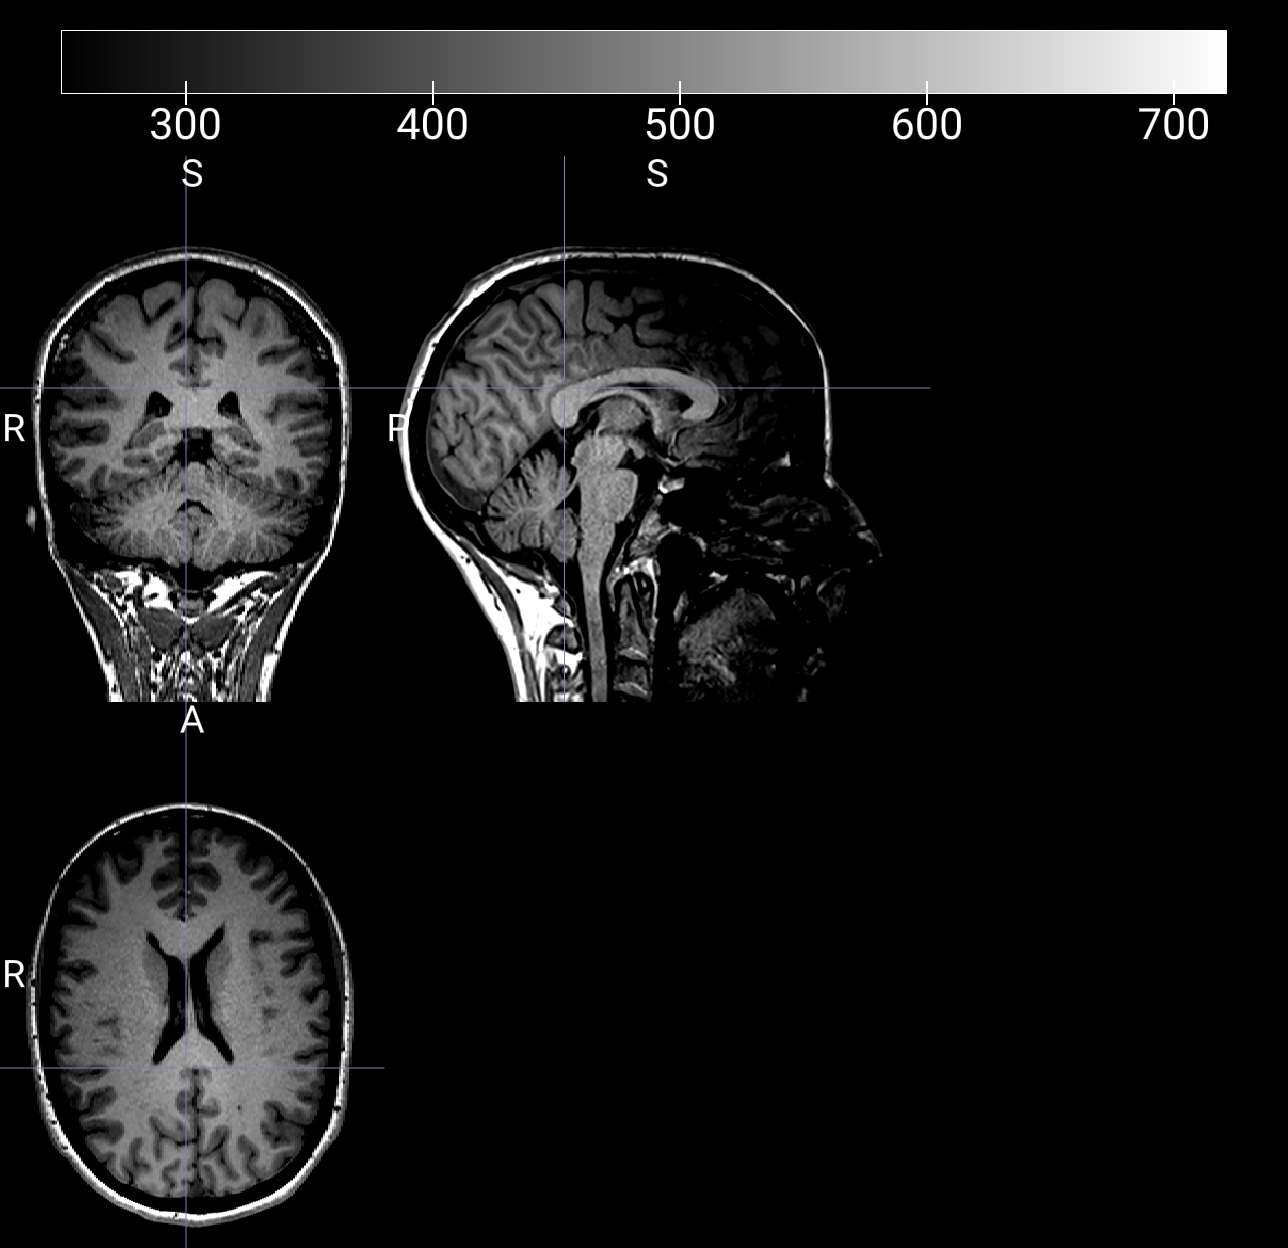
\includegraphics[width=0.85\textwidth]{04_marco_teorico/images/t1_structural.png}
    \caption{Ejemplo de imagen estructural ponderada en T1 (T1w) de un sujeto. Este volumen se utiliza como referencia anatómica para la co-registración de la imagen funcional y su posterior normalización al espacio estándar.}
    \label{fig:t1}
\end{figure}

La Figura~\ref{fig:mni} muestra el cerebro estándar MNI152 utilizado como referencia anatómica común para la alineación espacial entre sujetos. Sobre este espacio normalizado se aplica posteriormente la parcelación anatómica mediante el atlas AAL, como se ilustra en la Figura~\ref{fig:aal_mni}, donde cada color representa una región de interés (ROI) distinta.

\begin{figure}[H]
    \centering
    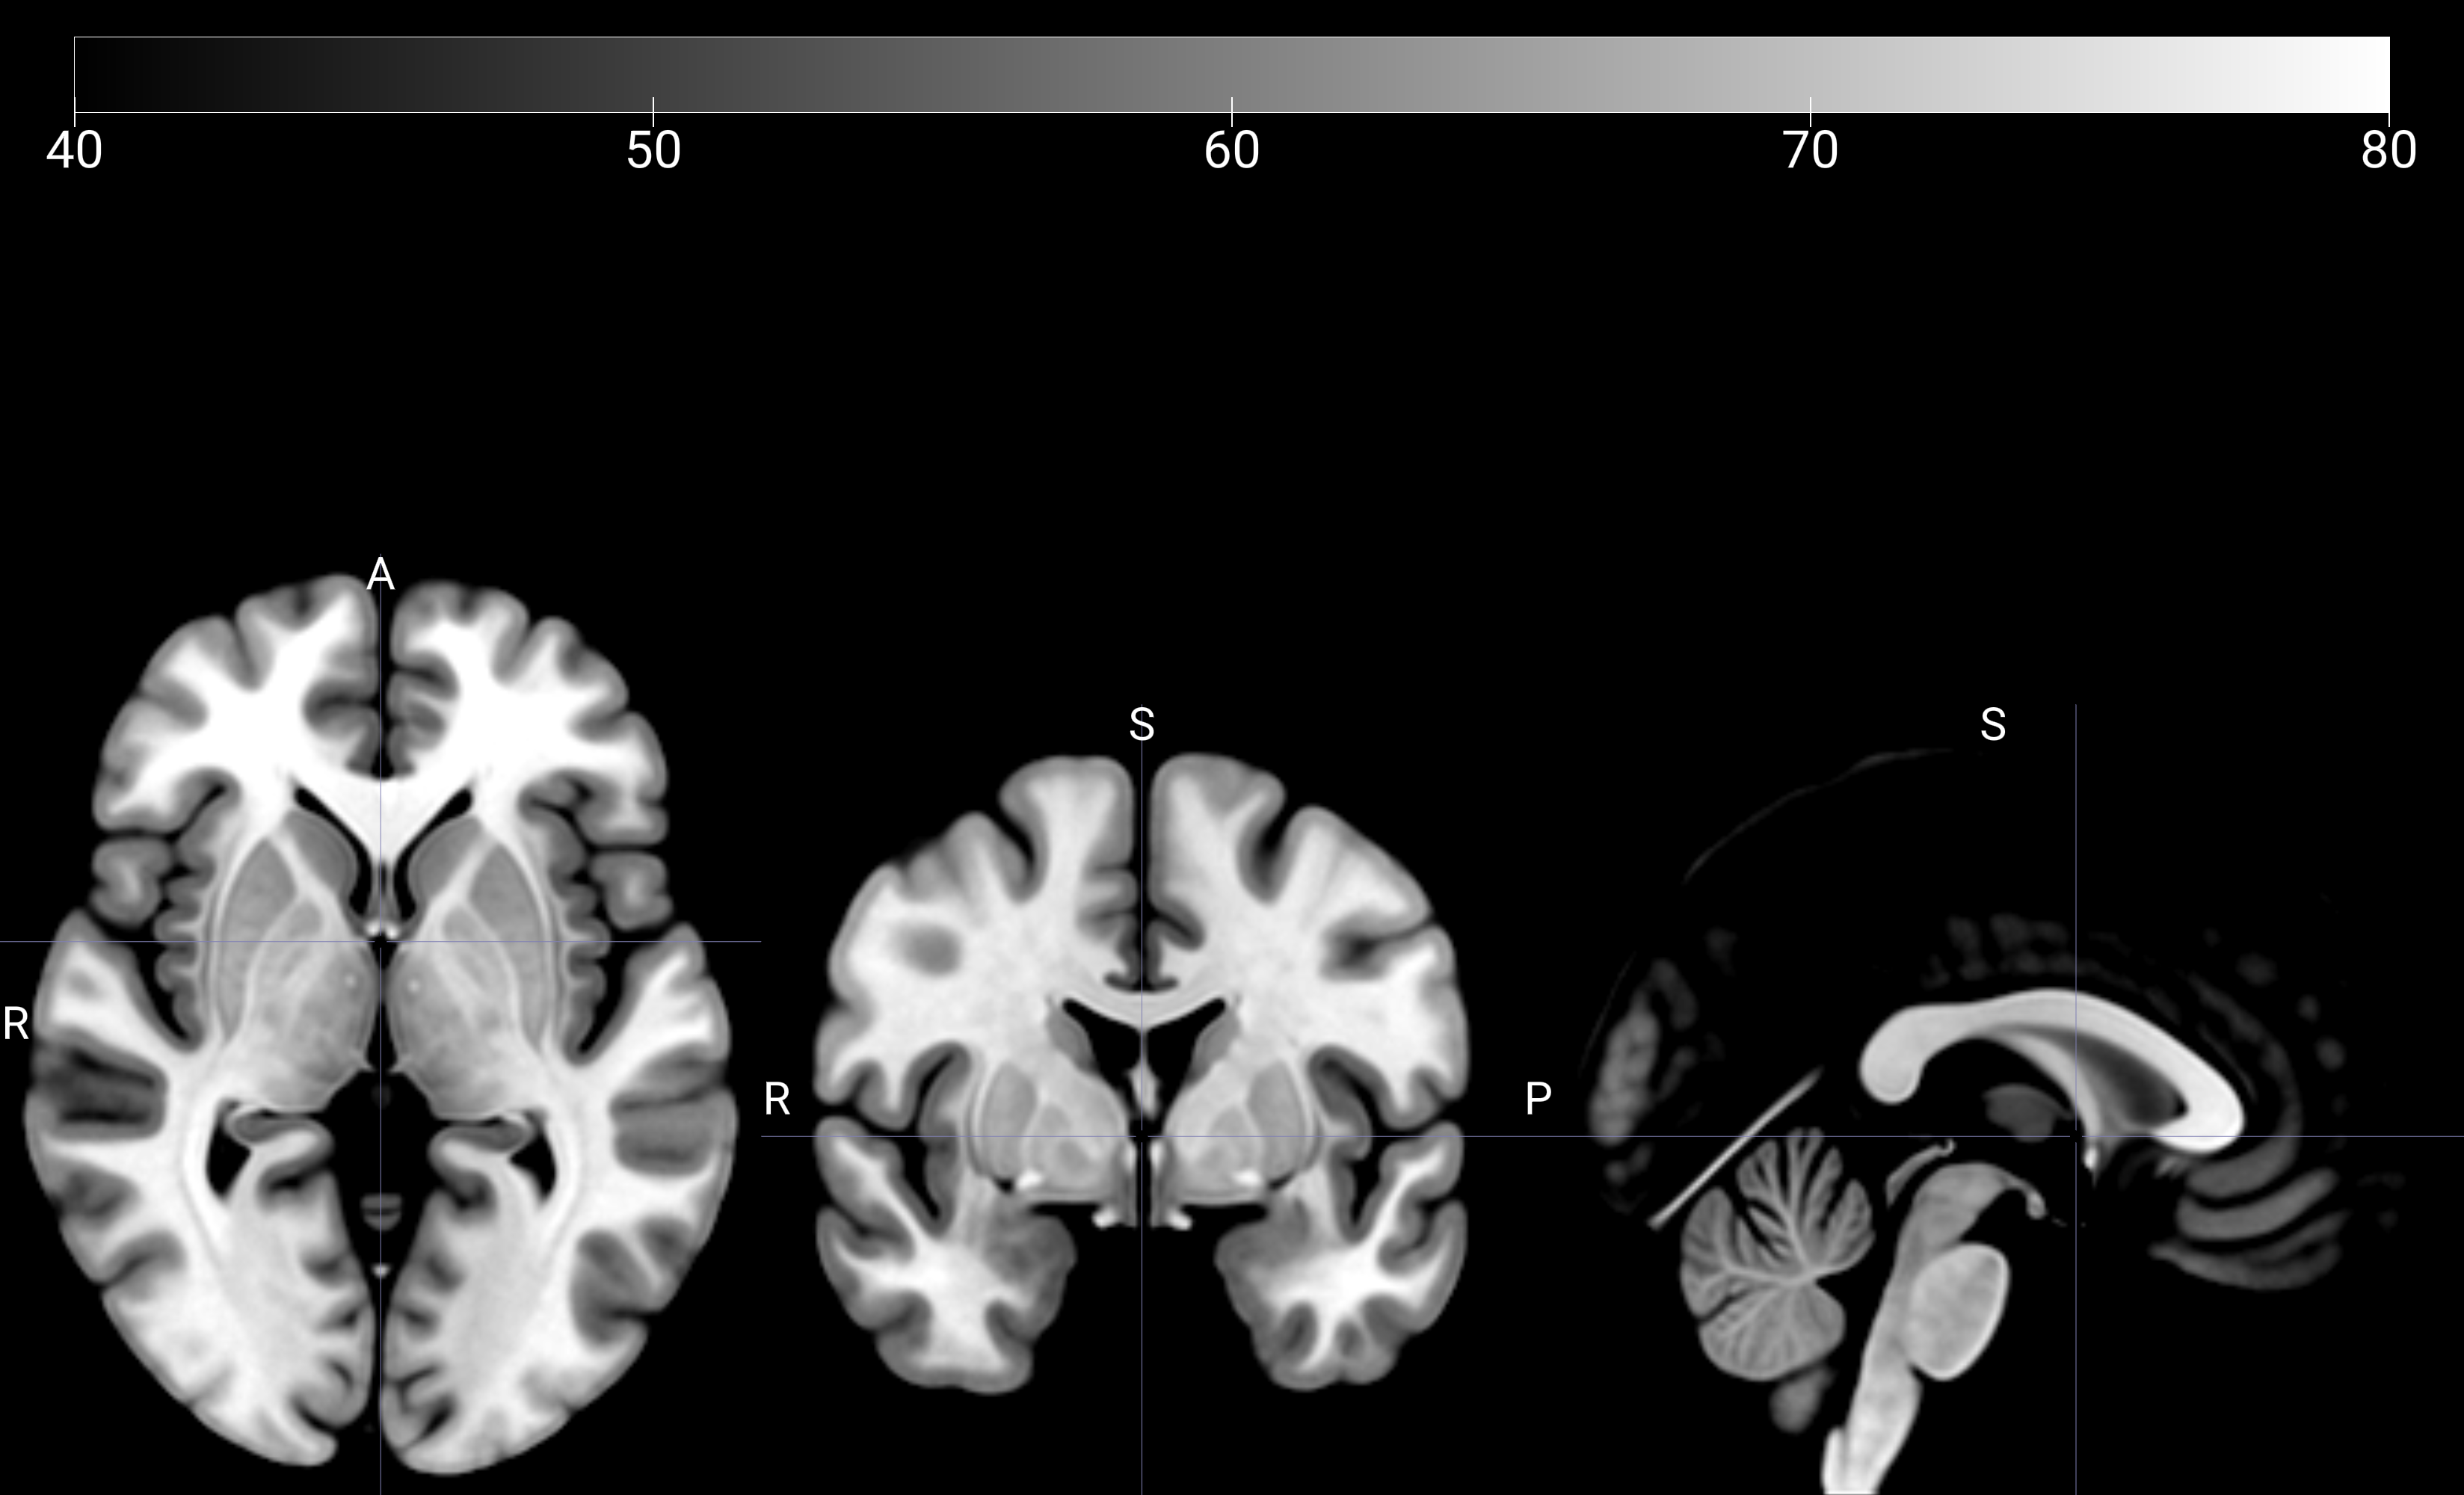
\includegraphics[width=0.85\textwidth]{04_marco_teorico/images/mni152.png}
    \caption{Cerebro estándar MNI152 en espacio normalizado, utilizado como referencia anatómica común para la alineación espacial entre sujetos.}
    \label{fig:mni}
\end{figure}

\begin{figure}[H]
    \centering
    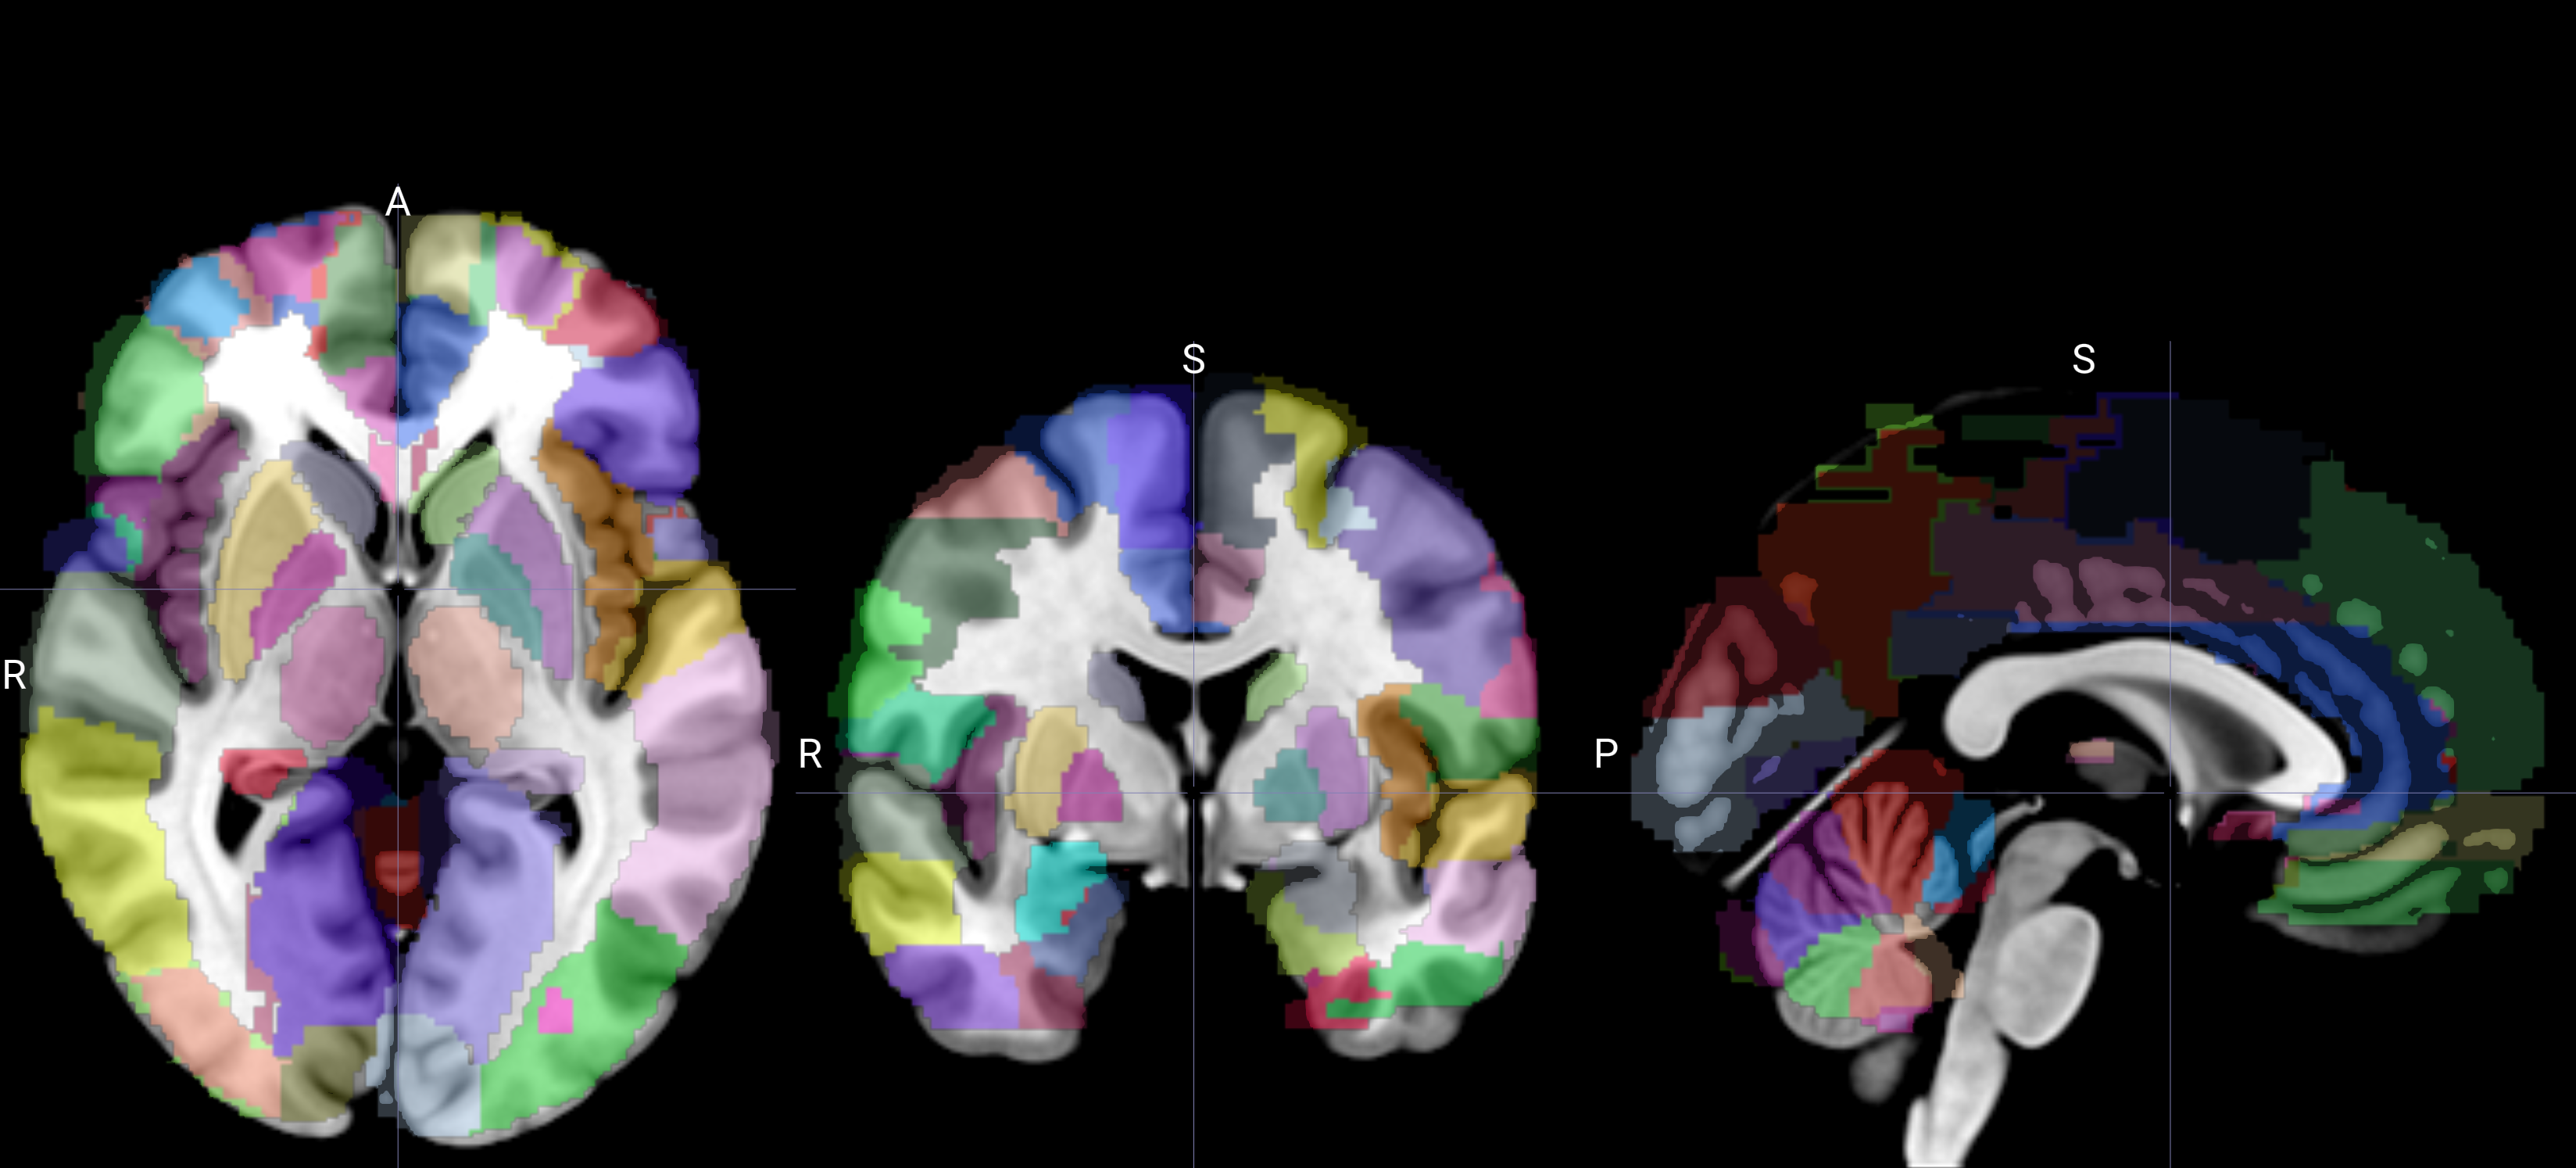
\includegraphics[width=0.85\textwidth]{04_marco_teorico/images/mni152+atlas.png}
    \caption{Atlas Automated Anatomical Labeling (AAL) superpuesto sobre el cerebro estándar MNI152. Cada color representa una región anatómica distinta utilizada como región de interés (ROI).}
    \label{fig:aal_mni}
\end{figure}


\subsection{Obtención de series temporales regionales}

Una vez aplicado el atlas, cada región agrupa múltiples vóxeles. Una forma habitual de representar la actividad de cada región consiste en construir una serie temporal regional como el promedio de las señales BOLD de los vóxeles pertenecientes a dicha región. Este procedimiento reduce significativamente la dimensionalidad de los datos y facilita el análisis posterior, manteniendo información relevante sobre la dinámica temporal de la señal \cite{shahhosseini2022functional}.

En estudios de fMRI en estado de reposo, la señal BOLD suele someterse a distintos pasos de preprocesamiento con el objetivo de reducir fuentes de ruido y mejorar la comparabilidad entre sujetos. Estos pasos incluyen correcciones asociadas al movimiento del sujeto durante la toma de imágenes, regresión de señales no neuronales y filtrado temporal. En particular, se ha observado que las fluctuaciones relevantes de la señal en estado de reposo se concentran en un rango de bajas frecuencias, típicamente del orden de 0,01–0,08 Hz \cite{smitha2017resting}.

En este trabajo se parte directamente de series temporales regionales que ya fueron obtenidas y preprocesadas como parte del procesamiento previo de los datos, por lo que no se realizan pasos adicionales de preprocesamiento a nivel vóxel.

\subsection{Estimación y representación de la conectividad funcional}

Con una serie temporal por región, la conectividad funcional se estima midiendo la dependencia estadística entre pares de regiones. Una de las medidas más utilizadas para este fin es la correlación de Pearson, debido a su simplicidad e interpretabilidad, ya que cuantifica el grado de asociación lineal entre dos series temporales \cite{van2010exploring}. Esta medida permite evaluar si dos regiones presentan fluctuaciones temporales sincronizadas o anticorrelacionadas.

La Figura~\ref{fig:ts_corr} ilustra este concepto con dos ejemplos: un par de regiones cuyas señales fluctúan de forma sincronizada (correlación positiva alta) y un par con fluctuaciones opuestas (anticorrelación).

\begin{figure}[H]
    \centering
    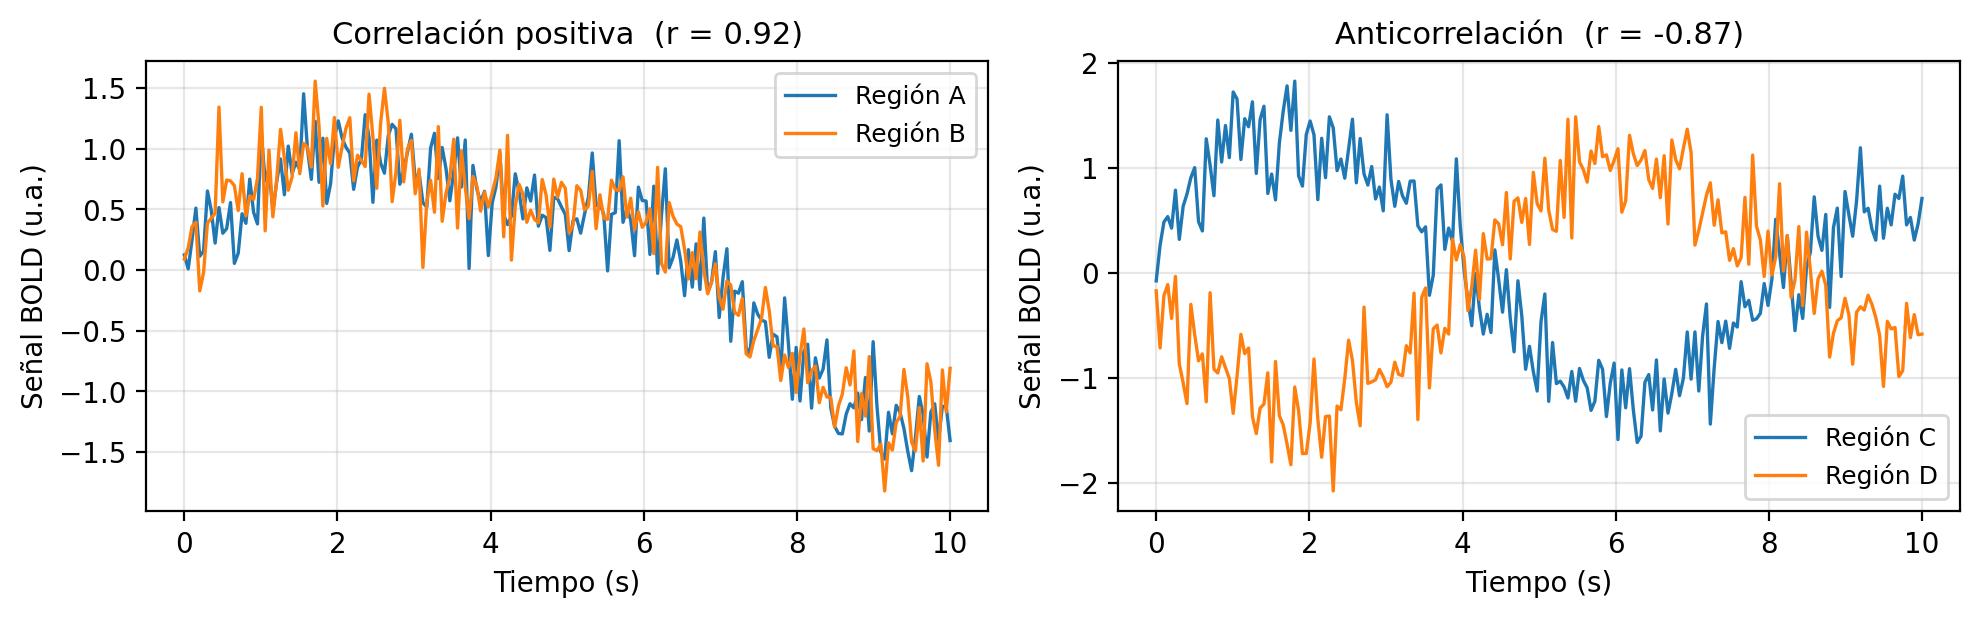
\includegraphics[width=0.95\textwidth]{04_marco_teorico/images/timeseries_correlation.png}
    \caption{Ejemplo de series temporales BOLD simuladas para dos pares de regiones cerebrales. Izquierda: regiones con correlación positiva ($r = 0{,}92$), cuyas señales fluctúan de forma sincronizada. Derecha: regiones anticorrelacionadas ($r = -0{,}87$), con fluctuaciones opuestas.}
    \label{fig:ts_corr}
\end{figure}

A partir de estas correlaciones se construye una matriz de conectividad funcional de tamaño $N \times N$, donde $N$ es el número de regiones del atlas. Cada entrada $(i,j)$ corresponde a la correlación entre la serie temporal regional de la región $i$ y la de la región $j$. Esta representación matricial constituye una forma compacta y ampliamente utilizada de describir la organización funcional del cerebro, y sirve como punto de partida para análisis posteriores basados en redes o enfoques de aprendizaje automático.

La Figura~\ref{fig:fc} muestra un ejemplo de una matriz de conectividad funcional real obtenida a partir de datos de fMRI en estado de reposo, ilustrando la estructura simétrica y los patrones de asociación entre regiones.

\begin{figure}[H]
    \centering
    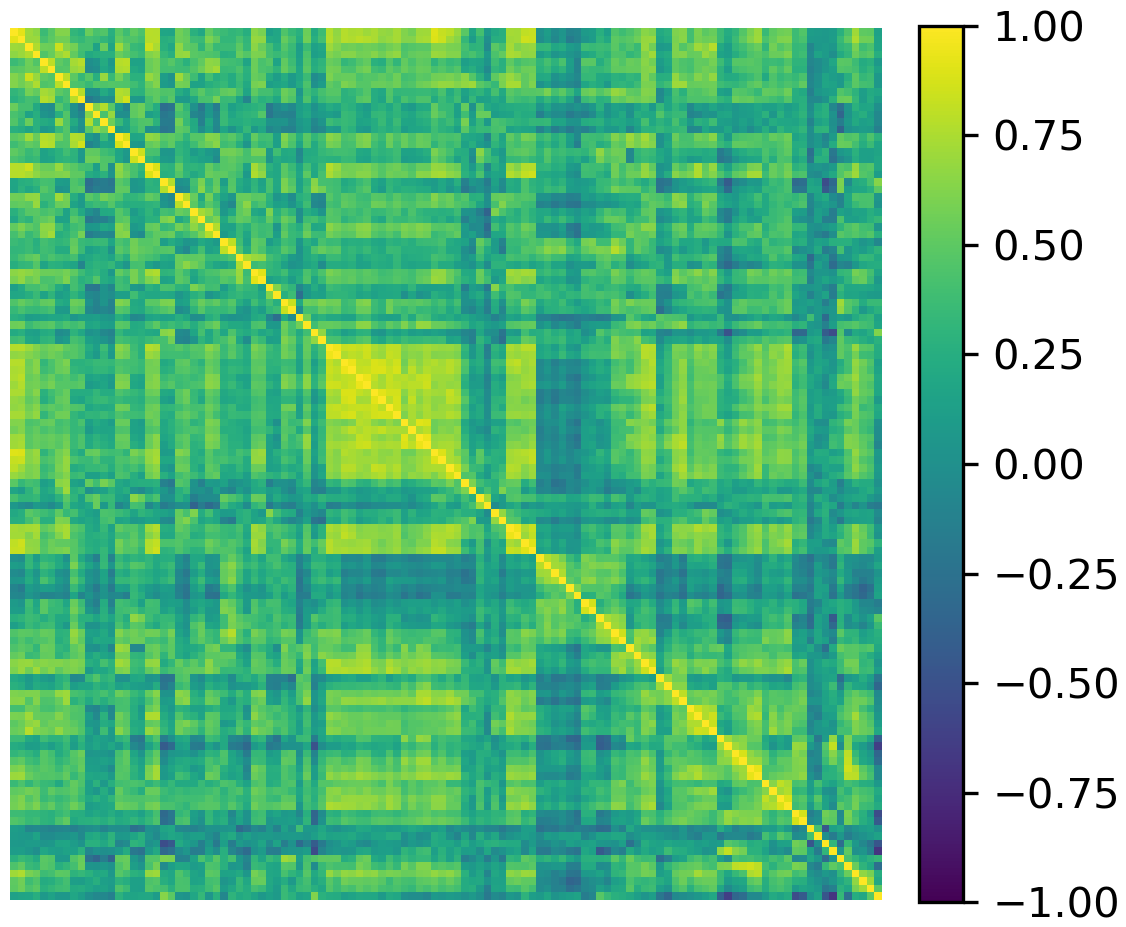
\includegraphics[width=0.6\textwidth]{04_marco_teorico/images/fc_example.png}
    \caption{Ejemplo de matriz de conectividad funcional (116×116) estimada mediante correlación de Pearson entre las series temporales regionales. Cada entrada representa el grado de asociación entre dos regiones cerebrales.}
    \label{fig:fc}
\end{figure}

\subsection{Transformación Fisher $z$}
\label{sec:fisher_z}

Los coeficientes de correlación de Pearson están acotados al intervalo $(-1, 1)$ y presentan una distribución asimétrica, particularmente para valores cercanos a los extremos. Esta propiedad puede resultar problemática para métodos estadísticos y modelos de aprendizaje automático que asumen distribuciones aproximadamente normales.

La transformación Fisher $z$ \cite{fisher1921probable} convierte los coeficientes de correlación en valores definidos sobre toda la recta real con una distribución aproximadamente normal:
\[
z_{ij} = \text{arctanh}(r_{ij}) = \frac{1}{2} \ln \left( \frac{1 + r_{ij}}{1 - r_{ij}} \right),
\]
donde $r_{ij}$ es la correlación de Pearson entre las regiones $i$ y $j$. Esta transformación es una práctica estándar en estudios de conectividad funcional y tiene la ventaja adicional de estabilizar la varianza de los coeficientes de correlación, lo que favorece la estabilidad numérica durante el entrenamiento de modelos.

%2.4

\section{Modelos computacionales y aprendizaje automático}
\label{sec:modelos_ml}

\subsection{Aprendizaje automático en neuroimagen}
Durante las últimas décadas se han producido avances significativos en el estudio del cerebro y de los trastornos neurológicos y psiquiátricos, en gran parte impulsados por el desarrollo de técnicas de neuroimagen. Tradicionalmente, el análisis de estos datos se ha basado en métodos estadísticos clásicos orientados a realizar inferencias a nivel grupal. Este enfoque consiste, en general, en comparar grupos de sujetos (por ejemplo, pacientes y controles sanos) para identificar diferencias promedio en determinadas regiones o medidas cerebrales.

Si bien estos métodos han permitido caracterizar patrones generales asociados a distintas patologías, presentan limitaciones importantes cuando se pretende realizar inferencias a nivel individual. En particular, los análisis grupales no permiten realizar predicciones sobre sujetos individuales, lo que ha dificultado la transferencia de los resultados de la investigación en neuroimagen hacia aplicaciones clínicas, como el diagnóstico personalizado o la predicción de respuesta a tratamientos \cite{mwangi2014review}.

En este contexto, el aprendizaje automático ha emergido como una herramienta clave para el análisis de datos de neuroimagen. A diferencia de los enfoques clásicos, los métodos de aprendizaje automático permiten identificar patrones complejos en los datos que distinguen sujetos sanos de pacientes, o bien subgrupos de pacientes con características clínicas diferentes. Estos métodos han demostrado ser capaces de realizar predicciones a nivel individual (es decir, estimar una variable de interés para cada sujeto por separado, en contraste con la comparación de promedios entre grupos), abriendo nuevas posibilidades para el desarrollo de herramientas de apoyo al diagnóstico y a la toma de decisiones clínicas \cite{vieira2020introduction}. Cabe señalar que esto no impide que los modelos se entrenen sobre cohortes heterogéneas que incluyan tanto sujetos sanos como pacientes; la diferencia radica en que la predicción se realiza para cada individuo.

Otra diferencia fundamental radica en el carácter multivariable del aprendizaje automático. Mientras que los enfoques estadísticos tradicionales suelen analizar una variable a la vez, los modelos de aprendizaje automático consideran simultáneamente un gran número de variables de entrada. Esto resulta especialmente relevante en neuroimagen, donde es frecuente combinar información proveniente de múltiples modalidades, como imágenes estructurales, funcionales o de difusión, con el objetivo de mejorar el poder predictivo de los modelos \cite{mwangi2014review}.

Desde un punto de vista conceptual, el objetivo del análisis también se desplaza. En lugar de formular hipótesis específicas sobre los datos y evaluarlas bajo supuestos estadísticos predefinidos, el aprendizaje automático adopta un enfoque más exploratorio, en el cual se busca que los propios datos revelen patrones y relaciones relevantes sin imponer restricciones fuertes a priori \cite{vieira2020introduction}.

\subsection{Motivación para la reducción de dimensionalidad}
Un desafío central en la aplicación de aprendizaje automático a datos de neuroimagen es la alta dimensionalidad de los datos. En muchos estudios, el número de sujetos disponibles suele ser relativamente pequeño, mientras que el número de variables (por ejemplo, vóxeles o características derivadas de las imágenes) puede superar ampliamente las decenas o cientos de miles. Esta situación, conocida como el problema de alta dimensionalidad o ``small-n large-p'', incrementa significativamente el riesgo de sobreajuste de los modelos \cite{mwangi2014review}.

El sobreajuste ocurre cuando un modelo aprende patrones específicos del conjunto de entrenamiento que no generalizan a nuevos datos, lo que se traduce en un bajo rendimiento predictivo sobre sujetos no vistos durante el entrenamiento. Para mitigar este problema, existe un amplio consenso en la literatura de neuroimagen sobre la necesidad de aplicar técnicas de reducción de dimensionalidad o selección de características antes de entrenar modelos predictivos \cite{mwangi2014review}.

Además de reducir el riesgo de sobreajuste y el costo computacional, la reducción de dimensionalidad puede contribuir a eliminar información redundante o irrelevante y facilitar una interpretación más clara de los patrones subyacentes en los datos. En este sentido, los métodos de reducción de dimensionalidad constituyen un componente fundamental en muchos pipelines de aprendizaje automático aplicados a neuroimagen.

Entre los métodos de reducción de dimensionalidad más utilizados se encuentran el Análisis de Componentes Principales (PCA), un enfoque lineal clásico, y los autoencoders variacionales, capaces de modelar relaciones no lineales. Ambos enfoques se describen a continuación.


\subsection{Análisis de Componentes Principales (PCA)}
\label{sec:pca}

El Análisis de Componentes Principales (\textit{Principal Component Analysis}, PCA) es uno de los métodos de reducción de dimensionalidad más utilizados en estadística y aprendizaje automático \cite{jolliffe2002pca}. Su objetivo es transformar un conjunto de variables posiblemente correlacionadas en un nuevo conjunto de variables no correlacionadas, denominadas \textit{componentes principales}, que resumen la información más relevante contenida en los datos originales.

La intuición detrás de PCA es sencilla: dado un conjunto de datos de alta dimensionalidad, muchas de las variables originales están correlacionadas entre sí y contienen información redundante. PCA identifica las direcciones en el espacio de datos a lo largo de las cuales la variabilidad es máxima, es decir, las direcciones que mejor distinguen entre las observaciones. La primera componente principal es la dirección de mayor varianza; la segunda es la dirección de mayor varianza restante, con la restricción de ser perpendicular a la primera; y así sucesivamente. De esta forma, las primeras $k$ componentes capturan la mayor parte de la variabilidad total de los datos, y las restantes (que contienen principalmente ruido o información redundante) pueden descartarse.

Desde el punto de vista práctico, aplicar PCA equivale a proyectar los datos originales sobre estas $k$ direcciones principales, obteniendo una representación compacta donde cada observación queda descrita por $k$ valores en lugar de los $p$ originales. Por ejemplo, en el contexto de este trabajo, una matriz de conectividad funcional representada por 6670 valores puede comprimirse a 64 componentes principales, reteniendo las fuentes de variación más informativas y descartando el resto.

PCA es un método determinista y lineal: solo puede capturar relaciones lineales entre las variables originales. Esta limitación, que lo distingue de los autoencoders (capaces de modelar dependencias no lineales), tiene como contrapartida una notable simplicidad: PCA no requiere entrenamiento iterativo, no tiene hiperparámetros más allá del número de componentes $k$, y su cálculo se obtiene directamente a partir de la estructura de covarianza de los datos \cite{jolliffe2002pca}. En el contexto de neuroimagen, PCA y sus extensiones han sido utilizados como componente de reducción de dimensionalidad en pipelines de predicción de edad cerebral a partir de conectividad funcional \cite{monti2020interpretable}, y comparaciones sistemáticas de workflows han identificado a PCA combinado con algoritmos no lineales entre las configuraciones de mejor rendimiento \cite{more2023brain}.

\subsection{Autoencoders y autoencoders variacionales}

\subsubsection{Autoencoders}

Un autoencoder es un tipo de red neuronal multicapa entrenada con el objetivo de reproducir su entrada en la salida. Su arquitectura se compone de dos módulos principales: un codificador (\textit{encoder}), que transforma los datos de entrada en una representación de menor dimensión, y un decodificador (\textit{decoder}), que intenta reconstruir la entrada original a partir de dicha representación \cite{vieira2017using,michelucci2022introduction}.

El codificador aprende una representación latente para cada dato de entrada, expresada como un vector en un espacio latente de dimensión reducida. Esta representación puede interpretarse como un punto en un espacio multidimensional de menor dimensión que el espacio original. De este modo, una entrada originalmente descrita por un gran número de variables es transformada en una representación compacta que captura patrones o información relevante de los datos originales.

Desde el punto de vista del aprendizaje, los autoencoders se entrenan de manera no supervisada, ya que no requieren datos etiquetados. El propio conjunto de datos de entrada actúa como referencia durante el entrenamiento, dado que el objetivo del modelo es minimizar la diferencia entre la entrada y su reconstrucción. Esta diferencia se cuantifica mediante un error de reconstrucción, que mide qué tan fiel es la salida del modelo con respecto al dato original. Una de las métricas más utilizadas para este fin es el error cuadrático medio (MSE), definido como
\[
MSE = \frac{1}{N} \sum_{i=1}^{N} (x_i - \tilde{x}_i)^2.
\]
Un valor elevado del error de reconstrucción indica que el modelo no ha logrado capturar adecuadamente la estructura de los datos, mientras que un valor reducido sugiere que la representación latente aprendida permite reconstrucciones precisas \cite{michelucci2022introduction}. Otra métrica frecuente es el error absoluto medio (MAE), más robusta ante valores atípicos. En este trabajo se utiliza MAE como pérdida de reconstrucción (véase Capítulo~\ref{chapter:metodologia_pipeline}).

Una característica fundamental de los autoencoders es la presencia de un cuello de botella (\textit{bottleneck}) en el espacio latente, que fuerza al modelo a reducir progresivamente la dimensionalidad de los datos a través de capas intermedias con un número decreciente de unidades. Esta restricción obliga al modelo a aprender representaciones informativas, ya que solo puede preservar la información más relevante para reconstruir adecuadamente la entrada. Por este motivo, los autoencoders son utilizados frecuentemente como extractores de características en distintos contextos, incluyendo aplicaciones de neuroimagen \cite{vieira2017using}.

La dimensionalidad del espacio latente constituye un compromiso central en el diseño de un autoencoder. Un espacio latente excesivamente pequeño puede limitar la capacidad del modelo para capturar características relevantes de los datos, lo que se traduce en reconstrucciones imprecisas. Por el contrario, un espacio latente demasiado grande puede reducir la efectividad del cuello de botella, permitiendo representaciones poco informativas y afectando la organización del espacio latente. En la práctica, una mala calidad de reconstrucción suele estar asociada a un espacio latente desestructurado, donde las representaciones aprendidas no reflejan adecuadamente las relaciones entre los datos.

En comparación con PCA (Sección~\ref{sec:pca}), los autoencoders presentan ciertas ventajas prácticas. En particular, pueden entrenarse utilizando mini-batches, lo que los hace adecuados para trabajar con grandes volúmenes de datos, mientras que PCA requiere procesar el conjunto completo de datos para estimar la transformación. Además, al utilizar funciones de activación no lineales, los autoencoders pueden modelar relaciones más complejas entre las variables de entrada, lo que puede resultar beneficioso en contextos donde los datos presentan estructuras no triviales. Sin embargo, esta mayor expresividad tiene un costo: los autoencoders introducen múltiples hiperparámetros (número de capas, dimensiones, tasa de aprendizaje, regularización) que requieren ser optimizados, mientras que PCA solo requiere la elección del número de componentes $k$.

La Figura~\ref{fig:ae_arch} esquematiza la arquitectura general de un autoencoder convencional.

\begin{figure}[H]
\centering
\shorthandoff{>}
\begin{tikzpicture}[
    >=Stealth,
    neuron/.style={circle, draw, thick, minimum size=0.55cm, inner sep=0pt},
    input/.style={neuron, fill=teal!20},
    hidden/.style={neuron, fill=blue!15},
    latent/.style={neuron, fill=orange!25},
    output/.style={neuron, fill=teal!20},
    conn/.style={-, gray!50, thin},
    arr/.style={->, thick},
    brace/.style={decorate, decoration={brace, amplitude=5pt, mirror}},
]

% --- Input layer (5 neurons) ---
\foreach \i in {1,...,5} {
    \node[input] (in\i) at (0, -\i*0.8 + 2.4) {};
}
\node[above=0.15cm of in1, font=\small\bfseries] {$\mathbf{x}$};

% --- Encoder hidden layer (3 neurons) ---
\foreach \i in {1,...,3} {
    \node[hidden] (h1\i) at (2.2, -\i*0.8 + 1.6) {};
}

% --- Latent layer (2 neurons) ---
\foreach \i in {1,...,2} {
    \node[latent] (z\i) at (4.4, -\i*0.8 + 1.2) {};
}
\node[above=0.15cm of z1, font=\small\bfseries] {$\mathbf{z}$};
\node[below=0.3cm of z2, font=\footnotesize, gray] (kdims) {$k$ dims};

% --- Decoder hidden layer (3 neurons) ---
\foreach \i in {1,...,3} {
    \node[hidden] (h2\i) at (6.6, -\i*0.8 + 1.6) {};
}

% --- Output layer (5 neurons) ---
\foreach \i in {1,...,5} {
    \node[output] (out\i) at (8.8, -\i*0.8 + 2.4) {};
}
\node[above=0.15cm of out1, font=\small\bfseries] {$\tilde{\mathbf{x}}$};

% --- Connections: input -> hidden1 ---
\foreach \i in {1,...,5} {
    \foreach \j in {1,...,3} {
        \draw[conn] (in\i) -- (h1\j);
    }
}
% --- Connections: hidden1 -> latent ---
\foreach \i in {1,...,3} {
    \foreach \j in {1,...,2} {
        \draw[conn] (h1\i) -- (z\j);
    }
}
% --- Connections: latent -> hidden2 ---
\foreach \i in {1,...,2} {
    \foreach \j in {1,...,3} {
        \draw[conn] (z\i) -- (h2\j);
    }
}
% --- Connections: hidden2 -> output ---
\foreach \i in {1,...,3} {
    \foreach \j in {1,...,5} {
        \draw[conn] (h2\i) -- (out\j);
    }
}

% --- Braces and labels ---
\draw[decorate, decoration={brace, amplitude=5pt}]
    (-0.65, -2.0) -- (-0.65, 2.0)
    node[midway, left=6pt, font=\footnotesize, align=center] {$d$\\dims};
\draw[decorate, decoration={brace, amplitude=5pt, mirror}]
    (9.45, -2.0) -- (9.45, 2.0)
    node[midway, right=6pt, font=\footnotesize, align=center] {$d$\\dims};

% --- Encoder / Decoder labels ---
\node[font=\footnotesize, gray] at (1.1, -2.8) {Encoder};
\node[font=\footnotesize, gray] at (7.7, -2.8) {Decoder};
\draw[gray, dashed, rounded corners] (-0.6, -2.5) rectangle (5.0, 2.8);
\draw[gray, dashed, rounded corners] (3.8, -2.5) rectangle (9.4, 2.8);

% --- Latent space mini-plot ---
\begin{scope}[shift={(4.4, -4.2)}]
    % Axes
    \draw[->, thick] (-1.1, 0) -- (1.3, 0) node[right, font=\scriptsize] {$z_1$};
    \draw[->, thick] (0, -0.9) -- (0, 1.3) node[above, font=\scriptsize] {$z_2$};
    % Scattered points (other data points, light)
    \foreach \px/\py in {-0.7/0.3, -0.4/-0.5, 0.2/0.8, 0.6/-0.3, 0.9/0.5,
                         -0.3/0.7, 0.5/0.1, -0.8/-0.2, 0.1/-0.7, 0.7/0.9} {
        \fill[blue!25] (\px, \py) circle (1.5pt);
    }
    % Highlighted point
    \fill[orange!80!red] (0.35, 0.45) circle (3pt);
    \draw[-{Stealth[length=1.8mm]}, orange!80!red, semithick] (0.47, 0.53) -- ++(0.25, 0.18)
        node[right, font=\scriptsize] {$\mathbf{z}_i$};
    % Label
    \node[below=0.2cm, font=\scriptsize, gray] at (0, -0.9) {Espacio latente};
\end{scope}

% --- Arrow from latent neurons to mini-plot ---
\draw[->, dashed, gray] (kdims.south) -- ++(0, -0.8);

% --- Loss below ---
\node[font=\small] at (4.4, -6.5) {$\mathcal{L}_{\text{rec}}(\mathbf{x}, \tilde{\mathbf{x}})$};

\end{tikzpicture}
\shorthandon{>}
\caption{Arquitectura de un autoencoder convencional. La entrada $\mathbf{x}$ de dimensión $d$ es comprimida por el encoder a trav\'es de capas ocultas sucesivamente menores hasta una representación latente $\mathbf{z}$ de baja dimensión (cuello de botella). El decoder reconstruye la entrada original como $\tilde{\mathbf{x}}$. El mini-gráfico inferior ilustra el espacio latente bidimensional, donde cada punto naranja representa la codificación de un dato de entrada. El modelo se entrena minimizando $\mathcal{L}_{\text{rec}}$.}
\label{fig:ae_arch}
\end{figure}

\subsubsection{Autoencoders variacionales (VAE)}

Los autoencoders clásicos, si bien efectivos para reducir dimensionalidad, no imponen restricciones explícitas sobre la organización global del espacio latente. Como consecuencia, dicho espacio puede resultar irregular o fragmentado, de modo que tomar puntos arbitrarios y decodificarlos conduce, en muchos casos, a reconstrucciones poco significativas o dominadas por ruido. Idealmente, sería deseable que puntos cercanos en el espacio latente correspondan a datos similares, y que interpolaciones suaves entre representaciones latentes produzcan variaciones plausibles de los datos originales \cite{doersch2016tutorial}.

Los autoencoders variacionales (VAE) fueron propuestos originalmente por Kingma y Welling en el trabajo \textit{Auto-Encoding Variational Bayes} \cite{kingma2013auto} con el objetivo de abordar esta limitación mediante la introducción de una formulación probabilística del espacio latente. A diferencia de los autoencoders clásicos, que codifican cada entrada en un único vector latente determinista, un VAE asocia a cada dato de entrada $x$ una distribución de probabilidad sobre variables latentes $z$. Esta representación probabilística introduce incertidumbre controlada y permite imponer una estructura explícita sobre el espacio latente, favoreciendo su regularidad y continuidad \cite{kingma2019introduction}.

En este marco, se define una distribución latente $p(z)$, denominada \textit{prior}, a partir de la cual se busca generar representaciones latentes que luego puedan decodificarse para obtener observaciones en el espacio de datos. En términos generales, el objetivo de un VAE es aprender un modelo generativo capaz de producir datos plausibles similares a los observados en el conjunto de entrenamiento. Sin embargo, la distribución real de los datos $p(x)$ es desconocida y solo se dispone de muestras observadas, lo que impide su modelado directo \cite{kingma2019introduction}.

Para conectar el espacio latente con el espacio de datos, se consideran dos distribuciones condicionales. Por un lado, la distribución de verosimilitud $p(x|z)$ modela la probabilidad de observar un dato $x$ dado un vector latente $z$, y puede interpretarse como el mecanismo de decodificación desde el espacio latente hacia el espacio original. Por otro lado, la distribución posterior $p(z|x)$ describe qué valores latentes son compatibles con un dato observado $x$. En la práctica, esta distribución posterior resulta intratable, por lo que se introduce un modelo de inferencia aproximado $q(z|x)$, también denominado codificador o modelo de reconocimiento, que aproxima la posterior verdadera \cite{kingma2019introduction,doersch2016tutorial}.

En los VAEs se asume habitualmente un prior simple y conocido, típicamente una distribución normal estándar,
\[
p(z) = \mathcal{N}(0, I),
\]
y se aproxima la posterior mediante una distribución gaussiana cuyos parámetros dependen de la entrada:
\[
q(z|x) = \mathcal{N}\big(\mu(x), \sigma^2(x)\big).
\]
De este modo, el codificador no produce directamente un único vector latente determinista, sino los parámetros $\mu(x)$ y $\sigma(x)$ que definen una distribución latente asociada a cada dato. Esta distribución constituye la representación latente del dato en el VAE. A partir de ella, se obtiene un vector latente $z$ mediante muestreo, que es utilizado por el decodificador para reconstruir o generar una salida $\tilde{x}$.


Desde el punto de vista de la optimización, el entrenamiento de un VAE no se limita a minimizar una pérdida de reconstrucción, como ocurre en los autoencoders clásicos. La función objetivo incorpora además un término de regularización que promueve que la distribución latente aproximada $q(z|x)$ permanezca cercana al prior $p(z)$. Este término se expresa mediante la divergencia de Kullback--Leibler (KL), que mide la discrepancia entre dos distribuciones de probabilidad. La combinación de ambos objetivos se formaliza a través del criterio conocido como \textit{Evidence Lower Bound} (ELBO), que permite entrenar el modelo equilibrando la calidad de la reconstrucción con la regularización del espacio latente \cite{kingma2013auto}.
\[
\mathcal{L}_{VAE} =
\mathcal{L}_{rec}(x, \tilde{x}) +
D_{KL}\big(q(z|x)\,\|\,p(z)\big).
\]
La pérdida de reconstrucción $\mathcal{L}_{rec}$ evalúa qué tan fiel es la reconstrucción respecto a la entrada original, mientras que el término KL actúa como regularizador del espacio latente, favoreciendo representaciones continuas y bien organizadas \cite{doersch2016tutorial}.

Un aspecto fundamental en el entrenamiento de los VAEs es que la obtención del vector latente implica un proceso de muestreo, lo cual introduce aleatoriedad en el flujo de cómputo. En particular, cuando el vector latente se obtiene muestreando directamente de una distribución cuyos parámetros dependen de la entrada, dicha operación deja de ser una función determinista de los parámetros del modelo. Esto impide la propagación directa de gradientes, ya que el muestreo no es una operación diferenciable respecto a dichos parámetros.

Para resolver este inconveniente, se utiliza el denominado truco de reparametrización, que permite separar la fuente de aleatoriedad de los parámetros del modelo y expresar el muestreo de manera diferenciable \cite{kingma2013auto}. En lugar de muestrear directamente desde la distribución latente, se introduce una variable aleatoria auxiliar $\epsilon \sim \mathcal{N}(0, I)$, independiente de los parámetros aprendidos, y se define el vector latente como
\[
z = \mu(x) + \sigma(x) \odot \epsilon,
\]
donde $\mu(x)$ y $\sigma(x)$ son funciones deterministas producidas por el codificador. De este modo, la aleatoriedad queda concentrada en $\epsilon$, mientras que la transformación que genera $z$ es diferenciable respecto a los parámetros del modelo, preservando la posibilidad de entrenar el VAE mediante backpropagation.

La Figura~\ref{fig:vae_arch} resume la arquitectura de un VAE, incluyendo el truco de reparametrización.

\begin{figure}[H]
\centering
\shorthandoff{>}%
\begin{tikzpicture}[
    >=Stealth,
    block/.style={draw, thick, rounded corners=3pt, minimum height=1cm,
                  minimum width=1.6cm, fill=#1!12, font=\small, align=center},
    block/.default=blue,
    circ/.style={draw, thick, circle, minimum size=0.85cm, fill=#1!15, font=\normalsize},
    circ/.default=orange,
    arr/.style={->, thick},
]

% --- Nodes (compact layout) ---
\node (x) {$x$};
\node[block=blue, right=0.8cm of x] (enc) {Encoder\\[-2pt]{\footnotesize $q(z \mid x)$}};
\node[circ=yellow, above right=0.6cm and 1.3cm of enc] (mu) {$\boldsymbol{\mu}$};
\node[circ=orange, below right=0.6cm and 1.3cm of enc] (sigma) {$\boldsymbol{\sigma}$};
\node[circ=green, right=3.6cm of enc] (z) {$z$};
\node[block=red, right=1.2cm of z] (dec) {Decoder\\[-2pt]{\footnotesize $p(x \mid z)$}};
\node[right=0.8cm of dec] (xhat) {$\tilde{x}$};

% Epsilon node
\node[below=0.6cm of z, font=\small] (eps) {$\epsilon \sim \mathcal{N}(0, I)$};

% --- Arrows ---
\draw[arr] (x) -- (enc);
\draw[arr] (enc) |- (mu);
\draw[arr] (enc) |- (sigma);
\draw[arr] (mu) -- (z);
\draw[arr] (sigma) -- (z);
\draw[arr, dashed] (eps) -- (z);
\draw[arr] (z) -- (dec);
\draw[arr] (dec) -- (xhat);

% --- Reparameterization label ---
\node[above=0.1cm of z, font=\footnotesize\itshape] {$z = \mu + \sigma \odot \epsilon$};

% --- Loss ---
\node[below=1.5cm of z, xshift=-0.3cm, font=\small] {
    $\mathcal{L} = \underbrace{\mathcal{L}_{\text{rec}}(x,\, \tilde{x})}_{\text{\scriptsize reconstrucci\'on}}
    + \underbrace{D_{\text{KL}}\!\big(q(z|x) \,\|\, p(z)\big)}_{\text{\scriptsize regularizaci\'on}}$
};

\end{tikzpicture}%
\shorthandon{>}
\caption{Arquitectura de un autoencoder variacional (VAE). El encoder produce los parámetros $\mu$ y $\sigma$ de la distribución latente. El vector $z$ se obtiene mediante el truco de reparametrización ($z = \mu + \sigma \odot \epsilon$, con $\epsilon$ muestreado de una normal estándar), y el decoder reconstruye la entrada a partir de $z$. La función de pérdida combina un término de reconstrucción con la divergencia KL.}
\label{fig:vae_arch}
\end{figure}

\subsubsection{$\beta$-VAE}
\label{sec:beta_vae_theory}

El $\beta$-VAE \cite{higgins2017beta} es una extensión del autoencoder variacional que introduce un hiperparámetro $\beta > 0$ para ponderar explícitamente la contribución de la divergencia KL en la función de pérdida:
\[
\mathcal{L}_{\beta\text{-VAE}} = \mathcal{L}_{\text{rec}}(x, \tilde{x}) + \beta \cdot D_{\text{KL}}\big(q(z|x) \,\|\, p(z)\big).
\]

Cuando $\beta = 1$ se recupera el VAE estándar. Valores de $\beta > 1$ imponen mayor regularización sobre el espacio latente, promoviendo representaciones más regulares y desentrelazadas (\textit{disentangled}), a costa de una peor reconstrucción. Valores de $\beta < 1$ relajan la restricción, priorizando la calidad de la reconstrucción.

Este hiperparámetro permite ajustar explícitamente el compromiso entre fidelidad de reconstrucción y regularidad del espacio latente, lo que resulta particularmente útil cuando las representaciones latentes se utilizan como entrada para una tarea posterior (\textit{downstream task}). En tales casos, el valor óptimo de $\beta$ depende de la naturaleza de la tarea y de los datos, y puede ser determinado mediante técnicas de optimización de hiperparámetros.

\paragraph{Calentamiento de $\beta$ (warmup).}
Un problema conocido en el entrenamiento de VAEs es el denominado \textit{colapso posterior} (\textit{posterior collapse}): si desde las primeras épocas la divergencia KL penaliza fuertemente las representaciones latentes, el encoder puede aprender a ignorar la entrada y producir distribuciones cercanas al prior, resultando en reconstrucciones deficientes. Para mitigar este fenómeno, se utiliza una estrategia de calentamiento lineal en la que $\beta$ crece progresivamente desde 0 hasta su valor objetivo durante las primeras $W$ épocas de entrenamiento:
\[
\beta(t) = \min\!\left(1, \; \frac{t}{W}\right) \cdot \beta_{\text{target}},
\]
donde $t$ denota la época de entrenamiento actual. Esto permite que el modelo aprenda primero a reconstruir los datos antes de que la regularización KL comience a estructurar el espacio latente.

\subsection{Modelos basados en árboles y boosting}

\subsubsection{Árboles de decisión para regresión}

Un árbol de decisión es un modelo que construye una secuencia de divisiones
sobre los datos con el objetivo de separar el espacio de entrada en regiones
cada vez más homogéneas. Estas divisiones se organizan en forma de árbol,
donde cada nodo interno representa una condición sobre alguna variable de
entrada, y cada rama indica el resultado de dicha condición
\cite{breiman2017classification, loh2011classification}. Más adelante se
presenta un ejemplo geométrico que ilustra visualmente cómo estas divisiones
inducen regiones con predicciones constantes.

Cuando el objetivo es predecir un valor numérico continuo, como la edad,
se habla de \textit{árboles de regresión}. En este caso, cada hoja del árbol
almacena un valor real que corresponde a la predicción asignada a todos los
datos que caen en esa región del espacio.

Los árboles de regresión se construyen de manera \textit{top--down}. El
algoritmo comienza con todos los datos en un único nodo (nodo raíz) y, de
forma recursiva, busca dividir el conjunto en dos grupos mediante una
condición simple sobre alguna de las variables. Este proceso continúa hasta
que se alcanzan nodos suficientemente homogéneos o se cumple algún criterio
de parada, como una profundidad máxima o un número mínimo de observaciones
por nodo \cite{loh2011classification}.

La idea central es particionar el espacio de datos de forma que, dentro de
cada región, los valores de la variable a predecir sean lo más similares
posible. De este modo, el árbol define una aproximación por partes,
asignando una predicción constante en cada región.

\paragraph{Predicción.}
Para predecir el valor asociado a un nuevo dato, se recorre el árbol obtenido desde la
raíz siguiendo las divisiones correspondientes hasta alcanzar una hoja. El
valor almacenado en dicha hoja se toma como predicción, y corresponde al
promedio de los valores observados en los datos que llegaron a esa hoja
durante el entrenamiento.

\paragraph{Criterio de división.}
En los árboles de regresión clásicos, como AID y CART, la impureza de un nodo
mide cuán dispersos son los valores objetivo dentro de ese nodo: es baja si
los valores son similares, y alta si presentan gran variabilidad
\cite{breiman2017classification}. En este contexto, la impureza se cuantifica
mediante la \textit{suma de errores cuadráticos} (SSE):

\[
\text{SSE} = \sum_{i=1}^{n} (y_i - \bar{y})^2,
\]

donde $y_i$ son los valores reales y $\bar{y}$ su promedio. Dado que
$\text{SSE} = n \cdot \text{Var}$, minimizar la SSE es equivalente a
minimizar la varianza del nodo, por lo que ambos criterios producen
exactamente las mismas divisiones \cite{loh2011classification}.

Para evaluar una posible división (o \textit{split}), se calcula la reducción
de impureza como la diferencia entre la SSE del nodo padre y la suma de las
SSE de los nodos hijos:

\[
\Delta = \text{SSE(padre)} - \sum_j \text{SSE(hijo}_j),
\]

y se selecciona el corte que maximiza este valor.

\paragraph{Selección del mejor predictor.}
Cuando se dispone de múltiples variables de entrada, el algoritmo evalúa
posibles divisiones para cada una de ellas. Por ejemplo, en un problema
inmobiliario con variables como \textit{superficie} y \textit{cantidad de
habitaciones}, el modelo puede proponer
reglas del tipo \textit{superficie} $< 80$ o \textit{habitaciones} $\ge 3$, 
y evaluar cuál produce la mayor reducción de impureza de la variable que se 
desea predecir. El nodo raíz se elige como aquel que genera la mayor mejora, 
y el procedimiento se repite recursivamente en cada subregión.

\paragraph{Carácter greedy.}
Los árboles de decisión siguen una estrategia \textit{greedy}: cada división
se elige de forma local, maximizando la mejora inmediata, sin reconsiderar
decisiones previas. Este enfoque no garantiza una solución globalmente
óptima, pero permite construir modelos eficientes y de bajo costo
computacional \cite{breiman2017classification}.

\medskip

\paragraph{Ejemplo geométrico (visualización del proceso).}
A continuación se presenta un ejemplo bidimensional que permite observar
de forma explícita cómo estos conceptos teóricos se materializan en una
partición concreta del espacio de entrada. Se consideran dos variables de
entrada (TV y Radio) y una variable objetivo continua (Sales), donde TV y
Radio representan el presupuesto invertido en publicidad en televisión y
radio, respectivamente, y Sales corresponde a las ventas observadas.

\begin{figure}[H]
\centering
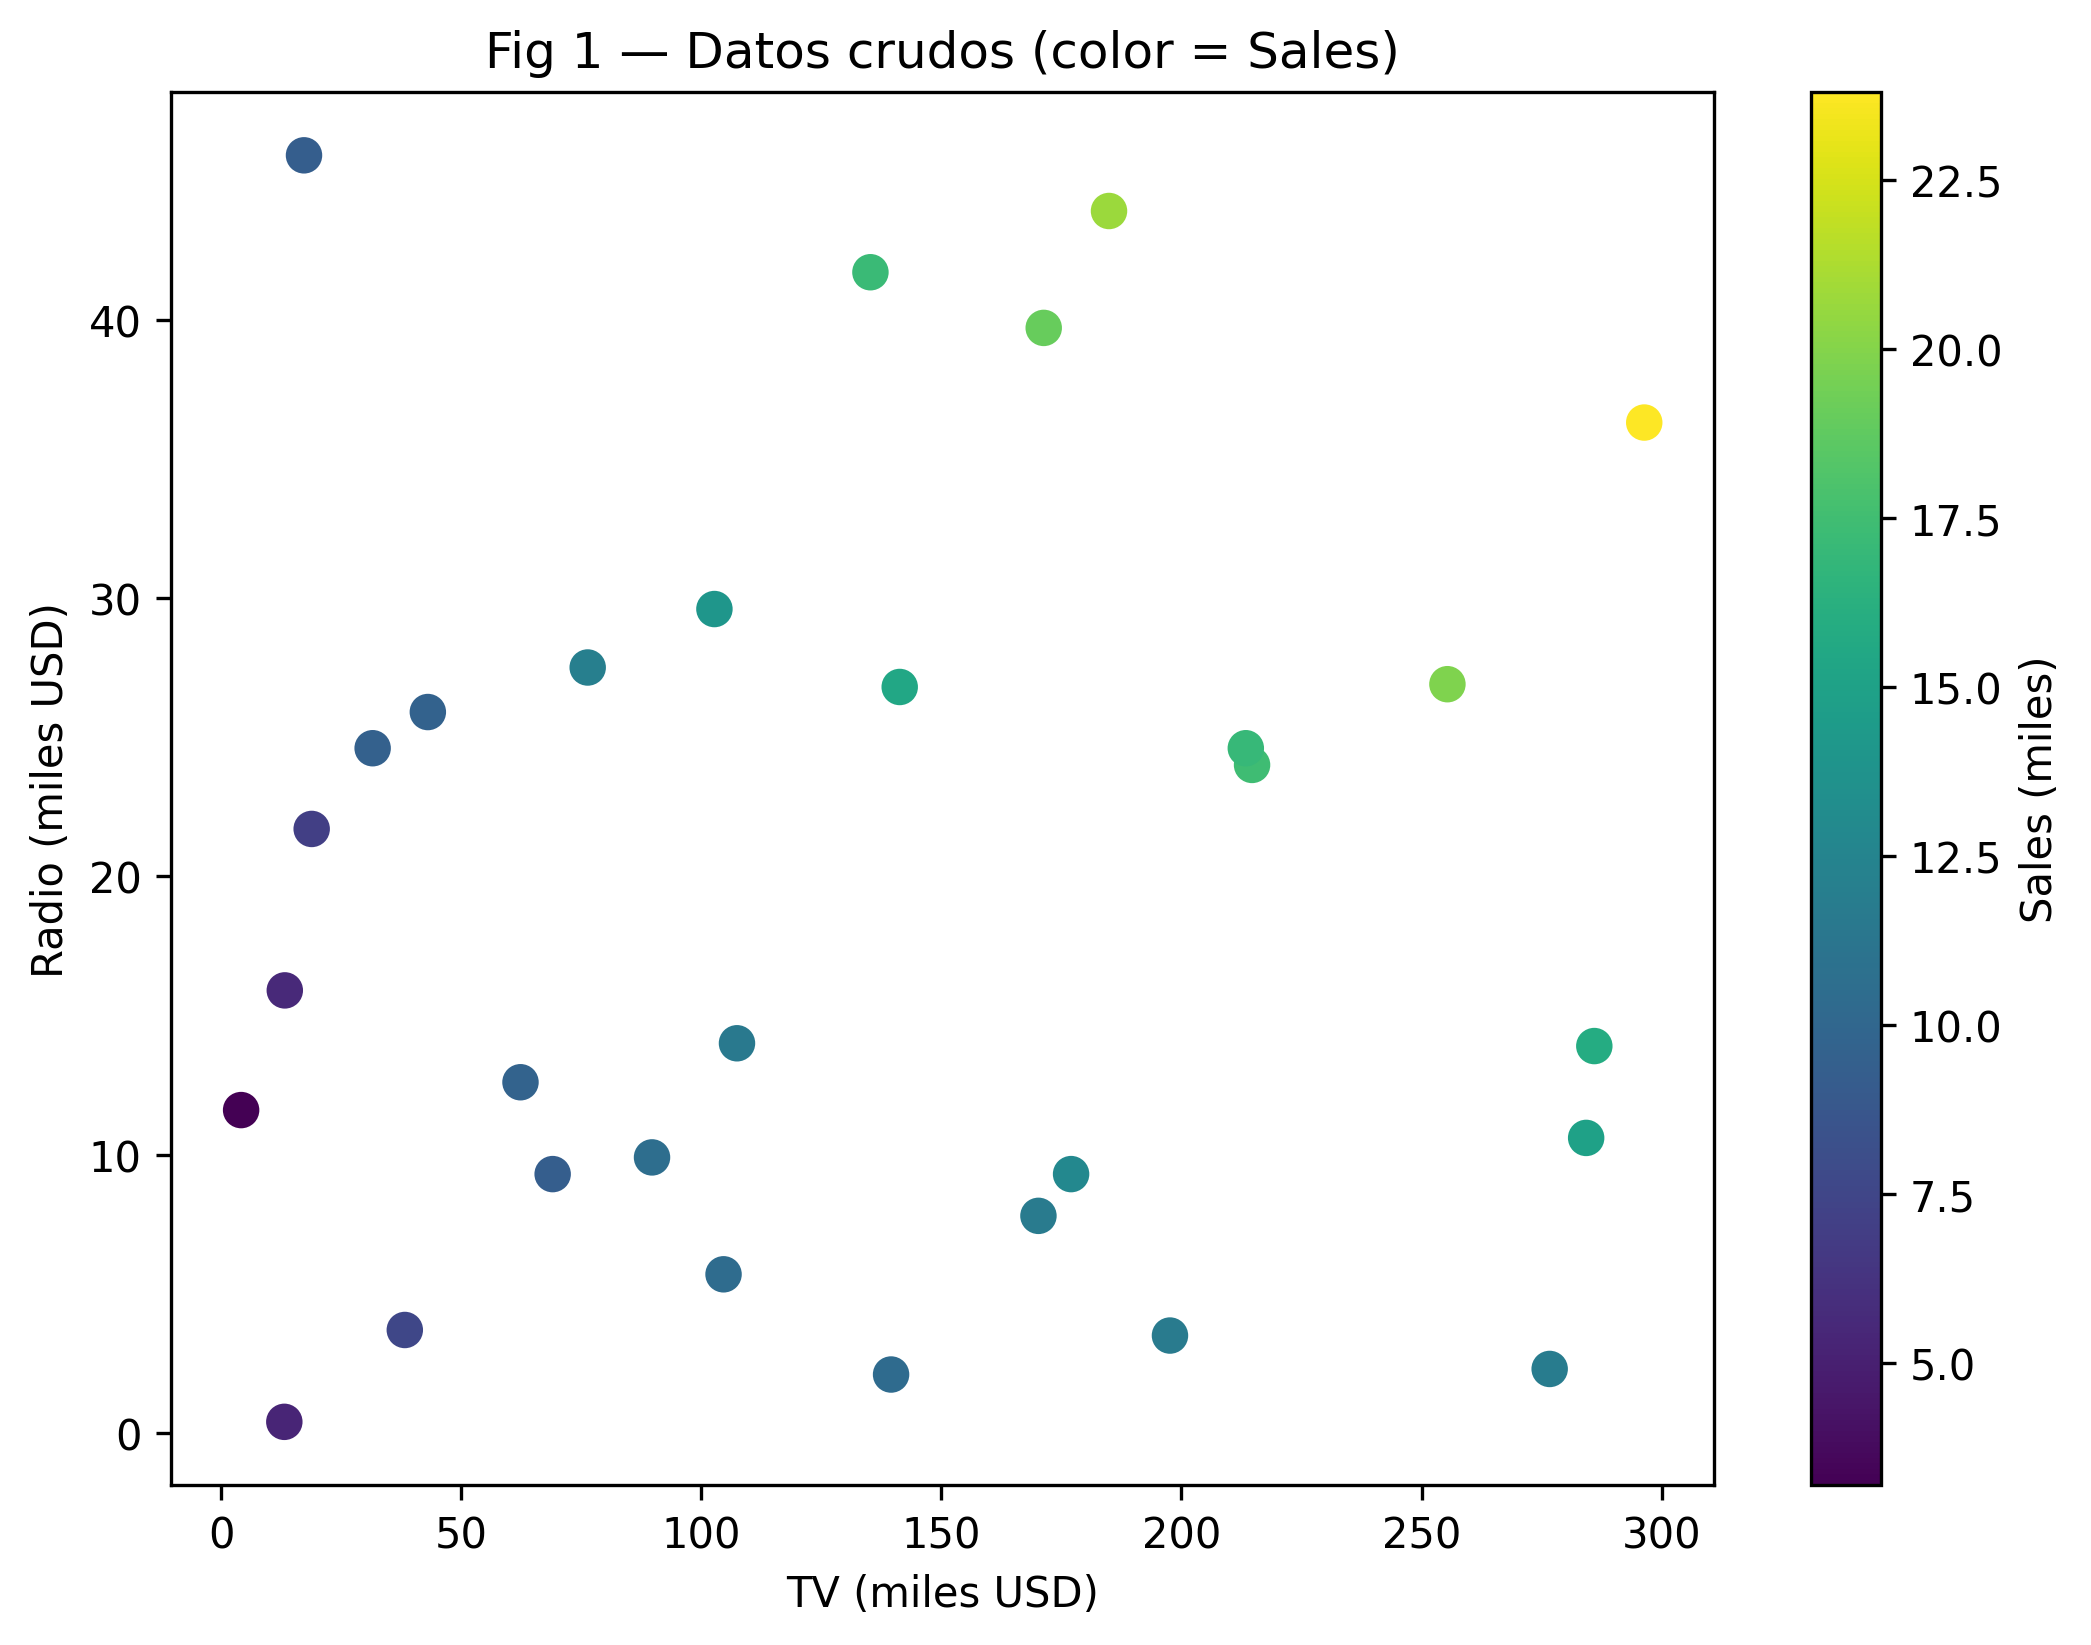
\includegraphics[width=0.75\textwidth]{04_marco_teorico/images/fig1_datos_crudos.png}
\caption{Distribución original de los datos en el plano TV--Radio.}
\label{fig:datos_crudos}
\end{figure}

El primer paso del algoritmo consiste en elegir el corte que maximiza la
reducción de impureza. La Figura~\ref{fig:split1} muestra el primer split
seleccionado en el nodo raíz.

\begin{figure}[H]
\centering
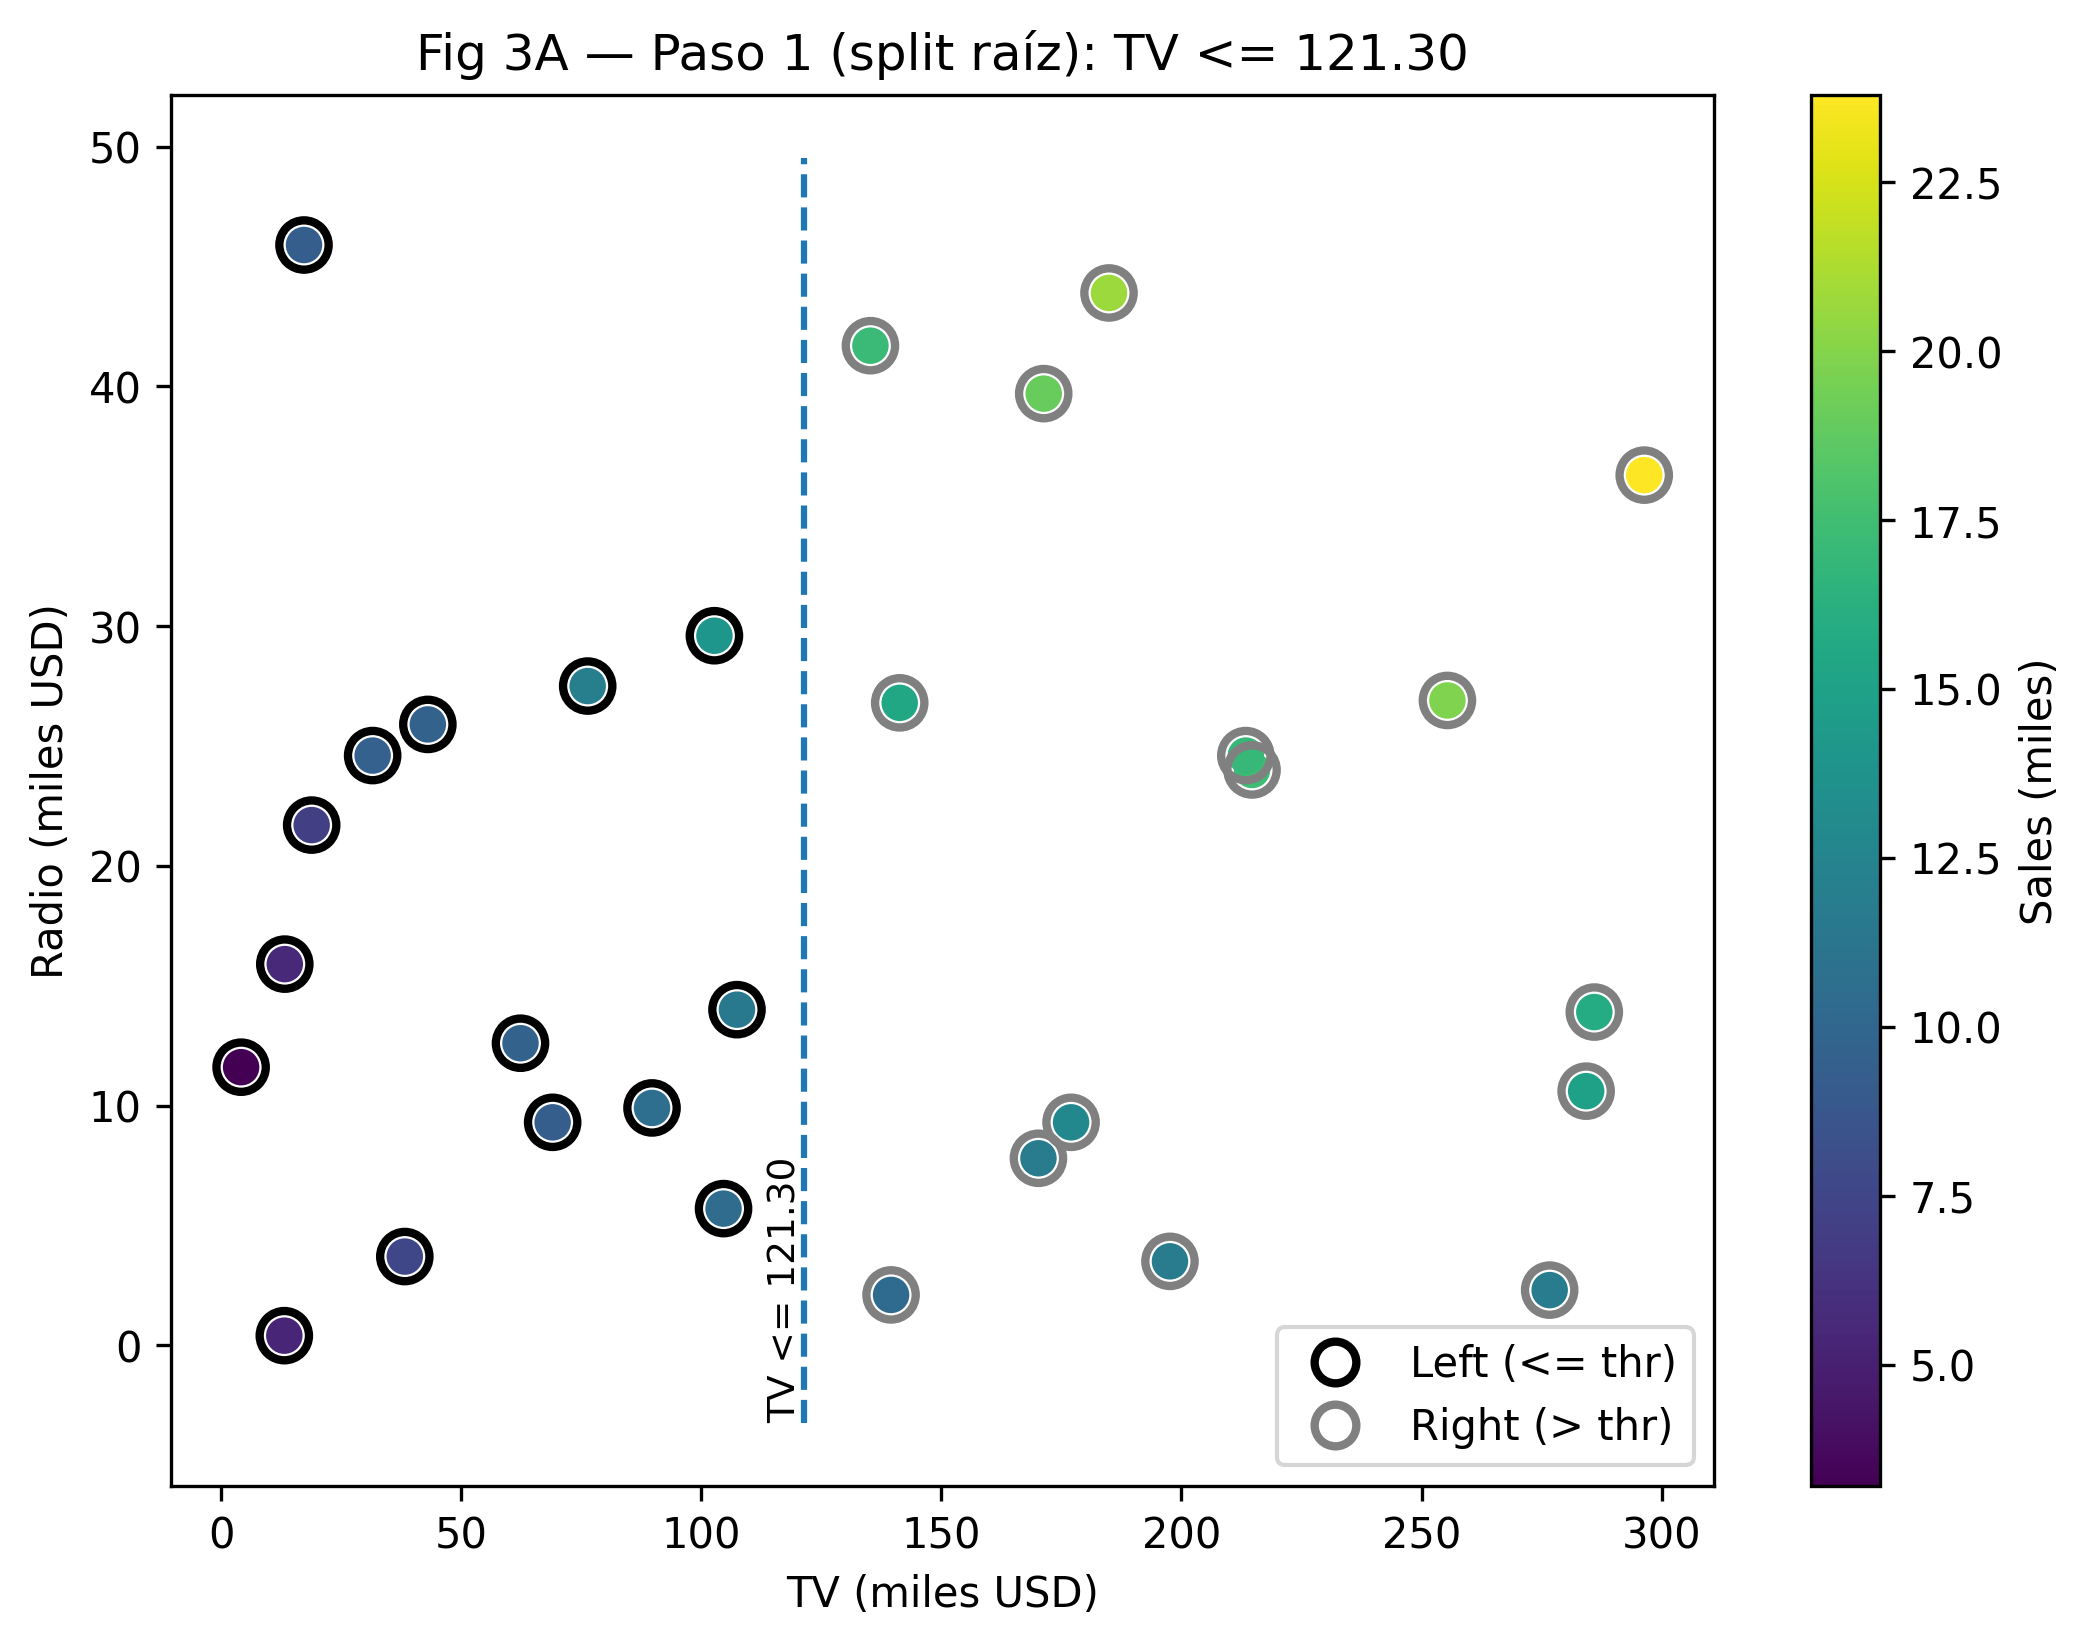
\includegraphics[width=0.75\textwidth]{04_marco_teorico/images/fig3A_paso1_split_raiz.png}
\caption{Primer split seleccionado por el árbol.}
\label{fig:split1}
\end{figure}

En este caso, el algoritmo selecciona una división sobre la variable TV,
con un umbral aproximado de 121.3. Esta recta vertical separa el conjunto de
datos en dos regiones: a la izquierda, observaciones con menor inversión en
televisión, y a la derecha, aquellas con mayor inversión. La elección de este
corte se debe a que produce la mayor reducción de la varianza de la variable
objetivo (Sales) entre todas las divisiones candidatas evaluadas.

La Figura~\ref{fig:tabla_root} muestra la comparación cuantitativa entre este
corte y una alternativa posible.

\begin{figure}[H]
\centering
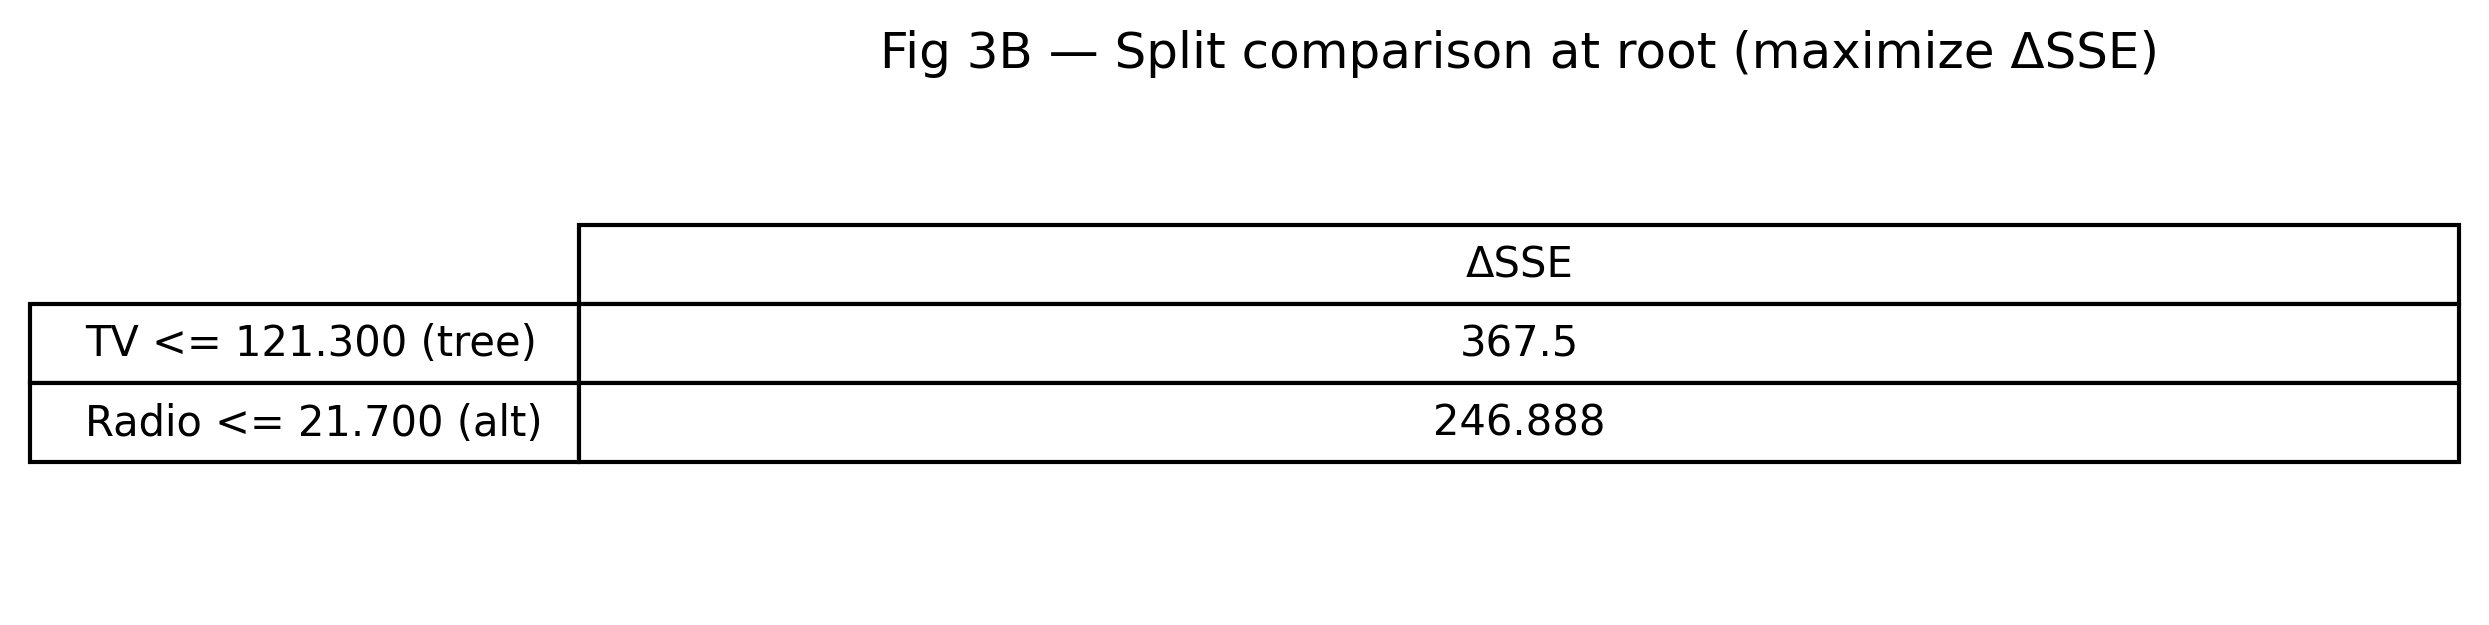
\includegraphics[width=0.9\textwidth]{04_marco_teorico/images/fig3B_tabla_root_vs_alt.png}
\caption{Comparación entre splits en el nodo raíz.}
\label{fig:tabla_root}
\end{figure}

El procedimiento se repite recursivamente. En la Figura~\ref{fig:split23} se
muestran el segundo y tercer corte acumulados, que continúan refinando las
regiones definidas previamente.

\begin{figure}[H]
\centering
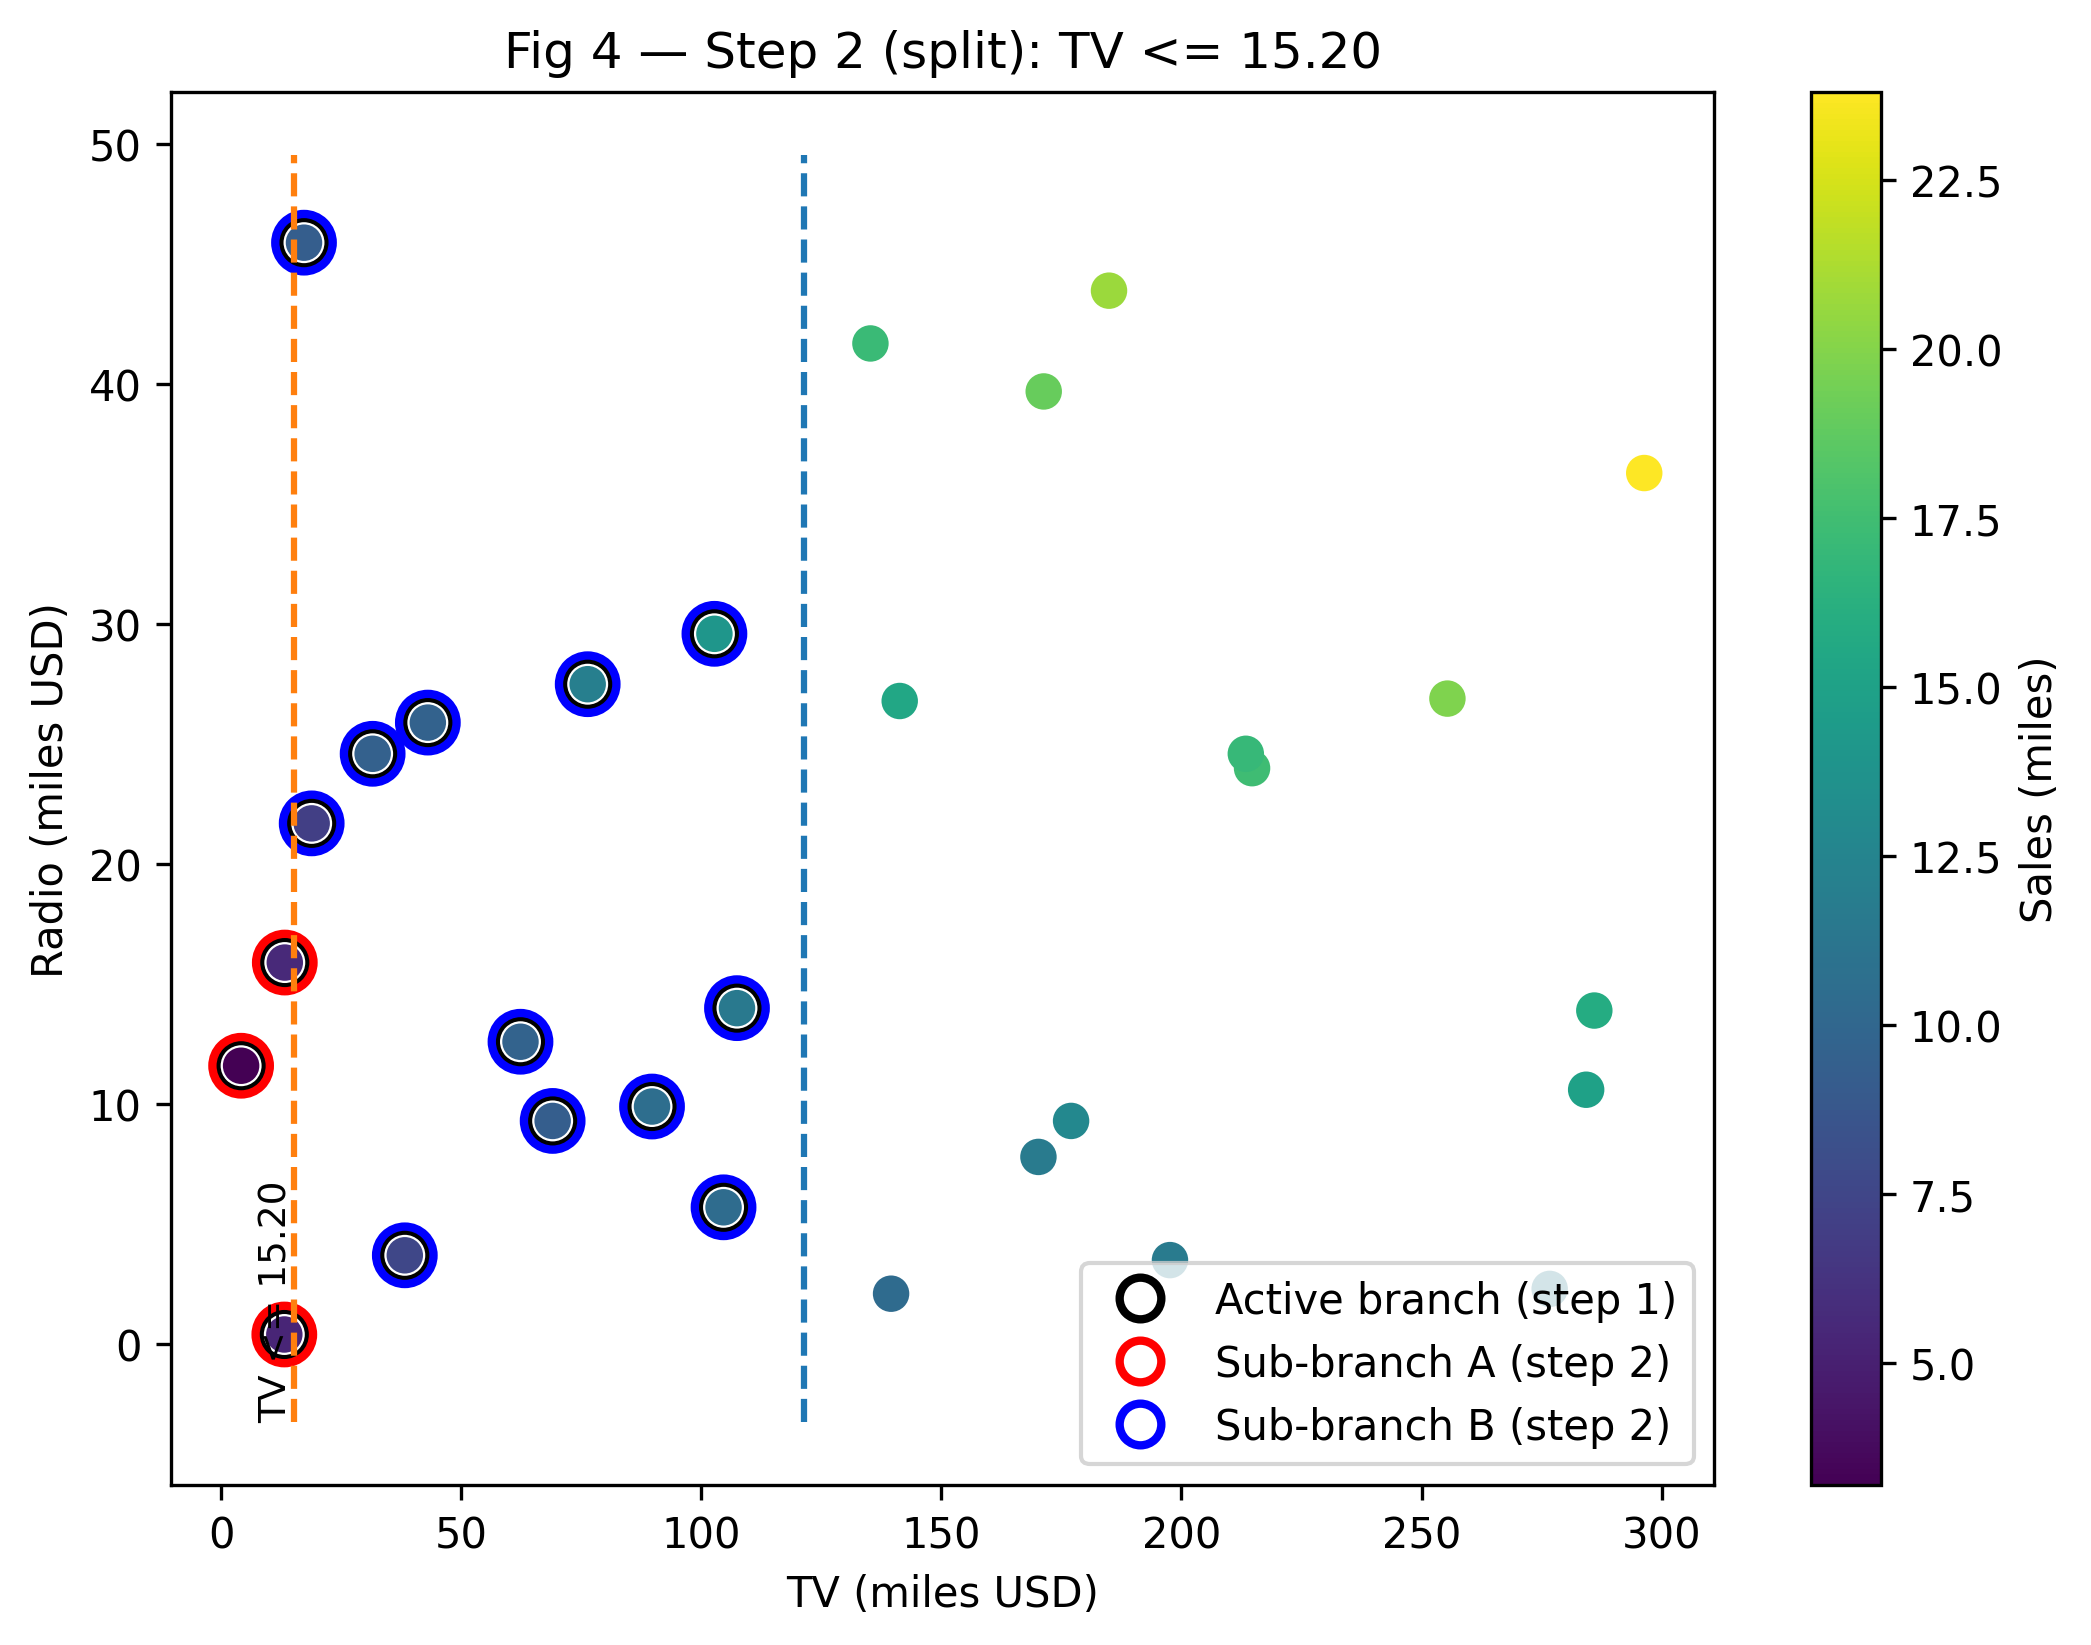
\includegraphics[width=0.5\textwidth]{04_marco_teorico/images/fig4_paso2_split_acumulado.png}\hfill
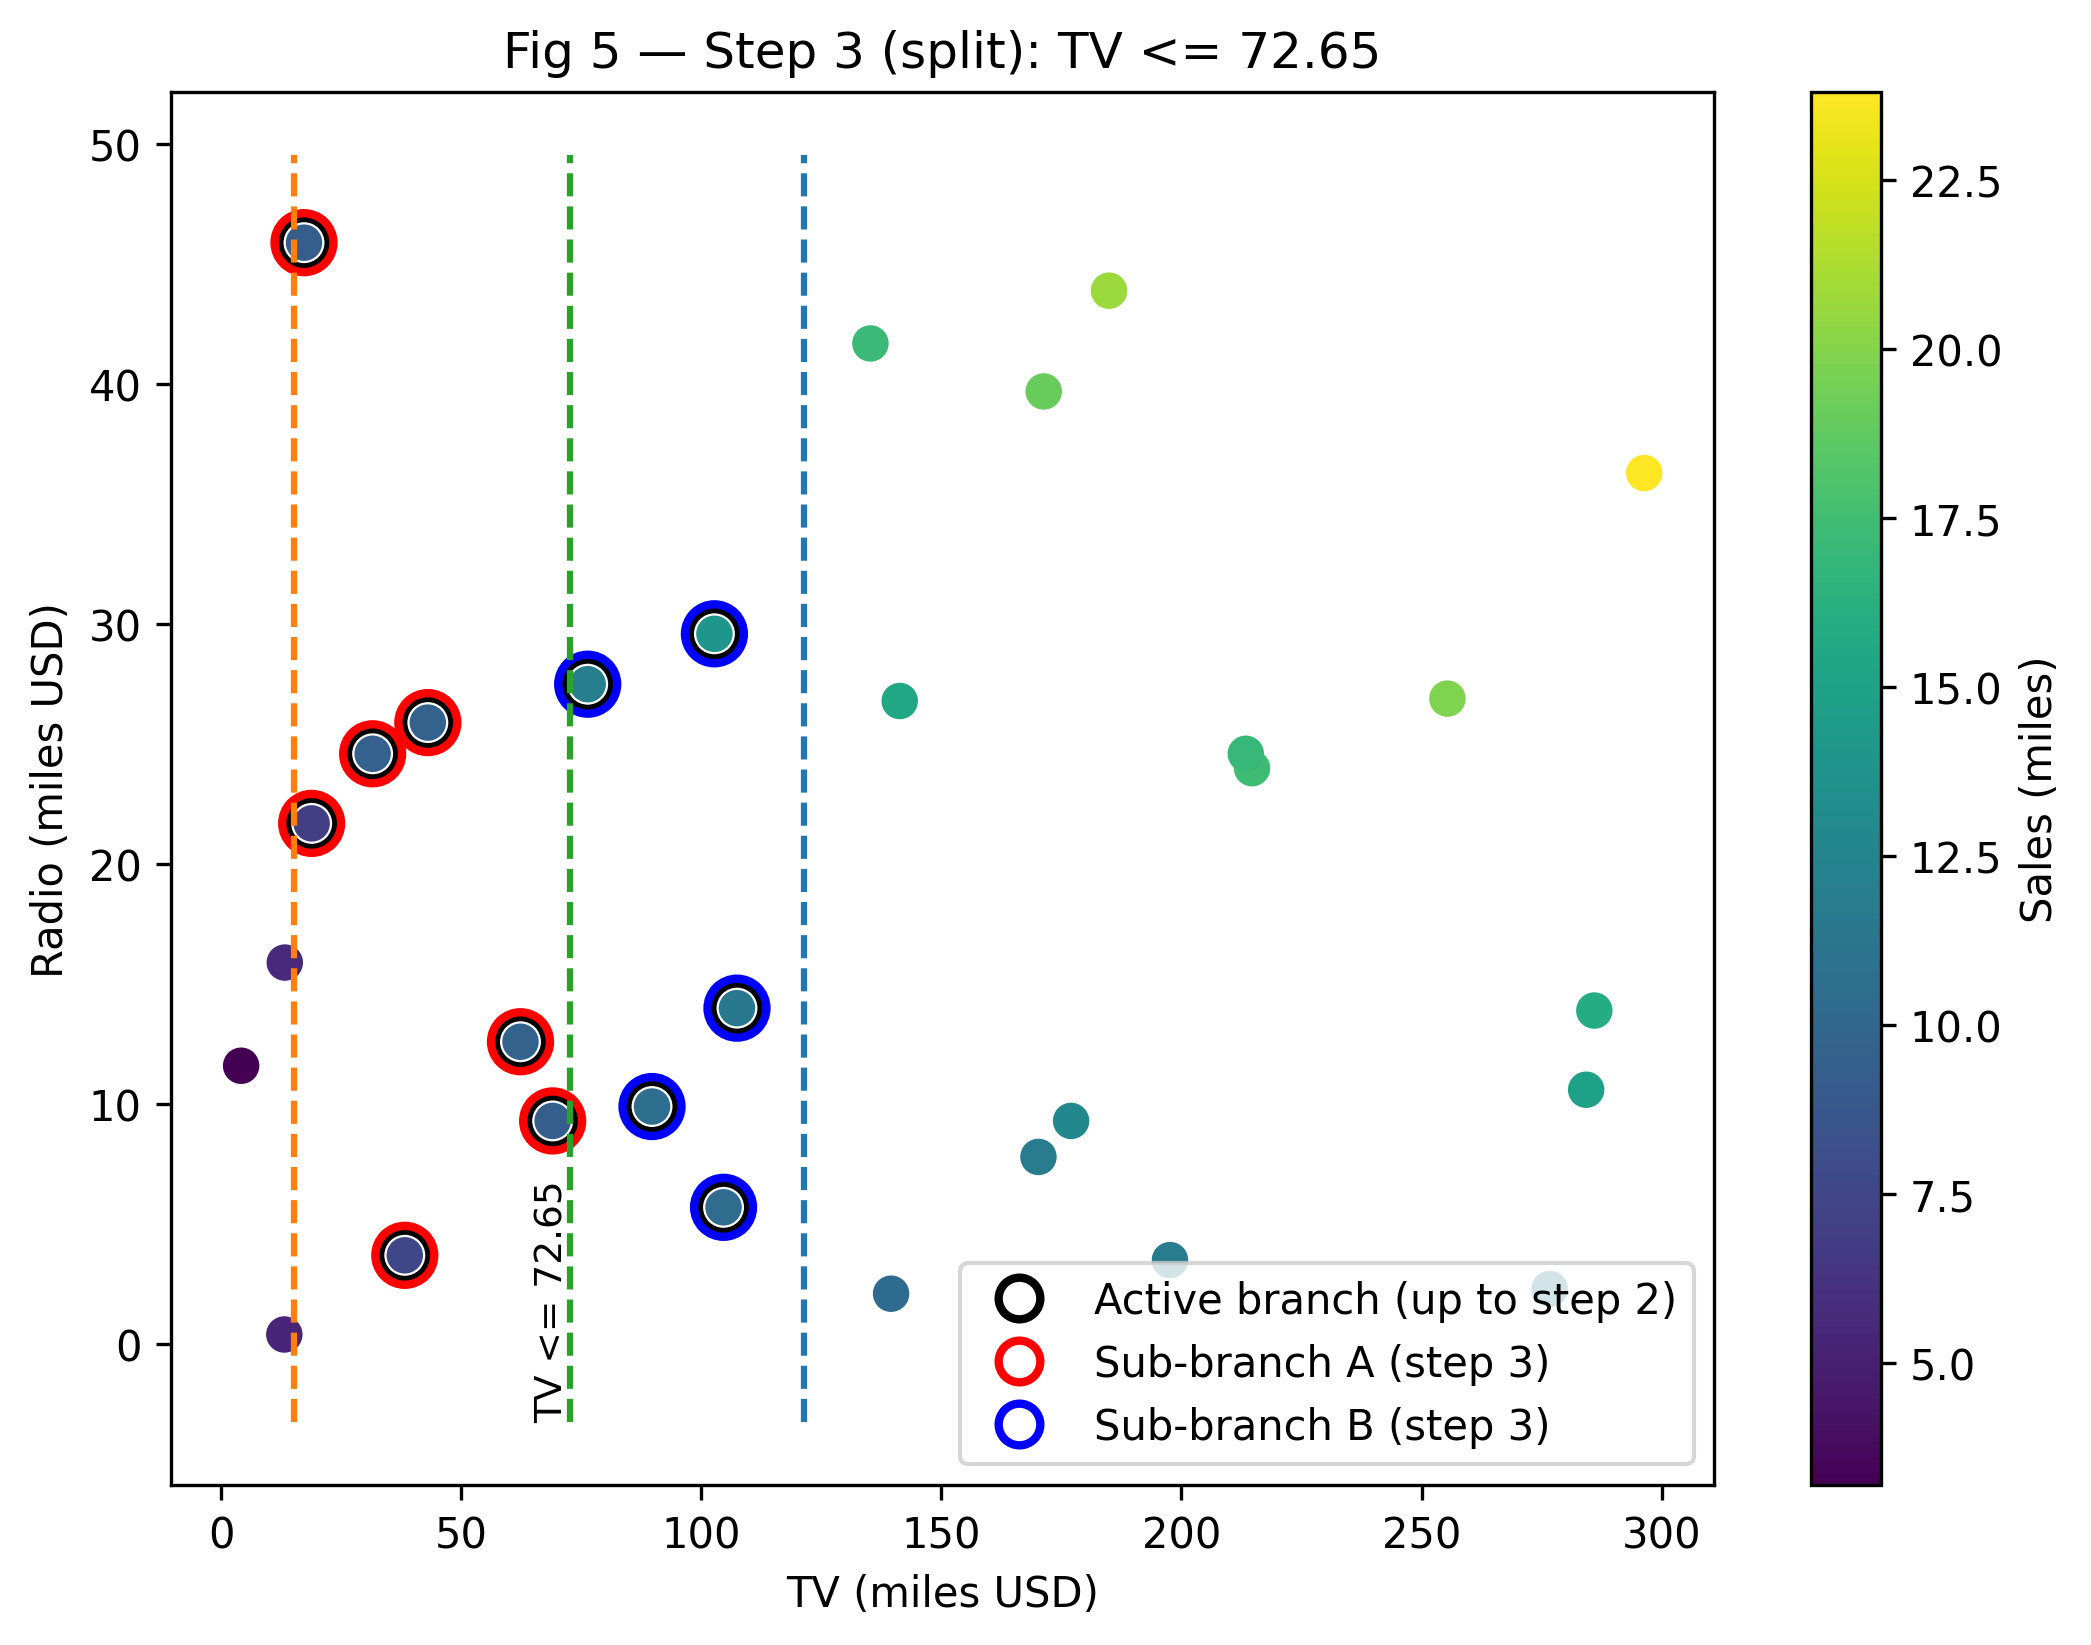
\includegraphics[width=0.5\textwidth]{04_marco_teorico/images/fig5_paso3_split_acumulado.png}
\caption{Segundo y tercer split acumulados.}
\label{fig:split23}
\end{figure}

En este nivel, los nuevos cortes ya no se aplican sobre todo el conjunto de
datos, sino únicamente sobre la región activa heredada del nodo anterior.
De este modo, cada split refina una subregión específica del espacio,
generando particiones cada vez más pequeñas y especializadas.

El resultado final de este proceso es una partición en regiones rectangulares,
donde cada región recibe una predicción constante
(Figura~\ref{fig:regiones}).

\begin{figure}[H]
\centering
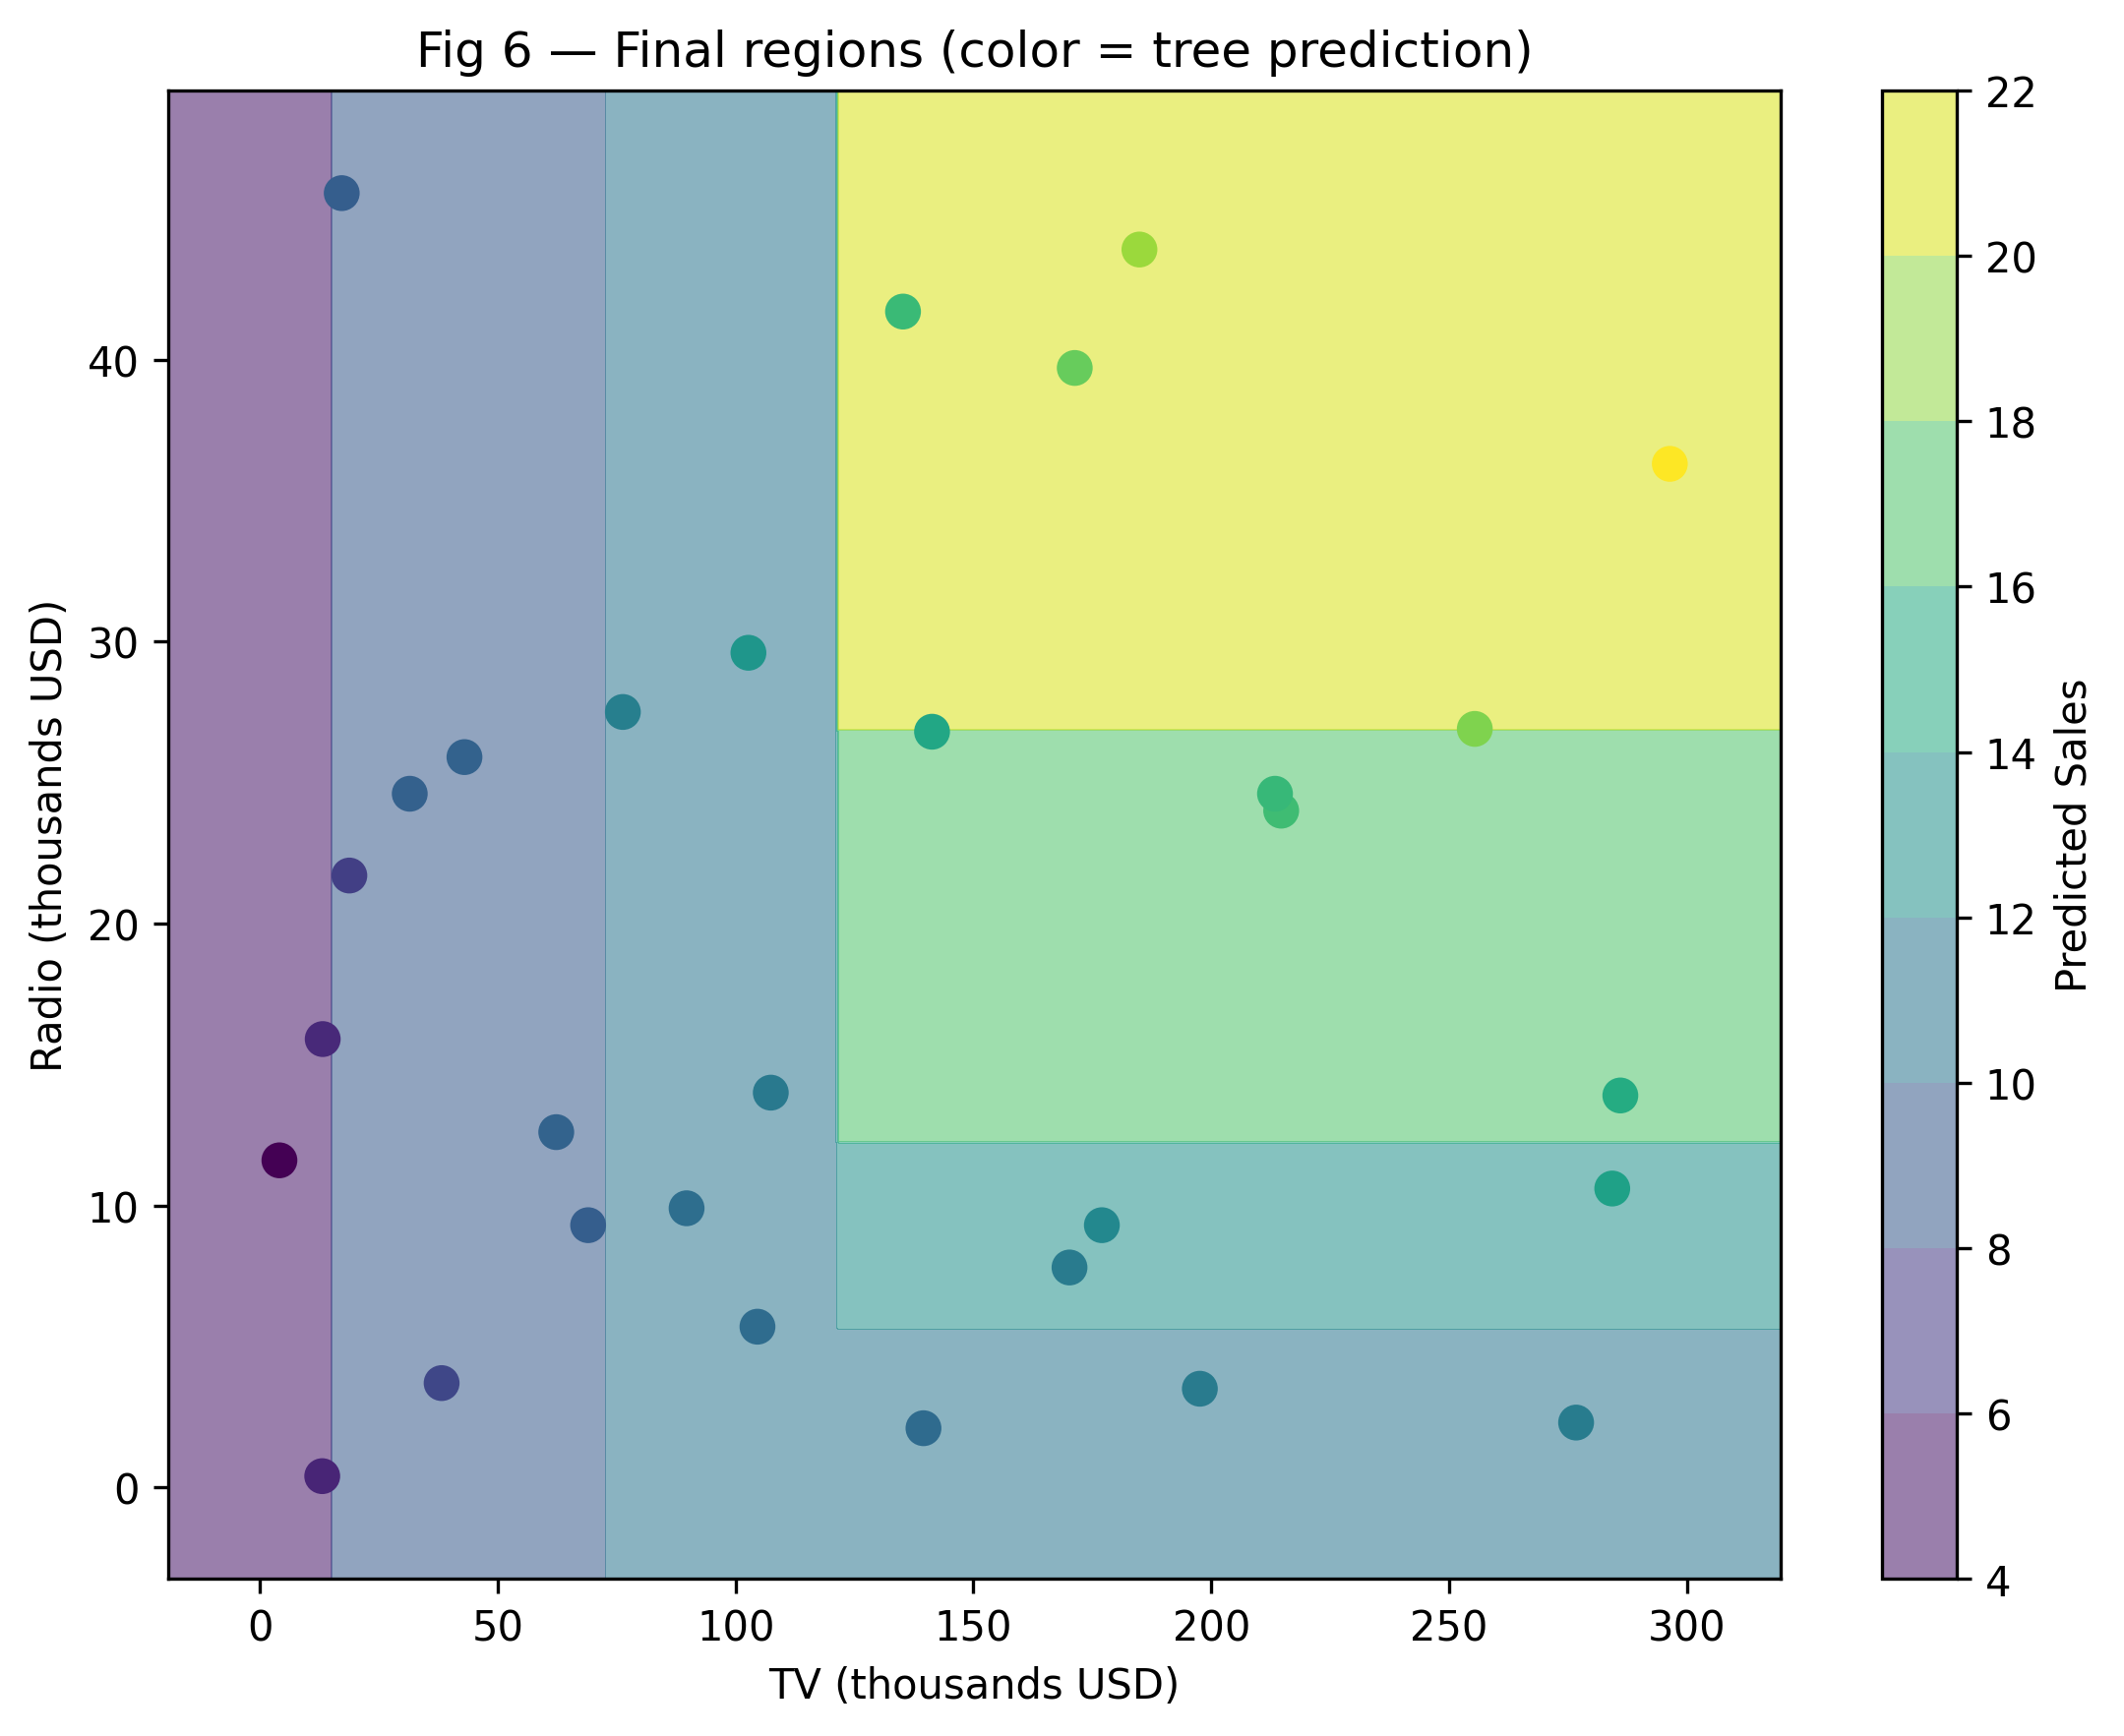
\includegraphics[width=0.75\textwidth]{04_marco_teorico/images/fig6_regiones_finales.png}
\caption{Regiones finales inducidas por el árbol.}
\label{fig:regiones}
\end{figure}

Cada rectángulo coloreado corresponde a una hoja del árbol y representa una
región del espacio de entrada en la que la predicción es constante. El color
indica el valor de predicción (promedio de la variable objetivo) asignado por
el árbol en esa región, de modo que dos puntos ubicados dentro del mismo
rectángulo reciben exactamente la misma salida, independientemente de su
posición específica.

Finalmente, la Figura~\ref{fig:punto} ilustra el recorrido de una observación
nueva hasta una de las hojas, mostrando cómo se obtiene su predicción al
ubicarla en la región correspondiente.

\begin{figure}[H]
\centering
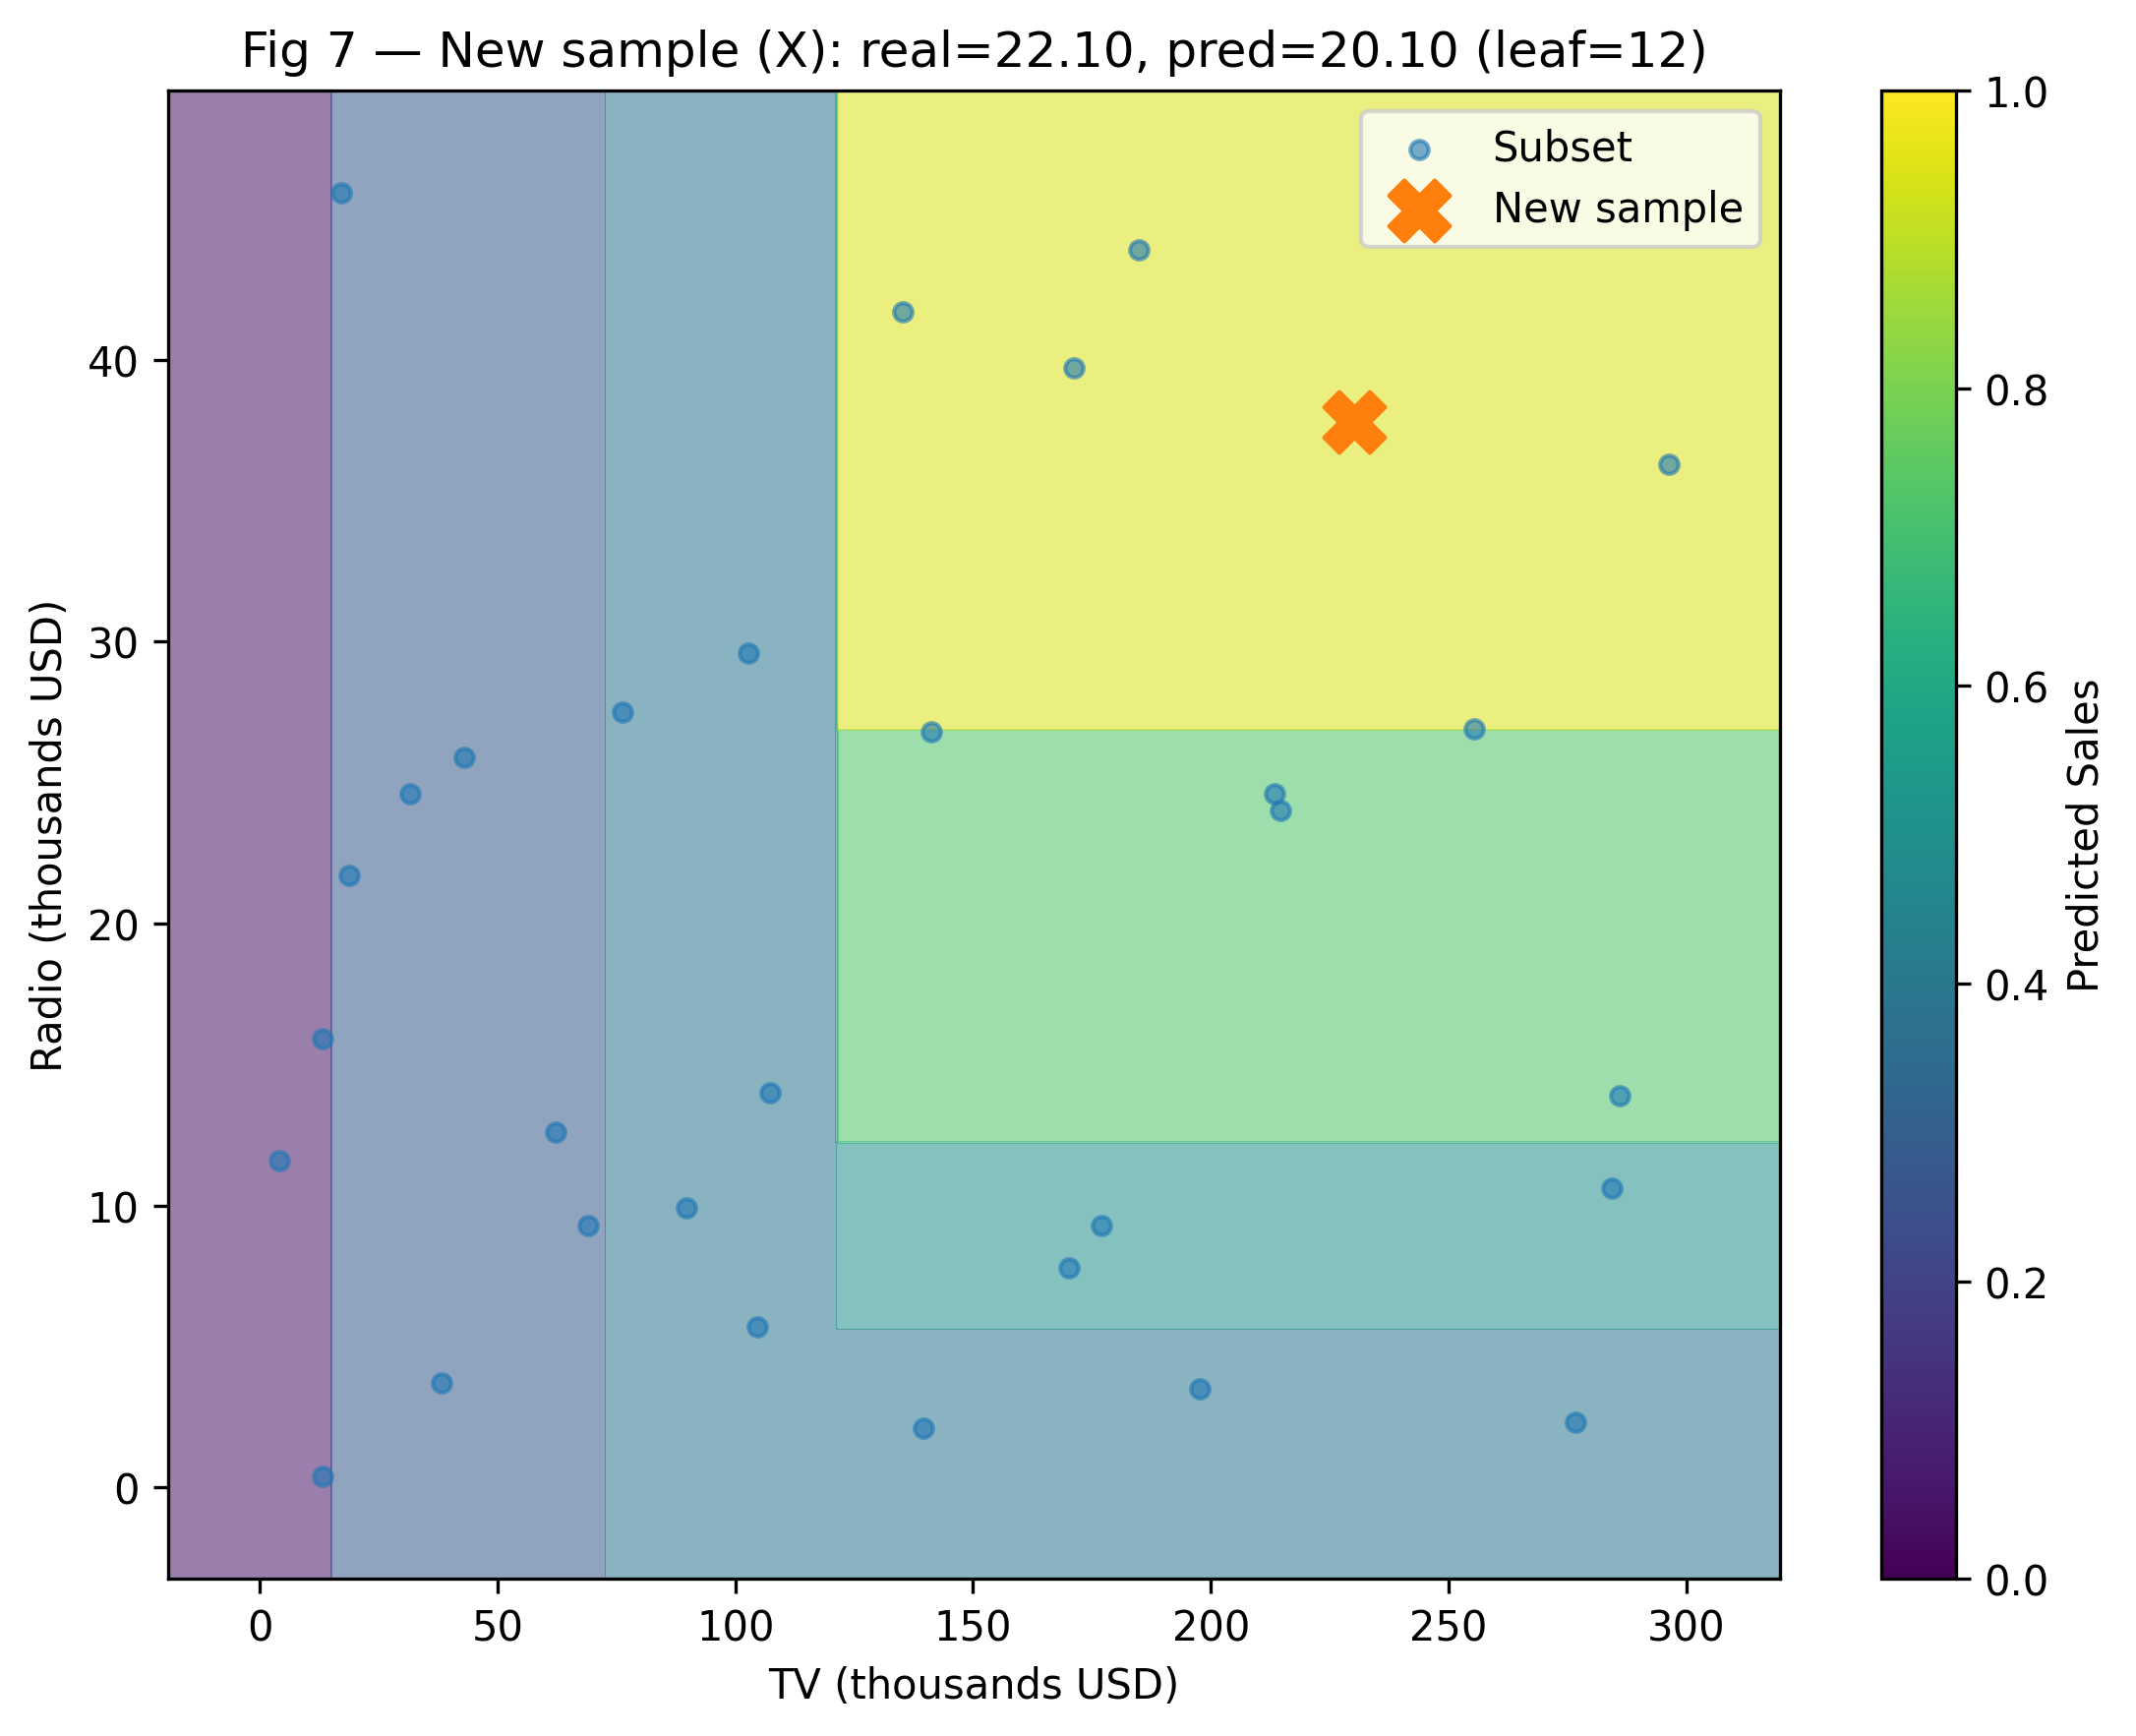
\includegraphics[width=0.75\textwidth]{04_marco_teorico/images/fig7_punto_nuevo_real_vs_pred.png}
\caption{Predicción de un nuevo punto.}
\label{fig:punto}
\end{figure}

Este recorrido resume cómo una partición del espacio de entrada induce una
regla de decisión para cualquier nueva observación. En particular, la región
en la que cae el punto está asociada a una hoja específica del árbol, donde se
almacena el valor de predicción asignado. En el ejemplo mostrado, el modelo
predice $20.1$ frente a un valor real de $22.1$ (error absoluto $=2.0$).

El conjunto completo de reglas generadas por los splits sucesivos queda
codificado en el árbol aprendido, que se muestra en la
Figura~\ref{fig:arbol_completo}.

\begin{figure}[H]
\centering
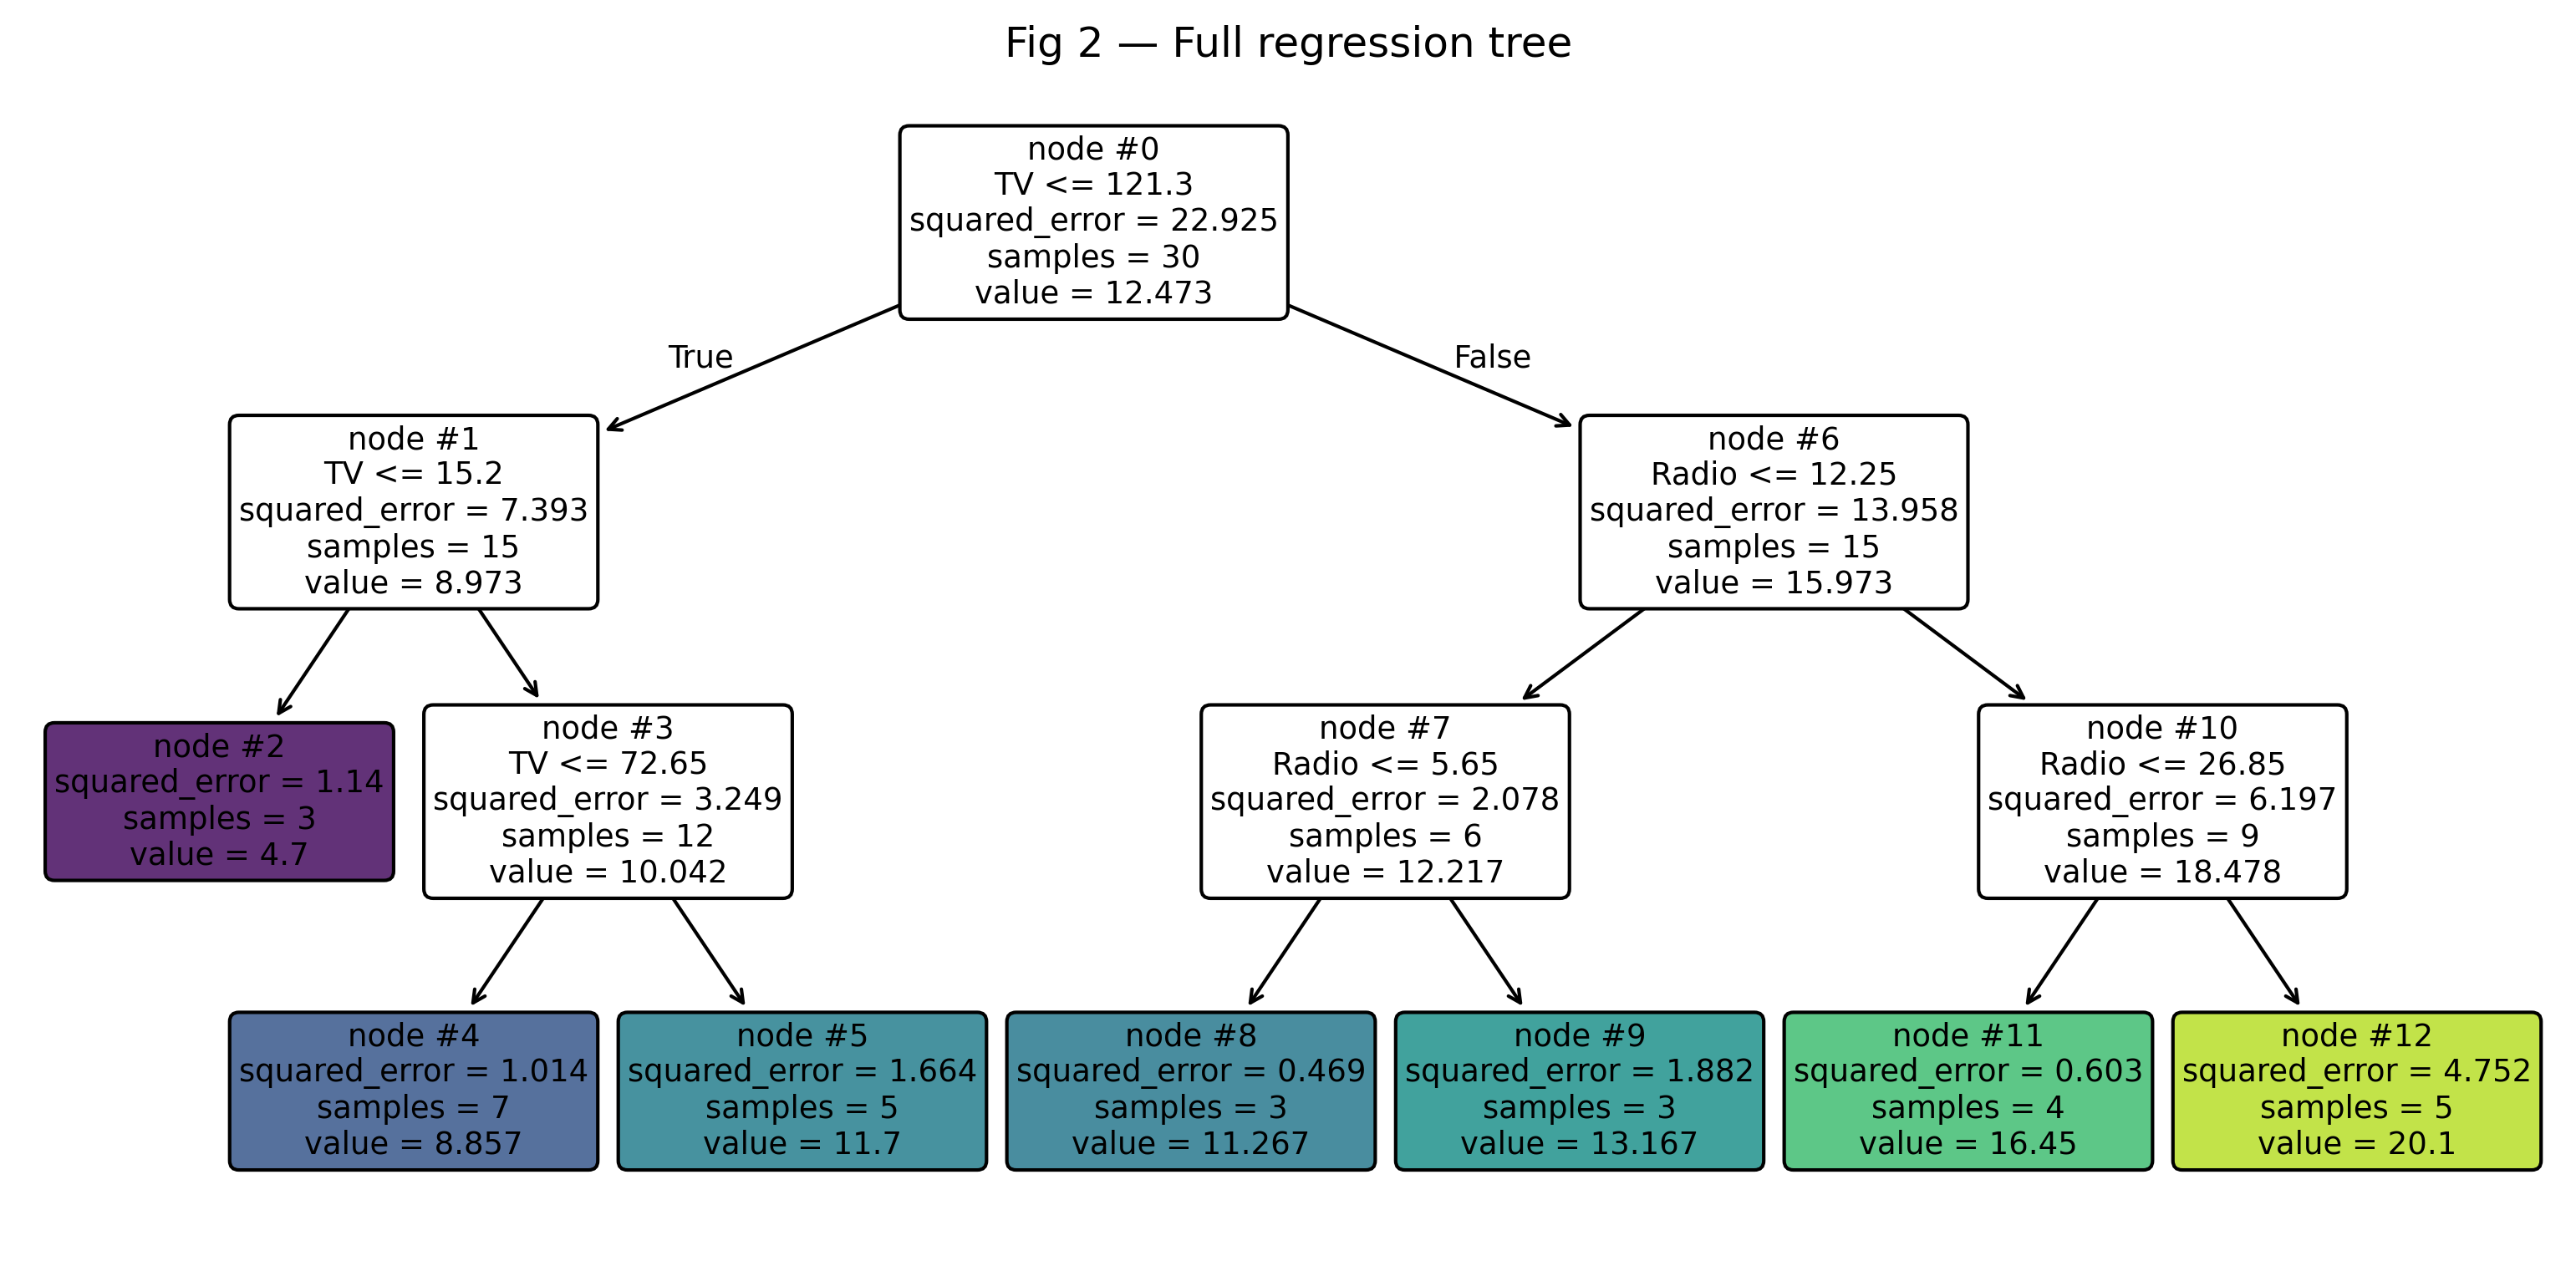
\includegraphics[width=0.99\textwidth]{04_marco_teorico/images/fig2_arbol_completo.png}
\caption{Árbol de regresión completo.}
\label{fig:arbol_completo}
\end{figure}

La estructura del árbol permite visualizar de forma explícita todas las
divisiones aprendidas por el modelo, así como los valores de predicción
asignados en cada hoja.

\medskip

Entre las principales ventajas de los árboles de regresión se encuentra su
capacidad para modelar relaciones no lineales y su interpretación intuitiva.
Sin embargo, presentan una alta tendencia al sobreajuste, ya que pueden
adaptarse excesivamente a los datos de entrenamiento si no se controlan
mediante criterios de parada o regularización. Además, pequeñas variaciones
en los datos pueden producir árboles muy diferentes
\cite{loh2011classification}.

Estas limitaciones motivan el uso de métodos basados en \textit{ensambles},
como el boosting, donde múltiples árboles se combinan para obtener modelos
más robustos, como se describe en la siguiente sección.

\subsubsection{Modelos de ensamble}

Los modelos de \textit{ensamble} combinan múltiples modelos base con el objetivo de obtener un predictor más robusto y preciso que cualquiera de ellos por separado. La idea central es que distintos modelos pueden capturar diferentes aspectos de los datos y que su combinación permite reducir errores y mejorar la capacidad de generalización.

Dentro de este enfoque, existen dos grandes familias: \textit{bagging} y \textit{boosting}, que difieren fundamentalmente en la forma en que se construyen y combinan los modelos.

\paragraph{Bagging.}

Bagging (\textit{Bootstrap Aggregating}) se basa en el muestreo repetido del conjunto de entrenamiento mediante técnicas de \textit{bootstrap}. Dado un conjunto original de $n$ observaciones, se construyen múltiples subconjuntos del mismo tamaño $n$ muestreando con reemplazo. Cada uno de estos subconjuntos contiene los mismos datos originales, pero con repeticiones y omisiones aleatorias.

Sobre cada uno de estos subconjuntos se entrena un modelo independiente, típicamente un árbol de decisión. Este procedimiento se repite muchas veces, generando un conjunto de modelos que, si bien comparten la misma distribución subyacente, presentan diferencias debido al muestreo. La predicción final se obtiene combinando las predicciones individuales, usualmente mediante el promedio en problemas de regresión o el voto mayoritario en clasificación. De este modo, bagging reduce la varianza del modelo y lo hace más estable frente a pequeñas perturbaciones en los datos \cite{breiman1996bagging, hastie2009elements}.
\paragraph{Boosting.}
Boosting sigue una filosofía distinta. En lugar de entrenar modelos independientes, construye una secuencia de modelos de manera iterativa, donde cada nuevo modelo se entrena con el objetivo explícito de corregir los errores cometidos por los anteriores. El procedimiento comienza entrenando un primer modelo sobre el conjunto de datos original. A partir de sus errores, se modifica la distribución de los datos para dar mayor énfasis a las observaciones peor predichas. Con esta versión reponderada del conjunto de entrenamiento se ajusta un nuevo modelo, que intenta corregir las deficiencias del anterior. Este proceso se repite sucesivamente, generando una secuencia de modelos cada vez más especializados en los casos difíciles \cite{schapire1990strength}.

\paragraph{Boosting y teoría PAC.}
Cada uno de los modelos utilizados en boosting es un \textit{weak learner}, es decir, un modelo cuya capacidad predictiva es apenas mejor que la de una predicción aleatoria \cite{kearns1994cryptographic}. En el marco de la teoría PAC (\textit{Probably Approximately Correct}), un algoritmo se considera un weak learner si logra, con alta probabilidad, un error ligeramente menor que el de una elección al azar \cite{valiant1984theory}. A pesar de su debilidad individual, la combinación secuencial de estos modelos permite construir un predictor final considerablemente más potente.

Desde un punto de vista teórico, se demostró que las nociones de
\textit{strong learnability} y \textit{weak learnability} son equivalentes,
es decir, que si una clase de problemas puede ser aprendida por un modelo
fuerte, entonces también puede ser aprendida combinando modelos débiles.
Este resultado fue formalizado por Schapire \cite{schapire1990strength},
resolviendo el denominado \textit{hypothesis boosting problem}.

En este contexto, una \textit{hipótesis} representa el modelo aprendido en
cada iteración, es decir, la función que asigna una predicción a partir de
las variables de entrada.

Una de las primeras construcciones que materializan este resultado fue el
denominado \textit{hypothesis boosting mechanism}, propuesto como una
demostración conceptual de cómo combinar hipótesis débiles para obtener un
clasificador fuerte. En este esquema, se construyen varias hipótesis a partir
de subconjuntos de datos seleccionados de manera adaptativa, es decir,
construidos en función de los errores cometidos por las hipótesis anteriores.
Las predicciones se combinan y se refuerzan aquellas que corrigen los errores
de las anteriores. Si bien este enfoque no fue concebido como un algoritmo
práctico escalable, sentó las bases conceptuales para los métodos modernos de
boosting.

\paragraph{AdaBoost.}
A partir de estas ideas surge \textit{AdaBoost} (Adaptive Boosting), una de las variantes más influyentes de boosting. En AdaBoost, cada muestra del conjunto de entrenamiento posee un peso que se actualiza iterativamente. Al inicio, todas las observaciones tienen la misma importancia. Luego de entrenar un modelo, se incrementan los pesos de las observaciones mal clasificadas y se reducen los de aquellas correctamente clasificadas, de modo que el siguiente modelo se concentre en los ejemplos más difíciles \cite{freund1997decision, freund1999short}. Además, cada modelo entrenado recibe una importancia relativa en la combinación final, de acuerdo con su desempeño.

Si no se utilizan suficientes iteraciones, el modelo resultante puede ser demasiado simple y presentar subajuste. Sin embargo, cuando se emplean modelos base débiles, como árboles de decisión poco profundos, boosting tiende a ser relativamente robusto frente al sobreajuste. 

No obstante, AdaBoost presenta limitaciones importantes en problemas de regresión y en escenarios con ruido o valores atípicos, ya que está estrechamente ligado a una función de pérdida exponencial fija. Esta falta de flexibilidad dificulta su adaptación a tareas donde se requieren otras funciones de error, como la predicción de variables continuas complejas.

\paragraph{Gradient Boosting.}
Otra variante ampliamente utilizada es \textit{Gradient Boosting}, que reformula el
proceso de boosting desde una perspectiva de optimización. En lugar de modificar
explícitamente los pesos de las observaciones, este enfoque utiliza los gradientes
de una función de pérdida para identificar qué ejemplos están siendo peor predichos.

En cada iteración, el nuevo modelo se entrena para aproximar el
\textit{gradiente negativo} de dicha función de pérdida, de modo que el ensamble
completo avanza en la dirección que reduce el error global. Desde este punto de
vista, el proceso puede interpretarse como una optimización por etapas
\cite{friedman2001greedy,natekin2013gradient}.

Una ventaja fundamental de este enfoque es que permite utilizar funciones de
pérdida arbitrarias. Por ejemplo, si se emplea el error cuadrático medio, el
procedimiento equivale a ajustar modelos sucesivos a los errores residuales del
modelo actual \cite{friedman2001greedy,natekin2013gradient}.


Mientras que en AdaBoost las dificultades se reflejan en pesos elevados asignados
a ciertas observaciones, en Gradient Boosting se manifiestan como gradientes de
mayor magnitud.

Sobre esta base, se utilizan variantes modernas de boosting para mejorar
el rendimiento y el control del sobreajuste, entre ellas XGBoost, que será
el modelo supervisado principal en este trabajo y se describe a continuación.

\subsubsection{XGBoost}

La descripción presentada en esta sección se basa principalmente en el trabajo
de Chen y Guestrin \cite{chen2016xgboost}, quienes introducen XGBoost como un sistema de
\textit{gradient tree boosting} orientado a combinar alto rendimiento
predictivo con escalabilidad computacional.

XGBoost (eXtreme Gradient Boosting) es un sistema de aprendizaje supervisado
basado en \textit{Gradient Boosting} con árboles de decisión, diseñado para
ofrecer alto rendimiento predictivo y, al mismo tiempo, escalar de manera
eficiente a grandes volúmenes de datos.  

Desde el punto de vista conceptual, XGBoost sigue el mismo principio que
Gradient Boosting: construir un modelo aditivo que combina múltiples árboles
de decisión entrenados de forma secuencial, donde cada nuevo árbol se ajusta
para corregir los errores cometidos por el ensamble actual. En el contexto de
regresión, esto equivale a aproximar progresivamente la función objetivo
mediante pequeños ajustes que reducen el error global.

La principal diferencia con implementaciones tradicionales de Gradient
Boosting es que XGBoost incorpora, de manera explícita, mecanismos de
regularización y una serie de optimizaciones algorítmicas y computacionales
que permiten entrenar modelos más estables y eficientes, especialmente en
escenarios de alta dimensionalidad.

\paragraph{Función objetivo regularizada.}
XGBoost define una función objetivo que combina dos términos:  
(i) una función de pérdida que mide el error entre las predicciones y los
valores reales, y  
(ii) un término de regularización que penaliza la complejidad de los árboles.
  
Este segundo término controla el número de hojas y la magnitud de los valores
predichos en cada nodo, evitando que el modelo se adapte en exceso a los datos
de entrenamiento. De esta forma, XGBoost logra un mejor equilibrio entre
capacidad de ajuste y generalización.

\paragraph{Árboles ajustados a los residuos.}
El entrenamiento comienza con una predicción inicial constante. A partir de
ella, se calculan los errores (o residuos) entre las predicciones actuales y
los valores reales. En cada iteración, se entrena un árbol de regresión que
aproxima estos residuos, y sus predicciones se suman al modelo previo,
escaladas por un factor de aprendizaje.

Por ejemplo, si el modelo subestima sistemáticamente ciertos valores, el
siguiente árbol aprenderá a corregir esa región del espacio de entrada. Este
proceso se repite hasta que el error global deja de disminuir o se alcanza un
número máximo de iteraciones.

\paragraph{Búsqueda eficiente de divisiones.}
Una dificultad central en los árboles de decisión es encontrar, para cada
variable, el punto de corte que mejor separa los datos. En conjuntos grandes,
evaluar todos los valores posibles resulta computacionalmente costoso.

XGBoost utiliza un enfoque aproximado basado en cuantiles: en lugar de probar
todos los cortes posibles, divide cada variable en un conjunto reducido de
intervalos representativos y solo evalúa esos puntos. Para estimar estos
cuantiles sin recorrer todo el conjunto de datos, emplea un algoritmo llamado
\textit{quantile sketch}, que aproxima la distribución de las variables con un
costo computacional muy bajo.

En problemas de clasificación, esta estimación se realiza de forma ponderada,
dando mayor importancia a los ejemplos cuya predicción es más incierta, lo que
permite concentrar el poder del modelo en las regiones más difíciles.

\paragraph{Manejo de datos faltantes y dispersos.}
XGBoost es \textit{sparsity-aware}, es decir, puede manejar valores faltantes de
forma nativa. Cuando una variable contiene valores ausentes, el algoritmo
aprende automáticamente hacia qué rama del árbol debe enviarlos, en función
de qué opción produce menor error. Esta decisión queda almacenada y se aplica
también a nuevos datos.

Este mecanismo resulta especialmente útil en escenarios reales, donde los
datos suelen ser incompletos o dispersos.

\paragraph{Escalabilidad computacional.}
XGBoost fue diseñado para trabajar con grandes volúmenes de datos. Entre sus
principales optimizaciones se incluyen:

\begin{itemize}
  \item Construcción paralela de las divisiones dentro de cada árbol (la evaluación de splits candidatos se distribuye entre múltiples hilos).
  \item Aprendizaje fuera de memoria (\textit{out-of-core}), que permite
  procesar conjuntos de datos que no caben completamente en la memoria RAM.
  \item Acceso eficiente a memoria mediante estructuras de datos que
  priorizan el uso de caché.
  \item Muestreo de observaciones y variables en cada iteración, lo que reduce
  el costo computacional y ayuda a controlar el sobreajuste.
\end{itemize}

\section{Validación, evaluación y optimización de hiperparámetros}
\label{sec:validacion_evaluacion}

\subsection{Partición de datos y validación cruzada}

En problemas de aprendizaje automático, evaluar el rendimiento de un modelo sobre los mismos datos con los que fue entrenado puede llevar a estimaciones excesivamente optimistas del rendimiento real, un fenómeno conocido como sobreajuste. Para obtener una estimación más realista de la capacidad de generalización, los datos se dividen típicamente en al menos dos conjuntos: uno de entrenamiento y uno de test. El modelo se entrena exclusivamente sobre el primero y se evalúa sobre el segundo, que contiene datos no vistos durante el entrenamiento.

Una extensión de esta idea es la \textit{partición holdout} con tres conjuntos: entrenamiento, validación y test. El conjunto de validación se utiliza para la selección de hiperparámetros y decisiones de diseño del modelo, mientras que el conjunto de test se reserva exclusivamente para la evaluación final. Esta separación garantiza que las métricas reportadas no estén sesgadas por las decisiones tomadas durante el desarrollo del modelo.

La \textit{validación cruzada $K$-Fold} es una técnica que permite obtener estimaciones de rendimiento más robustas. Los datos de entrenamiento se dividen en $K$ subconjuntos (folds) de tamaño aproximadamente igual. En cada una de las $K$ iteraciones, uno de los folds se utiliza como conjunto de validación y los $K-1$ restantes como entrenamiento. El rendimiento final se calcula como el promedio de las $K$ evaluaciones. Esta estrategia tiene la ventaja de que cada observación es utilizada exactamente una vez como dato de validación, proporcionando una estimación menos dependiente de una partición particular de los datos \cite{hastie2009elements}.

\subsection{Métricas de regresión}
\label{sec:metricas_regresion}

Para evaluar el rendimiento de modelos de regresión se utilizan diversas métricas que cuantifican la discrepancia entre los valores predichos $\hat{y}_i$ y los valores reales $y_i$. Las métricas más utilizadas incluyen:

\begin{itemize}
    \item \textbf{Error absoluto medio (MAE):}
    \[
    \text{MAE} = \frac{1}{n} \sum_{i=1}^{n} |y_i - \hat{y}_i|.
    \]
    Representa el error promedio en las unidades originales de la variable objetivo (por ejemplo, años). Es interpretable y robusto frente a valores atípicos.

    \item \textbf{Raíz del error cuadrático medio (RMSE):}
    \[
    \text{RMSE} = \sqrt{\frac{1}{n} \sum_{i=1}^{n} (y_i - \hat{y}_i)^2}.
    \]
    Penaliza proporcionalmente más los errores grandes. Siempre se cumple que $\text{RMSE} \geq \text{MAE}$; una diferencia grande entre ambos indica la presencia de errores puntuales de gran magnitud.

    \item \textbf{Coeficiente de determinación ($R^2$):}
    \[
    R^2 = 1 - \frac{\sum_{i=1}^{n} (y_i - \hat{y}_i)^2}{\sum_{i=1}^{n} (y_i - \bar{y})^2},
    \]
    donde $\bar{y}$ es la media de los valores reales. Indica qué proporción de las diferencias individuales en la variable objetivo es capturada por el modelo. Por ejemplo, un $R^2 = 0{,}41$ significa que el modelo explica el 41\% de la variabilidad observada, mientras que el 59\% restante se debe a factores que el modelo no logra capturar. Un valor de $R^2 = 1$ indica predicción perfecta, mientras que $R^2 = 0$ equivale a predecir siempre la media.

    \item \textbf{Correlación de Pearson ($r$):} mide la fuerza de la asociación lineal entre los valores reales y predichos, complementando al $R^2$ con información sobre la dirección y linealidad de la relación.
\end{itemize}

\subsection{Optimización de hiperparámetros}
\label{sec:hpo_theory}

Los modelos de aprendizaje automático dependen de hiperparámetros que no se aprenden durante el entrenamiento sino que se fijan antes de éste, como la tasa de aprendizaje, la dimensión del espacio latente de un autoencoder o la profundidad máxima de un árbol de decisión. La selección de estos hiperparámetros tiene un impacto significativo en el rendimiento del modelo.

Existen diversas estrategias para la búsqueda de hiperparámetros. La búsqueda en grilla (\textit{grid search}) evalúa todas las combinaciones posibles de un conjunto discreto de valores, pero resulta computacionalmente costosa cuando el número de hiperparámetros es grande. La búsqueda aleatoria (\textit{random search}) muestrea configuraciones al azar del espacio de búsqueda, lo que puede ser más eficiente en espacios de alta dimensión.

Los métodos de optimización bayesiana representan un enfoque más sofisticado que modela la relación entre los hiperparámetros y la métrica objetivo mediante un modelo probabilístico. A partir de este modelo, se proponen nuevas configuraciones en regiones del espacio de búsqueda que tienen mayor probabilidad de mejorar el resultado, equilibrando exploración y explotación. Una implementación de este tipo de enfoque es el algoritmo TPE (\textit{Tree-structured Parzen Estimator}), utilizado por frameworks como Optuna \cite{akiba2019optuna}.

La evaluación de cada configuración de hiperparámetros se realiza típicamente mediante validación cruzada sobre el conjunto de entrenamiento, evitando utilizar el conjunto de test para esta selección. \cleardoublepage

% Cap 3: Trabajo relacionado
\chapter{Trabajo relacionado}
\label{chapter:trabajo_relacionado}

En este capítulo se revisa la literatura sobre estimación de edad cerebral a partir de datos de neuroimagen. Si bien el concepto de edad cerebral surgió originalmente como biomarcador clínico, los trabajos revisados abarcan contribuciones diversas: desde avances en métodos de predicción y arquitecturas de modelos hasta la integración de múltiples modalidades y el estudio de poblaciones subrepresentadas. La revisión está organizada según la modalidad de datos utilizada: MRI estructural, conectividad funcional, o combinaciones de ambas. También se incluyen estudios realizados en poblaciones latinoamericanas, por su relevancia directa con la cohorte de este trabajo. Al final del capítulo se presenta una tabla comparativa y se discute cómo se relaciona el presente trabajo con la literatura existente.

\section{Estimación de la edad cerebral como biomarcador}

La idea de estimar la edad de una persona a partir de imágenes de su cerebro fue formalizada por Franke et al. \cite{franke2010estimating} con el framework \textit{BrainAGE} (Brain Age Gap Estimation). El método consiste en entrenar un modelo de regresión sobre imágenes cerebrales de sujetos sanos para que aprenda a predecir su edad cronológica. Una vez entrenado, el modelo puede aplicarse a un sujeto nuevo: si la edad que predice es mayor que la edad real, se interpreta que el cerebro de esa persona muestra signos de envejecimiento acelerado. A la diferencia entre la edad predicha y la cronológica se la conoce como \textit{brain age gap}.

En su trabajo original, Franke et al. utilizaron una máquina de vectores de relevancia (RVM) sobre mapas de materia gris derivados de imágenes T1w, reducidos previamente con PCA. El modelo fue evaluado sobre más de 650 sujetos sanos de entre 19 y 86 años, adquiridos en múltiples escáneres, y obtuvo un MAE de aproximadamente 5 años con una correlación de $r = 0{,}92$ entre la edad predicha y la cronológica.

En los años siguientes, el brain age gap se aplicó al estudio de diversas condiciones neurológicas y psiquiátricas. Franke y Gaser \cite{franke2019ten} publicaron una revisión a diez años del framework BrainAGE, documentando su uso en enfermedad de Alzheimer, deterioro cognitivo leve, esquizofrenia, epilepsia y otras condiciones. En la mayoría de estos estudios, los pacientes presentan un brain age gap positivo, es decir, el modelo les asigna una edad cerebral mayor que la cronológica. Además, trabajos longitudinales como el de Jonsson et al. \cite{jonsson2019brain} han mostrado que un brain age gap elevado se asocia con deterioro cognitivo posterior y mayor riesgo de mortalidad.

\section{Enfoques basados en MRI estructural}

La mayoría de los trabajos en estimación de edad cerebral utilizan imágenes T1w como única fuente de datos. Los avances en esta línea se caracterizaron por el paso de métodos clásicos de aprendizaje automático a arquitecturas de deep learning, acompañado de un aumento en el tamaño de las cohortes de entrenamiento.

Cole et al. \cite{cole2017predicting} fueron de los primeros en usar redes neuronales convolucionales 3D directamente sobre mapas de materia gris. Su modelo, entrenado sobre $N = 2001$ adultos sanos, alcanzó un MAE de 4,16 años ($r = 0{,}96$). Un aspecto destacado del trabajo fue mostrar que el brain age gap es reproducible entre sesiones de escaneo y tiene un componente genético, lo que refuerza su valor como indicador biológico.

Bashyam et al. \cite{bashyam2020mri} trabajaron a una escala mayor, entrenando una red convolucional 2D sobre 14\,468 individuos de múltiples sitios. El modelo, que opera sobre cortes 2D de T1w con preprocesamiento mínimo, obtuvo un MAE de aproximadamente 3,7 años. Un resultado interesante fue que un modelo que no sobreajustara demasiado a los sujetos sanos resultaba más útil para distinguir pacientes con Alzheimer de controles, ya que capturaba mejor la variabilidad asociada a la patología.

Peng et al. \cite{peng2021accurate} propusieron una arquitectura ligera llamada SFCN (\textit{Simple Fully Convolutional Network}), diseñada para que los volúmenes 3D puedan procesarse sin exceder la memoria GPU. Con datos del UK Biobank obtuvo un MAE inferior a 3 años y ganó el desafío PAC 2019 de predicción de edad cerebral, mostrando que no siempre es necesario recurrir a redes complejas si la cohorte de entrenamiento es suficientemente grande.

Kim et al. \cite{kim2025novel} abordaron un problema práctico: las imágenes de investigación son volumétricas en 3D, pero en la práctica clínica rutinaria se adquieren escaneos 2D axiales. Los autores entrenaron un modelo DenseNet-169 3D sobre 8\,681 escaneos de investigación, pero generando versiones 2D simuladas de los mismos para que el modelo aprenda a manejar esa degradación. Evaluado sobre 175 sujetos sanos con escaneos clínicos 2D reales, el modelo alcanzó un MAE de 2,73 años tras corregir el sesgo por edad. El brain age gap resultó significativamente mayor en pacientes con Alzheimer ($p < 0{,}001$) y se asoció con la progresión de la enfermedad.

Estos trabajos comparten una limitación: al usar solo información estructural, no capturan la organización funcional del cerebro, que puede verse alterada antes de que aparezcan cambios anatómicos detectables.

\section{Enfoques basados en conectividad funcional}

Otra línea de investigación ha explorado la predicción de edad cerebral a partir de conectividad funcional derivada de fMRI en estado de reposo. Aunque esta línea es más reciente y menos explorada, presenta el interés de poder capturar patrones de comunicación entre regiones cerebrales que pueden alterarse de forma temprana en procesos neurodegenerativos \cite{smitha2017resting}.

El trabajo de Gao et al. \cite{gao2023brain} es particularmente relevante para este trabajo. Los autores utilizaron matrices de conectividad funcional derivadas del atlas AAL de 116 regiones (los mismos datos de entrada que en el presente trabajo) y las modelaron como grafos para entrenar una red neuronal de grafos (GNN) con mecanismo de atención. Utilizando datos de la base ADNI (471 controles sanos, validación cruzada de 10 folds), su modelo obtuvo un MAE de 5,92 años con una correlación de Pearson de 0,44. En el mismo estudio se compararon otros modelos sobre los mismos datos: SVR obtuvo un MAE de 6,38, LASSO (un método de regresión lineal con regularización L1) obtuvo 6,03, Random Forest obtuvo 6,14, y un autoencoder convencional obtuvo 7,65. Al aplicar el modelo a pacientes con Alzheimer, el brain age gap fue significativamente mayor que en controles, y las regiones más influyentes en la predicción incluyeron el hipocampo, la circunvolución parahipocampal y la amígdala.

En general, los estudios que usan solo conectividad funcional tienden a obtener errores más altos que los basados en MRI estructural. Esto puede deberse a que la señal BOLD es inherentemente más ruidosa y variable entre sesiones que los volúmenes de materia gris. Aun así, hay evidencia de que la conectividad funcional puede ser más sensible a cambios preclínicos asociados a la neurodegeneración, lo que motiva su uso como modalidad complementaria.

\section{Enfoques multimodales}

Dado que la información estructural y funcional reflejan aspectos distintos del envejecimiento cerebral, varios estudios han combinado ambas modalidades.

Liem et al. \cite{liem2017predicting} combinaron anatomía cortical (grosor cortical, área de superficie) con conectividad funcional de todo el cerebro, usando un esquema de \textit{stacking} (un método de ensamble que combina las predicciones de varios modelos base mediante un meta-modelo). Trabajando con $N = 2354$ adultos del estudio CamCAN (edades 19--82), el modelo multimodal obtuvo un MAE de 4,29 años, por debajo de lo que conseguían los modelos con una sola modalidad. Además, el brain age gap se asoció con deterioro cognitivo, y el modelo generalizó razonablemente a un conjunto independiente de otro sitio ($N = 475$).

Millar et al. \cite{millar2023multimodal} entrenaron tres modelos separados (basados en FC, MRI estructural, y la combinación de ambos) sobre 390 participantes cognitivamente normales que no presentaban acumulación de proteína amiloide en el cerebro (un marcador biológico asociado a la enfermedad de Alzheimer). Luego evaluaron los modelos sobre cohortes que sí tenían amiloide o deterioro cognitivo. Los resultados mostraron un patrón diferencial: el brain age gap basado en FC se redujo en los sujetos con amiloide preclínico (es decir, sin síntomas aún), posiblemente reflejando mecanismos compensatorios tempranos, mientras que el brain age gap estructural capturó la progresión en etapas más avanzadas. Esto indica que ambas modalidades aportan información complementaria sobre la trayectoria de la enfermedad.

Dufumier et al. \cite{dufumier2024multi} propusieron el M-AVAE (\textit{Multi-Task Adversarial Variational Autoencoder}), una arquitectura que integra MRI estructural y funcional mediante un autoencoder variacional. El modelo organiza su espacio latente separando lo que es común a ambas modalidades de lo que es específico de cada una, e incluye la clasificación de sexo como tarea auxiliar. Fue evaluado sobre el dataset OpenBHB, que agrupa $N = 5330$ sujetos sanos de 71 sitios de adquisición (edades 6--88), y obtuvo un MAE de 2,77 años. Este trabajo es conceptualmente el más cercano al presente estudio, ya que ambos usan un autoencoder variacional para obtener representaciones latentes a partir de datos multimodales. La diferencia principal es que el M-AVAE es un modelo end-to-end (representación y predicción en una sola red), mientras que en este trabajo el $\beta$-VAE se entrena de forma independiente para comprimir las matrices de FC, y sus embeddings se combinan con features estructurales para alimentar un modelo XGBoost por separado.

\section{Estudios en poblaciones latinoamericanas}

La gran mayoría de los trabajos revisados hasta aquí utilizan datos de Europa, Estados Unidos o Japón. Esto plantea la pregunta de si los modelos entrenados en esas poblaciones son igualmente válidos para otras regiones con perfiles socioeconómicos, ambientales y genéticos distintos.

Moguilner et al. \cite{moguilner2024brain} abordaron esta cuestión en un estudio publicado en Nature Medicine, analizando datos de 5\,306 participantes de 15 países. De estos, 7 son de América Latina y el Caribe (LAC): Argentina, Chile, Colombia, México, Perú, Brasil y Cuba. Los autores utilizaron redes convolucionales de grafos (GCN) sobre matrices de conectividad funcional derivadas del atlas AAL, obtenidas tanto de fMRI como de electroencefalografía (EEG, una técnica que mide la actividad eléctrica del cerebro desde el cuero cabelludo). Los modelos entrenados sobre datos LAC mostraron mayor error que los entrenados sobre datos de otras regiones (RMSE de 11,91 frente a 8,66 para fMRI), y un sesgo hacia edades predichas mayores. Los autores encontraron que la desigualdad socioeconómica, la contaminación ambiental y las disparidades en salud eran predictores significativos de ese mayor brain age gap en LAC ($R^2 = 0{,}37$). Además, las mujeres con Alzheimer de LAC presentaron brain age gaps significativamente mayores que los hombres del mismo grupo. Este estudio es directamente relevante para el presente trabajo, ya que comparte el contexto geográfico (datos latinoamericanos), el atlas de parcelación (AAL), y la inclusión de pacientes con Alzheimer y demencia frontotemporal.

El proyecto BrainLat \cite{brainlat2023} publicó en 2023 el primer dataset multimodal de neuroimagen orientado específicamente al estudio de la neurodegeneración en América Latina. El dataset comprende 780 participantes de cinco países de la región e incluye MRI anatómico, fMRI, MRI de difusión y EEG de alta densidad. De ellos, 530 presentan enfermedades neurodegenerativas (Alzheimer, demencia frontotemporal, esclerosis múltiple y Parkinson) y 250 son controles sanos. La existencia de este tipo de recursos refuerza la importancia de desarrollar y evaluar pipelines de neuroimagen sobre datos de la región.

\section{Síntesis y posicionamiento del presente trabajo}

La Tabla~\ref{tab:related_work} resume los trabajos revisados, comparando la modalidad de datos, el modelo utilizado, el tamaño de la cohorte y el rendimiento reportado.

\begin{table}[H]
\centering
\caption{Comparación de trabajos representativos en estimación de edad cerebral. Se indica la modalidad de datos, el modelo principal, el tamaño de la cohorte y el MAE en test cuando está disponible. $N$ corresponde al tamaño total de la cohorte utilizada en cada estudio (no necesariamente el tamaño de entrenamiento). Los trabajos sin MAE reportan otras métricas o no publican este valor de forma directamente comparable.}
\label{tab:related_work}
\resizebox{\textwidth}{!}{%
\begin{tabular}{llllr}
\toprule
\textbf{Trabajo} & \textbf{Modalidad} & \textbf{Modelo} & \textbf{$N$} & \textbf{MAE} \\
\midrule
Franke et al. (2010) & T1w (GM) & RVM + PCA & 650 & 5,00 \\
Cole et al. (2017) & T1w (GM) & 3D CNN & 2\,001 & 4,16 \\
Liem et al. (2017) & T1w + FC & Stacking & 2\,354 & 4,29 \\
Bashyam et al. (2020) & T1w & 2D CNN & 14\,468 & $\sim$3,7 \\
Peng et al. (2021) & T1w & SFCN & UK Biobank & $<$3 \\
Gao et al. (2023) & FC (fMRI) & GNN & 471 & 5,92 \\
Millar et al. (2023) & FC + T1w & GPR & 390 & --- \\
Moguilner et al. (2024) & FC (fMRI/EEG) & GCN & 5\,306 & --- \\
Dufumier et al. (2024) & T1w + FC & M-AVAE & 5\,330 & 2,77 \\
Kim et al. (2025) & T1w & DenseNet-169 & 8\,681 & 2,73 \\
\midrule
\textbf{Presente trabajo} & \textbf{FC + T1w} & $\boldsymbol{\beta}$\textbf{-VAE + XGBoost} & \textbf{1\,245} & \textbf{5,62} \\
\bottomrule
\end{tabular}}
\end{table}

El presente trabajo se sitúa en la intersección de varias de las líneas revisadas. En primer lugar, se trata de un enfoque multimodal que combina conectividad funcional y datos estructurales T1w, en la línea de Liem et al. y Dufumier et al. En segundo lugar, al igual que Gao et al. y Moguilner et al., se utilizan matrices de conectividad funcional del atlas AAL de 116 regiones como fuente de datos funcionales. Sin embargo, mientras que esos trabajos modelan las matrices como grafos para redes GNN o GCN, aquí se opta por vectorizar el triángulo superior de la matriz y aplicar reducción de dimensionalidad no lineal mediante un $\beta$-VAE. La arquitectura del M-AVAE de Dufumier et al. \cite{dufumier2024multi} es la más cercana conceptualmente, ya que también emplea un autoencoder variacional para aprender representaciones latentes de datos multimodales. La diferencia es que el M-AVAE integra representación y predicción en una sola red, mientras que en este trabajo el $\beta$-VAE y el modelo de predicción (XGBoost) se entrenan por separado, lo que permite realizar estudios de ablación sobre la contribución de cada modalidad y simplifica la interpretación de los resultados. Por último, la cohorte utilizada proviene de la Red Latinoamericana de Investigación en Neurodegeneración (RedLaT), lo que conecta con los hallazgos de Moguilner et al. sobre las particularidades del envejecimiento cerebral en poblaciones latinoamericanas. Con $N = 1245$ sujetos que incluyen controles sanos, pacientes con Alzheimer y pacientes con demencia frontotemporal, el MAE de 5,62 años obtenido se encuentra dentro del rango que reportan estudios de tamaño comparable basados en conectividad funcional (por ejemplo, el MAE de 5,92 de Gao et al. con 471 sujetos). \cleardoublepage

% Cap 4: Datos y cohorte
\chapter{Datos y Cohorte}
\label{chapter:datos_cohorte}

Los datos utilizados en este trabajo provienen de la \textit{Red Latinoamericana de Investigación en Neurodegeneración} (RedLaT), una iniciativa colaborativa que integra información clínica y de neuroimagen recolectada en múltiples centros de América Latina. El objetivo general del proyecto es mejorar la caracterización de la demencia en poblaciones históricamente subrepresentadas, incorporando datos multimodales que permitan estudiar procesos de envejecimiento cerebral y neurodegeneración en un contexto regional diverso.

A diferencia de muchas bases de datos empleadas en estudios de conectividad cerebral, construidas mayormente a partir de cohortes europeas o norteamericanas, RedLaT representa una población latinoamericana con una marcada heterogeneidad genética, cultural y socioeconómica. Esta diversidad resulta particularmente relevante para evaluar la generalización de modelos desarrollados en otros contextos y para explorar posibles moduladores regionales de la variabilidad interindividual asociada al envejecimiento cerebral y a patologías neurodegenerativas.

\section{Fuentes de datos}
\label{sec:fuentes_datos}

En este trabajo se integran tres fuentes principales de información:
\begin{itemize}
    \item \textbf{Conectividad funcional (FC):} matrices de $116 \times 116$ estimadas a partir de fMRI en estado de reposo (véase Sección~\ref{sec:conectividad_funcional} del Capítulo~\ref{chapter:marco_teorico}), que cuantifican la dependencia temporal entre regiones cerebrales definidas por el atlas AAL.
    \item \textbf{Metadatos clínicos y demográficos:} edad, sexo, diagnóstico clínico (controles sanos, CN; enfermedad de Alzheimer, AD; demencia frontotemporal, FTD), años de educación formal, sitio de adquisición y marca del escáner de resonancia magnética.
    \item \textbf{Medidas estructurales T1w:} 116 valores regionales de volumen de materia gris derivados de morfometría basada en vóxeles (VBM), como se describe en la Sección~\ref{sec:mri} del Capítulo~\ref{chapter:marco_teorico}.
\end{itemize}

Tanto las matrices de conectividad funcional como las medidas estructurales se encuentran definidas sobre el mismo atlas AAL de 116 regiones (véase Sección~\ref{sec:conectividad_funcional} del Capítulo~\ref{chapter:marco_teorico}), lo que permite establecer una correspondencia directa entre modalidades a nivel regional.


\section{Integración de fuentes y construcción de la cohorte}
\label{sec:construccion_cohorte}

Las distintas fuentes de datos presentan identificadores heterogéneos. Para unificar criterios, se aplicó un procedimiento de limpieza y normalización orientado a recuperar un identificador unívoco (\texttt{record\_id}) a partir de nombres de archivo y campos textuales. A partir de esta etapa se obtuvo un conjunto inicial de sujetos con datos funcionales disponibles, que luego se cruzó con los metadatos clínicos y con las medidas estructurales T1w.

La Figura~\ref{fig:cohort_flow} resume esquemáticamente el flujo de integración y filtrado. Dado que la edad constituye la variable objetivo principal de este trabajo, se excluyeron aquellos sujetos sin edad registrada. El resultado es una cohorte final única, compuesta por sujetos con información funcional, estructural y clínica completa.

\begin{figure}[H]
\centering
\resizebox{\textwidth}{!}{%
\begin{tikzpicture}[
  box/.style={
    draw,
    rounded corners,
    align=center,
    text width=5cm,
    inner sep=7pt
  },
  arr/.style={-Latex, thick},
  font=\small
]
\node[box] (fc) {Matrices FC\\\textbf{N=1365}};
\node[box, right=18mm of fc] (meta) {Metadatos clínicos\\CN/AD/FTD, edad\\\textbf{N=1327}};
\node[box, below=16mm of meta] (t1) {Medidas T1w\\\textbf{N=2748}};
\node[box, left=18mm of t1] (final) {Cohorte final\\FC $\cap$ Meta $\cap$ T1w\\\textbf{N=1245}};

\draw[arr] (fc) -- node[midway, above]{\scriptsize (1)} (meta);
\draw[arr] (meta) -- node[midway, right]{\scriptsize (2)} (t1);
\draw[arr] (t1) -- node[midway, below]{\scriptsize (3)} (final);
\end{tikzpicture}}
\caption{
Proceso de integración de datos.
(1) Metadatos clínicos filtrados por diagnóstico (CN, AD, FTD) y disponibilidad de edad.
(2) Intersección con medidas estructurales T1w (un sujeto por \texttt{record\_id}, duplicados promediados).
(3) Intersección con matrices FC disponibles. Cohorte final: N=1245.
}
\label{fig:cohort_flow}
\end{figure}


\section{Descripción demográfica y clínica}
\label{sec:descripcion_cohorte}

La Tabla~\ref{tab:diag_dist} resume la composición diagnóstica de la cohorte final, que comprende tres grupos: controles sanos (CN), pacientes con enfermedad de Alzheimer (AD) y pacientes con demencia frontotemporal (FTD). La distribución por sexo se reporta en la Tabla~\ref{tab:sex_dist}.

\begin{table}[H]
\centering
\begin{tabular}{lrr}
\toprule
 & Conteo & Porcentaje \\
\midrule
CN & 526 & 42.2 \\
AD & 422 & 33.9 \\
FTD & 297 & 23.9 \\
\bottomrule
\end{tabular}
\caption{Distribución diagnóstica en la cohorte final (N=1245).}
\label{tab:diag_dist}
\end{table}


\begin{table}[H]
\centering
\begin{tabular}{lrr}
\toprule
 & Conteo & Porcentaje \\
\midrule
Male & 767 & 61.6 \\
Female & 478 & 38.4 \\
\bottomrule
\end{tabular}
\caption{Distribución por sexo en la cohorte final (N=1245).}
\label{tab:sex_dist}
\end{table}


La Tabla~\ref{tab:age_summary} resume la distribución de la edad en la cohorte final mediante estadísticas descriptivas de tendencia central y dispersión.

\begin{table}[H]
\centering
\begin{tabular}{rrrrrl}
\toprule
N & Media & DE & Mediana & IQR & Min--Max \\
\midrule
1245 & 66.1 & 10.2 & 67.0 & 14.0 & 18.0--98.0 \\
\bottomrule
\end{tabular}
\caption{Resumen descriptivo de la edad en la cohorte final.}
\label{tab:age_summary}
\end{table}



\section{Distribución etaria y comparación por diagnóstico}
\label{sec:distribucion_etaria}

La Figura~\ref{fig:age_hist} muestra la distribución de edades en la cohorte final. 
Se observa un rango amplio (18--98 años), con una mayor concentración de sujetos en edades medias y avanzadas (mediana = 67 años), sin la presencia de discontinuidades o acumulaciones atípicas evidentes.

En complemento, la Figura~\ref{fig:age_by_diag_box} compara la distribución de la edad entre diagnósticos clínicos. 
Si bien se observan diferencias en la mediana y en la dispersión entre grupos, los rangos etarios presentan una superposición considerable, lo que indica que la edad por sí sola no discrimina de manera clara entre los diagnósticos considerados. Este solapamiento es relevante para el modelado: un modelo de predicción de edad no puede apoyarse únicamente en la etiqueta diagnóstica como proxy de la edad.

\begin{figure}[H]
    \centering
    \begin{subfigure}[t]{0.48\textwidth}
        \centering
        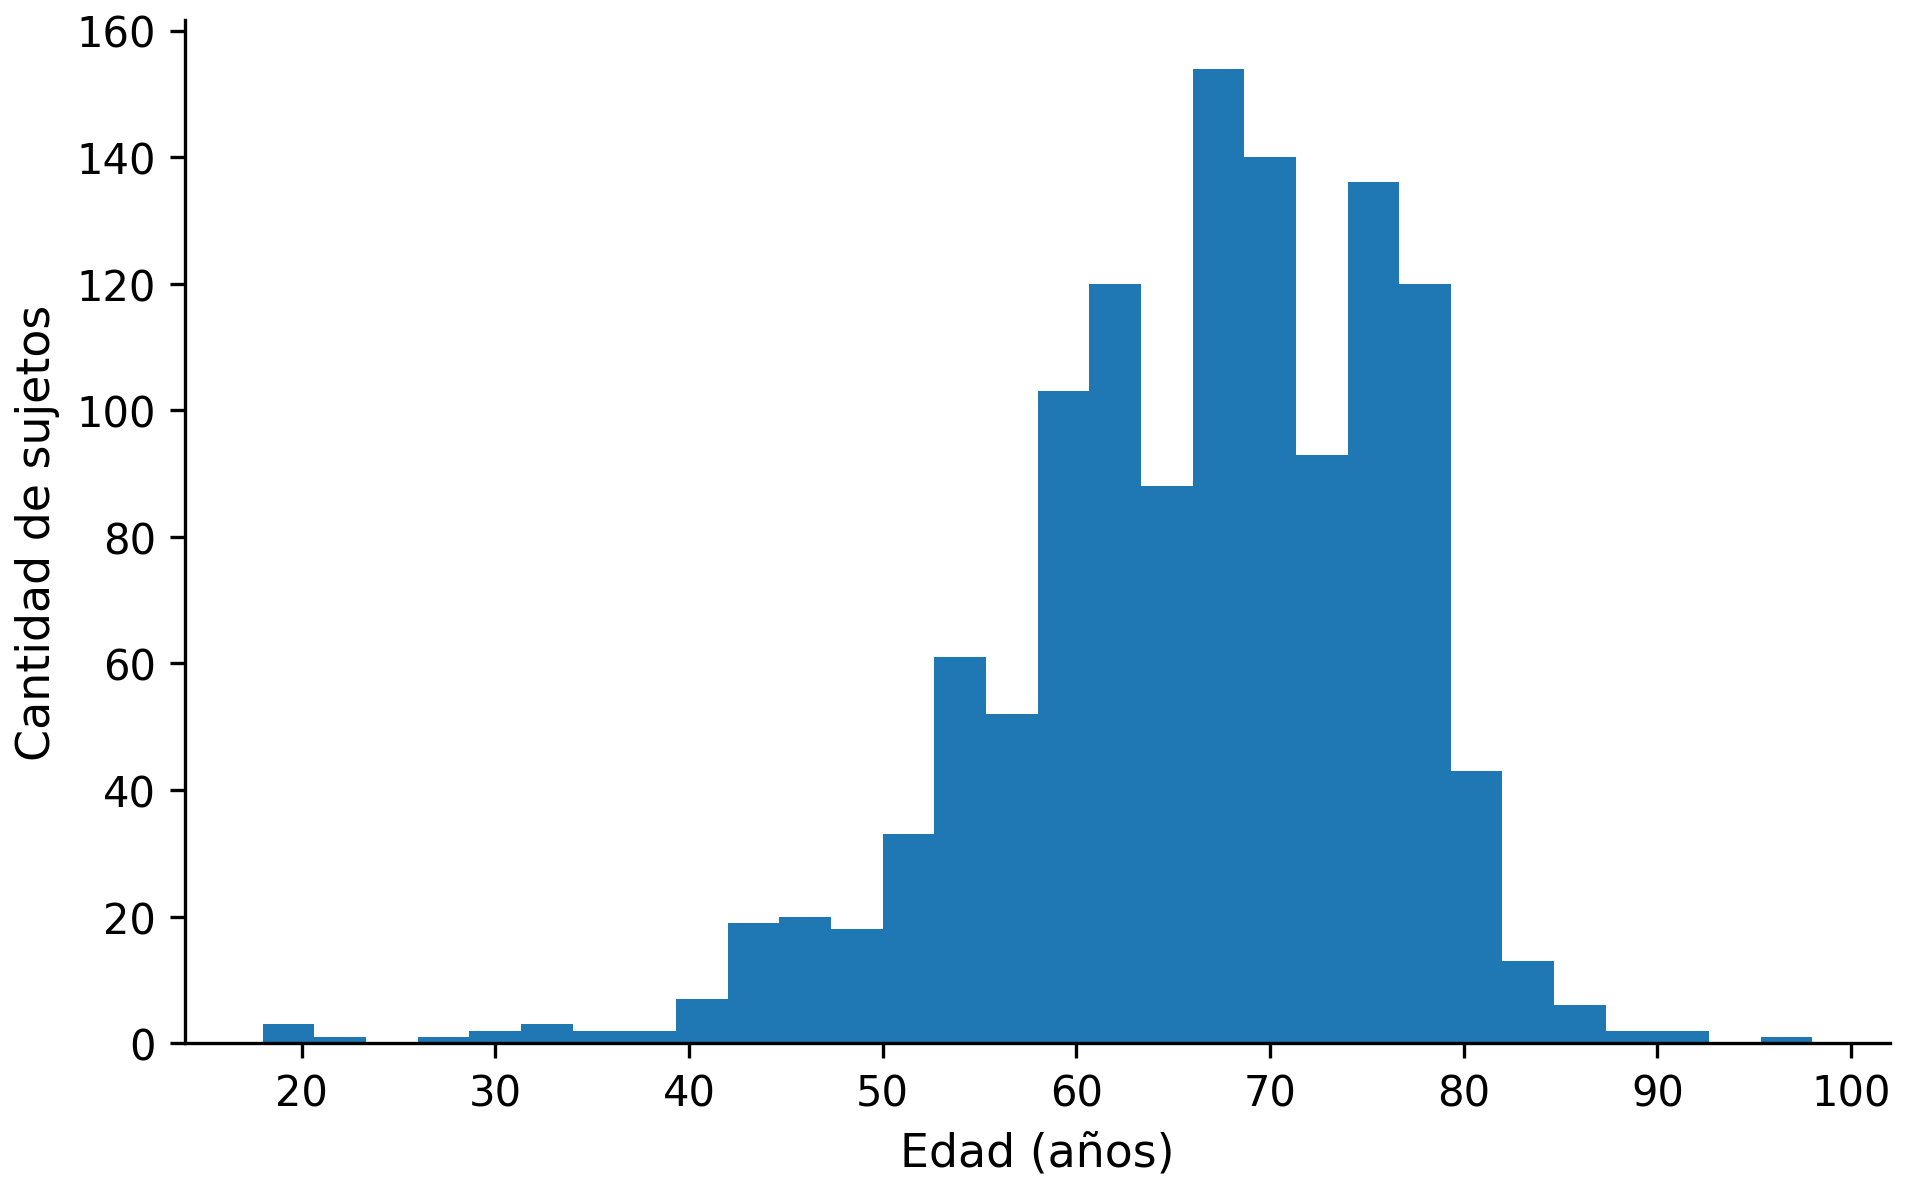
\includegraphics[width=\textwidth]{05_datos_cohorte/images/age_hist.png}
        \caption{Distribución de edades en la cohorte final.}
        \label{fig:age_hist}
    \end{subfigure}
    \hfill
    \begin{subfigure}[t]{0.48\textwidth}
        \centering
        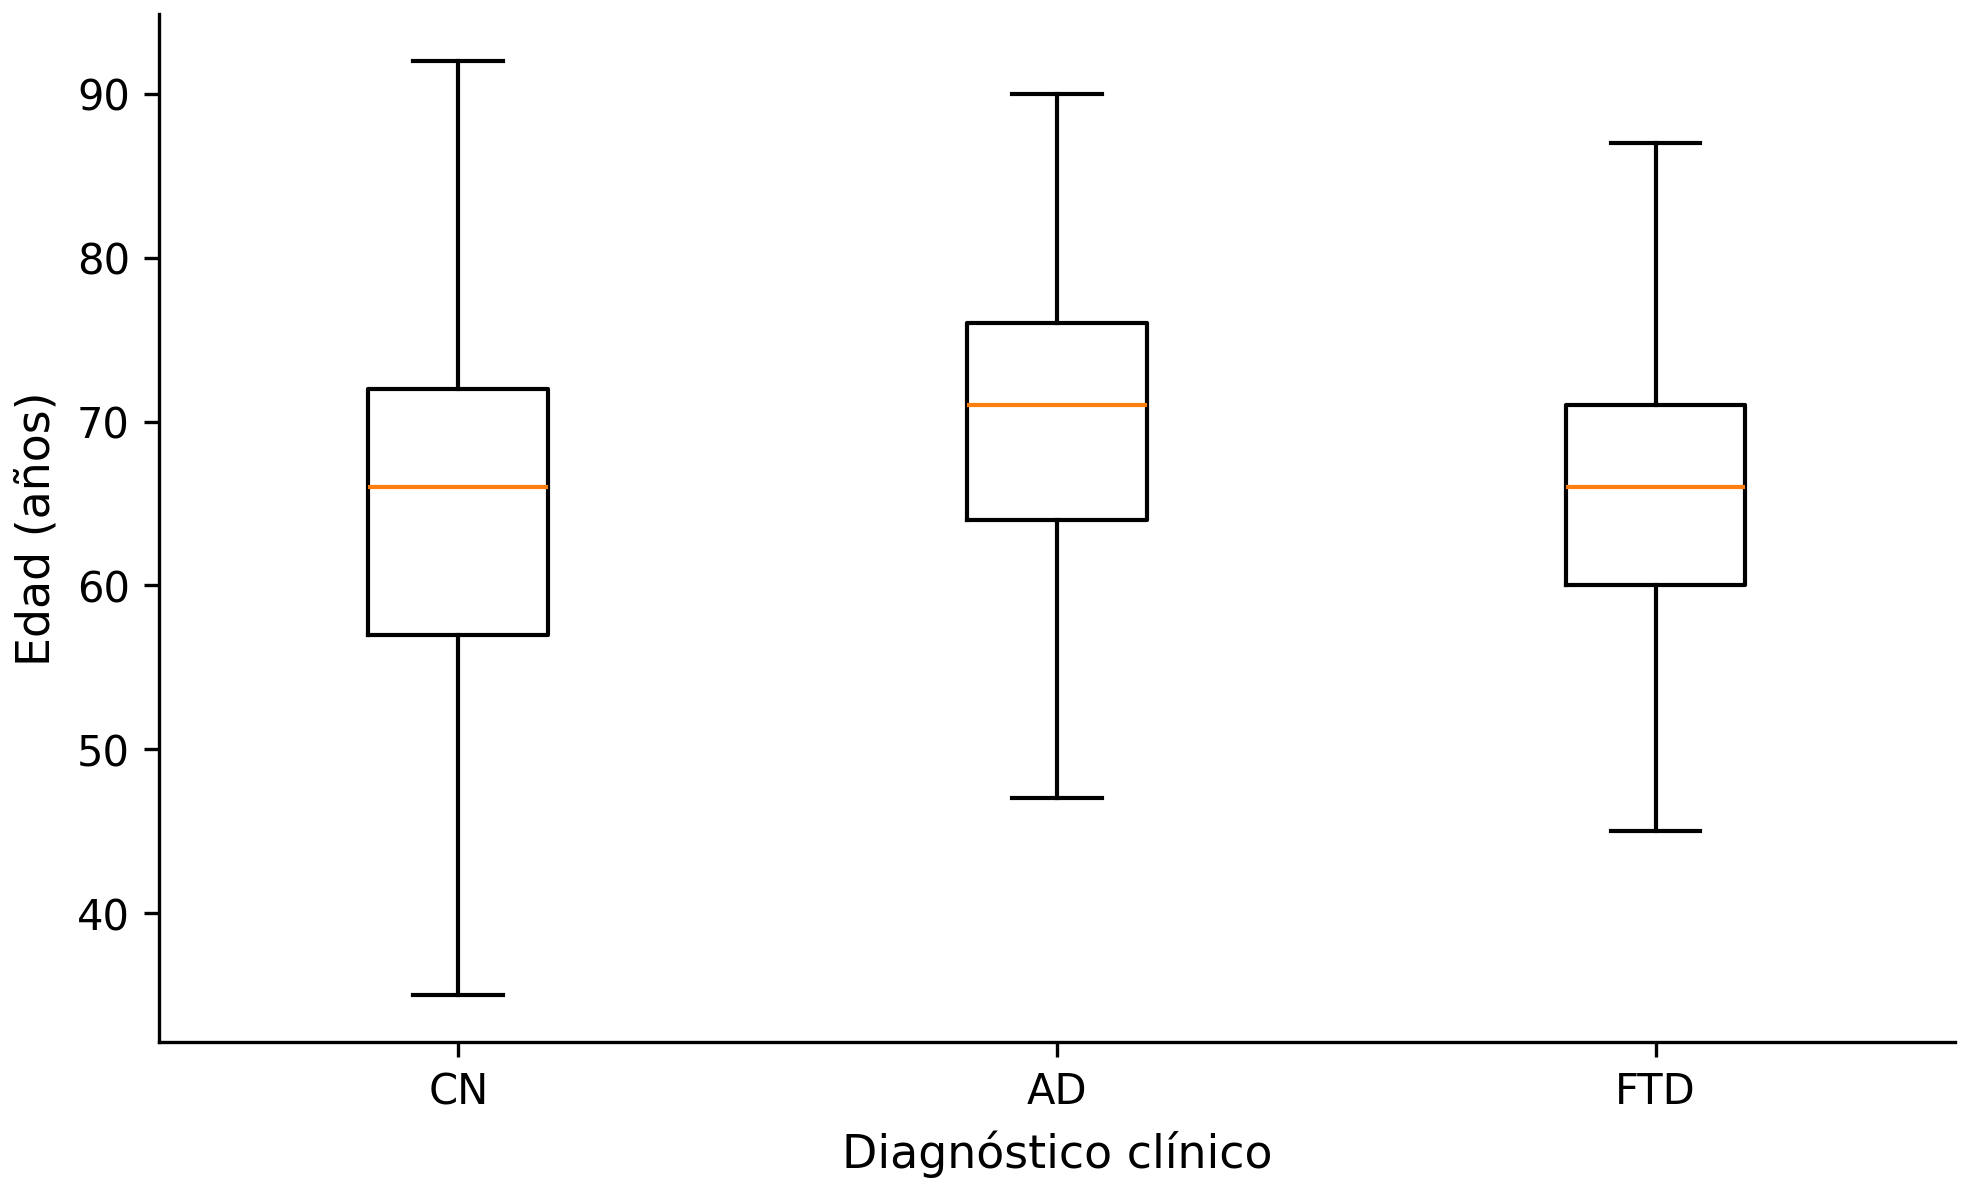
\includegraphics[width=\textwidth]{05_datos_cohorte/images/age_by_diag_box.png}
        \caption{Distribución de la edad por diagnóstico clínico.}
        \label{fig:age_by_diag_box}
    \end{subfigure}
    \caption{Caracterización de la distribución etaria global y estratificada por diagnóstico.}
    \label{fig:age_combined}
\end{figure}


\section{Balance por sexo dentro de cada diagnóstico}
\label{sec:balance_sexo}

Más allá de la distribución global por sexo, es útil evaluar el balance \emph{dentro} de cada diagnóstico. La Figura~\ref{fig:sex_by_diag} muestra la composición porcentual por sexo estratificada por diagnóstico. Se observa un predominio masculino en todos los grupos, más acentuado en CN y AD ($\sim$66\% masculino) y más equilibrado en FTD ($\sim$51\% masculino). Estos desbalances son potencialmente relevantes como factores de confusión y deben tenerse en cuenta al interpretar los resultados del modelo.

\begin{figure}[H]
    \centering
    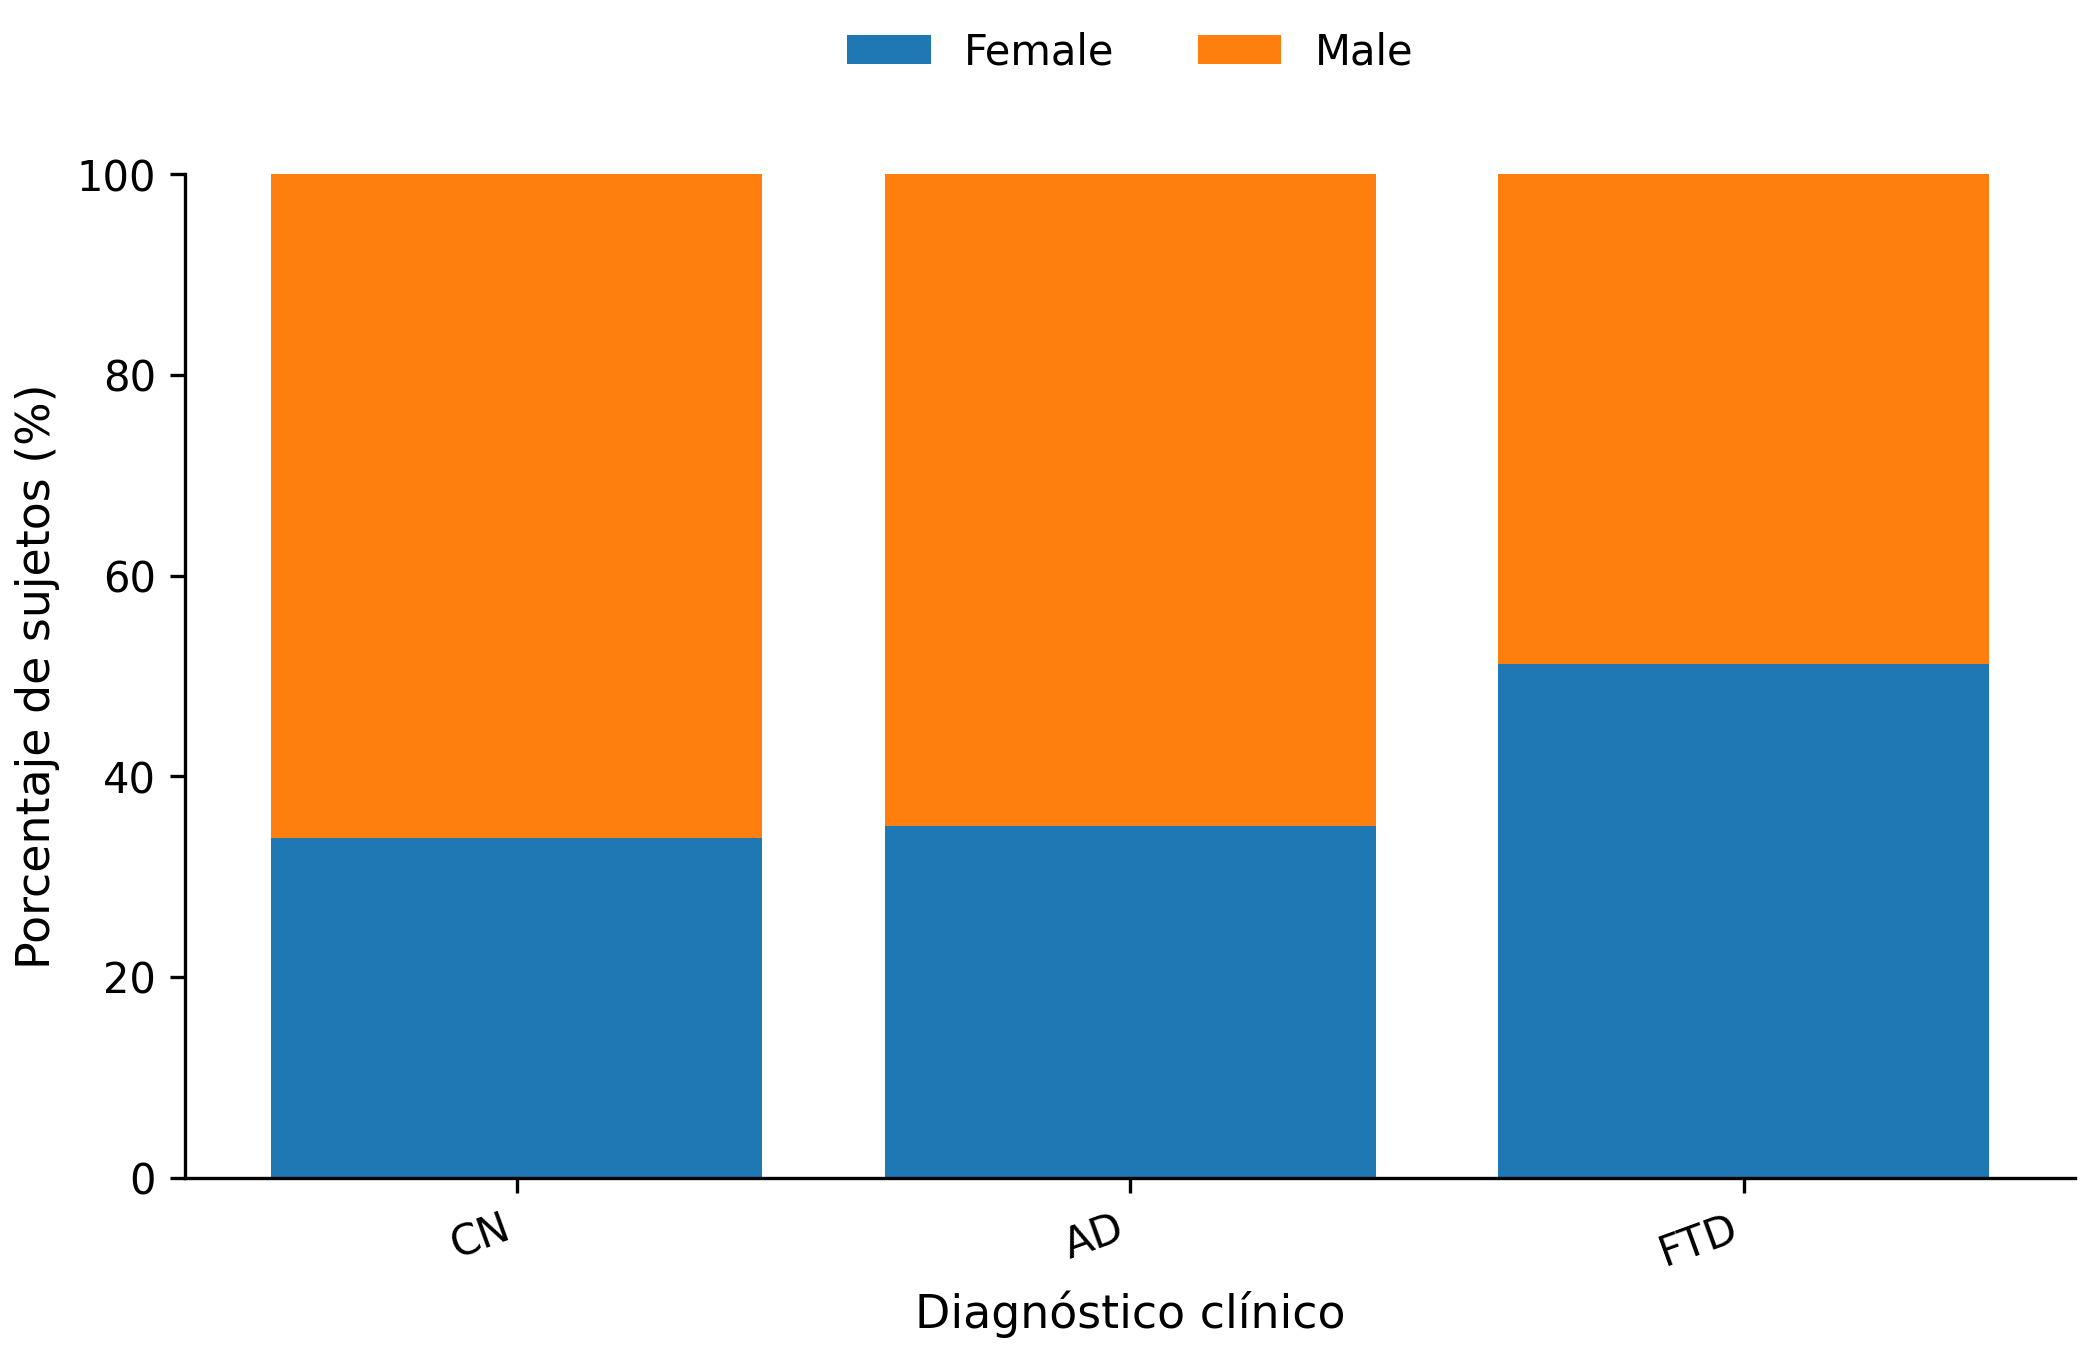
\includegraphics[width=0.82\textwidth]{05_datos_cohorte/images/sex_by_diag_stacked.png}
    \caption{Distribución porcentual por sexo estratificada por diagnóstico clínico.}
    \label{fig:sex_by_diag}
\end{figure}


\section{Variables demográficas adicionales}
\label{sec:demo_adicionales}

Además de la edad, el sexo y el diagnóstico clínico, el archivo de metadatos de RedLaT contiene variables demográficas que no se utilizan como entrada del modelo principal pero resultan relevantes para analizar factores de confusión y moduladores de la predicción de edad cerebral. La Tabla~\ref{tab:demo_availability} resume la disponibilidad de estas variables dentro de la cohorte final.

\begin{table}[H]
\centering
\caption{Disponibilidad de variables demográficas adicionales en la cohorte final ($N = 1245$). Las variables no están completas para todos los sujetos, lo que debe considerarse al interpretar los análisis que las utilizan.}
\label{tab:demo_availability}
\begin{tabular}{llrr}
\toprule
\textbf{Variable} & \textbf{Descripción} & \textbf{Disponibles} & \textbf{\%} \\
\midrule
\texttt{cog\_ed}           & Años de educación formal            & 933  & 74,9\% \\
\texttt{site}              & Sitio de adquisición (centro)       & 941  & 75,6\% \\
\texttt{mri\_scanner\_brand} & Marca del escáner MRI               & 921  & 74,0\% \\
\texttt{mmse\_total}        & Puntuación MMSE                     & 923  & 74,1\% \\
\bottomrule
\end{tabular}
\end{table}

\paragraph{Años de educación (\texttt{cog\_ed}).} Esta variable registra los años de educación formal completados por cada sujeto, y constituye el indicador de nivel socioeconómico más directamente disponible en la cohorte. Los valores oscilan entre 0 y 25 años. Estratificado por diagnóstico, los controles sanos presentan un nivel educativo más alto (media $\approx 16{,}2$ años) que los pacientes con AD ($\approx 12{,}9$ años) y FTD ($\approx 14{,}4$ años). La educación es un factor particularmente relevante en el contexto latinoamericano, donde la variabilidad en el acceso a la educación formal es considerable y puede modular tanto la expresión clínica de la neurodegeneración como el acceso al diagnóstico.

\paragraph{Sitio de adquisición (\texttt{site}).} La cohorte integra datos de múltiples centros de investigación distribuidos en varios países latinoamericanos. Los sitios con mayor representación son Miller ($n = 400$), Matallana ($n = 135$), Slachevsky ($n = 93$), Takada ($n = 89$), Lopera ($n = 88$) y Behrens ($n = 60$). Cada centro utiliza protocolos de adquisición potencialmente distintos, lo que introduce una fuente de variabilidad técnica que puede actuar como factor de confusión en los modelos de predicción.

\paragraph{Marca del escáner MRI (\texttt{mri\_scanner\_brand}).} Los escáneres empleados corresponden a tres fabricantes principales: Siemens ($n = 581$, 63\%), GE ($n = 289$, 31\%) y Philips ($n = 47$, 5\%). Las diferencias en hardware, secuencias de pulso y algoritmos de reconstrucción entre fabricantes pueden producir variaciones sistemáticas en las imágenes, un fenómeno conocido como \textit{scanner bias}. Este sesgo técnico puede manifestarse como diferencias artificiales en las medidas derivadas de la neuroimagen, incluso cuando los cerebros subyacentes son comparables.

La puntuación MMSE (\textit{Mini-Mental State Examination}) se incluye en la tabla por completitud, pero no se utiliza como feature en el pipeline de predicción de edad, ya que es una medida de estado cognitivo que está directamente correlacionada con el diagnóstico clínico y no constituye un predictor independiente del envejecimiento cerebral normal.

Dado que estas variables no están disponibles para la totalidad de la cohorte, los análisis que las utilizan (Capítulo~\ref{chapter:resultados_discusion}) operan sobre subconjuntos de menor tamaño que los $N = 1245$ sujetos del pipeline principal.


\section{Análisis exploratorio}
\label{sec:analisis_exploratorio}

Como control descriptivo previo al modelado, se exploraron relaciones entre la edad y medidas globales derivadas de las dos modalidades de neuroimagen. Para cuantificar estas relaciones se utilizan coeficientes de correlación, que se describen a continuación antes de presentar los resultados.

El \textbf{coeficiente de correlación de Pearson} ($r$) mide la fuerza de la relación lineal entre dos variables. Su valor va de $-1$ a $+1$: un valor de $r = +1$ significa que cuando una variable sube, la otra siempre sube proporcionalmente; $r = -1$ significa que cuando una sube, la otra siempre baja; y $r = 0$ indica que no hay ningún patrón lineal entre ambas. A modo de referencia, valores de $|r|$ entre 0{,}1 y 0{,}3 indican una relación débil, entre 0{,}3 y 0{,}5 moderada, y por encima de 0{,}5 fuerte.

El \textbf{coeficiente de Spearman} ($\rho$) responde a la misma pregunta que el de Pearson, pero no exige que la relación sea una línea recta. En vez de operar sobre los valores numéricos directos, utiliza las posiciones ordenadas (rangos) de los datos, lo que lo hace más resistente a valores extremos y capaz de detectar relaciones curvas o no lineales. Su interpretación es análoga: $\rho = +1$ indica una relación monótona creciente perfecta, $\rho = -1$ decreciente perfecta, y $\rho = 0$ ausencia de tendencia.

El \textbf{valor $p$} acompaña a ambos coeficientes e indica la probabilidad de que la relación observada se deba al azar. Un $p$ bajo significa que es muy improbable que el patrón sea una coincidencia. Por convención, si $p < 0{,}05$ se dice que el resultado es \textit{estadísticamente significativo}: podemos confiar en que la relación detectada es real y no un artefacto del muestreo.

Estas métricas se utilizan a lo largo de este capítulo y del Capítulo~\ref{chapter:resultados_discusion} para evaluar asociaciones entre variables.

\subsection{Edad y volumen de materia gris}

La Figura~\ref{fig:corr_age_gm} muestra la relación entre la edad y el volumen promedio de materia gris por sujeto. Para cada persona, este valor se calcula promediando los 116 volúmenes regionales de materia gris (uno por cada región del atlas AAL), obteniendo un único número que resume la cantidad global de materia gris en su cerebro.

Se observa una correlación negativa moderada (Pearson $r = -0{,}30$, $p < 0{,}001$), lo que significa que las personas de mayor edad tienden a tener menos materia gris. El coeficiente de Spearman ($\rho = -0{,}24$) confirma esta tendencia. Este resultado es consistente con la evidencia de que el volumen de materia gris disminuye progresivamente con la edad (véase Sección~\ref{sec:bases_neuro} del Capítulo~\ref{chapter:marco_teorico}). La dispersión considerable indica que, si bien la tendencia global es clara, existe una marcada variabilidad entre individuos: dos personas de la misma edad pueden tener cantidades de materia gris bastante diferentes.

\begin{figure}[H]
    \centering
    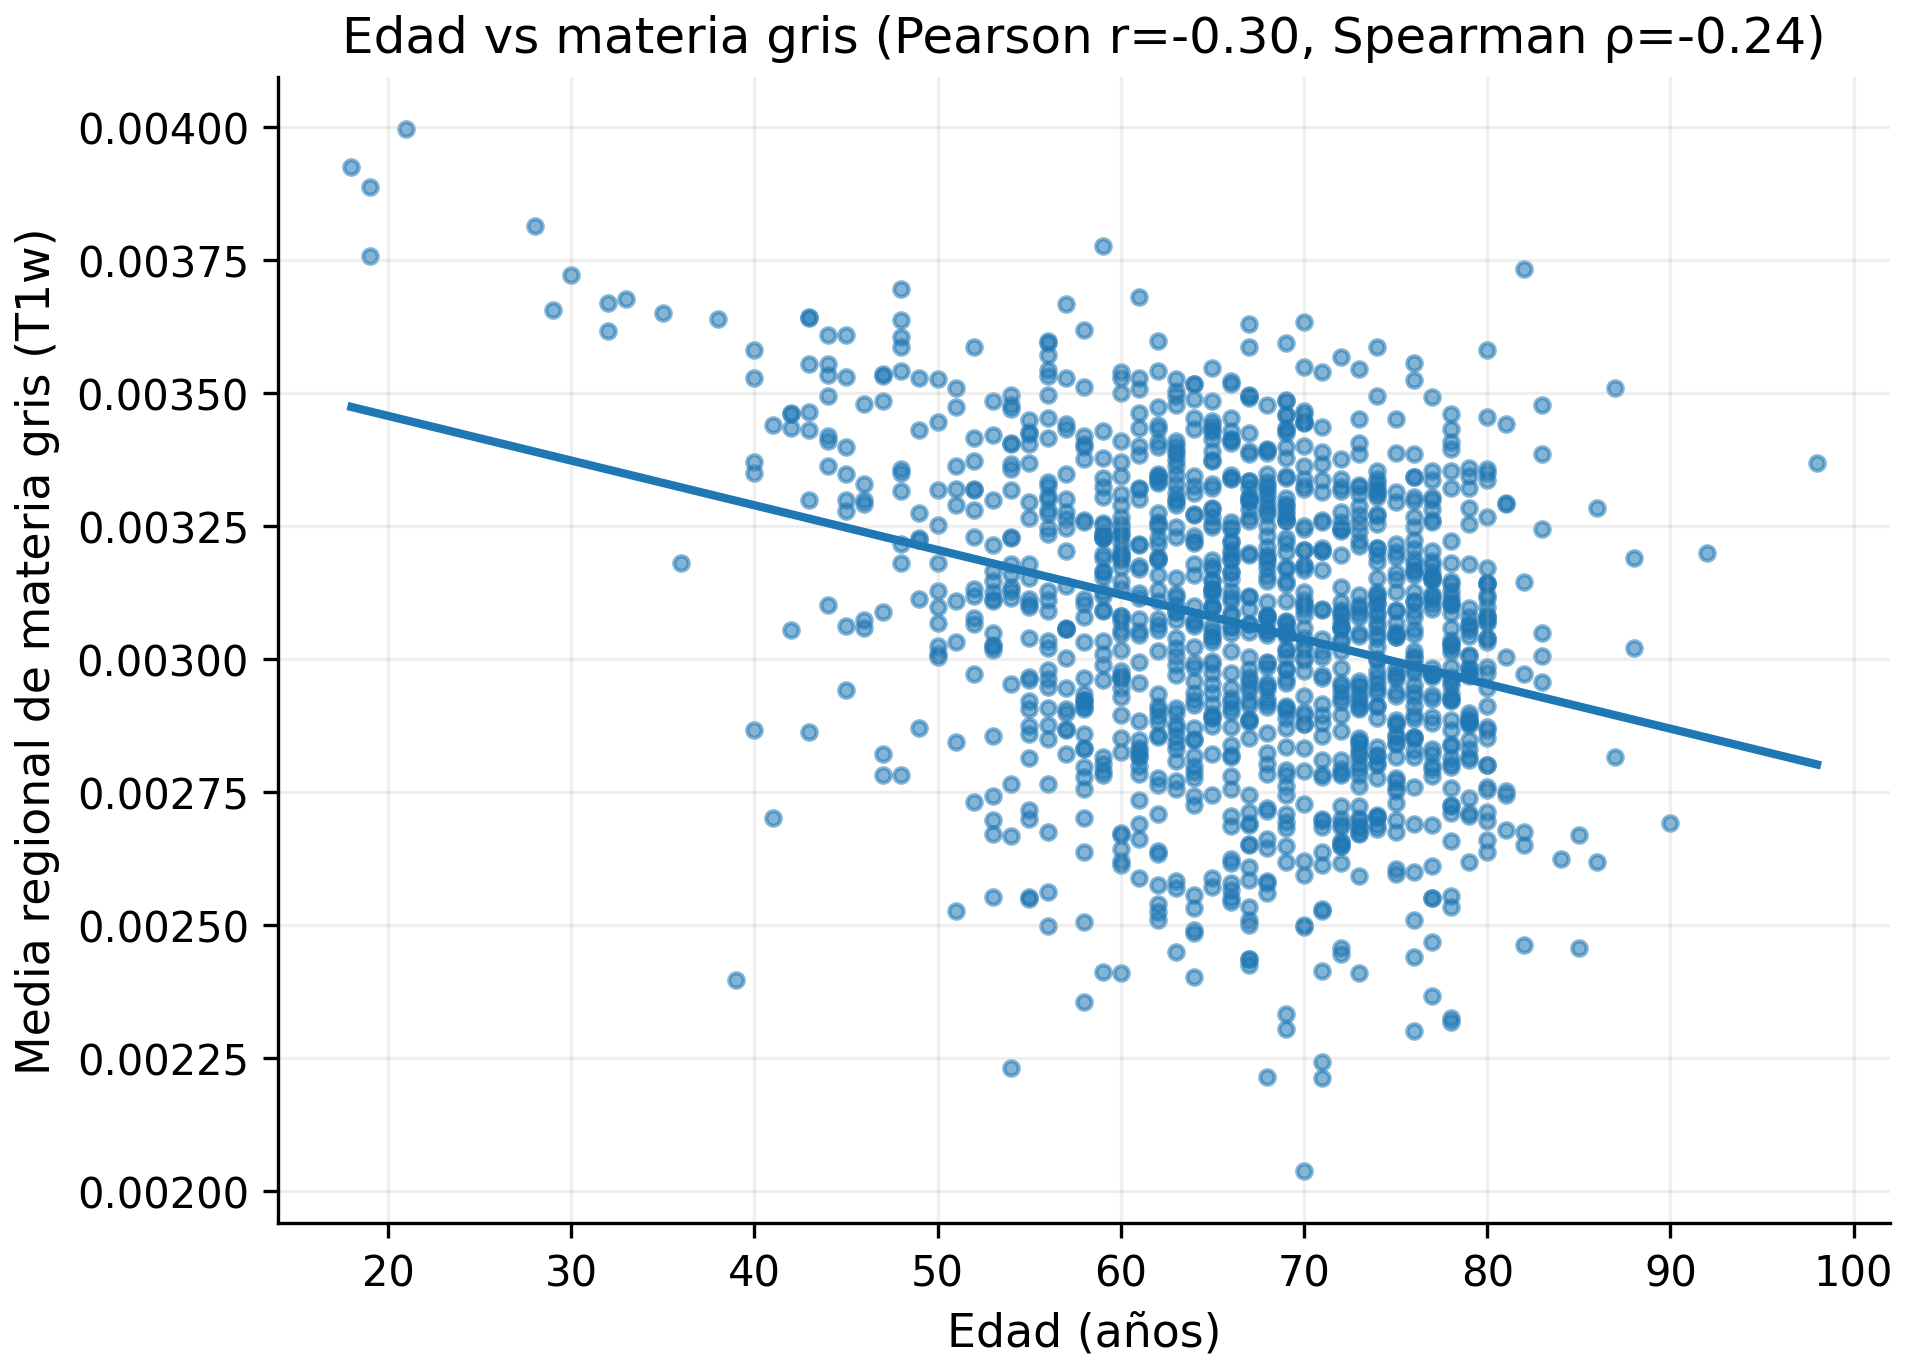
\includegraphics[width=0.78\textwidth]{05_datos_cohorte/images/corr_age_gmmean.png}
    \caption{Edad versus promedio regional de materia gris (T1w). Cada punto corresponde a un sujeto y la recta indica la tendencia lineal.}
    \label{fig:corr_age_gm}
\end{figure}

\subsection{Edad y conectividad funcional global}

De manera complementaria, la Figura~\ref{fig:corr_age_fc} evalúa una medida global simplificada de conectividad funcional: para cada sujeto se calcula el promedio de las correlaciones absolutas entre todos los pares de regiones cerebrales de su matriz FC, obteniendo un único número que resume la fuerza general de la conectividad. En este caso, la correlación con la edad es prácticamente nula (Pearson $r \approx 0{,}00$, Spearman $\rho \approx -0{,}01$), lo que indica que esta medida global no captura los efectos del envejecimiento.

Este resultado no implica que la conectividad funcional no contenga información sobre la edad, sino que dicha información probablemente reside en patrones específicos de conectividad entre regiones y no en una medida agregada global. Esta observación justifica el uso de métodos de reducción de dimensionalidad no lineales (como el $\beta$-VAE descrito en la Sección~\ref{sec:beta_vae_theory} del Capítulo~\ref{chapter:marco_teorico}) que pueden capturar relaciones más complejas entre las 6670 conexiones individuales.

\begin{figure}[H]
    \centering
    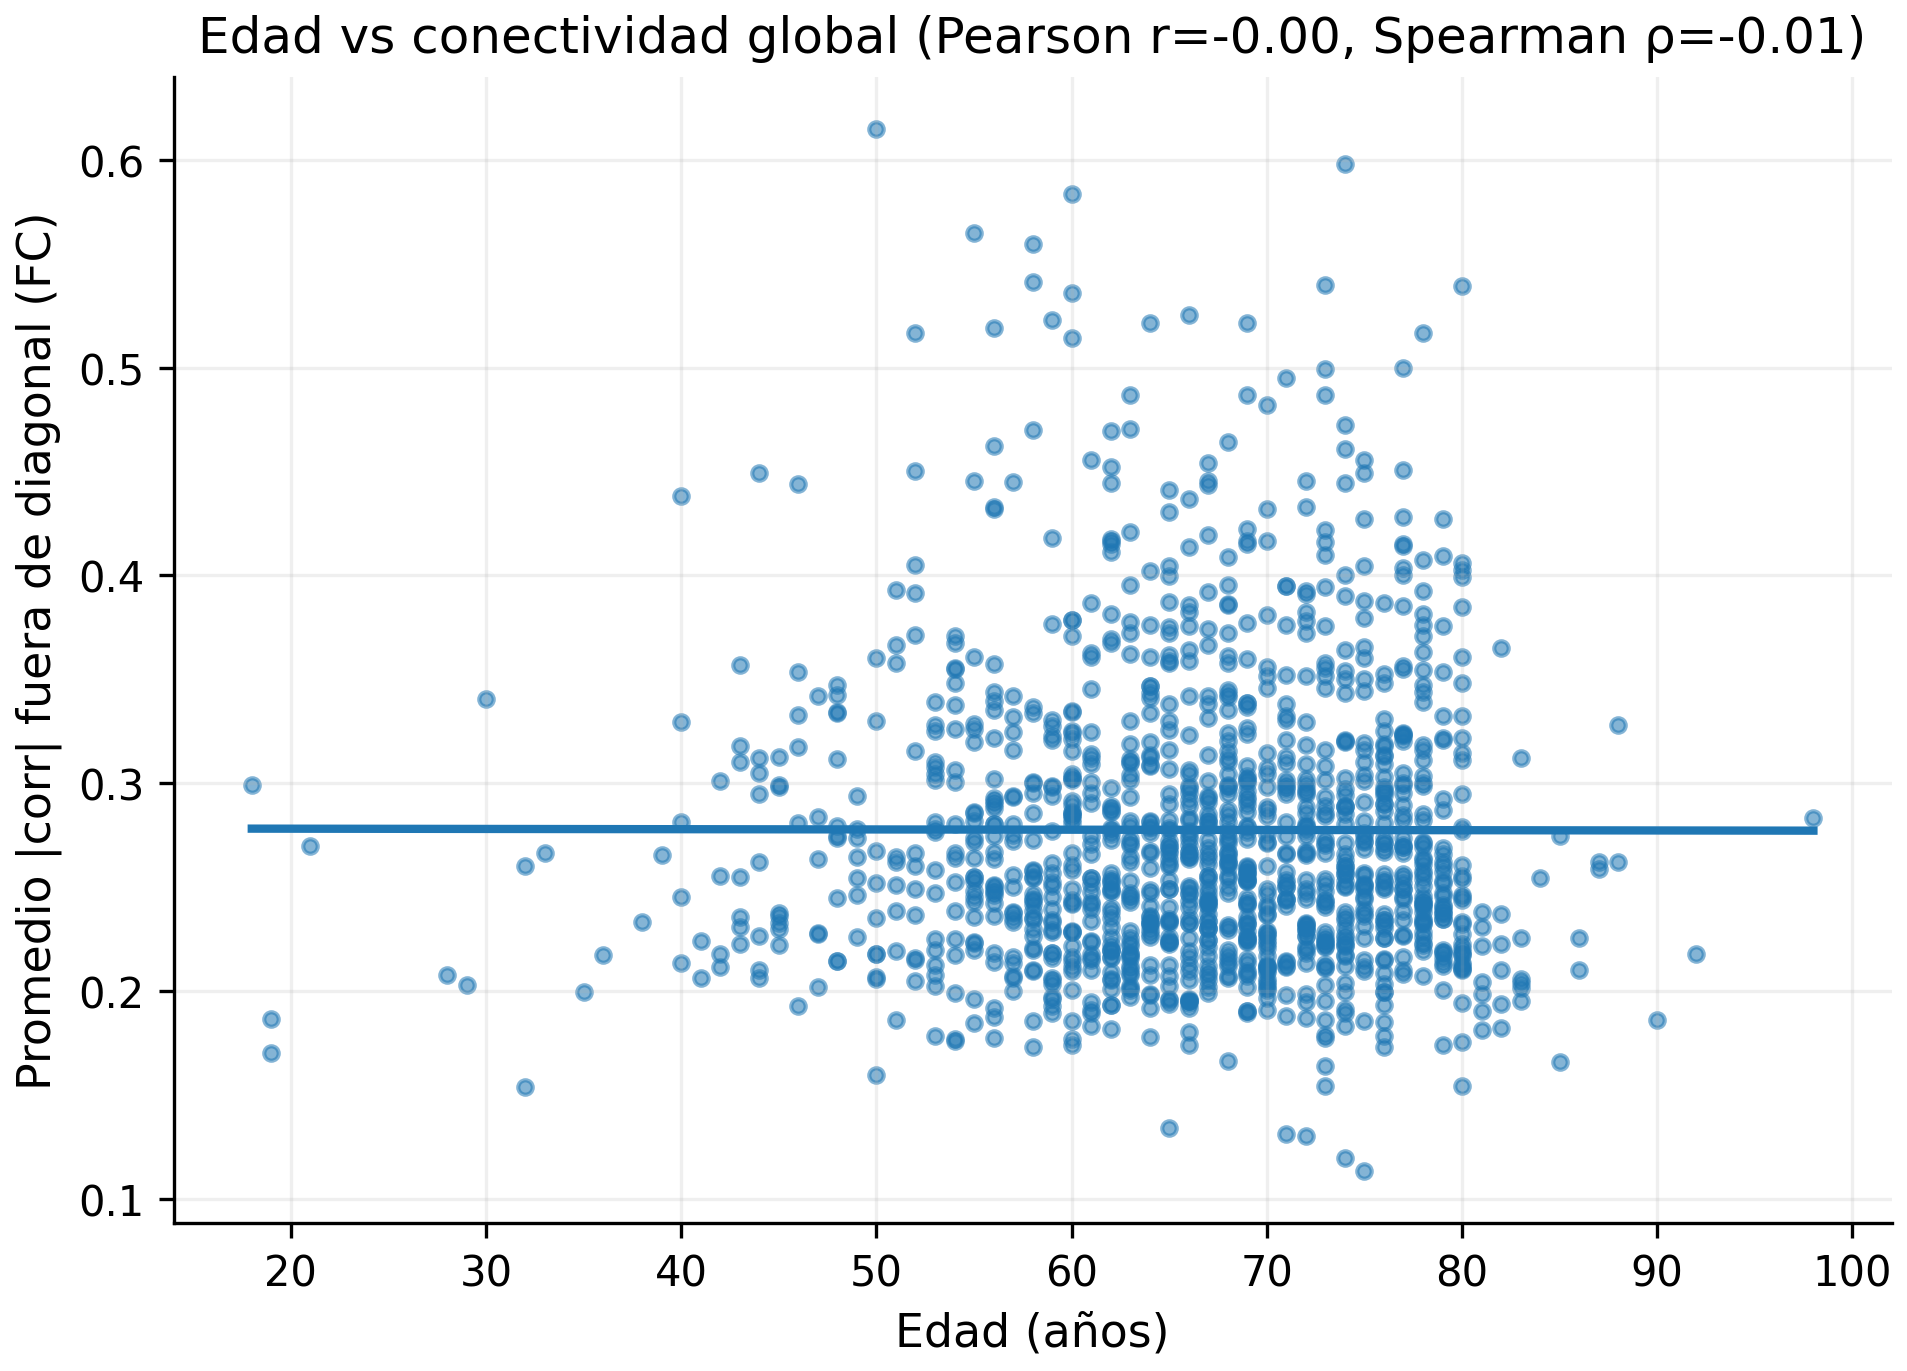
\includegraphics[width=0.78\textwidth]{05_datos_cohorte/images/corr_age_fcmean.png}
    \caption{Edad versus conectividad funcional global (promedio de $|corr|$ fuera de la diagonal). La ausencia de correlación sugiere que los efectos del envejecimiento en FC no se reflejan en una métrica agregada.}
    \label{fig:corr_age_fc}
\end{figure}


\section{Consideraciones poblacionales}
\label{sec:consideraciones_poblacionales}

El uso de una cohorte latinoamericana permite estudiar el envejecimiento cerebral y la neurodegeneración en un contexto poblacional distinto al de cohortes de referencia como ADNI o UK Biobank. Factores asociados a diversidad genética, condiciones de vida, acceso a sistemas de salud y contexto sociocultural podrían contribuir a la variabilidad interindividual observada en medidas funcionales y estructurales. La heterogeneidad en los niveles educativos y en los protocolos de adquisición entre centros, descritas en la Sección~\ref{sec:demo_adicionales}, añade una fuente de variabilidad propia de cohortes multicéntricas latinoamericanas, cuyo impacto sobre la predicción de edad se cuantifica en el Capítulo~\ref{chapter:resultados_discusion}. En conjunto, los análisis presentados en este capítulo describen las principales características de la cohorte de estudio y proporcionan el contexto necesario para la metodología empleada en el Capítulo~\ref{chapter:metodologia_pipeline}.
 \cleardoublepage

% Cap 5: Metodología y pipeline
\chapter{Metodología y pipeline de análisis}
\label{chapter:metodologia_pipeline}

En este capítulo se describe en detalle el pipeline desarrollado para la estimación de la edad cerebral a partir de datos multimodales de neuroimagen. El diseño del pipeline responde a los conceptos teóricos presentados en el Capítulo~\ref{chapter:marco_teorico} y opera sobre la cohorte descrita en el Capítulo~\ref{chapter:datos_cohorte}. A lo largo de las secciones siguientes se presentan las decisiones de diseño adoptadas en cada etapa, junto con su justificación técnica.

\section{Visión general del pipeline}
\label{sec:pipeline_overview}

El pipeline propuesto sigue una arquitectura en dos etapas en cuanto al \textit{flujo de datos}: una primera etapa de reducción de dimensionalidad no supervisada, donde un autoencoder variacional comprime las matrices de conectividad funcional en representaciones latentes compactas, y una segunda etapa de predicción supervisada, donde un modelo XGBoost recibe las representaciones latentes junto con datos estructurales T1w para predecir la edad del sujeto. Antes de entrenar el pipeline en esta configuración, los hiperparámetros de ambos componentes se determinan en una fase previa de optimización: los del $\beta$-VAE mediante \textit{optimización de hiperparámetros con objetivo downstream} (Sección~\ref{sec:optuna_vae}), y los del XGBoost mediante una búsqueda independiente con Optuna una vez fijados los embeddings (Sección~\ref{sec:optuna_xgb}), como se detalla más adelante en este capítulo.

La Figura~\ref{fig:pipeline_general} presenta un diagrama general del flujo de procesamiento.

\begin{figure}[H]
\centering
\begin{tikzpicture}[
    node distance=1.4cm and 1.2cm,
    block/.style={
        rectangle, draw, rounded corners,
        text width=3.2cm, minimum height=1cm,
        align=center, font=\small
    },
    data/.style={
        rectangle, draw, dashed, rounded corners,
        text width=2.8cm, minimum height=0.8cm,
        align=center, font=\small, fill=gray!10
    },
    arrow/.style={-{Stealth[length=3mm]}, thick}
]

% Row 1: Data sources
\node[data] (fc) {Matrices FC\\(116$\times$116)};
\node[data, right=2.5cm of fc] (t1w) {Volúmenes T1w\\(116 regiones)};

% Row 2: Preprocessing
\node[block, below=of fc] (preproc) {Fisher $z$ +\\vectorización\\(6670 dims)};

% Row 3: VAE
\node[block, below=of preproc] (vae) {$\beta$-VAE\\Encoder};
\node[data, below=of vae] (emb) {Embeddings $\mu$\\(64 dims)};

% Row 4: Concatenation
\node[block, below=1.8cm of emb, xshift=1.3cm] (concat) {Concatenación\\de features\\(180 dims)};

% Row 5: XGBoost
\node[block, below=of concat] (xgb) {XGBoost\\Regressor};

% Row 6: Output
\node[data, below=of xgb] (pred) {Edad predicha\\$\hat{y}$};

% Arrows
\draw[arrow] (fc) -- (preproc);
\draw[arrow] (preproc) -- (vae);
\draw[arrow] (vae) -- (emb);
\draw[arrow] (emb) -- (concat);
\draw[arrow] (t1w) |- (concat);
\draw[arrow] (concat) -- (xgb);
\draw[arrow] (xgb) -- (pred);

\end{tikzpicture}
\caption{Diagrama general del pipeline de estimación de edad cerebral. Las matrices de conectividad funcional se comprimen mediante un $\beta$-VAE en representaciones latentes de 64 dimensiones. Estas se concatenan con 116 features estructurales T1w para alimentar un modelo XGBoost que predice la edad.}
\label{fig:pipeline_general}
\end{figure}

La combinación de ambas modalidades busca capturar información complementaria sobre el envejecimiento cerebral: la conectividad funcional refleja patrones de comunicación entre regiones, mientras que los volúmenes T1w aportan información sobre la estructura anatómica del cerebro. Esta estrategia multimodal está motivada por evidencia previa que sugiere que ambas fuentes contribuyen de manera diferente a la predicción de la edad cerebral \cite{erus2015imaging, groves2012benefits}.

\section{Preprocesamiento de los datos}
\label{sec:preprocesamiento}

\subsection{Vectorización y transformación de las matrices de conectividad funcional}

Como se describió en el Capítulo~\ref{chapter:marco_teorico}, cada sujeto dispone de una matriz de conectividad funcional de $116 \times 116$. Dado que esta matriz es simétrica y la diagonal no aporta información, se extrae el triángulo superior sin diagonal, obteniendo un vector de $\frac{116 \times 115}{2} = 6670$ valores por sujeto.

Antes de utilizar estos vectores como entrada del modelo, se aplica la transformación Fisher $z$ (véase la Sección~\ref{sec:fisher_z} del Capítulo~\ref{chapter:marco_teorico}), que convierte los coeficientes de correlación en valores con distribución aproximadamente normal sobre toda la recta real. Esta transformación es una práctica estándar en el análisis de conectividad funcional en neuroimagen \cite{fisher1921probable} y favorece la estabilidad numérica durante el entrenamiento de las redes neuronales.

\subsection{Datos estructurales T1w}

Los datos estructurales T1w comprenden los 116 volúmenes regionales de materia gris descritos en el Capítulo~\ref{chapter:datos_cohorte}.

Durante la construcción de la cohorte se identificó que algunos sujetos presentaban múltiples entradas en los datos T1w, correspondientes a distintas sesiones de escaneo. Para resolver esta duplicidad se promedian las columnas numéricas de todas las entradas asociadas a un mismo sujeto. Esta decisión es conservadora y evita introducir criterios arbitrarios sobre cuál sesión es más representativa.

\section{División de los datos}
\label{sec:division_datos}

En este trabajo se emplean dos niveles de separación, cuyas bases conceptuales se presentan en la Sección~\ref{sec:validacion_evaluacion} del Capítulo~\ref{chapter:marco_teorico}: una partición holdout para la evaluación final y una validación cruzada $K$-Fold para la selección de hiperparámetros.

\subsection{Partición holdout estratificada}

Los $N = 1245$ sujetos de la cohorte se dividen en dos conjuntos disjuntos:
\begin{itemize}
    \item \textbf{Trainval} (90\%, $n = 1120$): utilizado para el entrenamiento de modelos y la selección de hiperparámetros.
    \item \textbf{Test} (10\%, $n = 125$): reservado exclusivamente para la evaluación final. Este conjunto no participa en ninguna decisión de diseño ni de optimización.
\end{itemize}

La partición se realiza mediante muestreo estratificado por la combinación de sexo y diagnóstico clínico (CN, AD, FTD), lo que garantiza que las proporciones de cada subgrupo se mantengan aproximadamente iguales en ambos conjuntos.

\subsection{Validación cruzada $K$-Fold}
\label{sec:kfold}

Dentro del conjunto trainval, se emplea validación cruzada con $K = 5$ folds. Los índices de los folds se generan una única vez a partir de la semilla aleatoria y se almacenan para su reutilización en todas las etapas del pipeline. Esto garantiza que las distintas configuraciones de hiperparámetros sean evaluadas sobre exactamente los mismos subconjuntos de datos, haciendo las comparaciones justas y reproducibles.


\section{Reducción de dimensionalidad: $\beta$-VAE}
\label{sec:beta_vae}

La primera etapa del pipeline consiste en comprimir los vectores de conectividad funcional de 6670 dimensiones en representaciones latentes compactas, utilizando la variante del autoencoder variacional $\beta$-VAE (véase la Sección~\ref{sec:beta_vae_theory} del Capítulo~\ref{chapter:marco_teorico}). El objetivo de esta etapa es obtener representaciones de baja dimensión que capturen los patrones relevantes de la conectividad funcional relacionados con el envejecimiento cerebral.

\subsection{Configuración del $\beta$-VAE}

El valor de $\beta$ se determina mediante optimización automática de hiperparámetros (Sección~\ref{sec:optuna_vae}), obteniendo un valor final de $\beta = 0{,}057$. Este valor, considerablemente menor que 1, indica que el pipeline prioriza la preservación de la información de las matrices FC en el espacio latente por sobre una distribución latente cercana al prior estándar. Esta elección tiene sentido para una tarea downstream de regresión, donde la calidad de la información contenida en los embeddings es más importante que la regularidad geométrica del espacio latente.

Para evitar el colapso posterior durante el entrenamiento (véase la Sección~\ref{sec:beta_vae_theory} del Capítulo~\ref{chapter:marco_teorico}), se emplea la estrategia de calentamiento lineal de $\beta$: durante las primeras $W = 73$ épocas, $\beta$ crece linealmente desde 0 hasta su valor objetivo.

\subsection{Arquitectura del modelo}
\label{sec:vae_architecture}

El encoder y el decoder del $\beta$-VAE están implementados como redes densas (\textit{fully connected}). La elección de una arquitectura densa, en lugar de convolucional, responde a la naturaleza de los datos de entrada: los vectores de conectividad funcional no poseen la estructura espacial local que las capas convolucionales explotan en imágenes, ya que el orden de las 6670 entradas del triángulo superior no codifica relaciones de vecindad espacial.

\paragraph{Encoder.} Recibe el vector de FC transformado ($d = 6670$) y lo procesa a través de una capa oculta de 512 unidades, seguida de dos capas de salida paralelas que producen los parámetros $\mu \in \mathbb{R}^{64}$ y $\log \sigma^2 \in \mathbb{R}^{64}$ de la distribución latente aproximada $q(z|x) = \mathcal{N}(\mu, \sigma^2)$. A partir de estos parámetros se obtiene el vector latente $z$ mediante el truco de reparametrización.

\paragraph{Decoder.} Recibe el vector latente $z \in \mathbb{R}^{64}$ y lo transforma de vuelta al espacio original mediante una capa oculta de 512 unidades, produciendo la reconstrucción $\tilde{x} \in \mathbb{R}^{6670}$.

Ambas redes comparten mecanismos de regularización y normalización en cada capa oculta. Las activaciones se normalizan mediante \textit{Layer Normalization}, que estabiliza el entrenamiento sin depender del tamaño del batch. En una red neuronal, cada capa aplica una \textit{función de activación} que determina cómo se transforma la señal de salida de cada neurona; sin esta función, la red se reduciría a una transformación lineal, limitando su capacidad de modelar relaciones complejas. La función de activación utilizada es ELU (\textit{Exponential Linear Unit}), seleccionada a partir de experimentos preliminares en los que se evaluaron distintas funciones de activación (ReLU, ELU, Sigmoid, entre otras) mediante optimización con Optuna. ELU presenta la ventaja de que, a diferencia de ReLU (que devuelve 0 para cualquier entrada negativa y puede hacer que ciertas neuronas dejen de aprender permanentemente), permite valores de salida ligeramente negativos, lo que favorece la estabilidad del entrenamiento. Para prevenir el sobreajuste se utiliza dropout ($p = 0{,}037$), que desactiva aleatoriamente una fracción de las neuronas durante el entrenamiento, y regularización L2 ($\lambda = 2{,}9 \times 10^{-7}$), que penaliza la magnitud de los pesos.

\paragraph{Función de pérdida de reconstrucción.} Se utiliza el error absoluto medio (MAE) en lugar del error cuadrático medio (MSE), ya que MAE es más robusto frente a valores atípicos en las matrices de conectividad funcional.

La Tabla~\ref{tab:vae_hparams} resume los hiperparámetros del modelo $\beta$-VAE final.

\begin{table}[H]
\centering
\caption{Hiperparámetros del $\beta$-VAE final, obtenidos mediante optimización con Optuna.}
\label{tab:vae_hparams}
\begin{tabular}{ll}
\toprule
\textbf{Hiperparámetro} & \textbf{Valor} \\
\midrule
Dimensión de entrada & 6670 \\
Capas ocultas (encoder / decoder) & [512] \\
Dimensión latente & 64 \\
$\beta_{\text{target}}$ & 0,057 \\
Épocas de warmup ($W$) & 73 \\
Función de reconstrucción & MAE \\
Activación & ELU \\
Normalización & LayerNorm \\
Dropout & 0,037 \\
Regularización L2 & $2{,}9 \times 10^{-7}$ \\
Learning rate & $1{,}89 \times 10^{-3}$ \\
Gradient clipping & 1,0 \\
Batch size & 64 \\
Épocas de entrenamiento & 96 \\
Semilla & 42 \\
\bottomrule
\end{tabular}
\end{table}

\subsection{Optimización de hiperparámetros con objetivo downstream}
\label{sec:optuna_vae}

Un aspecto central del diseño del pipeline es la forma en que se seleccionan los hiperparámetros del $\beta$-VAE. A diferencia de la práctica habitual de optimizar el $\beta$-VAE exclusivamente para minimizar su error de reconstrucción, en este trabajo se adopta un \textit{objetivo downstream}: los hiperparámetros se seleccionan en función de qué tan útiles resultan las representaciones latentes para la tarea de predicción de edad.

La motivación detrás de esta decisión es que un $\beta$-VAE con excelente reconstrucción podría estar capturando información irrelevante para el envejecimiento (como artefactos de movimiento, diferencias de protocolo entre sitios o ruido del escáner). Al evaluar los hiperparámetros según su impacto en la predicción de edad, se fuerza al modelo a aprender representaciones que capturen información relevante al envejecimiento cerebral.

Para esta optimización se utiliza Optuna \cite{akiba2019optuna}, un framework de optimización de hiperparámetros cuyas bases se describen en la Sección~\ref{sec:hpo_theory} del Capítulo~\ref{chapter:marco_teorico}.

La Tabla~\ref{tab:optuna_vae_search} describe el espacio de búsqueda explorado.

\begin{table}[H]
\centering
\caption{Espacio de búsqueda de Optuna para la optimización del $\beta$-VAE.}
\label{tab:optuna_vae_search}
\resizebox{\textwidth}{!}{%
\begin{tabular}{lll}
\toprule
\textbf{Hiperparámetro} & \textbf{Tipo} & \textbf{Rango / Opciones} \\
\midrule
Dimensión latente & Categórico & \{16, 32, 64, 128, 224\} \\
Capas ocultas & Categórico & \{256; 512; 512-256; 1024-512; 1024-512-256\} \\
$\beta$ & Log-uniforme & $[10^{-4},\; 0{,}2]$ \\
Learning rate & Log-uniforme & $[10^{-4},\; 3 \times 10^{-3}]$ \\
Dropout & Uniforme & $[0,\; 0{,}20]$ \\
Épocas de warmup & Entero uniforme & $[10,\; 100]$ \\
Tipo de embedding & Categórico & \{$\mu$,\; $z$\} \\
\bottomrule
\end{tabular}}
\end{table}

\paragraph{Procedimiento de evaluación de cada trial.} Para cada configuración de hiperparámetros propuesta por Optuna, se evalúa su calidad mediante validación cruzada con $K = 5$ folds, utilizando \emph{únicamente} los datos del conjunto trainval; el conjunto de test no participa en esta etapa y se reserva para la evaluación final. En cada iteración $k$ ($k = 1, \ldots, 5$), los datos de trainval se dividen en un conjunto de entrenamiento (4 folds) y uno de validación (1 fold). El procedimiento para cada fold es:

\begin{enumerate}
    \item Entrenar el $\beta$-VAE sobre los datos de FC del conjunto de entrenamiento del fold $k$ (aprendizaje no supervisado; no se utiliza la variable edad). Al finalizar, el encoder funciona como una ``máquina de comprimir'' que transforma cualquier vector FC de 6670 dimensiones en un embedding de 64.
    \item Pasar los datos de FC de \emph{entrenamiento} por el encoder para obtener sus embeddings. Pasar también los datos de FC de \emph{validación} por el mismo encoder para obtener los embeddings de sujetos que el $\beta$-VAE no vio durante su entrenamiento.
    \item Construir los vectores de características concatenando los embeddings con los datos T1w, obteniendo un vector por sujeto tanto para entrenamiento como para validación.
    \item Entrenar un modelo XGBoost con hiperparámetros fijos sobre los vectores de entrenamiento del fold $k$.
    \item Predecir la edad en los sujetos de validación (usando sus embeddings y T1w) y calcular el MAE. Dado que estos sujetos no fueron vistos ni por el $\beta$-VAE ni por XGBoost, el MAE refleja la capacidad real de generalización de esta configuración de hiperparámetros.
\end{enumerate}

El resultado del trial se define como el promedio de los 5 valores de MAE (uno por fold). De este modo, cada configuración de hiperparámetros se evalúa sobre la totalidad de los datos trainval sin que ningún sujeto participe simultáneamente en el entrenamiento y la evaluación. Optuna descarta prematuramente los trials cuyo rendimiento parcial es claramente inferior al de los trials completados, reduciendo el tiempo total de búsqueda.

\paragraph{XGBoost con parámetros fijos durante la búsqueda del $\beta$-VAE.} Durante la optimización del $\beta$-VAE, el XGBoost mantiene hiperparámetros fijos y razonables (no optimizados), actuando como evaluador consistente de la calidad de los embeddings. Si ambos modelos se optimizaran simultáneamente, la búsqueda sería combinatoriamente intratable. La optimización propia de XGBoost se realiza en una etapa posterior (Sección~\ref{sec:optuna_xgb}), una vez que los embeddings del $\beta$-VAE están fijados.

\paragraph{Optimización secuencial en dos etapas.} La decisión de mantener el pipeline como dos módulos separados ($\beta$-VAE + regresor), en lugar de un modelo end-to-end, responde a criterios de tratabilidad computacional e interpretabilidad. El proceso completo de selección de hiperparámetros se estructura en tres fases, ilustradas en la Figura~\ref{fig:optuna_twostage}: (1)~optimización del $\beta$-VAE con un evaluador XGBoost congelado, (2)~optimización del XGBoost con los embeddings fijados del mejor $\beta$-VAE, y (3)~entrenamiento final de ambos modelos sobre la totalidad del conjunto trainval. Esta estructura modular permite además intercambiar el regresor (por ejemplo, sustituir XGBoost por Ridge o SVR, como se evalúa en la Sección~\ref{sec:res_regresores}) sin necesidad de reentrenar el $\beta$-VAE.

\begin{figure}[H]
\centering
\resizebox{\textwidth}{!}{%
\begin{tikzpicture}[
    phase/.style={
        rectangle, draw, rounded corners=4pt,
        minimum width=3cm, minimum height=0.9cm,
        align=center, font=\small\bfseries,
        fill=#1!15, draw=#1!60,
    },
    pstep/.style={
        rectangle, draw, rounded corners=2pt,
        text width=4.2cm, minimum height=0.7cm,
        align=center, font=\footnotesize,
    },
    frozen/.style={
        rectangle, draw, rounded corners=2pt, dashed,
        text width=4.2cm, minimum height=0.7cm,
        align=center, font=\footnotesize, fill=gray!10,
    },
    arr/.style={-Latex, thick},
    darr/.style={-Latex, thick, dashed, gray},
    font=\small,
]

% Phase 1
\node[phase=purple] (p1) at (0, 0) {Etapa 1: Optuna $\beta$-VAE};
\node[pstep, below=0.4cm of p1] (s1a) {Sugerir hiperparámetros $\beta$-VAE\\(latent\_dim, $\beta$, lr, \ldots)};
\node[pstep, below=0.3cm of s1a] (s1b) {Entrenar $\beta$-VAE en fold $k$\\(no supervisado)};
\node[pstep, below=0.3cm of s1b] (s1c) {Extraer embeddings\\del fold de validación};
\node[frozen, below=0.3cm of s1c] (s1d) {Entrenar XGBoost\\(\textit{parámetros fijos})};
\node[pstep, below=0.3cm of s1d] (s1e) {Calcular MAE en validación\\$\rightarrow$ reportar a Optuna};

\draw[arr] (p1) -- (s1a);
\draw[arr] (s1a) -- (s1b);
\draw[arr] (s1b) -- (s1c);
\draw[arr] (s1c) -- (s1d);
\draw[arr] (s1d) -- (s1e);

\draw[darr, bend left=40] (s1e.west) to node[left, font=\scriptsize, text=gray] {$k=1\ldots5$} (s1b.west);

\draw[darr, bend right=55] (s1e.east) to node[left, font=\scriptsize, text=gray] {$\times\,70$} (s1a.east);

\node[below=0.3cm of s1e, font=\footnotesize\bfseries, purple!70!black] (out1) {$\rightarrow$ Mejor configuración $\beta$-VAE};

% Phase 2
\node[phase=orange, right=3.5cm of p1] (p2) at (7, 0) {Etapa 2: Optuna XGBoost};
\node[frozen, below=0.4cm of p2] (s2a) {$\beta$-VAE fijo (mejor de Etapa 1)\\$\rightarrow$ embeddings fijos};
\node[pstep, below=0.3cm of s2a] (s2b) {Sugerir hiperparámetros XGB\\(n\_est, depth, lr, \ldots)};
\node[pstep, below=0.3cm of s2b] (s2c) {Entrenar XGBoost en fold $k$\\con embeddings fijos};
\node[pstep, below=0.3cm of s2c] (s2d) {Calcular MAE en validación\\$\rightarrow$ reportar a Optuna};

\draw[arr] (p2) -- (s2a);
\draw[arr] (s2a) -- (s2b);
\draw[arr] (s2b) -- (s2c);
\draw[arr] (s2c) -- (s2d);

\draw[darr, bend left=40] (s2d.west) to node[left, font=\scriptsize, text=gray] {$k=1\ldots5$} (s2c.west);

\draw[darr, bend right=55] (s2d.east) to node[right, font=\scriptsize, text=gray] {$\times\,100$} (s2b.east);

\node[below=0.3cm of s2d, font=\footnotesize\bfseries, orange!70!black] (out2) {$\rightarrow$ Mejor configuración XGBoost};

% Phase 3
\node[phase=teal, right=3.5cm of p2] (p3) at (14, 0) {Etapa 3: Modelo final};
\node[pstep, below=0.4cm of p3, fill=purple!8] (s3a) {Entrenar $\beta$-VAE final\\(best params, todo trainval)};
\node[pstep, below=0.3cm of s3a] (s3b) {Extraer embeddings finales\\(todo trainval + test)};
\node[pstep, below=0.3cm of s3b, fill=orange!8] (s3c) {Entrenar XGBoost final\\(best params, todo trainval)};
\node[pstep, below=0.3cm of s3c, fill=teal!10] (s3d) {Evaluar en conjunto\\de test holdout};

\draw[arr] (p3) -- (s3a);
\draw[arr] (s3a) -- (s3b);
\draw[arr] (s3b) -- (s3c);
\draw[arr] (s3c) -- (s3d);

% Arrows between phases
\draw[arr, purple!60, very thick] (out1.east) -- ++(1.2,0) |- (p2.west);
\draw[arr, orange!60, very thick] (out2.east) -- ++(1.2,0) |- (p3.west);

% Labels
\node[below=0.15cm of s3d, font=\footnotesize\bfseries, teal!70!black] {$\rightarrow$ MAE, $R^2$, Pearson $r$};

% Legend
\node[frozen, text width=2.5cm, minimum height=0.5cm] at (3.5, -7.5) (leg1) {\footnotesize Componente fijo};
\node[pstep, text width=2.5cm, minimum height=0.5cm, right=0.5cm of leg1] (leg2) {\footnotesize Componente activo};

\end{tikzpicture}}
\caption{Proceso de optimización de hiperparámetros en dos etapas. Los componentes congelados se indican con borde discontinuo. Los bucles internos ($k=1\ldots5$) representan la validación cruzada dentro de cada trial, y los bucles externos representan las iteraciones de Optuna (70 trials para el $\beta$-VAE, 100 para XGBoost).}
\label{fig:optuna_twostage}
\end{figure}

En total, se ejecutaron 70 trials de Optuna para la optimización del $\beta$-VAE. El mejor trial obtuvo un MAE promedio de 6,43 años en validación cruzada.


\subsection{Entrenamiento final y extracción de embeddings}
\label{sec:vae_final}

Una vez determinados los hiperparámetros óptimos, se entrena el $\beta$-VAE final sobre la totalidad del conjunto trainval ($n = 1120$ sujetos), sin reservar datos para validación interna. El objetivo es maximizar la cantidad de datos disponibles para el aprendizaje de representaciones.

El número de épocas de entrenamiento se determina a partir de la validación cruzada: durante la optimización con Optuna, se registra la época en la que cada fold alcanzó su mejor pérdida de reconstrucción en validación. Se toma la mediana de estas épocas como referencia para el entrenamiento final, resultando en 96 épocas. La mediana se prefiere sobre la media por su robustez frente a folds atípicos.

\paragraph{Calidad de reconstrucción.} El $\beta$-VAE final alcanzó una correlación de Pearson promedio de $0{,}79$ y una similitud coseno promedio de $0{,}87$ sobre el conjunto trainval, lo que indica que la estructura de las matrices FC se preserva en un grado sustancial tras la compresión. Estos valores se analizan en mayor detalle en el Capítulo~\ref{chapter:resultados_discusion}.

\paragraph{Extracción de embeddings.} Una vez entrenado el modelo, el decoder se descarta y solo se conserva el encoder, ya que el objetivo no es reconstruir las matrices FC sino obtener representaciones compactas para la etapa de predicción. Se extraen los embeddings pasando los vectores de FC por el encoder y tomando la media $\mu$ de la distribución latente como representación de cada sujeto. Si bien la búsqueda de hiperparámetros con Optuna evaluó tanto $\mu$ como la muestra estocástica $z = \mu + \sigma \odot \epsilon$, y el trial óptimo utilizó $z$, se optó por emplear $\mu$ en el pipeline final. Esta decisión se fundamenta en que $\mu$ es determinístico: el mismo sujeto siempre produce el mismo embedding, lo cual garantiza la reproducibilidad de los resultados y la estabilidad de la etapa de predicción posterior. Los embeddings resultantes tienen dimensión 64 para cada sujeto.

\section{Modelo de predicción: XGBoost}
\label{sec:xgboost_pipeline}

La segunda etapa del pipeline utiliza XGBoost como modelo de regresión para predecir la edad a partir de la combinación de representaciones latentes del $\beta$-VAE y features estructurales T1w.

\subsection{Construcción del vector de características}

Para cada sujeto, el vector de entrada al modelo XGBoost se construye concatenando dos bloques de features:
\begin{itemize}
    \item \textbf{Embeddings del $\beta$-VAE}: 64 dimensiones, obtenidas del encoder como se describió en la Sección~\ref{sec:vae_final}. Estas representaciones codifican patrones de conectividad funcional relevantes para la predicción.
    \item \textbf{Volúmenes T1w}: 116 dimensiones, correspondientes a los volúmenes regionales de materia gris del atlas AAL.
\end{itemize}

El vector resultante tiene $64 + 116 = 180$ dimensiones por sujeto. Esta concatenación de features permite que el modelo XGBoost explote conjuntamente la información funcional y estructural.

Es relevante notar que el sexo del sujeto no se incluye en la configuración final del modelo, a pesar de que fue evaluado como feature adicional. Como se muestra en la Sección~\ref{sec:ablaciones}, su inclusión no mejoró el rendimiento (MAE 5,70 vs.\ 5,62 sin sexo), posiblemente debido al tamaño reducido de la muestra.

\subsection{Optimización de hiperparámetros}
\label{sec:optuna_xgb}

Los hiperparámetros de XGBoost se optimizan mediante una búsqueda independiente con Optuna, utilizando validación cruzada con los mismos 5 folds definidos previamente. Los embeddings del $\beta$-VAE final se mantienen fijos durante esta etapa, de modo que la búsqueda se centra exclusivamente en los parámetros del modelo de regresión.

Se ejecutaron 100 trials, obteniendo un MAE promedio de 6,36 años en validación cruzada para la mejor configuración. La Tabla~\ref{tab:xgb_hparams} presenta los hiperparámetros finales seleccionados.

\begin{table}[H]
\centering
\caption{Hiperparámetros del modelo XGBoost final, obtenidos mediante optimización con Optuna.}
\label{tab:xgb_hparams}
\begin{tabular}{ll}
\toprule
\textbf{Hiperparámetro} & \textbf{Valor} \\
\midrule
Número de árboles (\texttt{n\_estimators}) & 2103 \\
Profundidad máxima (\texttt{max\_depth}) & 6 \\
Tasa de aprendizaje (\texttt{learning\_rate}) & 0,011 \\
Fracción de muestras por árbol (\texttt{subsample}) & 0,502 \\
Fracción de features por árbol (\texttt{colsample\_bytree}) & 0,951 \\
Regularización L1 (\texttt{reg\_alpha}) & $1{,}4 \times 10^{-3}$ \\
Regularización L2 (\texttt{reg\_lambda}) & 7,08 \\
Peso mínimo en hoja (\texttt{min\_child\_weight}) & 1,14 \\
Reducción mínima de pérdida (\texttt{gamma}) & 0,675 \\
\bottomrule
\end{tabular}
\end{table}

\subsection{Entrenamiento del modelo final}

Una vez seleccionados los hiperparámetros óptimos, se entrena un único modelo XGBoost sobre la totalidad del conjunto trainval ($n = 1120$). La configuración de features del modelo principal utiliza embeddings VAE + T1w (180 dimensiones), sin incluir sexo ni diagnóstico. Esta decisión se fundamenta en criterios metodológicos: el sexo se excluye porque su inclusión no mejora la predicción de forma consistente, y el diagnóstico se excluye para evitar que el modelo aprenda atajos basados en la correlación entre diagnóstico y edad. El estudio de ablaciones descrito en la Sección~\ref{sec:ablaciones} analiza de forma post-hoc la contribución de cada fuente de datos para validar estas decisiones. Este modelo se utiliza para la evaluación final reportada en el Capítulo~\ref{chapter:resultados_discusion}.

\section{Estrategia de evaluación}
\label{sec:evaluacion}

\subsection{Métricas de desempeño}
\label{sec:metricas}

El rendimiento del modelo se evalúa utilizando cuatro métricas de regresión, cuyas definiciones formales se presentan en la Sección~\ref{sec:metricas_regresion} del Capítulo~\ref{chapter:marco_teorico}: el error absoluto medio (MAE), que constituye la métrica principal por su interpretabilidad directa como error promedio en años; la raíz del error cuadrático medio (RMSE), que penaliza errores grandes; el coeficiente de determinación ($R^2$), que indica la proporción de varianza explicada; y la correlación de Pearson ($r$), que mide la asociación lineal entre edades reales y predichas.

\subsection{Estudio de ablaciones}
\label{sec:ablaciones}

Para cuantificar la contribución individual de cada fuente de datos, se realiza un estudio de ablaciones. Se entrenan modelos XGBoost con los mismos hiperparámetros optimizados pero utilizando diferentes combinaciones de features como entrada:

\begin{enumerate}
    \item Solo T1w (116 features)
    \item T1w + sexo (117 features)
    \item Solo embeddings VAE (64 features)
    \item Embeddings VAE + sexo (65 features)
    \item \textbf{Embeddings VAE + T1w (180 features)}
    \item Embeddings VAE + T1w + sexo (181 features)
    \item Embeddings VAE + T1w + sexo + diagnóstico (182 features)
\end{enumerate}

Todas las configuraciones se evalúan sobre el mismo conjunto de test ($n = 125$), lo que permite una comparación directa entre ellas. Este análisis post-hoc tiene como objetivo cuantificar la contribución individual de cada fuente de datos, evaluar si la inclusión del sexo mejora la predicción y detectar posibles sesgos introducidos por el uso del diagnóstico como feature. Los resultados del estudio de ablaciones no se utilizaron para seleccionar la configuración del modelo principal, sino para comprender y validar las decisiones de diseño.

\subsection{Comparación con reducción lineal (PCA)}
\label{sec:pca_baseline}

Para evaluar si la complejidad adicional del $\beta$-VAE se justifica, se compara su rendimiento con una alternativa lineal: el Análisis de Componentes Principales (PCA, véase Sección~\ref{sec:pca}). Se entrena PCA sobre los mismos vectores de FC del conjunto trainval, proyectando los datos a 64 componentes (la misma dimensionalidad que el espacio latente del VAE). Los componentes PCA se combinan con los datos T1w y se alimentan al mismo modelo XGBoost con los mismos hiperparámetros.

Esta comparación permite evaluar si las relaciones relevantes en la conectividad funcional son no lineales y si el $\beta$-VAE captura información que un método lineal no puede extraer.

\subsection{Comparación con features crudos de FC}
\label{sec:raw_fc_method}

Como complemento a la comparación con PCA, se evalúa el rendimiento del modelo cuando se utilizan directamente los 6670 valores del triángulo superior de la matriz FC como features de entrada, sin ningún paso de reducción de dimensionalidad. Para esta configuración se optimizan los hiperparámetros de XGBoost de forma independiente con Optuna, dado que la entrada de alta dimensionalidad puede requerir parámetros distintos. Esta comparación permite cuantificar el beneficio de la etapa de compresión del pipeline.

\subsection{Evaluación del entrenamiento exclusivo en controles sanos}
\label{sec:cn_only}

Adicionalmente, se evalúa una estrategia alternativa de entrenamiento en la que tanto el $\beta$-VAE como el XGBoost se entrenan exclusivamente sobre los sujetos cognitivamente normales (CN) presentes en el conjunto trainval ($n_{\text{CN}} = 473$ de los 526 CN totales de la cohorte). Esta estrategia está motivada por la literatura de brain age, donde es común entrenar modelos sobre poblaciones sanas para luego medir desviaciones (brain age gap) en poblaciones clínicas.

Dado que el modelo se entrena únicamente con sujetos CN, la totalidad de los pacientes AD ($n = 422$) y FTD ($n = 297$) constituyen datos no vistos, independientemente de si pertenecen al conjunto trainval o test del pipeline principal. Por lo tanto, el modelo se evalúa sobre: (i)~los 53 sujetos CN del conjunto de test (ya que los restantes CN fueron utilizados para el entrenamiento), y (ii)~la totalidad de los pacientes AD y FTD de la cohorte ($n = 719$). Esta configuración maximiza el poder estadístico para detectar desviaciones clínicamente significativas en la brain age gap.

\subsection{Análisis del impacto de variables demográficas}
\label{sec:demo_method}

Aprovechando la naturaleza multicéntrica y la heterogeneidad socioeconómica de la cohorte RedLaT, se analiza el impacto de variables demográficas sobre la predicción de edad cerebral. El archivo de metadatos clínicos contiene, además de la edad, sexo y diagnóstico, los años de educación formal (\texttt{cog\_ed}, disponible para el 74,9\% de la cohorte), el sitio de adquisición (75,6\%) y la marca del escáner MRI (74,0\%).

El análisis sigue dos direcciones complementarias. Primero, se calcula la brain age gap del modelo principal para todos los sujetos de la cohorte ---en el caso de los sujetos del conjunto trainval, las predicciones se obtienen mediante validación cruzada con 5 folds para evitar el sobreajuste--- y se examina su asociación con las variables demográficas mediante correlaciones de Pearson y Spearman (para educación), ANOVA (para sitio y escáner) y regresión lineal multivariable. Este análisis se estratifica por grupo diagnóstico para identificar efectos diferenciales. Segundo, se evalúa si la inclusión de los años de educación y/o el sitio como features adicionales del modelo mejora la predicción de edad, extendiendo el estudio de ablaciones de la Sección~\ref{sec:ablaciones}. Para incorporar el sitio de adquisición como feature numérica, se utiliza la técnica de \textit{codificación one-hot} (también llamada \textit{variables dummy}): cada sitio se representa con una columna binaria que vale~1 si el sujeto pertenece a ese sitio y~0 en caso contrario. Así, un sujeto adquirido en el sitio Miller tendrá un~1 en la columna \texttt{site\_Miller} y un~0 en las demás columnas de sitio. Dado que estas variables no están disponibles para todos los sujetos, las configuraciones que las incorporan operan sobre una cohorte reducida, lo cual debe considerarse al interpretar los resultados.


\section{Reproducibilidad y entorno computacional}
\label{sec:reproducibilidad}

Con el objetivo de garantizar la reproducibilidad de los resultados, se utiliza una semilla aleatoria fija (seed $= 42$) que se propaga a todas las fuentes de estocasticidad del pipeline: generación de splits, inicialización de pesos de la red neuronal, muestreo del truco de reparametrización y orden de los datos en cada época. Todos los artefactos intermedios (particiones de datos, pesos del modelo, hiperparámetros seleccionados, embeddings y métricas) se almacenan en disco en formato JSON y HDF5, lo que permite verificar cada etapa de forma independiente. El código fuente se organiza de manera modular, separando la lógica de cada componente del pipeline en módulos independientes, y se encuentra disponible en un repositorio Git.

Los experimentos se ejecutaron en una estación de trabajo con procesador AMD Ryzen 5 5600X (6 núcleos / 12 hilos), 32 GB de memoria RAM y sin aceleración por GPU. El entrenamiento del $\beta$-VAE se realizó sobre CPU utilizando TensorFlow 2.20. Las principales dependencias del pipeline incluyen Python 3.11, NumPy 2.3, scikit-learn 1.8, XGBoost 3.1 y Optuna 4.7.
 \cleardoublepage

% Cap 6: Resultados y discusión
\chapter{Resultados y discusión}
\label{chapter:resultados_discusion}

En este capítulo se presentan los resultados obtenidos por el pipeline descrito en el Capítulo~\ref{chapter:metodologia_pipeline}. Primero se reportan las métricas del modelo principal evaluado sobre el conjunto de test independiente. A continuación se presentan los resultados del estudio de ablaciones, la comparación con el baseline lineal (PCA), la comparación con features crudos de FC (sin reducción de dimensionalidad), una comparación entre familias de regresores, el análisis del entrenamiento exclusivo en controles sanos y el impacto de variables demográficas ---tanto como correlatos de la brain age gap como en su rol de features adicionales para la predicción---. Finalmente, se discuten los hallazgos en el contexto de la literatura existente y se identifican las principales limitaciones del trabajo.


\section{Calidad de reconstrucción del $\beta$-VAE}
\label{sec:res_vae}

Antes de evaluar la predicción de edad, es relevante verificar que el $\beta$-VAE aprendió representaciones latentes informativas. La Tabla~\ref{tab:vae_recon} resume las métricas de reconstrucción del modelo final entrenado sobre el conjunto trainval ($n = 1120$).

\begin{table}[H]
\centering
\caption{Métricas de reconstrucción del $\beta$-VAE final sobre el conjunto trainval. Las métricas se reportan como promedio sobre todos los sujetos.}
\label{tab:vae_recon}
\begin{tabular}{lr}
\toprule
\textbf{Métrica} & \textbf{Valor} \\
\midrule
Correlación de Pearson promedio & 0,79 \\
Similitud coseno promedio & 0,87 \\
MAE por feature & 0,124 \\
\bottomrule
\end{tabular}
\end{table}

Una correlación de Pearson de 0,79 indica que la estructura lineal de las matrices de conectividad funcional se preserva en buena medida tras la compresión de 6670 a 64 dimensiones (una reducción del 99\%). La similitud coseno de 0,87 confirma que la dirección general de los vectores se mantiene. Estos valores sugieren que los embeddings capturan información relevante de la conectividad funcional, proporcionando una base adecuada para la etapa de predicción.

La Figura~\ref{fig:vae_recons} muestra tres ejemplos representativos de reconstrucciones del $\beta$-VAE, comparando las matrices de conectividad funcional originales con las reconstruidas a partir del espacio latente. Se puede observar que los patrones globales de conectividad se preservan, aunque los detalles de conexiones individuales presentan cierto suavizado, consistente con la compresión a 64 dimensiones.

\begin{figure}[H]
    \centering
    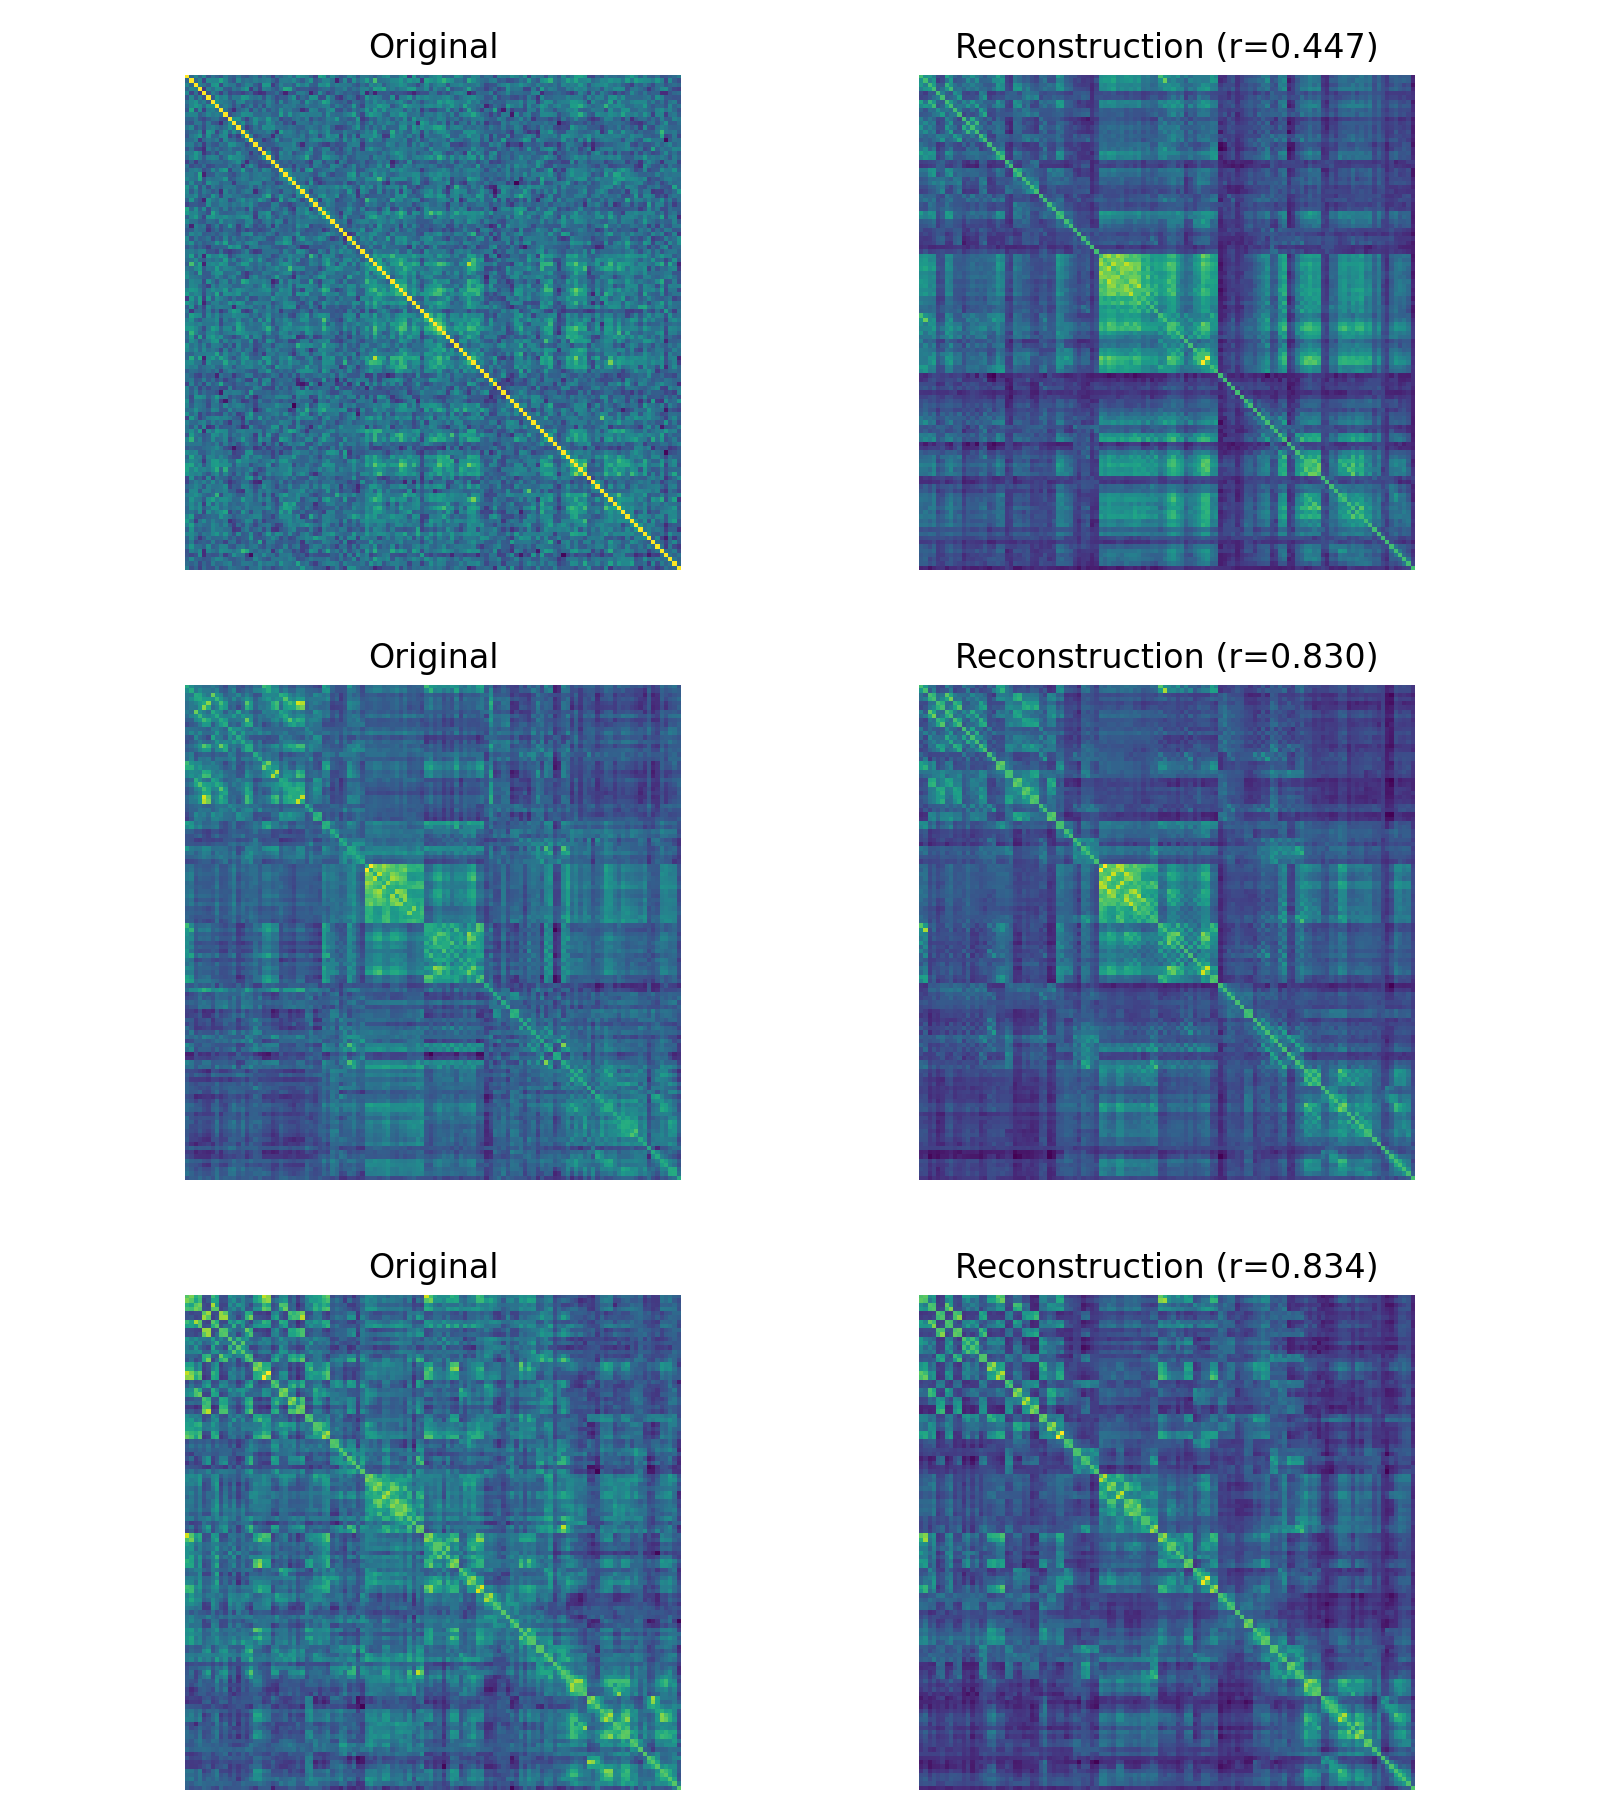
\includegraphics[width=0.85\textwidth]{06_resultados_discusion/images/vae_recons_combined.png}
    \caption{Ejemplos de reconstrucción del $\beta$-VAE para tres sujetos del conjunto trainval. Izquierda: matriz de conectividad funcional original. Derecha: reconstrucción a partir del espacio latente de 64 dimensiones. El valor $r$ indica la correlación de Pearson entre el vector original y el reconstruido para cada sujeto.}
    \label{fig:vae_recons}
\end{figure}


\section{Rendimiento del modelo principal}
\label{sec:res_principal}

El modelo principal (embeddings VAE + features T1w) se evaluó sobre el conjunto de test holdout ($n = 125$), que no fue utilizado durante el entrenamiento ni la selección de hiperparámetros. La Tabla~\ref{tab:test_metrics} presenta las métricas obtenidas.

\begin{table}[H]
\centering
\caption{Métricas de predicción de edad del modelo principal (VAE + T1w) en el conjunto de test ($n = 125$).}
\label{tab:test_metrics}
\begin{tabular}{lr}
\toprule
\textbf{Métrica} & \textbf{Valor} \\
\midrule
MAE & 5,62 años \\
RMSE & 7,20 años \\
$R^2$ & 0,411 \\
Pearson $r$ & 0,644 \\
\bottomrule
\end{tabular}
\end{table}

El modelo logra un error absoluto medio de 5,62 años, lo que significa que en promedio las predicciones se desvían menos de 6 años de la edad cronológica. El $R^2$ de 0,411 indica que el modelo logra dar cuenta de aproximadamente el 41\% de las diferencias de edad entre los sujetos del test; el 59\% restante corresponde a variabilidad que el modelo no captura (diferencias biológicas individuales, ruido de medición, etc.). La correlación de Pearson de 0,644 refleja una asociación moderada-fuerte entre edades reales y predichas. La diferencia entre MAE (5,62) y RMSE (7,20) sugiere la presencia de algunos errores de mayor magnitud en sujetos individuales.

La Figura~\ref{fig:scatter_pred} muestra el diagrama de dispersión entre la edad cronológica y la edad predicha. Los puntos se distribuyen a lo largo de la diagonal de identidad, con una dispersión mayor en los extremos del rango etario, donde la cantidad de sujetos es menor.

\begin{figure}[H]
\centering
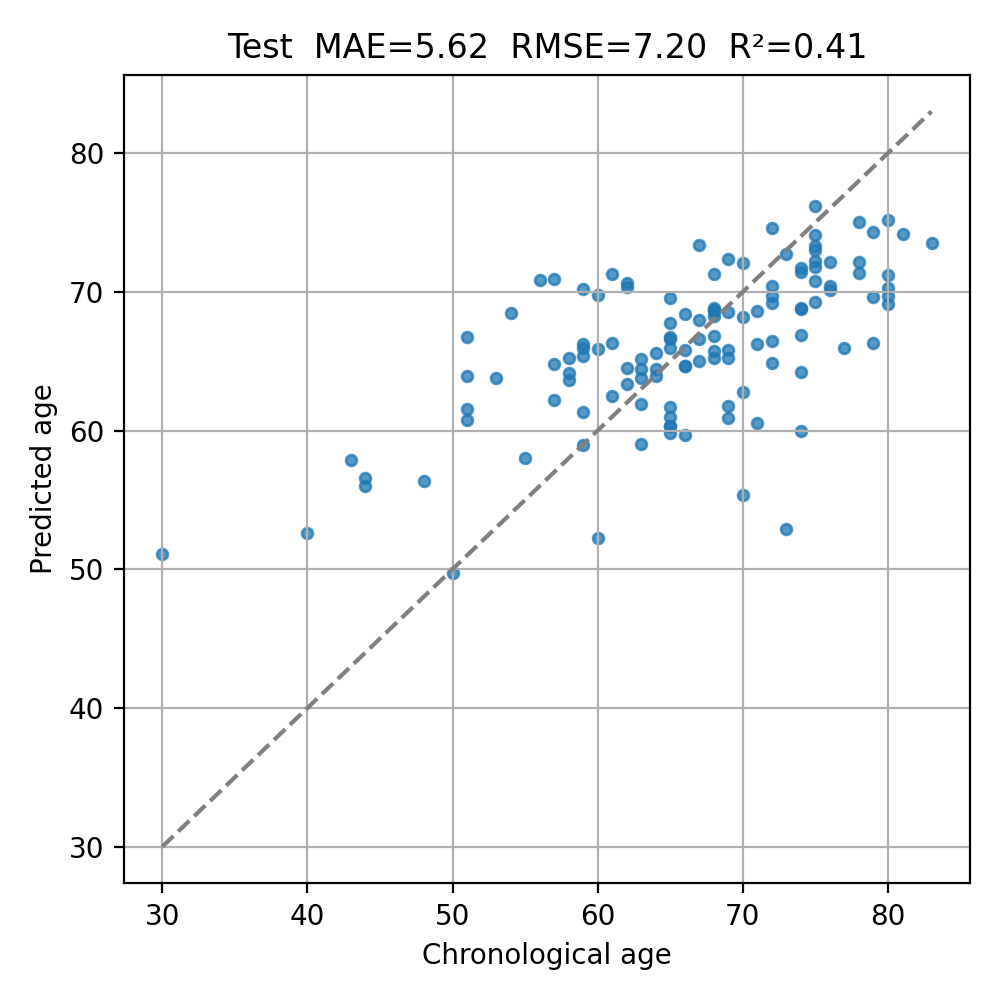
\includegraphics[width=0.7\textwidth]{06_resultados_discusion/images/xgb_scatter.png}
\caption{Edad cronológica vs.\ edad predicha por el modelo principal (VAE + T1w + XGBoost) sobre el conjunto de test ($n = 125$). La línea punteada representa la identidad (predicción perfecta).}
\label{fig:scatter_pred}
\end{figure}

XGBoost proporciona de forma directa una medida de importancia por variable (en este trabajo se usa la métrica Gain, que refleja cuánto reduce cada feature la pérdida cuando se usa en los splits de los árboles). La Figura~\ref{fig:importance} muestra las 20 más influyentes. En el modelo predominan volúmenes de materia gris en cerebelo, cíngulo, corteza frontal, pallidum, lóbulo temporal, hipocampo y tálamo; en la literatura de neuroimagen suelen reportarse cambios en estas estructuras con la edad \cite{raz2005regional, fjell2010structural}, lo que da una interpretabilidad biológica al resultado sin análisis adicionales.

\begin{figure}[H]
\centering
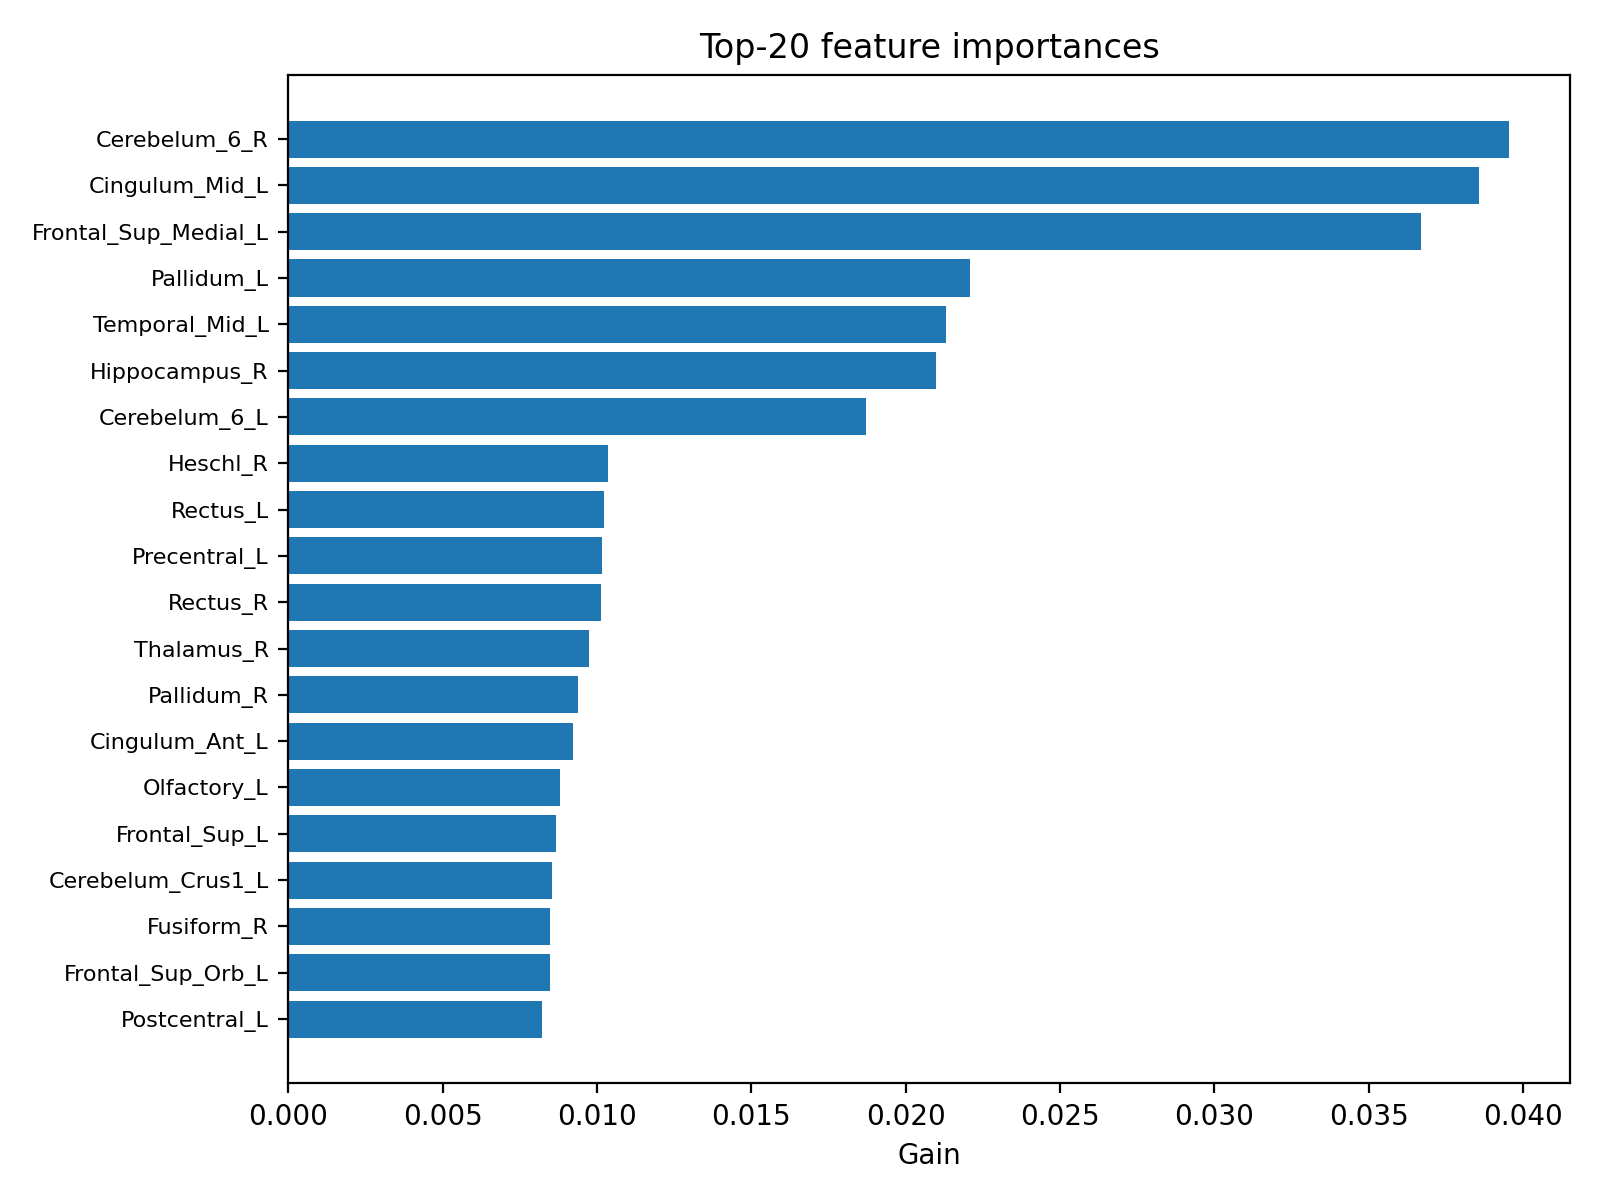
\includegraphics[width=0.85\textwidth]{06_resultados_discusion/images/xgb_importance_top20.png}
\caption{Las 20 features con mayor importancia (Gain) en el modelo XGBoost del pipeline principal. Cada feature T1w tiene la forma \texttt{t1\_XXXX}, donde el número indica el índice de la región en el atlas AAL-116 (orden canónico del atlas); en la figura se muestran los nombres anatómicos correspondientes (p.\ ej.\ Cerebellum\_6\_R, Cingulum\_Mid\_L). Las que más contribuyen coinciden con estructuras asociadas al envejecimiento cerebral en la literatura.}
\label{fig:importance}
\end{figure}


\section{Estudio de ablaciones}
\label{sec:res_ablaciones}

Para cuantificar la contribución de cada fuente de datos, se evaluaron siete configuraciones del modelo sobre el mismo conjunto de test. Todas utilizan los mismos hiperparámetros de XGBoost optimizados, variando únicamente el conjunto de features de entrada. Los resultados se presentan en la Tabla~\ref{tab:ablaciones}.

\begin{table}[H]
\centering
\caption{Resultados del estudio de ablaciones sobre el conjunto de test ($n = 125$). Se resalta en negrita la configuración con mejor MAE.}
\label{tab:ablaciones}
\begin{tabular}{lrrrr}
\toprule
\textbf{Configuración} & \textbf{MAE} & \textbf{RMSE} & \textbf{$R^2$} & \textbf{Pearson} \\
\midrule
Solo T1w & 5,89 & 7,48 & 0,366 & 0,606 \\
T1w + sexo & 5,88 & 7,44 & 0,372 & 0,612 \\
Solo VAE($\mu$) & 7,01 & 9,12 & 0,056 & 0,284 \\
VAE($\mu$) + sexo & 7,06 & 9,18 & 0,044 & 0,268 \\
\textbf{VAE($\mu$) + T1w} & \textbf{5,62} & \textbf{7,20} & \textbf{0,411} & \textbf{0,644} \\
VAE($\mu$) + T1w + sexo & 5,70 & 7,34 & 0,389 & 0,626 \\
VAE($\mu$) + T1w + sexo + diag. & 5,64 & 7,17 & 0,416 & 0,648 \\
\bottomrule
\end{tabular}
\end{table}

El resultado más relevante de las ablaciones es que la configuración VAE + T1w (MAE = 5,62) supera a T1w solo (MAE = 5,89), lo que confirma que los embeddings del VAE capturan patrones de envejecimiento en la conectividad funcional que los volúmenes de materia gris no contienen. La mejora de 0,27 años en MAE y 0,045 puntos en $R^2$ se observa de forma consistente en todas las métricas.

Sin embargo, los embeddings del VAE por sí solos resultan insuficientes: con solo features funcionales, el modelo obtiene un MAE de 7,01 y un $R^2$ de apenas 0,056. La conectividad funcional parece ser una fuente de información más ruidosa que los datos estructurales, y se beneficia sustancialmente de la complementación con T1w.

Resulta llamativo que agregar la variable sexo al modelo no mejore la predicción (MAE 5,70 vs.\ 5,62 sin sexo), a pesar de las diferencias neuroanatómicas documentadas entre sexos. Esto probablemente se deba al tamaño reducido de la muestra, que dificulta capturar efectos sutiles.

En cuanto al diagnóstico, su inclusión produce el mejor $R^2$ (0,416) pero no el mejor MAE (5,64 vs.\ 5,62). Dado que el diagnóstico está correlacionado con la edad (los pacientes con AD tienden a ser mayores), existe el riesgo de que el modelo aprenda un atajo (predecir edad alta para sujetos con AD) en lugar de capturar patrones cerebrales de envejecimiento. Por esta razón se lo excluye del modelo final.


\section{Comparación con reducción lineal (PCA)}
\label{sec:res_pca}

La elección del $\beta$-VAE como método de reducción de dimensionalidad siguió la tendencia predominante en la literatura de neuroimagen computacional, donde los autoencoders variacionales se han consolidado como herramientas estándar para aprender representaciones latentes de datos cerebrales de alta dimensionalidad \cite{higgins2017beta, dufumier2024multi}. No obstante, una vez construido y optimizado el pipeline completo, resulta pertinente validar si la complejidad adicional del VAE respecto a un método lineal clásico se traduce en una mejora de rendimiento. Para ello, se comparó con PCA utilizando 64 componentes (la misma dimensionalidad que el espacio latente del VAE).

Ambos métodos se combinaron con features T1w y se evaluaron con un modelo XGBoost utilizando los hiperparámetros optimizados por Optuna para la configuración VAE + T1w. Dado que ambas configuraciones producen vectores de 180 dimensiones (64 de la reducción + 116 de T1w), estos hiperparámetros son razonables para ambos métodos. Los resultados se presentan en la Tabla~\ref{tab:pca_vs_vae}.

\begin{table}[H]
\centering
\caption{Comparación entre PCA y VAE como método de reducción de dimensionalidad para las matrices de conectividad funcional. Ambos reducen a 64 dimensiones y se combinan con T1w.}
\label{tab:pca_vs_vae}
\begin{tabular}{lrrrr}
\toprule
\textbf{Método} & \textbf{MAE} & \textbf{RMSE} & \textbf{$R^2$} & \textbf{Pearson} \\
\midrule
PCA (64 componentes) & 5,61 & 7,08 & 0,431 & 0,661 \\
$\beta$-VAE (64 dimensiones latentes) & 5,62 & 7,20 & 0,411 & 0,644 \\
\bottomrule
\end{tabular}
\end{table}

Contrariamente a lo esperado, PCA y el $\beta$-VAE alcanzan un rendimiento prácticamente equivalente: la diferencia en MAE es de apenas 0,01 años y en $R^2$ de 0,020, ambas dentro del margen de variabilidad del conjunto de test ($n = 125$). PCA incluso obtiene valores numéricamente superiores en todas las métricas, aunque las diferencias no son estadísticamente significativas. Cabe notar que los hiperparámetros de XGBoost fueron optimizados por Optuna específicamente para la configuración VAE + T1w; si PCA contara con su propia optimización independiente, su rendimiento podría ser incluso superior. En este sentido, el hecho de que PCA iguale o supere al VAE utilizando hiperparámetros ajustados para el VAE refuerza la robustez de este hallazgo.

Este resultado tiene varias implicaciones. Primero, sugiere que la información relevante para la predicción de edad en las matrices de conectividad funcional es capturada en buena medida por las componentes principales, es decir, por las direcciones de máxima varianza. Este hallazgo es consistente con Monti et al. \cite{monti2020interpretable}, quienes demostraron que un enfoque en dos etapas (reducción lineal de dimensionalidad de matrices de conectividad funcional seguida de regresión) permite predecir la edad cerebral de forma generalizable a través de múltiples cohortes. Cabe notar que en ese trabajo, PCA sin restricciones fue el método de menor rendimiento entre los evaluados, y extensiones con restricciones de no-negatividad y ortogonalidad obtuvieron mejores resultados; sin embargo, en el presente trabajo el uso de un regresor no lineal (XGBoost) en la segunda etapa podría compensar la simplicidad de PCA en la primera. Segundo, indica que un regresor suficientemente potente como XGBoost puede extraer patrones no lineales incluso a partir de features linealmente proyectados, lo que reduce la ventaja de una representación no lineal como la del VAE. Tercero, la convergencia de resultados entre PCA y VAE es consistente con el hallazgo de la Sección~\ref{sec:res_regresores}, donde tres familias de regresores diferentes también alcanzan rendimientos equivalentes: una vez que los datos se comprimen a una dimensionalidad adecuada, el rendimiento depende más de la información contenida en los datos que del método de representación o del regresor. More et al. \cite{more2023brain}, en su comparación sistemática de 128 workflows de predicción de brain age, observaron que tanto la representación de los datos como el algoritmo de aprendizaje automático afectan el rendimiento, y que las features a nivel de vóxel combinadas con PCA y algoritmos no lineales se encuentran entre las configuraciones de mejor desempeño.

No obstante, este resultado debe interpretarse con cautela. La optimización de la arquitectura del VAE exploró únicamente 70 configuraciones (trials de Optuna) dentro de un espacio de búsqueda combinatorio vasto que incluye la dimensión latente, el número y tamaño de capas ocultas, el valor de $\beta$, la tasa de dropout, el learning rate, las épocas de warmup y el tipo de embedding. Es plausible que configuraciones no exploradas del VAE logren un rendimiento superior al de PCA, particularmente con cohortes mayores donde los métodos no lineales suelen beneficiarse de la mayor cantidad de datos de entrenamiento.

Además, el $\beta$-VAE ofrece ventajas cualitativas que PCA no posee y que justifican su inclusión en el pipeline. Como modelo generativo, permite la reconstrucción y visualización de las matrices FC originales a partir del espacio latente, proporcionando una herramienta de verificación de la calidad de las representaciones aprendidas. Asimismo, la optimización downstream de sus hiperparámetros orienta la representación hacia la tarea de predicción de edad, una capacidad que PCA no puede ofrecer (carece de hiperparámetros ajustables más allá del número de componentes).


\section{Comparación con features crudos de FC (sin reducción)}
\label{sec:res_raw_fc}

Para evaluar si la reducción de dimensionalidad del VAE es realmente necesaria, o si XGBoost puede manejar directamente los features de alta dimensionalidad, se comparó el pipeline VAE + T1w con una variante que utiliza los 6670 valores crudos del triángulo superior de la matriz FC concatenados con los 116 features T1w (6786 features totales). Para garantizar una comparación justa, los hiperparámetros de XGBoost se optimizaron de forma independiente con Optuna (50 trials, 5-fold CV) para cada configuración, en lugar de reutilizar los parámetros optimizados para una de las dos. Los resultados se presentan en la Tabla~\ref{tab:raw_fc_vs_vae}.

\begin{table}[H]
\centering
\caption{Comparación entre el uso directo de los features crudos de FC y la reducción vía $\beta$-VAE, ambos combinados con T1w. Cada configuración tiene hiperparámetros de XGBoost optimizados independientemente con Optuna.}
\label{tab:raw_fc_vs_vae}
\begin{tabular}{lrrrrr}
\toprule
\textbf{Método} & \textbf{Features} & \textbf{MAE} & \textbf{RMSE} & \textbf{$R^2$} & \textbf{Pearson} \\
\midrule
FC crudo + T1w & 6786 & 6,00 & 7,55 & 0,354 & 0,601 \\
$\beta$-VAE + T1w & 180 & 5,62 & 7,20 & 0,411 & 0,644 \\
\midrule
\textbf{Ventaja del VAE} & \textbf{$-$97,3\%} & \textbf{$-$0,38} & \textbf{$-$0,35} & \textbf{+0,057} & \textbf{+0,043} \\
\bottomrule
\end{tabular}
\end{table}

Aun con hiperparámetros optimizados específicamente para la entrada de alta dimensionalidad, el VAE supera a los features crudos en todas las métricas: la mejora en MAE es de 0,38 años y en $R^2$ de 16\% relativo (de 0,354 a 0,411). La correlación de Pearson también es superior (0,644 vs.\ 0,601). Esto confirma que la ventaja del VAE no se debe a una elección desfavorable de hiperparámetros, sino a la calidad de las representaciones aprendidas.

El análisis de los hiperparámetros optimizados por Optuna para cada configuración es revelador. Para el pipeline VAE + T1w (180 features), Optuna seleccionó árboles profundos (\texttt{max\_depth}~$= 6$) que observan casi todas las features por árbol. En cambio, para los features crudos (6786), Optuna seleccionó árboles poco profundos (\texttt{max\_depth}~$= 3$) donde cada árbol observa solo el 10\% de los features, con mayor regularización y un peso mínimo por hoja diez veces superior. Esto indica que el regresor necesita una regularización agresiva para manejar la alta dimensionalidad, descartando implícitamente la mayoría de los features en cada paso. La compresión del VAE realiza esta selección de información de forma más sistemática y efectiva, produciendo representaciones densas donde todas las dimensiones son informativas.


\section{Comparación de regresores}
\label{sec:res_regresores}

Para evaluar si el rendimiento del pipeline depende del regresor específico o de la representación aprendida, se compararon tres familias de modelos: regresión lineal regularizada (Ridge), regresión por vectores de soporte con kernel RBF (SVR) y gradient boosting (XGBoost). Los tres regresores recibieron exactamente las mismas features de entrada (embeddings VAE $\mu$ + T1w, 180 dimensiones) y se evaluaron sobre los mismos conjuntos de validación cruzada y test.

Para garantizar una comparación justa, los hiperparámetros de cada modelo se optimizaron con Optuna mediante 100 trials sobre los mismos 5 folds de validación cruzada empleados en el pipeline principal. Los resultados se resumen en la Tabla~\ref{tab:model_comparison}.

\begin{table}[H]
\centering
\caption{Comparación de regresores, todos optimizados con Optuna (100 trials, 5-fold CV). Se reportan el MAE de validación cruzada (CV MAE) y las métricas sobre el conjunto de test ($n = 125$).}
\label{tab:model_comparison}
\begin{tabular}{lrrrrr}
\toprule
\textbf{Modelo} & \textbf{CV MAE} & \textbf{MAE} & \textbf{RMSE} & \textbf{$R^2$} & \textbf{Pearson} \\
\midrule
Ridge          & 6,54 & 5,75 & 7,25 & 0,403 & 0,639 \\
SVR (RBF)      & 6,22 & 5,65 & 7,02 & 0,441 & 0,664 \\
XGBoost        & 6,36 & 5,62 & 7,20 & 0,411 & 0,644 \\
\bottomrule
\end{tabular}
\end{table}

Los tres regresores alcanzan un rendimiento muy similar: la diferencia máxima en MAE de test es de apenas 0,13 años entre Ridge y XGBoost, y de 0,03 años entre SVR y XGBoost. En validación cruzada, SVR obtiene el menor error promedio (6,22), mientras que XGBoost presenta el menor MAE de test (5,62). Estas diferencias se encuentran dentro del margen de variabilidad esperado para un conjunto de test de 125 sujetos.

La convergencia de rendimiento entre tres familias de modelos fundamentalmente distintas (lineal, kernel y ensemble de árboles) indica que el factor determinante de la predicción no es el regresor sino la calidad de las representaciones construidas en la etapa de extracción de features. Se mantiene XGBoost en el pipeline principal por una razón práctica de interpretación: los árboles de decisión permiten obtener, del propio entrenamiento, una medida de importancia por variable (Gain), sin necesidad de análisis adicionales. Con Ridge solo se tienen coeficientes de una combinación lineal, y con SVR la interpretación de la contribución individual de cada feature resulta considerablemente más compleja. Con XGBoost basta con consultar las importancias nativas del modelo para discutir qué regiones o dimensiones latentes son más relevantes (Figura~\ref{fig:importance}).


\section{Evaluación del entrenamiento exclusivo en controles sanos}
\label{sec:res_cn_only}

Se evaluó una estrategia alternativa en la que tanto el VAE como el XGBoost se entrenan exclusivamente sobre los sujetos cognitivamente normales (CN) del conjunto trainval ($n_{\text{CN}} = 473$), con el objetivo de aprender el patrón de envejecimiento normal y medir la \textit{brain age gap} en poblaciones clínicas.

Dado que el modelo fue entrenado únicamente con sujetos CN, todos los pacientes con AD y FTD constituyen datos no vistos durante el entrenamiento. Esto permite utilizar la totalidad de ambos grupos clínicos para la evaluación, no solamente los sujetos del conjunto de test del pipeline principal. En cambio, para los sujetos CN se emplean únicamente los 53 del conjunto de test, ya que los restantes 473 fueron utilizados para entrenar el modelo. Los resultados por grupo diagnóstico se presentan en la Tabla~\ref{tab:cn_only}.

\begin{table}[H]
\centering
\caption{Rendimiento del modelo entrenado exclusivamente en controles sanos. CN se evalúa sobre los 53 sujetos del conjunto de test; AD y FTD se evalúan sobre la totalidad de sus respectivas cohortes, ya que ninguno fue utilizado durante el entrenamiento.}
\label{tab:cn_only}
\begin{tabular}{lrrrrrr}
\toprule
\textbf{Grupo} & \textbf{$n$} & \textbf{MAE} & \textbf{RMSE} & \textbf{$R^2$} & \textbf{Pearson} & \textbf{Gap} \\
\midrule
CN  & 53  & 6,03 & 7,33 & 0,504  & 0,717 & $-$0,42 \\
AD  & 422 & 7,36 & 9,19 & $-$0,170 & 0,129 & $-$1,86 \\
FTD & 297 & 6,93 & 8,90 & $-$0,153 & 0,165 & $+$1,84 \\
\bottomrule
\end{tabular}
\end{table}

El modelo CN-only obtiene un MAE de 6,03 años en los 53 sujetos CN del test, superior al MAE de 5,62 del modelo mixto. Esto indica que, con 473 sujetos sanos, el modelo no captura los patrones del envejecimiento normal con precisión suficiente. En ambas poblaciones clínicas, los valores de $R^2$ son negativos, lo que indica predicciones peores que la media, y las correlaciones de Pearson son débiles ($< 0{,}2$).

La brain age gap media en FTD fue de $+1{,}84$ años, es decir, el modelo predice que los pacientes con demencia frontotemporal tienen cerebros \textit{más viejos} que su edad cronológica. Esta dirección coincide con la esperada en la literatura, donde el envejecimiento acelerado es un marcador de neurodegeneración \cite{franke2010estimating}. Sin embargo, en AD la gap fue de $-1{,}86$ años (dirección opuesta), lo que contradice la evidencia publicada. La divergencia entre ambos grupos clínicos sugiere que, con 473 sujetos de entrenamiento, el modelo captura una señal débil e inconsistente, insuficiente para funcionar como biomarcador.

El rendimiento inferior respecto al modelo mixto podría atribuirse a dos factores: (i)~la reducción del conjunto de entrenamiento (473 sujetos frente a 1120), y (ii)~la reutilización de hiperparámetros optimizados para la cohorte completa, que pueden no ser óptimos para la sub-cohorte CN. Para descartar el factor~(ii), se realizó un experimento adicional con optimización Optuna dedicada para los datos CN (50 trials para el $\beta$-VAE y 100 para XGBoost). Los resultados fueron similares: MAE de 6,29 en CN, gaps de $-2{,}21$ en AD y $+1{,}71$ en FTD, confirmando que la limitación principal es el tamaño de la muestra y no la configuración de hiperparámetros. Esto es consistente con la literatura, donde los estudios de brain age basados exclusivamente en sujetos sanos suelen requerir cohortes del orden de $N > 2000$ para obtener MAE competitivos y gaps clínicamente significativos \cite{franke2010estimating}.

Por estas razones, se descartó este enfoque en favor del entrenamiento mixto (CN + AD + FTD), que obtiene un rendimiento más robusto y generalizable (MAE = 5,62) y aprovecha la totalidad de la muestra disponible.

\subsection{Modelo CN-only con variables demográficas}
\label{sec:res_cn_demo}

De forma exploratoria, se evaluó si la inclusión de variables demográficas (educación y sitio) podría mejorar el modelo CN-only. Para este experimento se utilizaron únicamente los 337 sujetos CN que disponen de datos demográficos completos, lo que constituye una reducción adicional respecto a los 473 CN del experimento anterior. La Tabla~\ref{tab:cn_demo} compara los resultados del modelo CN-only con y sin variables demográficas.

\begin{table}[H]
\centering
\caption{Modelo CN-only con y sin variables demográficas. Ambos modelos fueron entrenados exclusivamente con los 337 CN que disponen de datos demográficos (a diferencia de la Tabla~\ref{tab:cn_only}, que utiliza los 473 CN totales); la diferencia de tamaño y composición del conjunto de entrenamiento explica las diferencias numéricas entre ambas tablas. Los grupos clínicos (AD, FTD) incluyen únicamente los sujetos con datos demográficos disponibles.}
\label{tab:cn_demo}
\begin{tabular}{llrrrr}
\toprule
\textbf{Modelo} & \textbf{Grupo} & \textbf{$n$} & \textbf{MAE} & \textbf{$R^2$} & \textbf{Gap} \\
\midrule
\multirow{3}{*}{CN baseline} & CN (test) & 53 & 6,09 & 0,487 & $-$0,07 \\
                             & AD       & 422 & 6,97 & $-$0,113 & $+$0,21 \\
                             & FTD      & 297 & 7,42 & $-$0,335 & $+$4,01 \\
\midrule
\multirow{3}{*}{CN + edu + sitio} & CN (test) & 37 & 5,51 & 0,569 & $+$0,41 \\
                                  & AD       & 348 & 6,41 & 0,054 & $+$0,70 \\
                                  & FTD      & 211 & 6,49 & $-$0,071 & $+$4,11 \\
\bottomrule
\end{tabular}
\end{table}

La inclusión de educación y sitio mejora el MAE en CN de 6,09 a 5,51 años y, de forma relevante, las gaps en ambos grupos clínicos son consistentemente positivas: $+0{,}70$ en AD y $+4{,}11$ en FTD. Esta dirección (cerebro más viejo de lo esperado) es la esperada en la neurodegeneración. En contraste, el modelo CN baseline sin demográficos obtiene una gap cercana a cero en AD ($+0{,}21$), lo que dificulta la interpretación clínica. La Figura~\ref{fig:cn_demo_importance} muestra la importancia de las features en el modelo CN + educación + sitio: la variable \texttt{education} se posiciona entre las más relevantes, lo que sugiere que la información socioeconómica aporta señal complementaria a las features de neuroimagen.

\begin{figure}[H]
\centering
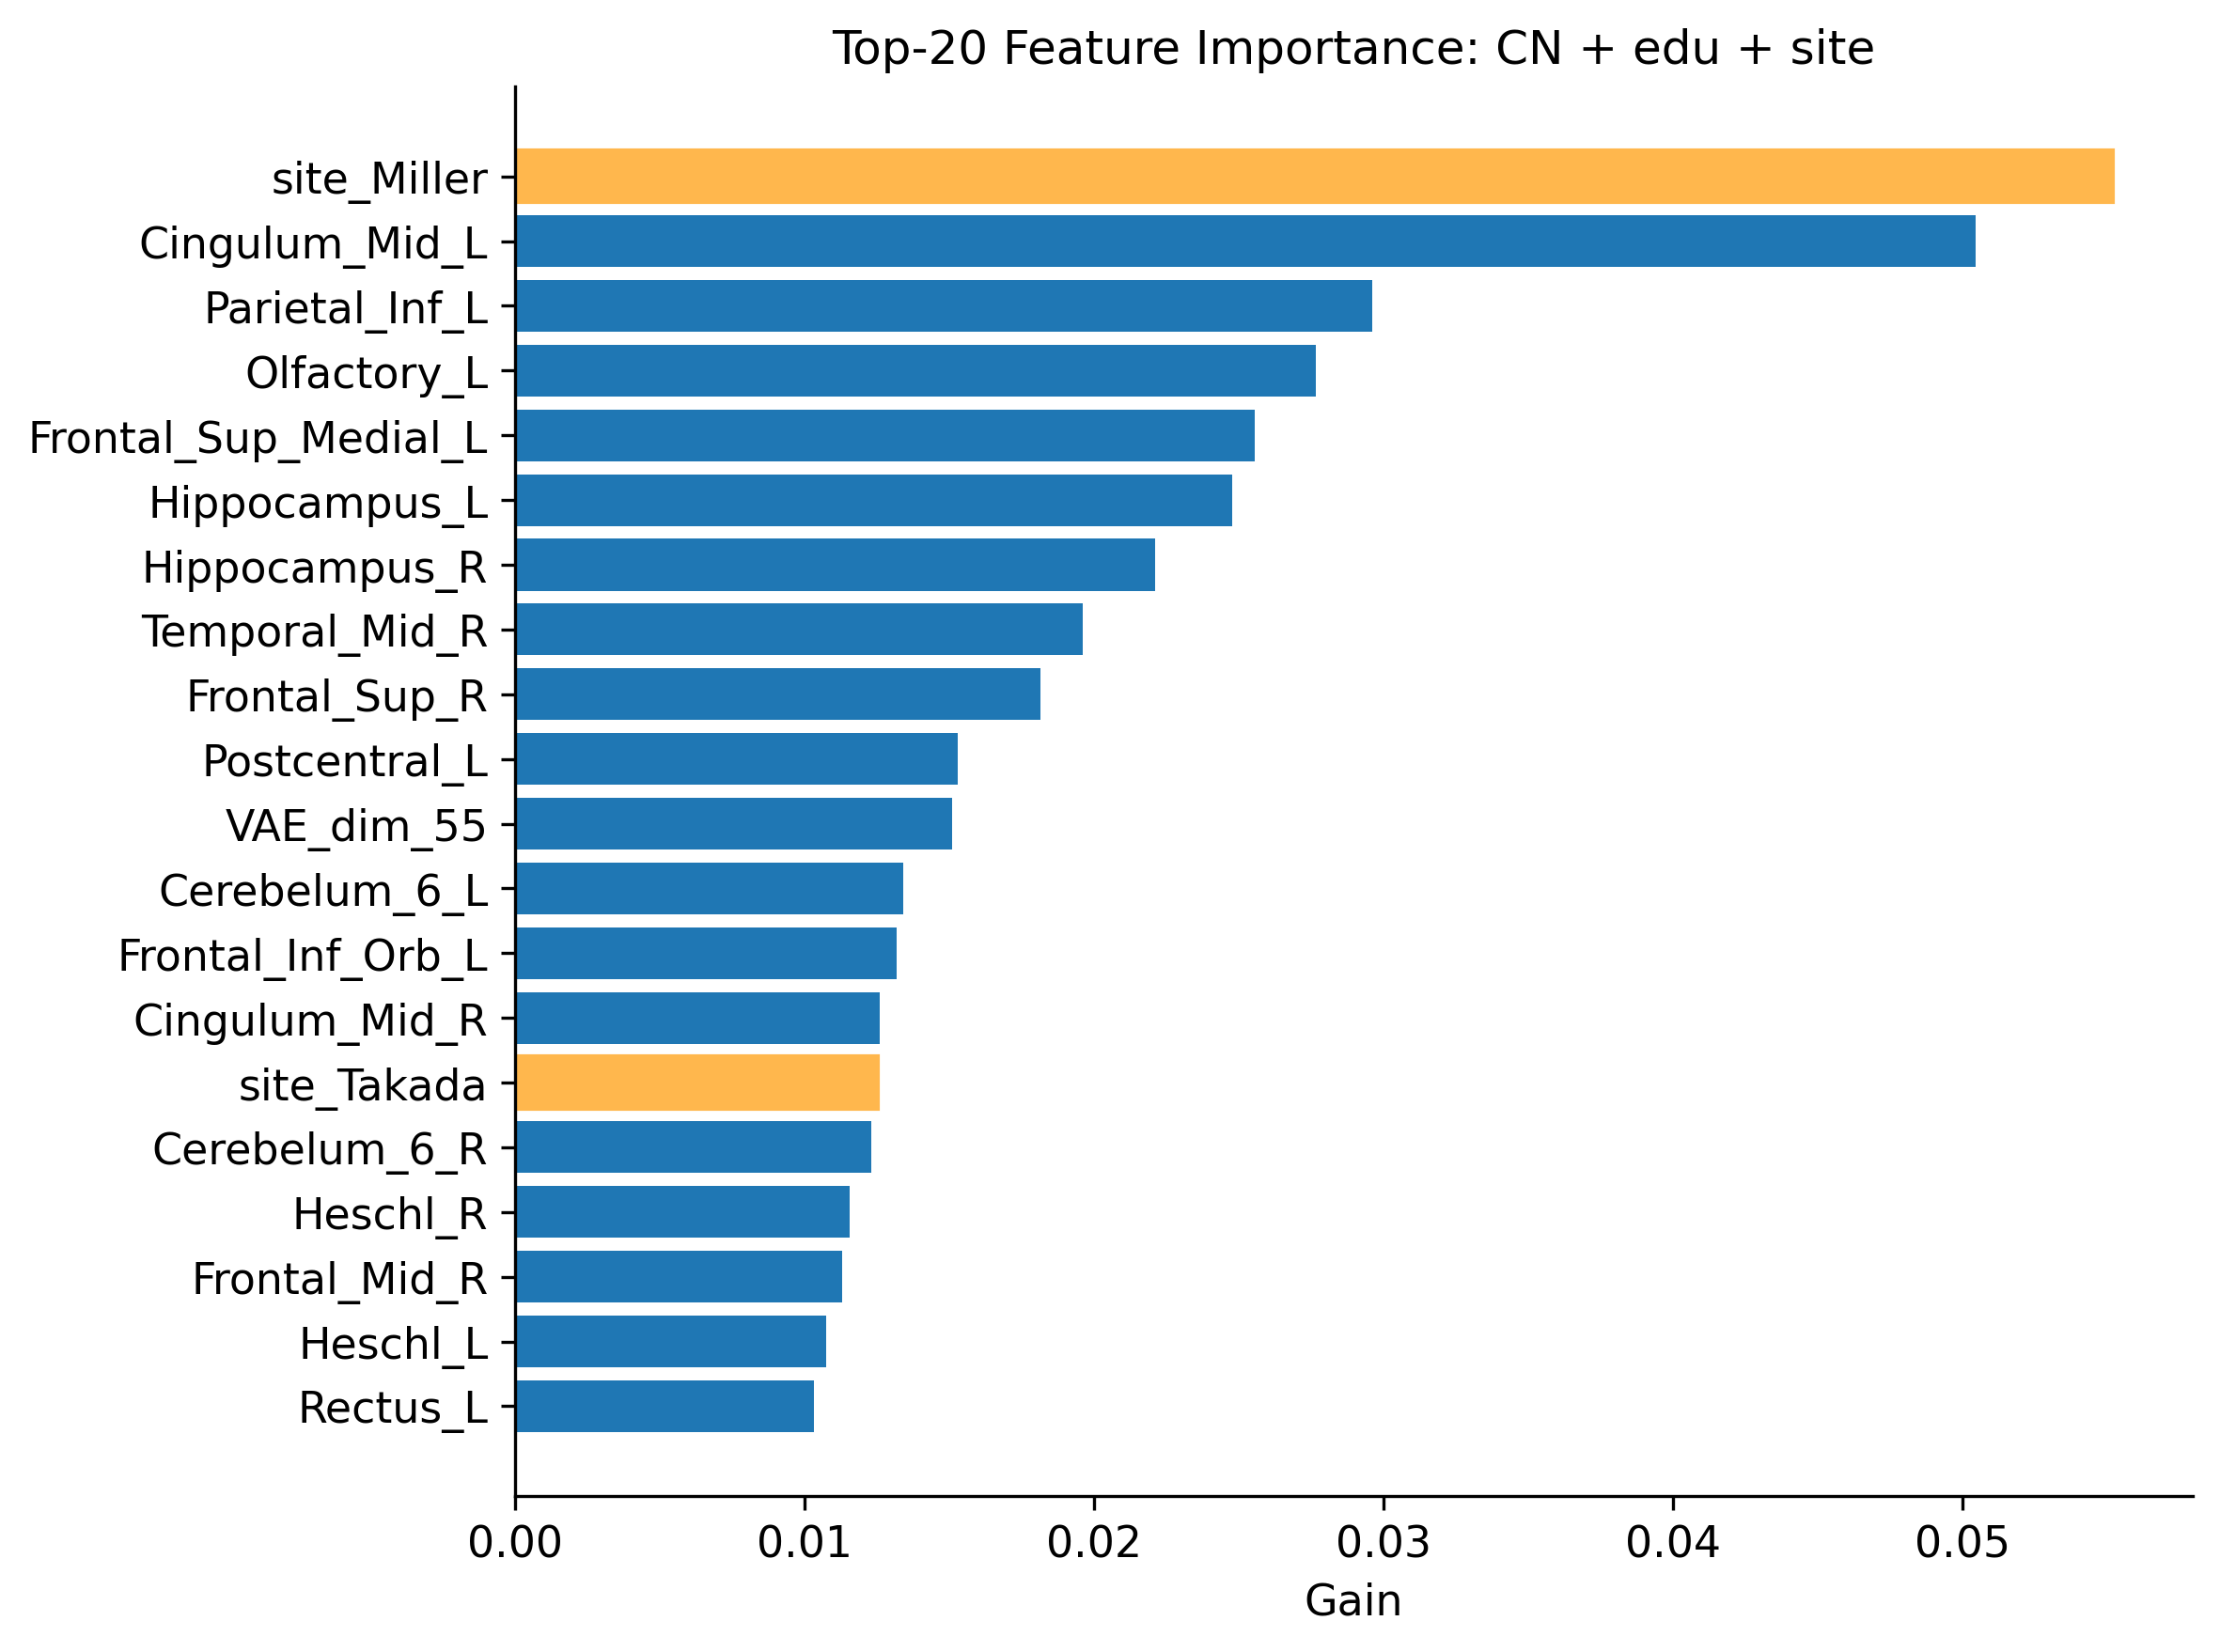
\includegraphics[width=0.7\textwidth]{06_resultados_discusion/images/cn_demo_importance.png}
\caption{Top 20 features por importancia (XGBoost \textit{gain}) en el modelo CN-only entrenado con educación y sitio como features adicionales. Las features VAE\_dim\_$N$ representan dimensiones latentes del $\beta$-VAE (patrones de conectividad funcional) y no corresponden a una región cerebral individual.}
\label{fig:cn_demo_importance}
\end{figure}

Estos resultados son exploratorios y deben interpretarse con cautela dado el reducido tamaño de la muestra de entrenamiento ($n = 337$ CN) y de test ($n = 37$ CN). No obstante, la consistencia de las gaps positivas en ambos grupos clínicos sugiere que, con una cohorte CN más amplia y datos demográficos completos, la inclusión de estas variables podría contribuir a mejorar la viabilidad del pipeline como biomarcador.

\section{Impacto de variables demográficas}
\label{sec:res_demograficas}

Dada la heterogeneidad socioeconómica y multicéntrica de la cohorte RedLaT, se analizó el impacto de variables demográficas sobre la predicción de edad cerebral. Las variables exploradas fueron los años de educación formal (\texttt{cog\_ed}, disponible para el 74,9\% de la cohorte), el sitio de adquisición (75,6\%) y la marca del escáner MRI (74,0\%). El análisis se realizó en dos direcciones complementarias: (i)~correlación entre las variables demográficas y la brain age gap del modelo principal, y (ii)~inclusión de dichas variables como features adicionales en el modelo de predicción.

\subsection{Brain age gap y años de educación}
\label{sec:res_gap_educacion}

Antes de evaluar si las variables demográficas mejoran la predicción del modelo (lo cual se analiza en la Sección~\ref{sec:res_demo_ablacion}), es relevante entender si estas variables se \emph{asocian} con los errores que el modelo ya comete. Para ello se utiliza la brain age gap, es decir, la diferencia entre la edad que el modelo predice para el cerebro de una persona y su edad cronológica real. Por ejemplo, si el modelo dice que el cerebro de una persona de 60 años ``parece'' de 65, su gap es de $+5$ años; si parece de 55, su gap es de $-5$ años. Una gap positiva indica que el modelo percibe un cerebro más envejecido de lo esperado, y una negativa lo contrario.

La pregunta concreta de esta sección es: ¿las personas con más años de educación tienden a tener gaps más positivas o más negativas? Y lo mismo para cada grupo diagnóstico por separado. La respuesta no nos dice si agregar educación al modelo mejora su precisión (eso se responde después), sino si la educación está relacionada con que el modelo sobreestime o subestime la edad cerebral, lo cual tiene implicaciones para entender los factores que modulan el envejecimiento.

Para cada sujeto se calculó la gap a partir de las predicciones del modelo principal. En el caso de los sujetos del conjunto trainval, las predicciones se obtuvieron mediante validación cruzada con 5 folds para evitar el sobreajuste. La Tabla~\ref{tab:gap_education} resume las correlaciones (Pearson $r$ y Spearman $\rho$; véase la Sección~\ref{sec:analisis_exploratorio} del Capítulo~\ref{chapter:datos_cohorte} para una explicación detallada de estos coeficientes) entre la gap y los años de educación, estratificadas por diagnóstico.

\begin{table}[H]
\centering
\caption{Correlación entre brain age gap y años de educación, por grupo diagnóstico.}
\label{tab:gap_education}
\begin{tabular}{lrrrrr}
\toprule
\textbf{Grupo} & \textbf{$n$} & \textbf{Pearson $r$} & \textbf{$p$} & \textbf{Spearman $\rho$} & \textbf{$p$} \\
\midrule
CN  & 374 & $-$0,067 & 0,193  & $-$0,091 & 0,079 \\
AD  & 348 & $+$0,165 & 0,002  & $+$0,157 & 0,003 \\
FTD & 211 & $+$0,002 & 0,980  & $-$0,025 & 0,716 \\
Todos & 933 & $+$0,070 & 0,033  & $+$0,038 & 0,251 \\
\bottomrule
\end{tabular}
\end{table}

En controles sanos, la correlación es débil y no significativa ($r = -0{,}067$, $p = 0{,}19$), aunque la dirección negativa sugiere una tendencia sutil en la que mayor educación se asocia con un cerebro predicho como ligeramente más joven. Este patrón es consistente con la hipótesis de reserva cognitiva, que propone que la educación y la estimulación intelectual acumulada a lo largo de la vida fortalecen las redes neuronales, permitiendo al cerebro tolerar mayor daño antes de manifestar síntomas clínicos; en términos del modelo, esto se traduciría en un cerebro que ``aparenta'' ser más joven de lo esperado para su edad cronológica.

En pacientes con AD, la correlación es positiva y estadísticamente significativa ($r = +0{,}165$, $p = 0{,}002$): mayor educación se asocia con una gap más positiva (cerebro predicho como más viejo). Este hallazgo, aparentemente paradójico, puede explicarse por la misma reserva cognitiva: los pacientes con mayor educación mantienen el funcionamiento cognitivo durante más tiempo a pesar de la neurodegeneración, por lo que acceden al diagnóstico en estadios más avanzados de la enfermedad, cuando la atrofia cerebral es más pronunciada y el modelo detecta un cerebro significativamente más envejecido. En FTD no se observa correlación ($r \approx 0$).

La Figura~\ref{fig:demo_gap_vs_education} ilustra la relación entre la brain age gap y los años de educación para cada grupo diagnóstico.

\begin{figure}[H]
\centering
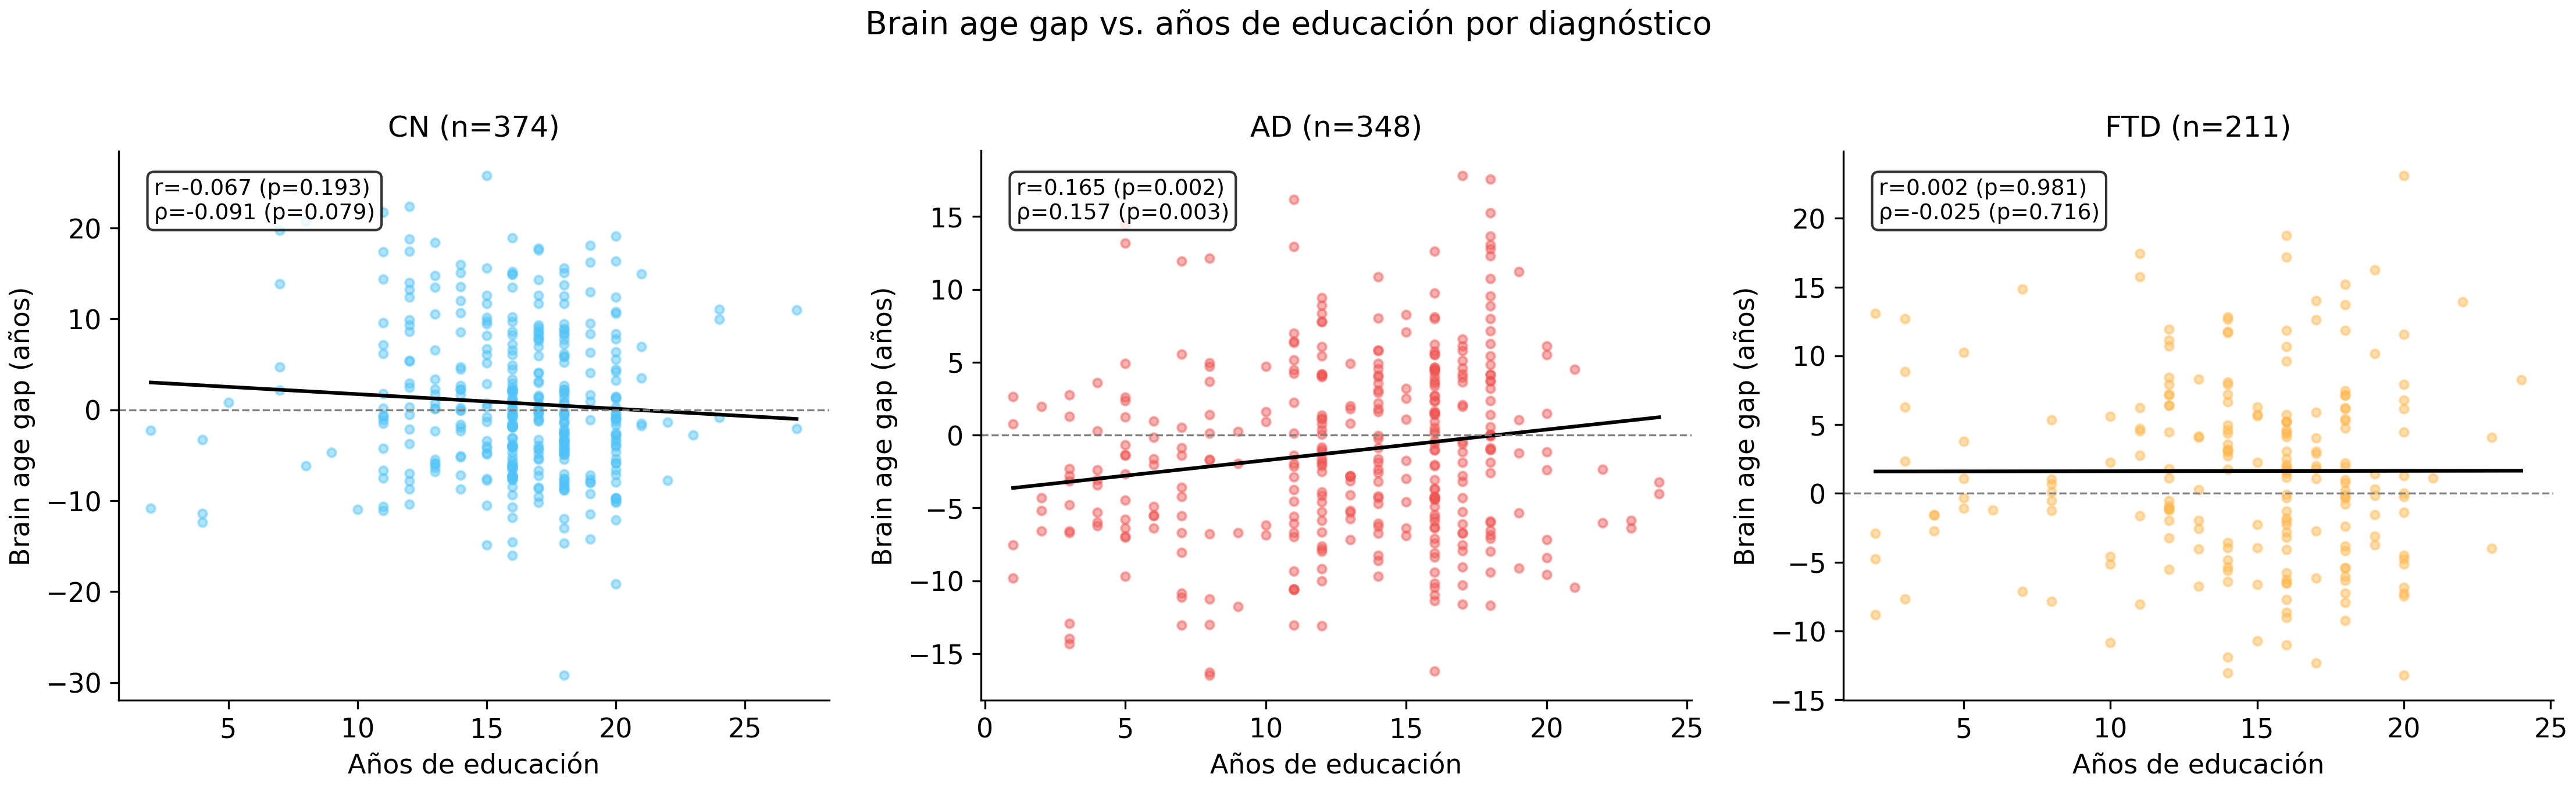
\includegraphics[width=0.95\textwidth]{06_resultados_discusion/images/demo_gap_vs_education.png}
\caption{Brain age gap vs.\ años de educación por grupo diagnóstico. La recta indica la tendencia lineal. En AD se observa una correlación positiva significativa; en CN una tendencia negativa débil; en FTD ausencia de correlación.}
\label{fig:demo_gap_vs_education}
\end{figure}

\subsection{Brain age gap y sitio de adquisición}
\label{sec:res_gap_sitio}

Con el fin de evaluar si los sujetos de distintos sitios de adquisición presentan brain age gaps distintas entre sí, o si las diferencias observadas podrían deberse al azar, se utilizó un análisis de varianza (\textbf{ANOVA}), una prueba estadística diseñada para comparar los promedios de tres o más grupos a la vez. La lógica de ANOVA es la siguiente: si todos los grupos tuvieran realmente la misma gap promedio, las diferencias que veríamos entre ellos serían pequeñas y comparables a la variación que existe dentro de cada grupo; en cambio, si las diferencias entre grupos son mucho mayores que la variación interna, ANOVA lo detecta con un valor $p$ bajo ($p < 0{,}05$), indicando que las diferencias son reales. En este caso, ANOVA arrojó $F = 8{,}67$ con $p < 0{,}001$, lo que confirma que el sitio de adquisición sí tiene un efecto significativo sobre la brain age gap.

La Tabla~\ref{tab:gap_site} presenta las estadísticas descriptivas de la gap por sitio para los sitios con al menos 20 sujetos. La columna ``gap media'' es el promedio de la brain age gap (edad predicha $-$ edad real) de los sujetos de cada sitio: por ejemplo, si un sitio tiene una gap media de $+4{,}30$ años, significa que en promedio el modelo predice que los cerebros de las personas de ese centro son 4,3 años más viejos de lo que realmente son. Un valor negativo indica lo contrario. La columna ``DE'' es la desviación estándar, que mide cuánta variación hay entre los sujetos de un mismo sitio.

\begin{table}[H]
\centering
\caption{Brain age gap por sitio de adquisición (sitios con $n \geq 20$). Se observan diferencias significativas entre sitios (ANOVA $p < 0{,}001$).}
\label{tab:gap_site}
\begin{tabular}{lrrr}
\toprule
\textbf{Sitio} & \textbf{$n$} & \textbf{Gap media} & \textbf{DE} \\
\midrule
Bruno       & 48  & $+$4,30 & 8,80 \\
Takada      & 89  & $+$2,82 & 9,20 \\
Slachevsky  & 93  & $+$1,15 & 7,89 \\
Matallana   & 135 & $+$0,92 & 6,21 \\
Miller      & 400 & $-$0,20 & 6,69 \\
Behrens     & 60  & $-$1,05 & 6,80 \\
Lopera      & 88  & $-$3,64 & 6,04 \\
\bottomrule
\end{tabular}
\end{table}

La Figura~\ref{fig:demo_gap_by_site} muestra la distribución de la brain age gap por sitio de adquisición.

\begin{figure}[H]
\centering
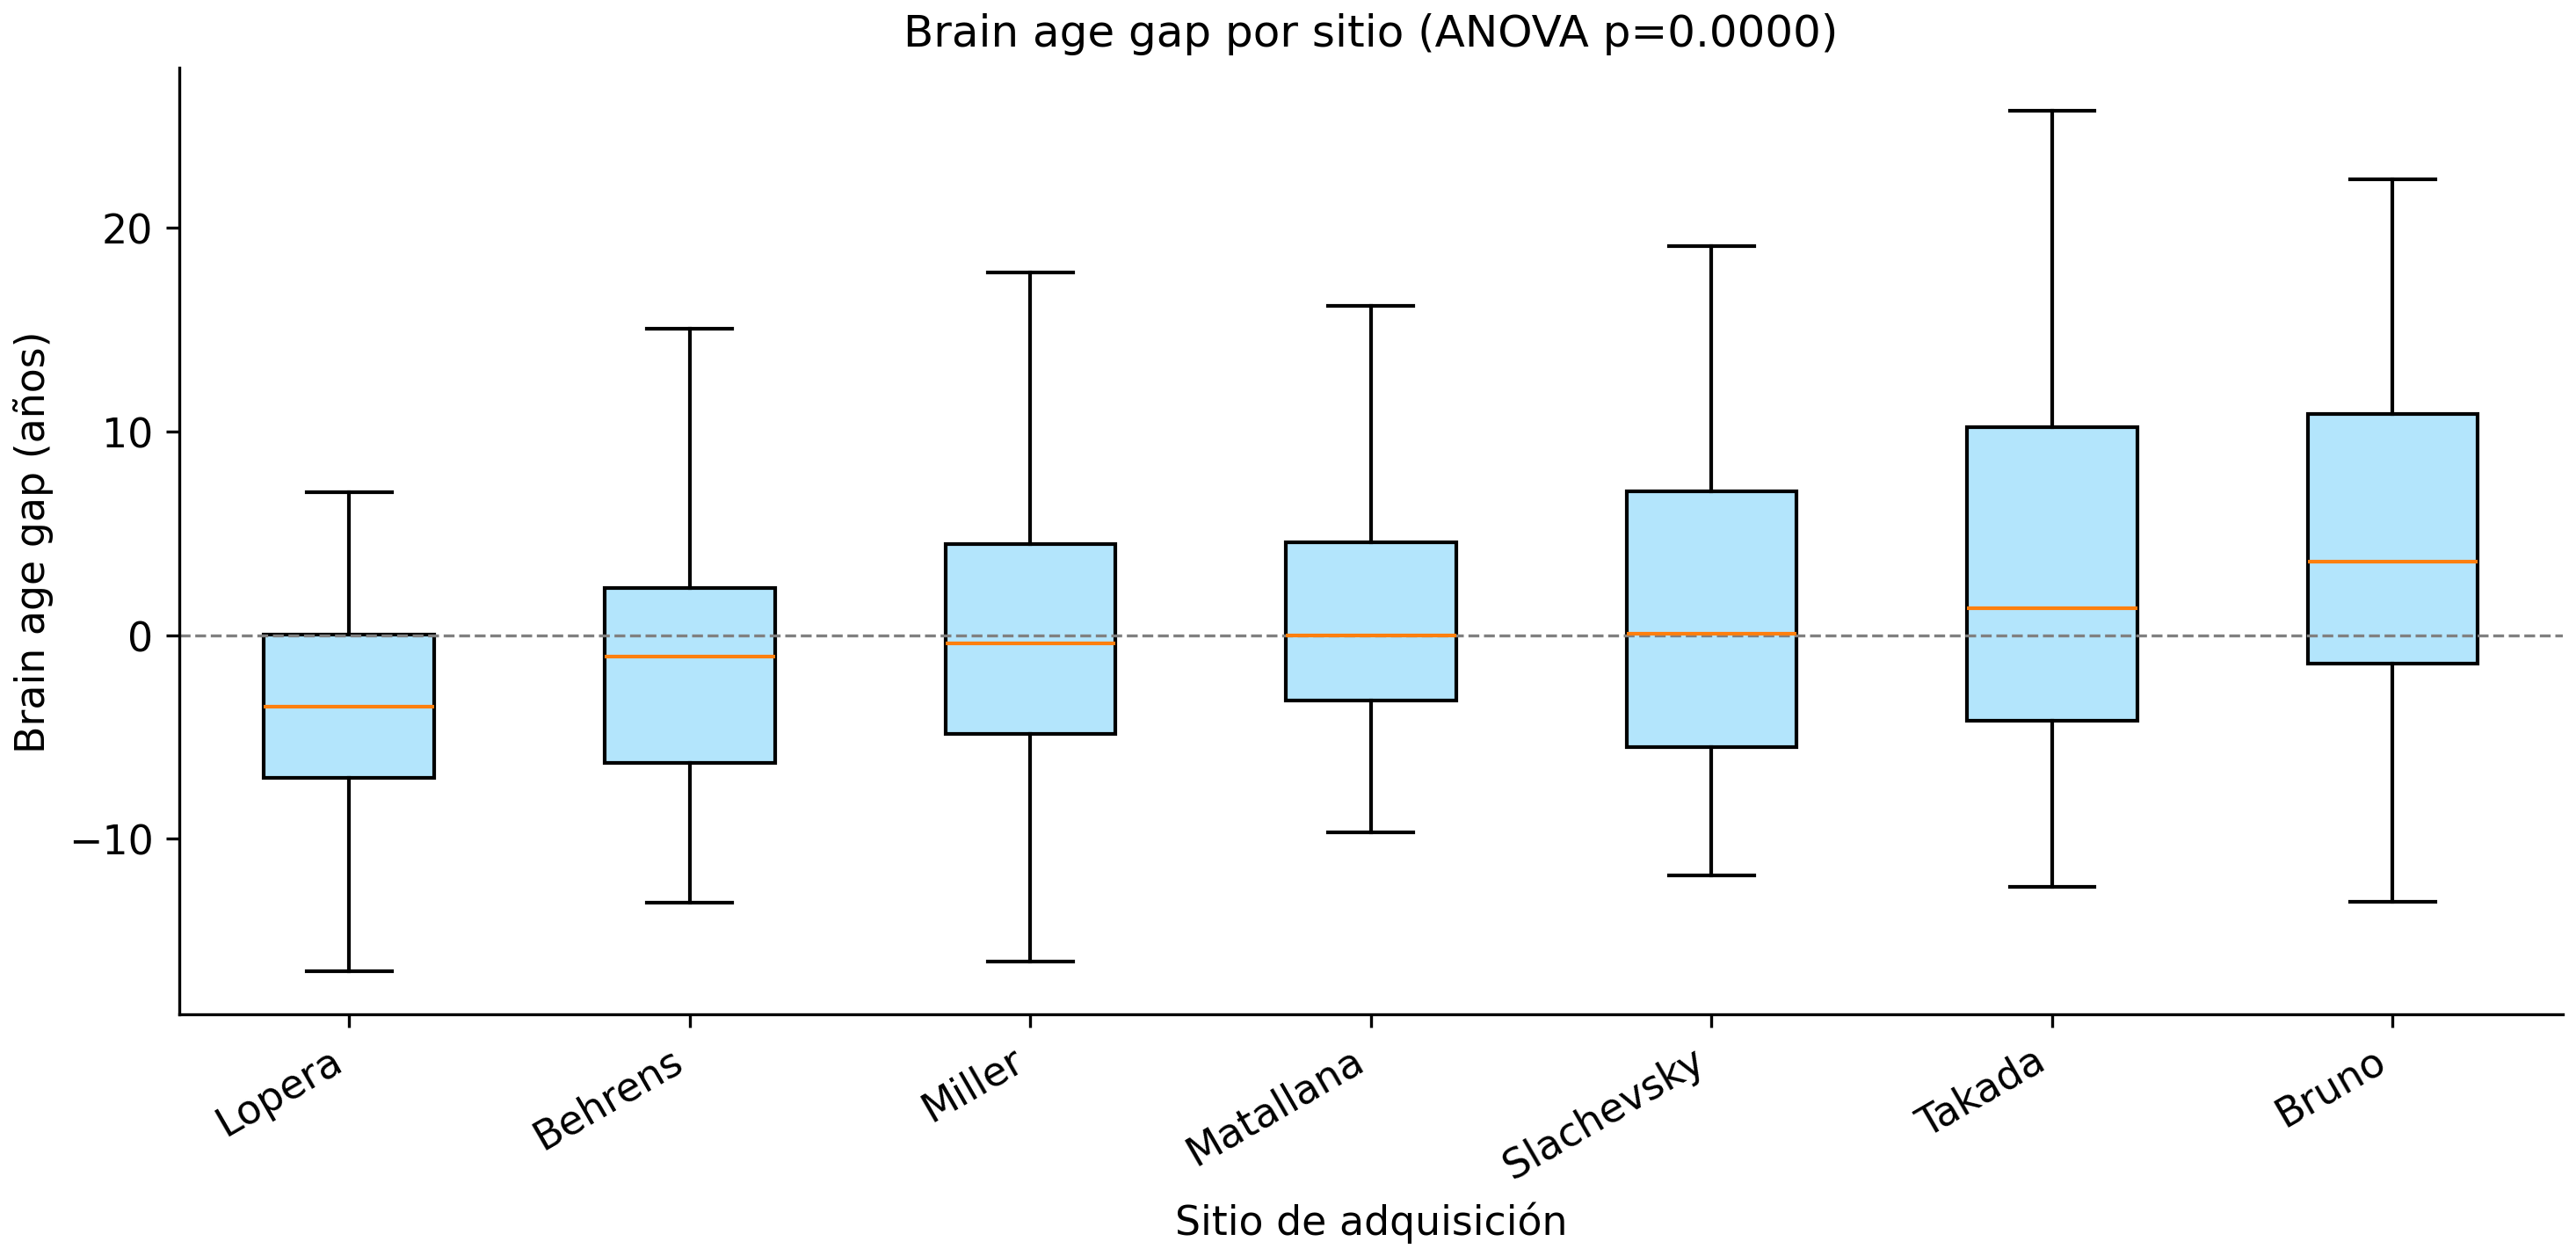
\includegraphics[width=0.85\textwidth]{06_resultados_discusion/images/demo_gap_by_site.png}
\caption{Distribución de la brain age gap por sitio de adquisición (sitios con $n \geq 20$). Las diferencias entre centros son estadísticamente significativas (ANOVA $p < 0{,}001$).}
\label{fig:demo_gap_by_site}
\end{figure}

La variabilidad entre sitios es considerable: la diferencia entre el sitio con mayor gap media (Bruno, $+4{,}30$ años) y el de menor (Lopera, $-3{,}64$ años) es de casi 8 años. Esta variabilidad inter-sitio refleja diferencias en los protocolos de adquisición, las características del escáner, la composición diagnóstica y las particularidades demográficas de cada centro. El análisis por marca de escáner reveló un patrón consistente: los sujetos adquiridos con escáneres Philips presentaron la gap media más alta ($+4{,}33$ años, $n = 47$ sujetos), seguidos por GE (gap media $+0{,}95$ años, $n = 289$) y Siemens (gap media $-0{,}26$ años, $n = 581$). Dado que Siemens concentra el 63\% de la muestra, el modelo aprendió predominantemente a partir de imágenes de esta marca; al recibir imágenes de Philips o GE, las diferencias técnicas entre escáneres pueden generar predicciones sistemáticamente sesgadas. Estos resultados subrayan la importancia de considerar técnicas de armonización entre sitios (como ComBat \cite{fortin2017harmonization}) en futuros trabajos con cohortes multicéntricas.

\subsection{Variables demográficas como features de predicción}
\label{sec:res_demo_ablacion}

Se evaluó si la inclusión de los años de educación y/o el sitio de adquisición como features adicionales mejora la predicción de edad. Para cada configuración, los hiperparámetros de XGBoost se optimizaron de forma independiente con Optuna (100 trials, 5-fold CV), garantizando que cada modelo disponga de parámetros ajustados a su espacio de features específico. Dado que estas variables no están disponibles para todos los sujetos, las configuraciones que las utilizan operan sobre una cohorte reducida. La Tabla~\ref{tab:demo_ablation} presenta los resultados.

\begin{table}[H]
\centering
\caption{Ablaciones con variables demográficas como features adicionales, cada una con hiperparámetros de XGBoost optimizados independientemente con Optuna. La reducción de $N$ se debe a la disponibilidad parcial de educación y sitio ($\sim$75\% de la cohorte). Se resalta en negrita la configuración con mejor MAE.}
\label{tab:demo_ablation}
\resizebox{\textwidth}{!}{%
\begin{tabular}{lrrrrrr}
\toprule
\textbf{Configuración} & \textbf{$n_{\text{train}}$} & \textbf{$n_{\text{test}}$} & \textbf{Features} & \textbf{MAE} & \textbf{$R^2$} & \textbf{Pearson} \\
\midrule
VAE + T1w                    & 1120 & 125 & 180 & 5,62 & 0,411 & 0,644 \\
VAE + T1w + educación        &  842 &  91 & 181 & 5,33 & 0,502 & 0,711 \\
VAE + T1w + sitio            &  848 &  93 & 189 & 5,37 & 0,538 & 0,744 \\
\textbf{VAE + T1w + edu + sitio} & \textbf{842} & \textbf{91} & \textbf{190} & \textbf{5,17} & \textbf{0,523} & \textbf{0,725} \\
\bottomrule
\end{tabular}}
\end{table}

La configuración que combina educación y sitio con hiperparámetros optimizados independientemente alcanza un MAE de 5,17 años, una mejora de 0,45 años respecto al baseline (5,62). Todas las configuraciones con variables demográficas superan al baseline en todas las métricas. La configuración con sitio obtiene el mejor $R^2$ (0,538), mientras que la combinación de educación y sitio logra el mejor MAE. Estos resultados deben interpretarse con cautela, ya que las configuraciones con demográficos operan sobre una cohorte reducida ($n_{\text{test}} = 91$--$93$ vs.~$125$) compuesta por los sujetos que disponen de los datos correspondientes; la diferencia en la composición del conjunto de test puede contribuir a parte de las diferencias observadas.

\subsubsection{Importancia de las variables demográficas en la predicción}

La Figura~\ref{fig:demo_importance} muestra las 20 features más importantes según XGBoost para las tres configuraciones con variables demográficas. En la configuración con educación únicamente, la variable \texttt{education} aparece entre las features más relevantes, lo que indica que el modelo aprovecha activamente esta información para refinar sus predicciones. En las configuraciones que incluyen sitio, las variables de sitio codificadas mediante one-hot (véase Sección~\ref{sec:demo_method}) también aparecen entre las features más importantes; en particular, \texttt{site\_Miller} ocupa consistentemente las primeras posiciones. La prominencia de \texttt{site\_Miller} se explica por su tamaño: con 400 sujetos, representa aproximadamente el 42\% de la subcohorte con información de sitio. El modelo aprende a reconocer las características propias de las imágenes de este centro (asociadas a su escáner, protocolo y población) y utiliza la variable binaria de sitio como un indicador que distingue ``imagen típica de Miller'' del resto, capturando así diferencias técnicas y demográficas sistemáticas. Que una sola variable categórica supere en importancia a muchas features de neuroimagen evidencia la magnitud de la variabilidad multicéntrica en la cohorte. En la configuración combinada (educación + sitio), ambas fuentes de información contribuyen de forma complementaria: las features de neuroimagen (T1w y embeddings del VAE) siguen dominando, pero las variables demográficas aportan señal adicional que reduce el error de predicción.

\begin{figure}[H]
\centering
\begin{subfigure}[b]{0.48\textwidth}
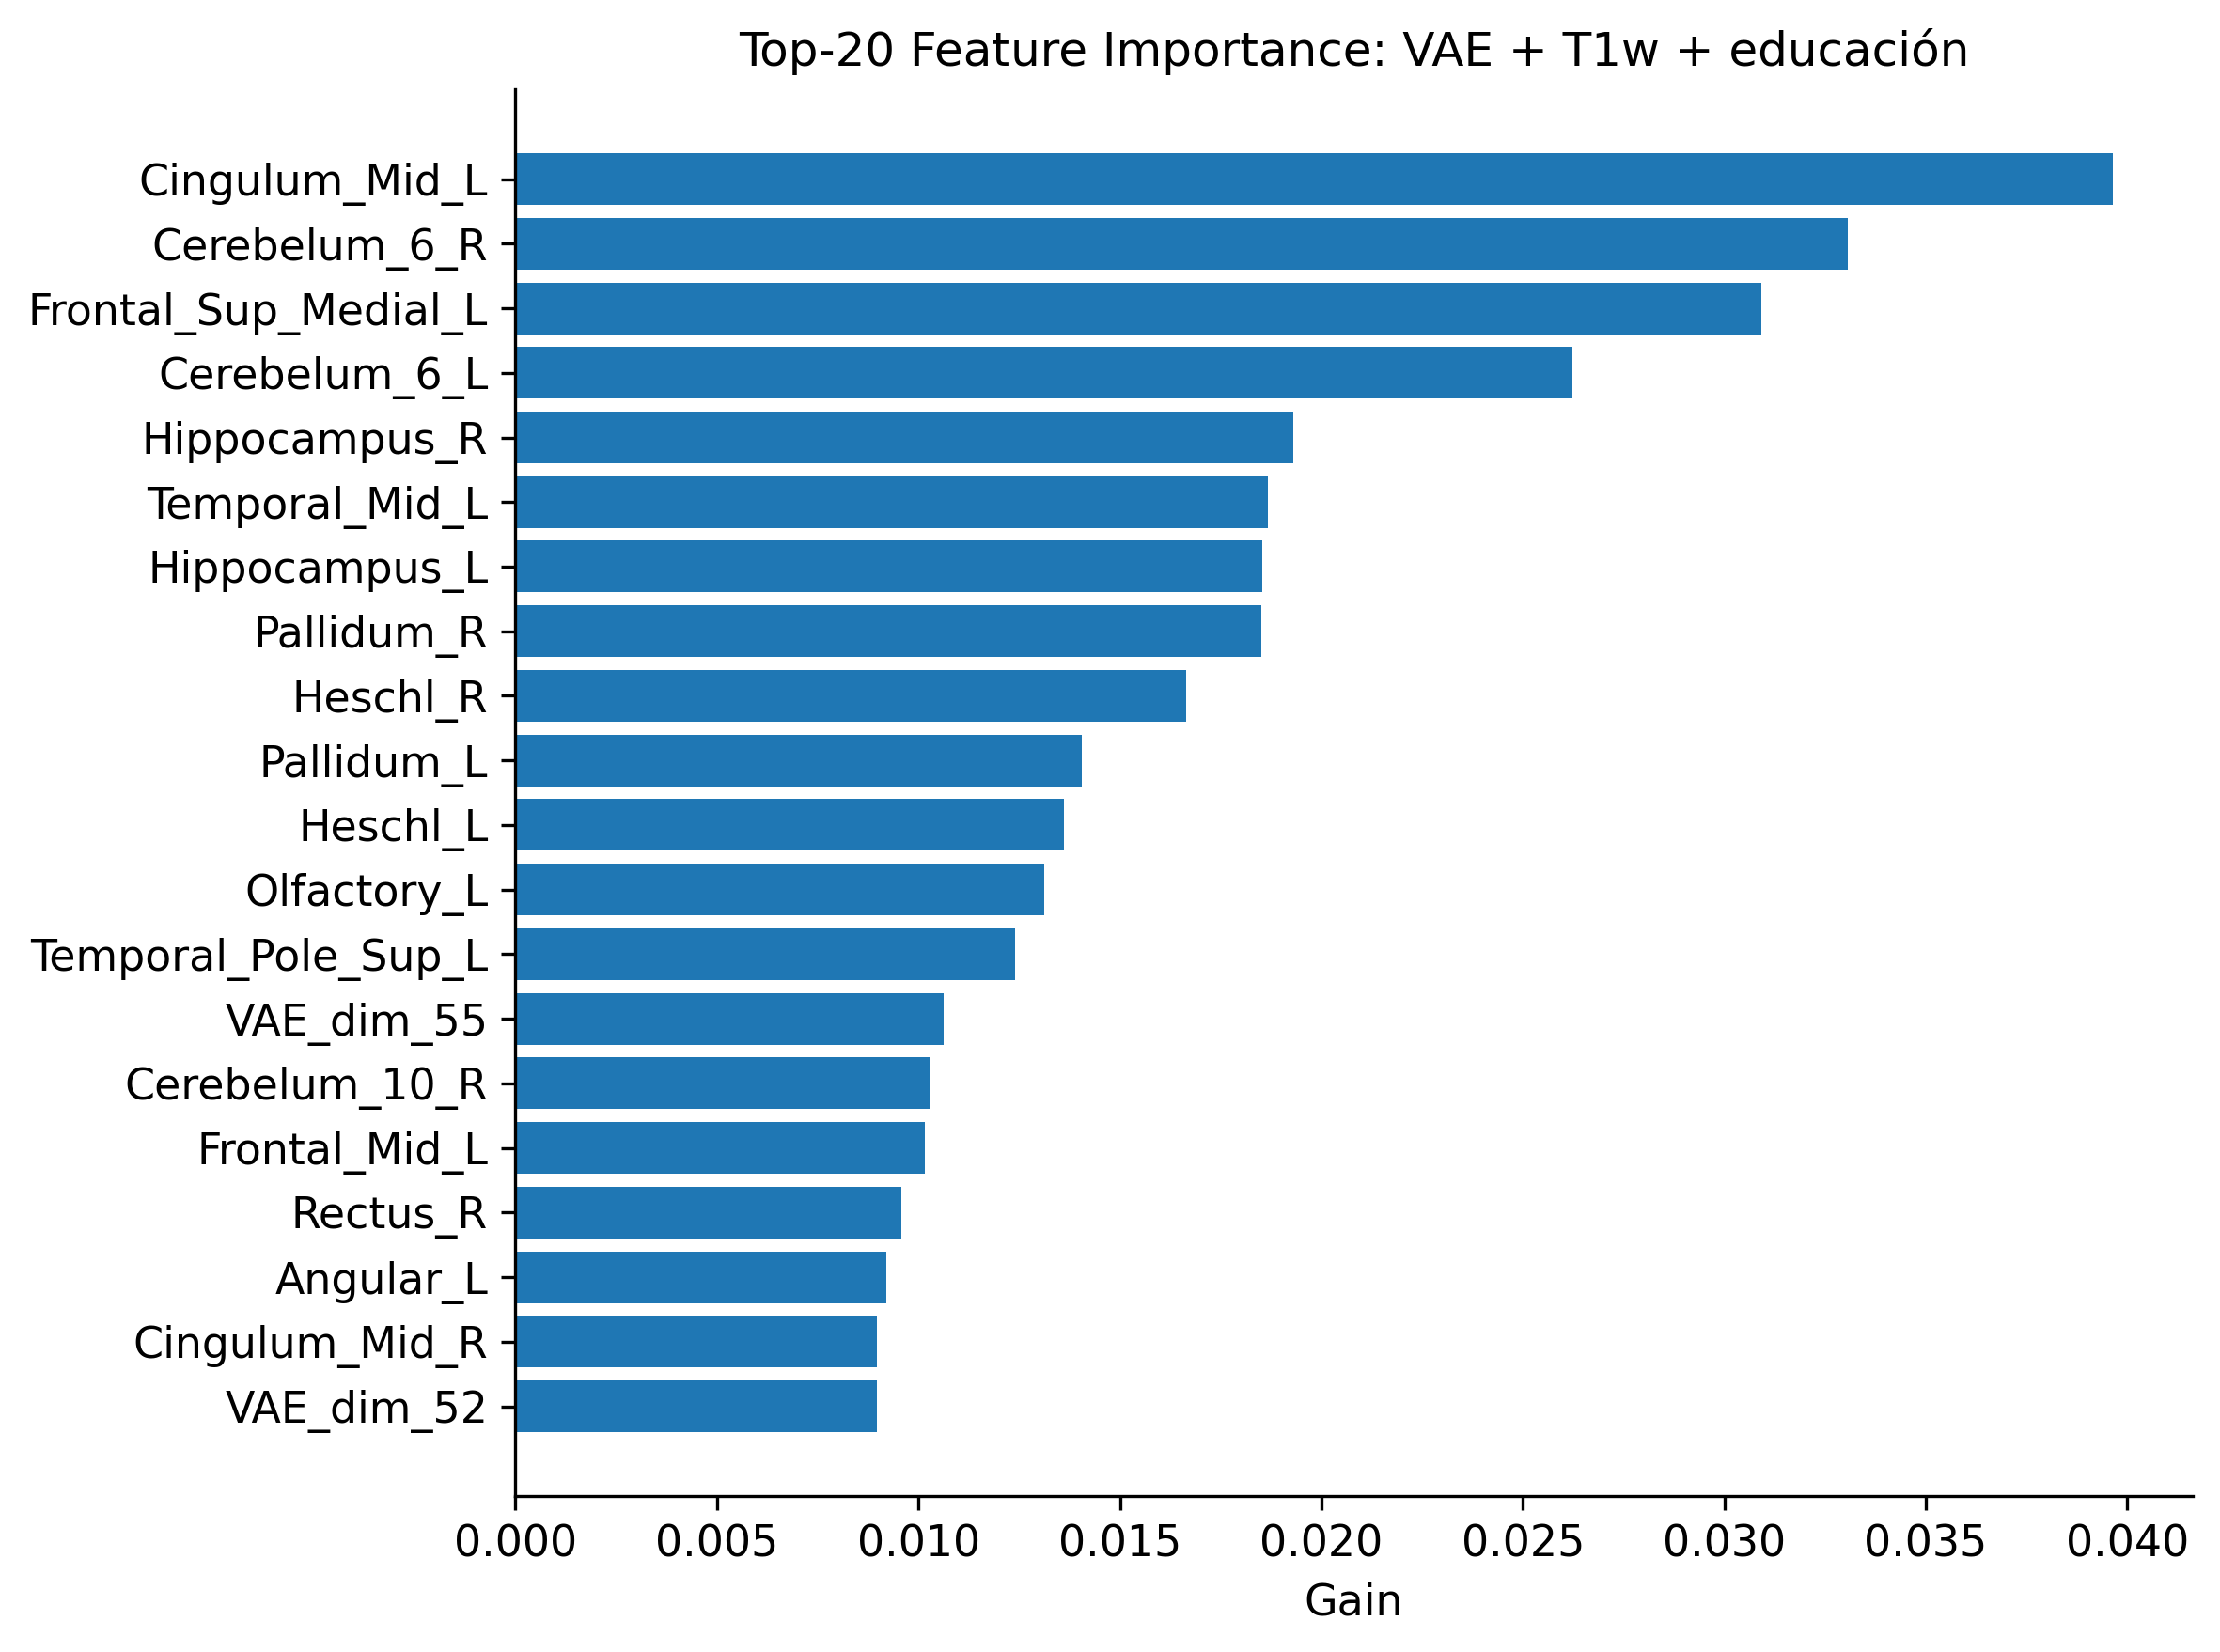
\includegraphics[width=\textwidth]{06_resultados_discusion/images/demo_importance_VAE__T1w__educacion.png}
\caption{VAE + T1w + educación}
\end{subfigure}
\hfill
\begin{subfigure}[b]{0.48\textwidth}
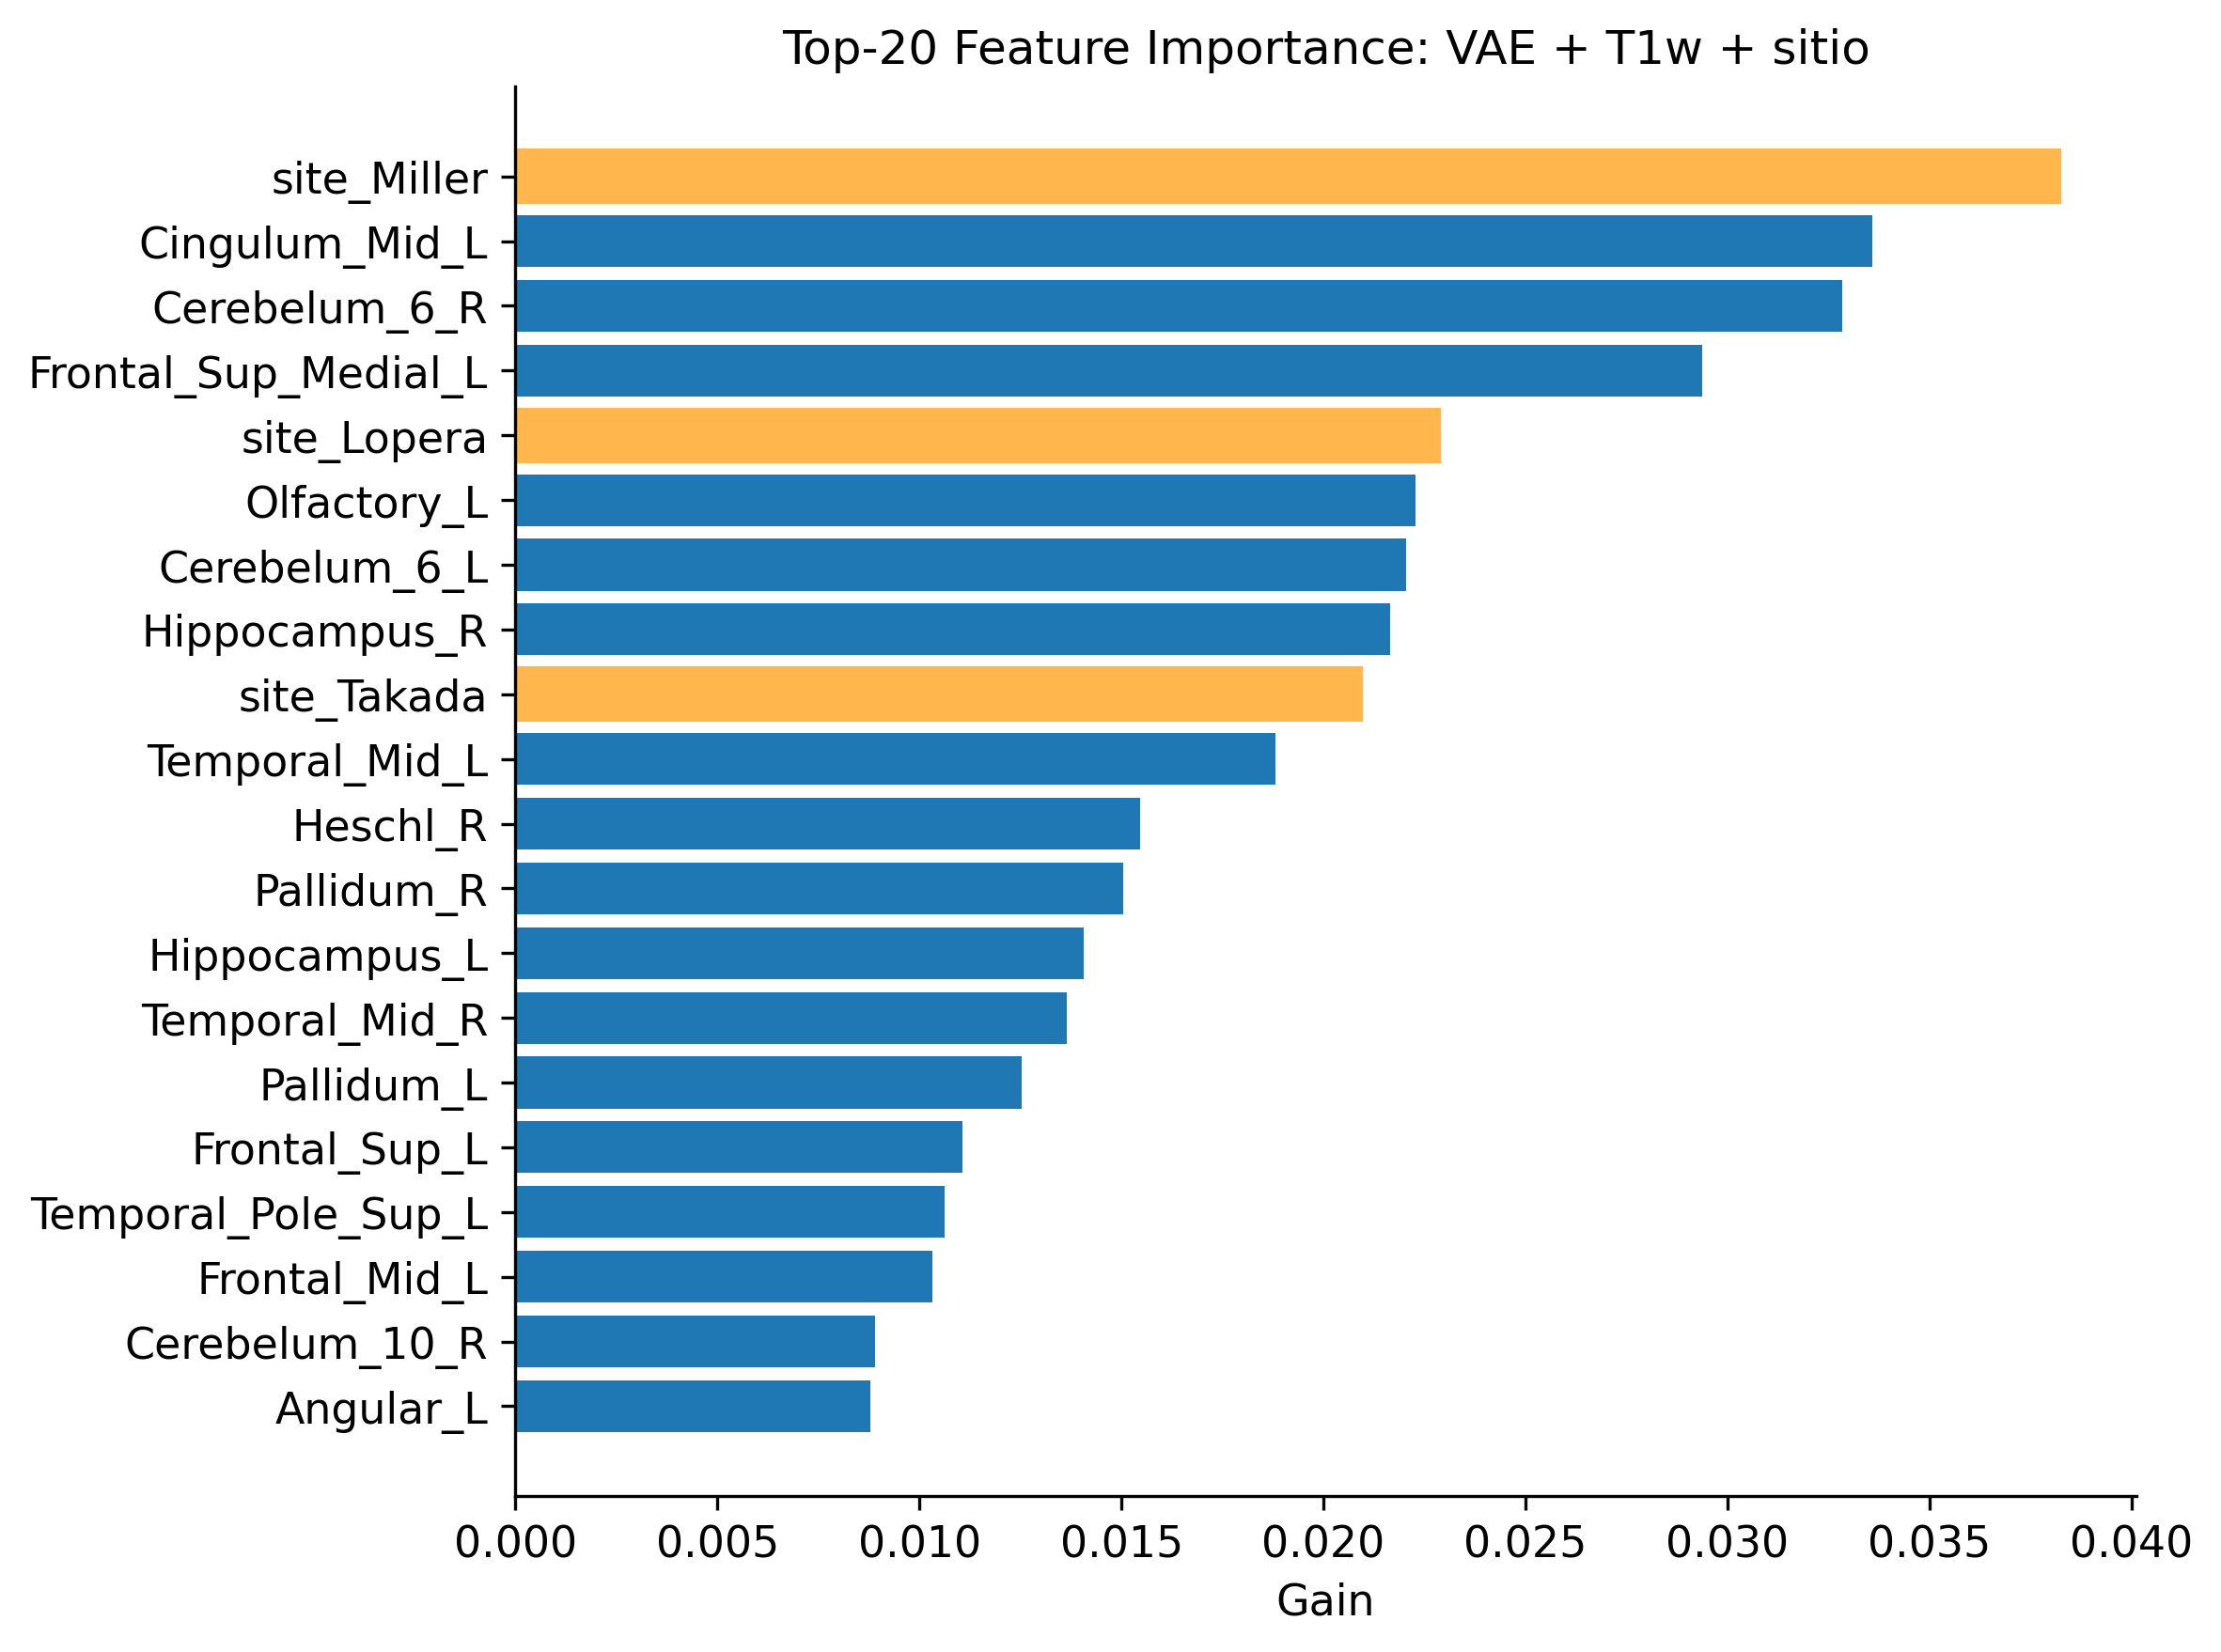
\includegraphics[width=\textwidth]{06_resultados_discusion/images/demo_importance_VAE__T1w__sitio.png}
\caption{VAE + T1w + sitio}
\end{subfigure}

\vspace{0.5cm}
\begin{subfigure}[b]{0.48\textwidth}
\centering
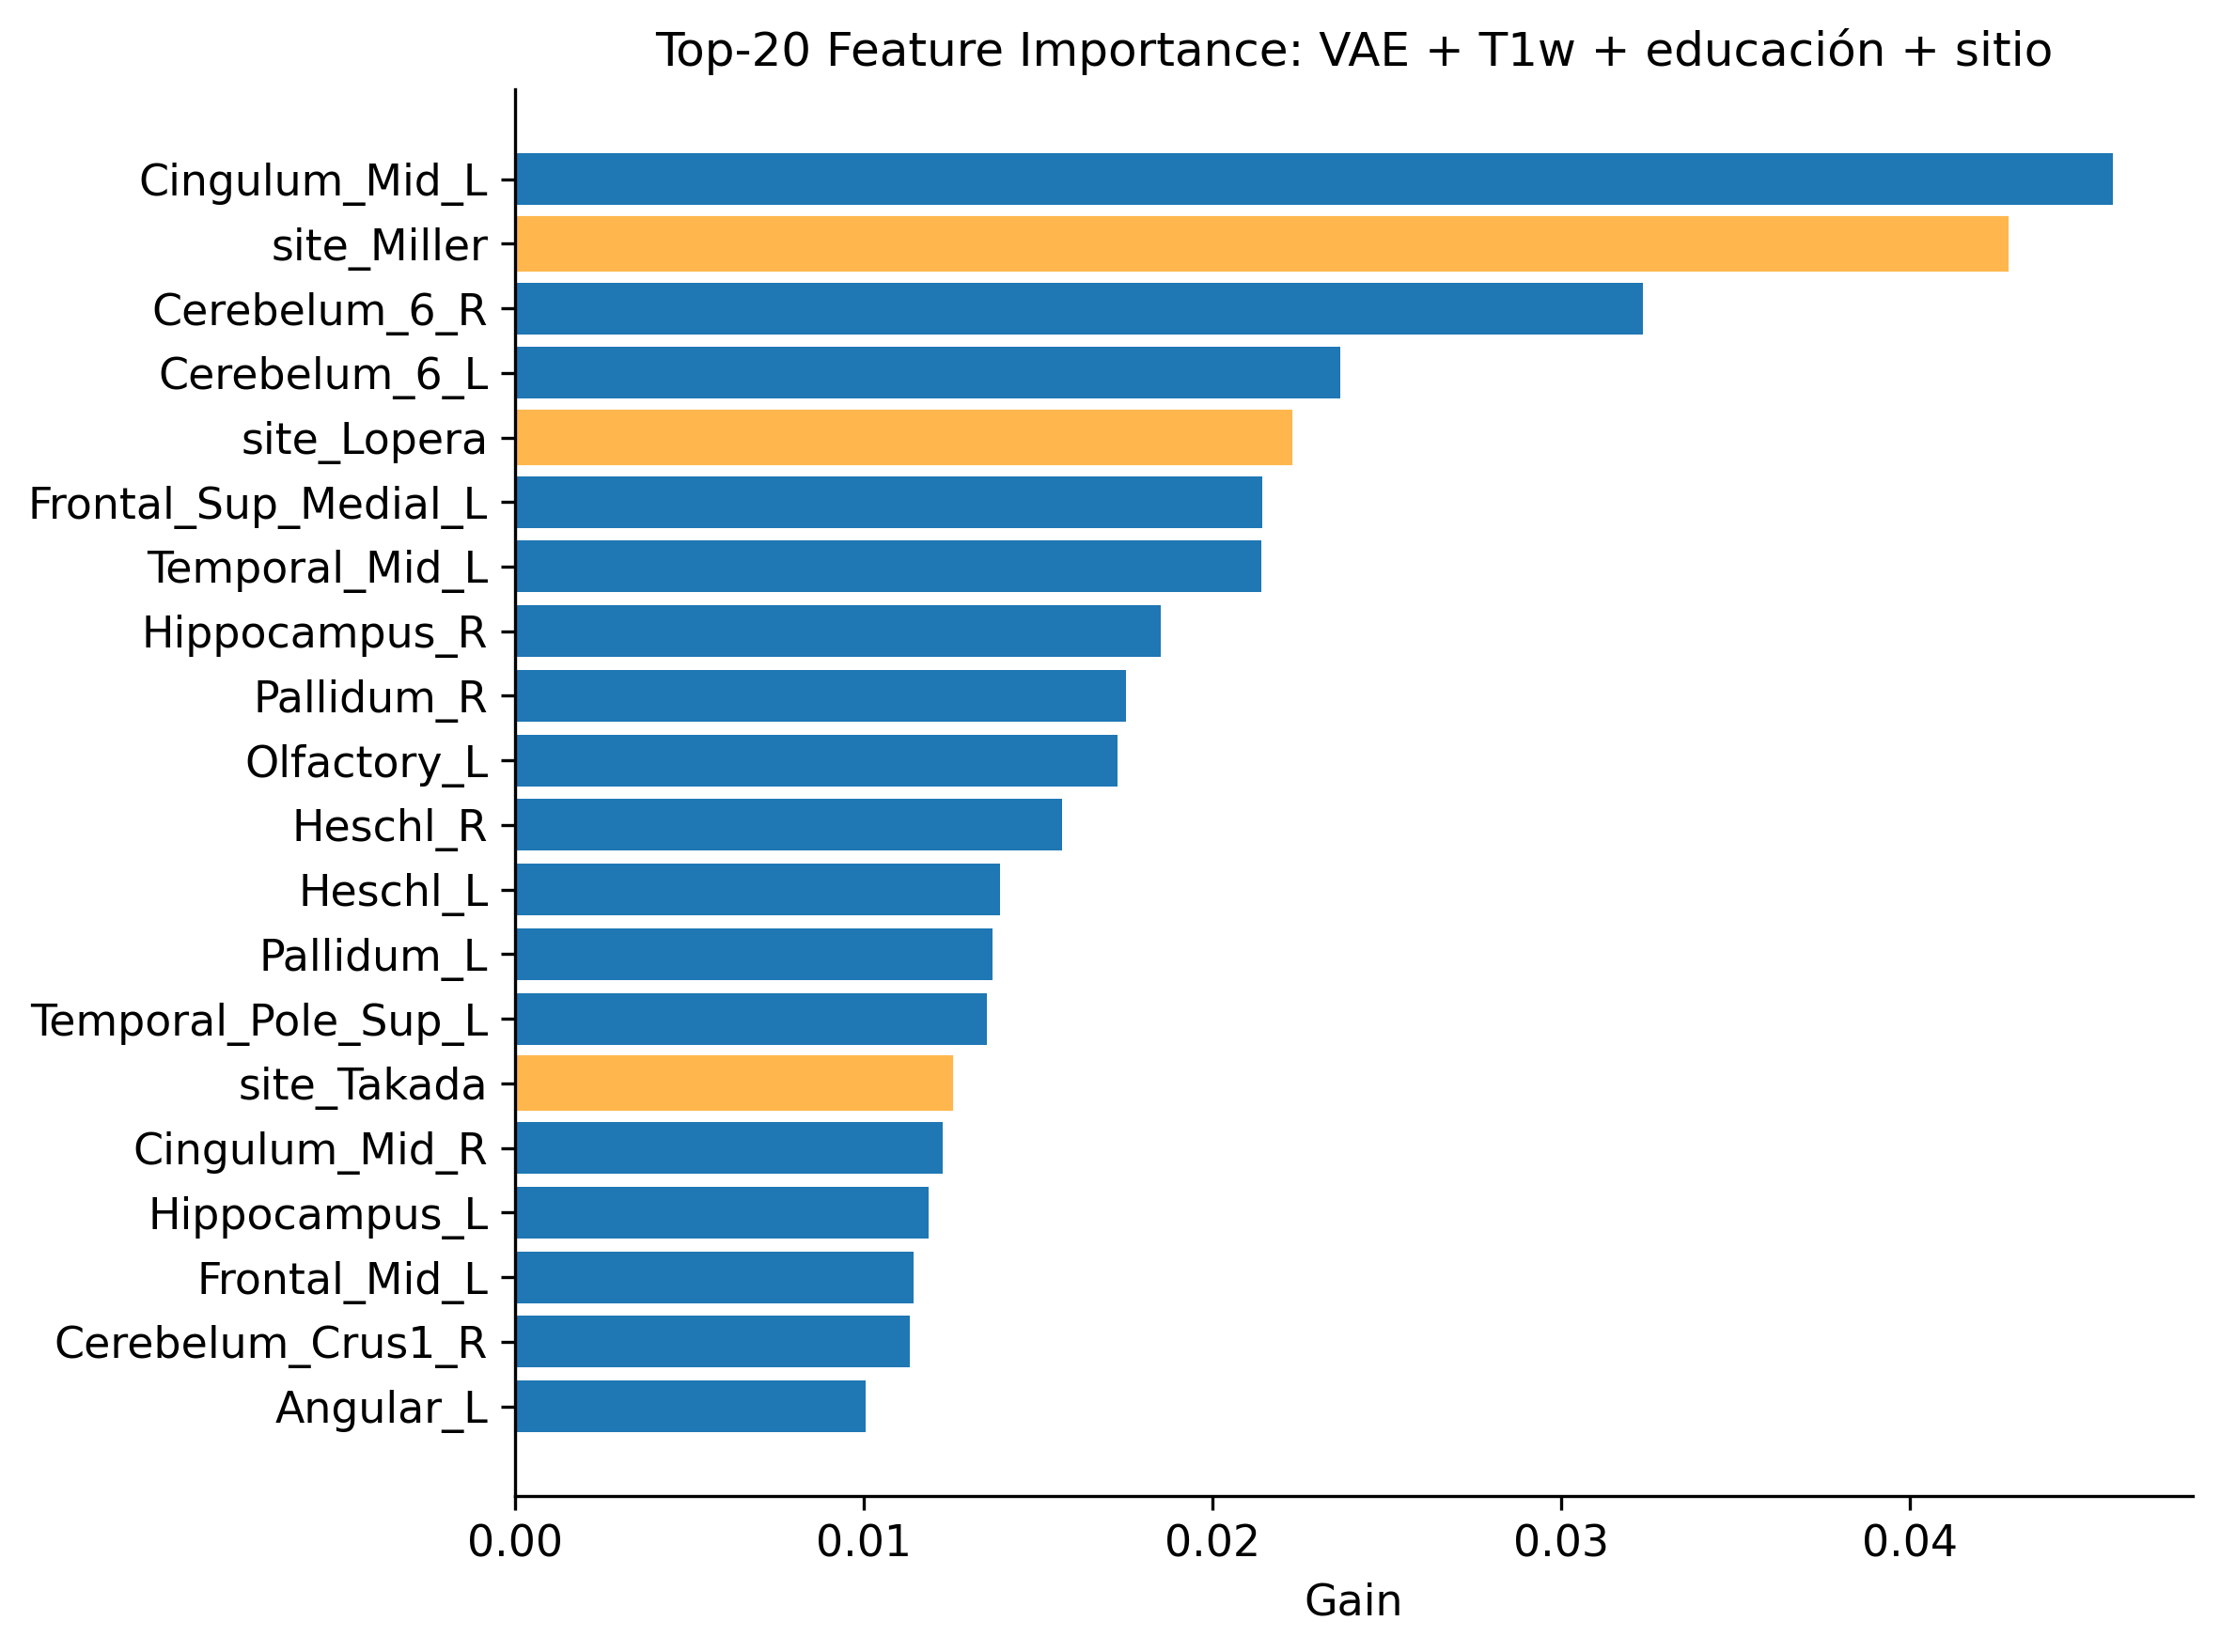
\includegraphics[width=\textwidth]{06_resultados_discusion/images/demo_importance_VAE__T1w__educacion__sitio.png}
\caption{VAE + T1w + educación + sitio}
\end{subfigure}
\caption{Top 20 features por importancia (XGBoost \textit{gain}) para cada configuración con variables demográficas. Las features con nombre anatómico (p.~ej.\ Cerebellum\_6\_R) corresponden a volúmenes T1w del atlas AAL-116. Las etiquetadas como VAE\_dim\_$N$ son dimensiones del espacio latente del $\beta$-VAE, que codifican patrones de conectividad funcional aprendidos de forma no supervisada; al no representar una región cerebral individual sino una combinación de conexiones, no admiten una interpretación anatómica directa. Las features demográficas (\texttt{education}, \texttt{site\_X}) aparecen entre las más relevantes junto con las de neuroimagen.}
\label{fig:demo_importance}
\end{figure}

Una regresión lineal de la brain age gap sobre las variables demográficas reveló que la educación por sí sola explica menos del 1\% de la varianza de la gap ($R^2 = 0{,}005$). Al agregar sexo y diagnóstico, la varianza explicada sube al 2,6\%, y al incluir el sitio alcanza el 8,0\%. La varianza explicada ($R^2$) indica qué porcentaje de la variabilidad total de la variable respuesta es capturado por el modelo: un $R^2 = 0{,}08$ (8\%) significa que las variables demográficas dan cuenta de solo el 8\% de las diferencias observadas en la brain age gap, mientras que el 92\% restante se debe a otros factores (diferencias neurobiológicas reales, ruido de medición, etc.). Esto confirma que el sitio de adquisición es el factor demográfico con mayor influencia sobre la gap, actuando como un confundidor que captura diferencias técnicas y poblacionales entre centros.


\section{Discusión}
\label{sec:discusion}

\subsection{Rendimiento en contexto e integración multimodal}

El modelo principal obtuvo un MAE de 5,62 años en el conjunto de test. Este resultado se encuentra dentro del rango típico reportado en la literatura de estimación de brain age, donde los estudios con datasets de tamaño comparable ($N \approx 1000\text{--}2000$) reportan valores de MAE entre 4 y 8 años \cite{franke2010estimating}. Los estudios basados en cohortes significativamente mayores ($N > 10\,000$), como UK Biobank, han alcanzado valores de MAE entre 2 y 4 años, beneficiándose de la mayor cantidad de datos y de la homogeneidad de los protocolos de adquisición. Es importante señalar que la mayoría de estos trabajos entrenan sus modelos exclusivamente sobre controles sanos, mientras que el presente pipeline fue entrenado sobre la cohorte completa (CN, AD y FTD). Entrenar con sujetos que presentan patologías neurodegenerativas introduce mayor heterogeneidad en los patrones de envejecimiento, lo que hace que el problema de regresión sea más difícil. Que el modelo alcance un MAE comparable al de estudios que solo entrenan con controles sanos sugiere que el pipeline logra capturar patrones generales de envejecimiento aun en presencia de esta variabilidad adicional. Por otro lado, la cohorte RedLaT integra datos de múltiples centros latinoamericanos con protocolos potencialmente heterogéneos, lo que introduce una fuente de ruido adicional y hace que la comparación directa con otros estudios deba interpretarse con cautela.

La combinación de conectividad funcional (vía $\beta$-VAE) con datos estructurales T1w mejora la predicción respecto al uso de cualquiera de las dos fuentes por separado: la mejora de 0,27 años en MAE y de 0,045 en $R^2$ al agregar los embeddings del VAE a T1w es consistente y se observa en todas las métricas. Al mismo tiempo, los embeddings por sí solos resultan insuficientes (MAE = 7,01), lo que sugiere que la conectividad funcional es una fuente de información más ruidosa que los datos estructurales y se beneficia de la complementación. La fusión a nivel de features permite que el regresor identifique las combinaciones más informativas de ambas fuentes.

La comparación entre regresores (Sección~\ref{sec:res_regresores}) refuerza esta observación: Ridge, SVR y XGBoost alcanzan prácticamente el mismo rendimiento (diferencia máxima de 0,13 años en MAE), lo que sugiere que, una vez construidas representaciones de calidad, la elección del regresor tiene un impacto marginal. Este resultado es coherente con la observación de que las features del VAE son suaves y continuas, un escenario favorable para distintas familias de modelos.

\subsection{Modelado no lineal y estrategias de entrenamiento}

Un resultado notable es la equivalencia práctica entre PCA y $\beta$-VAE como métodos de reducción de dimensionalidad (Sección~\ref{sec:res_pca}): ambos alcanzan un MAE $\approx$ 5,6 y un $R^2 \approx$ 0,42, con diferencias menores a 0,02 en todas las métricas. Esto sugiere que la información relevante para la predicción de edad en las matrices FC es capturada en buena medida por las direcciones de máxima varianza (componentes principales), y que un regresor potente como XGBoost puede extraer patrones no lineales incluso a partir de proyecciones lineales. Sin embargo, la reducción de dimensionalidad sí es necesaria: la comparación con features crudos de FC (Sección~\ref{sec:res_raw_fc}) muestra que, aun con hiperparámetros optimizados específicamente para la entrada de alta dimensionalidad, el pipeline sin compresión obtiene un MAE de 6,00 frente a 5,62 del pipeline comprimido, y un $R^2$ de 0,354 frente a 0,411. Es decir, el paso clave es la reducción de 6670 a 64 dimensiones, no el carácter lineal o no lineal de dicha reducción.

Es importante contextualizar la equivalencia PCA--VAE. La elección del $\beta$-VAE como componente del pipeline siguió la tendencia predominante en la literatura de neuroimagen, donde los autoencoders variacionales se han adoptado ampliamente para modelar datos cerebrales de alta dimensionalidad. La comparación con PCA fue realizada a posteriori como una validación de la necesidad de la complejidad no lineal del VAE. Además, la exploración del espacio de hiperparámetros del VAE fue necesariamente limitada: 70 trials de Optuna sobre un espacio combinatorio que incluye la dimensión latente, el número y tamaño de capas ocultas, $\beta$, dropout, learning rate, épocas de warmup y tipo de embedding. Con una exploración más exhaustiva o con técnicas de búsqueda más sofisticadas, el VAE podría potencialmente superar a PCA, especialmente a medida que el tamaño de la muestra aumente y las representaciones no lineales dispongan de más datos para capturar patrones sutiles. En cualquier caso, el resultado actual es informativo y consistente con los hallazgos de Monti et al.\ y More et al.\ discutidos en la Sección~\ref{sec:res_pca}. El presente trabajo extiende esas observaciones al mostrar que, para esta cohorte y esta dimensionalidad, la complejidad del VAE no aporta una ventaja mensurable en la predicción de edad, aunque sí ofrece capacidades adicionales (generación, reconstrucción) que un método puramente lineal no puede proporcionar.

En cuanto a la estrategia de entrenamiento, el modelo entrenado exclusivamente en controles sanos (Sección~\ref{sec:res_cn_only}) fue evaluado sobre la totalidad de los pacientes AD ($n = 422$) y FTD ($n = 297$), ya que ninguno de ellos fue utilizado durante el entrenamiento. A pesar de este mayor poder estadístico, los $R^2$ fueron negativos en ambos grupos clínicos, la brain age gap mostró una dirección inconsistente entre AD ($-1{,}86$~años) y FTD ($+1{,}84$~años), y las correlaciones de Pearson fueron inferiores a 0,2. Esto indica que, con $N = 473$ sujetos CN, el modelo no logra aprender la relación entre neuroimagen y edad con la precisión suficiente para que las desviaciones de esa norma constituyan un biomarcador confiable. Este resultado no invalida la estrategia CN-only en general, pero sugiere que requiere cohortes considerablemente mayores \cite{smith2019estimation}.

Resulta alentador, no obstante, que el modelo CN-only entrenado con variables demográficas (Sección~\ref{sec:res_cn_demo}) ---aun con solo 337 sujetos CN--- produce gaps consistentemente positivas en ambos grupos clínicos (AD: $+0{,}70$; FTD: $+4{,}11$), la dirección esperada en neurodegeneración. Aunque el tamaño de muestra es insuficiente para extraer conclusiones definitivas, este resultado sugiere que la inclusión de información demográfica podría facilitar la construcción de un biomarcador de envejecimiento cerebral cuando se disponga de cohortes CN más amplias.

\subsection{Variables demográficas y variabilidad multicéntrica}

El análisis del impacto de variables demográficas (Sección~\ref{sec:res_demograficas}) reveló que el sitio de adquisición es el factor con mayor influencia sobre la brain age gap, explicando el 8\% de su varianza cuando se combina con educación, sexo y diagnóstico. Las diferencias entre sitios alcanzan casi 8 años de gap media, lo que pone de manifiesto la necesidad de técnicas de armonización en cohortes multicéntricas. En la cohorte RedLaT, esta variabilidad inter-sitio refleja no solo diferencias técnicas (escáneres, protocolos) sino también diferencias poblacionales propias de cada centro latinoamericano.

Al incorporar la educación y el sitio como features adicionales del modelo con hiperparámetros optimizados independientemente mediante Optuna (Sección~\ref{sec:res_demo_ablacion}), se obtuvo un MAE de 5,17 años, la mejor configuración evaluada en este trabajo. Este resultado indica que las variables demográficas contienen información predictiva sobre la edad que no está completamente capturada por las features de neuroimagen. El análisis de importancia de features confirmó que tanto la educación como las variables de sitio se posicionan entre las features más relevantes del modelo, aportando señal complementaria a los embeddings del VAE y los volumenes T1w.

La educación, utilizada como indicador del nivel socioeconómico, mostró una correlación significativa con la gap únicamente en pacientes con AD ($r = +0{,}165$, $p = 0{,}002$). La dirección positiva (más educación $\rightarrow$ gap más alta) podría explicarse por un efecto de reserva cognitiva: los pacientes con mayor educación mantienen el funcionamiento cognitivo durante más tiempo, accediendo al diagnóstico en estadios más avanzados de la neurodegeneración, cuando la atrofia cerebral es más pronunciada. En controles sanos, la tendencia negativa ($r = -0{,}067$, no significativa) es consistente con la hipótesis de que la educación ejerce un efecto neuroprotector, aunque la señal es demasiado débil para alcanzar significancia con esta muestra. Estos resultados son relevantes en el contexto latinoamericano, donde la variabilidad en los niveles educativos es considerable y puede modular tanto el acceso al diagnóstico como la expresión clínica de la neurodegeneración.

\subsection{Limitaciones}
\label{sec:limitaciones}

El trabajo presenta varias limitaciones que conviene considerar. La más relevante es el tamaño de la cohorte: con $N = 1245$ sujetos, el dataset es significativamente menor que los empleados en estudios de referencia, lo que limita tanto la capacidad de generalización como el rendimiento del modelo (reflejado en un $R^2$ moderado de 0,411). Relacionado con esto, el modelo entrenado solo en CN mostró señales inconsistentes al evaluar la brain age gap en las poblaciones clínicas, lo que impidió su uso como biomarcador confiable. Los resultados exploratorios con variables demográficas en el modelo CN-only son prometedores (gaps positivas en AD y FTD), pero se basan en solo 337 sujetos de entrenamiento y requieren validación con cohortes más amplias.

El análisis de variables demográficas se limitó a las disponibles en la cohorte con cobertura suficiente (educación, sitio y marca de escáner). Otras variables de interés ---como el nivel de ingreso, la ocupación o el estatus socioeconómico--- no estaban disponibles o presentaban una cobertura insuficiente, lo que impidió un análisis más exhaustivo de los factores sociodemográficos que podrían modular el envejecimiento cerebral en poblaciones latinoamericanas.

Desde el punto de vista metodológico, se utilizó el atlas AAL con 116 regiones, que es una parcellación relativamente gruesa. Sería interesante evaluar el pipeline con atlas de mayor resolución, como el de Schaefer et al.\ \cite{schaefer2018local} (disponible con 100 a 1000 parcelas), que podrían capturar patrones más finos de conectividad funcional, aunque su impacto sobre la predicción de edad no está garantizado y requeriría una evaluación empírica. Además, no se aplicaron técnicas de armonización entre sitios (como ComBat \cite{fortin2017harmonization}) para reducir la variabilidad introducida por los diferentes protocolos de adquisición de los centros de RedLaT.

En relación con la optimización del VAE, la búsqueda de hiperparámetros mediante Optuna exploró 70 configuraciones de un espacio combinatorio extenso. Si bien el número de trials es razonable dado el costo computacional de entrenar cada VAE, representa una fracción pequeña del espacio total. Esta exploración limitada podría explicar en parte la equivalencia observada con PCA: no puede descartarse que una configuración del VAE no explorada hubiera producido representaciones superiores a las componentes principales.

Por último, el pipeline utiliza un enfoque en dos etapas donde el VAE y el XGBoost se optimizan de forma separada. Arquitecturas de deep learning end-to-end, como redes de grafos sobre matrices de conectividad o redes convolucionales 3D sobre volúmenes T1w, podrían integrar ambas etapas y potencialmente mejorar el rendimiento, aunque requieren muestras mayores para entrenarse de forma efectiva. \cleardoublepage

% Cap 7: Conclusiones y trabajo futuro
\chapter{Conclusiones y trabajo futuro}
\label{chapter:conclu}

\section{Conclusiones}

En este trabajo se desarrolló un pipeline de estimación de edad cerebral a partir de datos multimodales de neuroimagen, combinando conectividad funcional derivada de fMRI en reposo con medidas estructurales de materia gris obtenidas mediante imágenes T1w. El enfoque propuesto integra un $\beta$-VAE para la reducción de dimensionalidad no lineal de las matrices de conectividad funcional con un modelo XGBoost para la predicción supervisada de la edad, y fue evaluado sobre una cohorte de $N = 1245$ sujetos de la Red Latinoamericana de Investigación en Neurodegeneración (RedLaT).

El modelo principal alcanzó un MAE de 5,62 años y un $R^2$ de 0,411 sobre un conjunto de test independiente, valores que se encuentran dentro del rango reportado en la literatura para datasets de tamaño comparable. Cabe destacar que la mayoría de los estudios previos entrenan sus modelos exclusivamente sobre controles sanos, mientras que en este trabajo el pipeline fue entrenado sobre la cohorte completa, incluyendo pacientes con AD y FTD. A pesar de la mayor heterogeneidad que esto introduce, el modelo alcanza un rendimiento comparable, lo que sugiere que el pipeline es capaz de capturar patrones generales de envejecimiento cerebral aun en presencia de variabilidad patológica. Estos resultados confirman que es posible estimar la edad cerebral de forma razonable a partir de datos multimodales recolectados en un contexto multi-céntrico latinoamericano.

Uno de los hallazgos más relevantes del trabajo es que la integración de ambas modalidades mejora la predicción respecto al uso de cualquiera de ellas por separado. El estudio de ablaciones mostró que agregar los embeddings del VAE a los datos T1w reduce el MAE en 0,27 años, lo que indica que la conectividad funcional captura patrones de envejecimiento que los volúmenes de materia gris no contienen. Al mismo tiempo, los embeddings del VAE por sí solos resultan insuficientes como única fuente de información, lo que refuerza la importancia de la estrategia multimodal.

La comparación entre PCA y el $\beta$-VAE reveló un resultado notable: ambos métodos alcanzan un rendimiento prácticamente idéntico cuando se combinan con XGBoost optimizado, con diferencias menores a 0,02 en todas las métricas. Esto indica que, con un regresor suficientemente potente, las componentes principales capturan tanta información relevante para la predicción de edad como las representaciones no lineales del VAE. La elección del $\beta$-VAE siguió la tendencia predominante en la literatura de neuroimagen computacional, y la exploración de su espacio de hiperparámetros fue necesariamente limitada; no puede descartarse que configuraciones no evaluadas logren un rendimiento superior, particularmente con cohortes de mayor tamaño. Sin embargo, la reducción de dimensionalidad sí es necesaria: la comparación con los features crudos de FC demostró que el pipeline sin compresión obtiene un MAE de 6,00 frente a 5,62. Es decir, el paso clave es comprimir las 6670 dimensiones a 64, independientemente de si la compresión es lineal o no lineal.

Otro aspecto relevante del diseño fue la decisión de optimizar los hiperparámetros del VAE utilizando la predicción de edad como objetivo downstream, en lugar de minimizar exclusivamente el error de reconstrucción. Se espera que esta estrategia favorezca representaciones latentes orientadas a capturar información relevante al envejecimiento, en lugar de priorizar una reconstrucción fiel de las matrices FC que podría incluir variabilidad no relacionada con la edad. Verificar esta hipótesis mediante una comparación directa entre ambos criterios de optimización constituye una línea de trabajo futuro interesante.

El análisis del impacto de variables demográficas reveló que el sitio de adquisición es el factor con mayor influencia sobre la brain age gap, con diferencias de casi 8 años entre centros, lo que subraya la necesidad de técnicas de armonización en cohortes multicéntricas. Los años de educación mostraron una correlación significativa con la gap en pacientes con AD, posiblemente reflejando un efecto de reserva cognitiva por el cual los pacientes más educados acceden al diagnóstico en estadios más avanzados. En controles sanos, la tendencia fue negativa pero no significativa, consistente con un posible efecto neuroprotector de la educación. La inclusión de educación y sitio como features del modelo logró reducir el MAE a 5,17 años ---la mejor configuración evaluada en este trabajo---, lo que demuestra que estas variables contienen información predictiva complementaria a las features de neuroimagen. Estos resultados son particularmente relevantes en el contexto latinoamericano, donde la variabilidad en los niveles educativos y en las condiciones de adquisición es mayor que en cohortes más homogéneas. Cabe destacar que el pipeline es modular y reutilizable: su estructura facilita la incorporación de nuevas variables demográficas o la adaptación a distintas cohortes.

Finalmente, el experimento de entrenamiento exclusivo en controles sanos puso de manifiesto una limitación del tamaño de la muestra: con solo 473 sujetos CN, el modelo produjo señales de brain age gap débiles e inconsistentes entre los grupos clínicos, insuficientes para funcionar como biomarcador. Se realizó además una optimización Optuna dedicada para descartar que la limitación fuera atribuible a hiperparámetros subóptimos, confirmando que el problema es el tamaño muestral. No obstante, un resultado alentador surgió al incluir variables demográficas en el modelo CN-only: las gaps clínicas resultaron consistentemente positivas en ambos grupos (la dirección esperada en neurodegeneración), lo que sugiere que la combinación de variables demográficas con neuroimagen podría facilitar la construcción de un biomarcador cuando se disponga de cohortes CN más amplias. El pipeline diseñado es reutilizable para este fin: basta con filtrar los datos de entrenamiento a controles sanos y ejecutar el mismo flujo de optimización y evaluación.

\section{Trabajo futuro}

A partir de las limitaciones identificadas y los resultados obtenidos, se plantean varias líneas de trabajo que podrían extender y mejorar el enfoque propuesto.

La limitación más directa de este trabajo es el tamaño de la cohorte. Incrementar el número de sujetos, particularmente de controles sanos, permitiría no solo mejorar la generalización del modelo sino también habilitar el cálculo confiable de la brain age gap como biomarcador clínico. Los resultados del modelo CN-only con variables demográficas ---donde gaps consistentemente positivas en AD y FTD emergieron con solo 337 sujetos CN--- sugieren que, con cohortes de $N > 2000$ CN, la combinación de neuroimagen con datos demográficos podría producir un biomarcador robusto. En la misma dirección, la aplicación de técnicas de armonización entre sitios (como ComBat \cite{fortin2017harmonization}) resulta especialmente relevante: el análisis de variables demográficas demostró que el sitio de adquisición es el mayor confundidor de la gap, con diferencias de hasta 8 años entre centros. La armonización reduciría esta variabilidad espuria y podría mejorar tanto la precisión del modelo como la interpretabilidad de la brain age gap como indicador clínico. Además, la extensión del análisis demográfico a variables no disponibles o no incorporadas en este trabajo ---como nivel de ingresos, ocupación, estatus socioeconómico y edad de inicio de la enfermedad (ao)--- permitiría una caracterización más completa de los factores que modulan el envejecimiento cerebral en poblaciones latinoamericanas; en cohortes futuras, la recolección sistemática de estas variables facilitaría su inclusión tanto en el modelo predictivo como en el análisis de la brain age gap.

Desde el punto de vista del preprocesamiento, sería interesante evaluar el pipeline con atlas de mayor resolución que el AAL de 116 regiones. Parcelaciones de mayor resolución, como la de Schaefer et al.\ \cite{schaefer2018local} (disponible con hasta 1000 regiones), permitirían explorar si una mayor granularidad espacial captura patrones de conectividad asociados al envejecimiento que el AAL no detecta, aunque a costa de una mayor dimensionalidad que el VAE debería manejar.

En cuanto a la arquitectura del modelo, una extensión natural sería explorar enfoques de deep learning end-to-end que integren la representación y la predicción en una única red entrenada de forma conjunta. Las redes de grafos (GNN) aplicadas directamente sobre las matrices de conectividad, o las redes convolucionales 3D sobre los volúmenes T1w, podrían potencialmente mejorar el rendimiento, aunque típicamente requieren muestras mayores para entrenarse de forma efectiva.

Otra extensión directa consiste en ampliar las features estructurales incorporando medidas de volumen de materia blanca y de líquido cefalorraquídeo (LCR) por región, que también reflejan procesos de envejecimiento cerebral y podrían complementar los volúmenes de materia gris actualmente utilizados.

Por último, la incorporación de datos longitudinales (múltiples sesiones por sujeto) abriría la posibilidad de estudiar trayectorias individuales de envejecimiento, como han demostrado Elliott et al.\ \cite{elliott2019brain} al encontrar que la brain age gap en la edad adulta se asocia con el envejecimiento biológico acelerado y el deterioro cognitivo a lo largo del tiempo, mientras que la inclusión de otras modalidades de neuroimagen, como datos de difusión (DTI) o medidas de grosor cortical, podría aportar fuentes de información complementarias a las ya utilizadas. \cleardoublepage


% Apéndices


% \appendix


% Índice de figuras y tablas

\cleardoublepage
\addcontentsline{toc}{chapter}{Índice de figuras}
\listoffigures

\cleardoublepage
\addcontentsline{toc}{chapter}{Índice de tablas}
\listoftables

% Bibliografía

\cleardoublepage
\addcontentsline{toc}{chapter}{Bibliografía}
%\bibliographystyle{apalike}
%\bibliography{tesis}
\bibliographystyle{unsrt}
\bibliography{../tesis}

\cleardoublepage
\includepdf[pages=-,pagecommand={\thispagestyle{empty}}]{../00_tapa/aprobacion_tribunal.pdf}

\end{document}
